

\documentclass[pdftex,11pt,twoside,
%
%draft,
%
a4paper]{report}

\usepackage{setspace}    % to control spacing on various parts of the document
\usepackage{titlesec}    % for custom title styles on chapters, sections etc
\usepackage{amsmath}     % usual AMS math packages
\usepackage{amssymb}     % usual AMS math packages
\usepackage{amsfonts}    % usual AMS math packages
\usepackage{graphicx}    % standard graphics handler
\usepackage[dvipsnames]{xcolor}  % colours for the hyperlinks
\usepackage{framed}      % for Mathematical Aside boxes
\usepackage{siunitx}     % SI units
\usepackage{empheq}      % general equation pimping up, left braces in particular
\usepackage{subfigure}   % for subfigures (deprecated, but see tex.se/q/327601)



\usepackage{mathrsfs}    % for \mathscr fonts
\usepackage{colonequals} % for :=
\usepackage{enumitem}    % For tCA choosing algorithm list.

\usepackage{pbox}        % for multi-line table cells in appendix
\usepackage{multirow}    % for figure 9A
\usepackage{physics}     % general stuff including Dirac notation



%%%% Mainly useful for draft:
\usepackage{lipsum}      % Lore ipsum for filler text
\usepackage[normalem]{ulem}
%%%%





%%% Page geometry
\usepackage[a4paper, left=3cm, right=3cm, top=3cm, bottom=2cm]{geometry}
\usepackage{afterpage}  % to change page width in fig. 5K

%%% Allows unequal text heights across even-to-next-odd pages.
%%% Otherwise there's a gazillion of bad boxes.
\raggedbottom

\usepackage[margin=17pt,font=small]{caption}





%%%% Font considerations

%% Use accented characters
\usepackage[utf8]{inputenc}
\usepackage[T1]{fontenc}
\usepackage{lmodern} % load a font with all the characters
\usepackage{bm}




%%% Footnote handling
\usepackage[perpage,symbol*,marginal,bottom]{footmisc}
%% footmisc before fancyhdr to avoid a warning as per tex.se/q/129829
\setlength{\footnotemargin}{0.6em}
\usepackage{titlefoot}   % For unmarked footnotes for figure copyright.

%%% Copyright footnotes
%% disabled
%\newcommand{\copyrightfootnote}[1]{}
%% enabled
\newcommand{\copyrightfootnote}[1]{\unmarkedfntext{#1}}



%%% Headers
\usepackage{fancyhdr}
\fancypagestyle{standard}{
\fancyhf{}
\setlength{\headwidth}{\textwidth}
\setlength{\headheight}{14pt}
\fancyhead[LE]{\thepage}
\fancyhead[RE]{Electron dynamics in complex space and complex time}
\fancyhead[LO]{\nouppercase{\leftmark}}
\fancyhead[RO]{\thepage}
}
\pagestyle{standard}

\renewcommand{\chaptermark}[1]{\markboth{\thechapter.\ #1}{}}





%% Custom header style for wider page at figure 5K.
\fancypagestyle{figure5Kstyle}{
\fancyhf{}
\setlength{\headwidth}{\paperwidth-18mm-18mm}
\setlength{\headheight}{14pt}
\fancyhead[LE]{\thepage}
\fancyhead[RE]{Electron dynamics in complex space and complex time}
\fancyhead[LO]{\nouppercase{\leftmark}}
\fancyhead[RO]{\thepage}
}




%%% For the perturbative optics diagram.
\usepackage{tikz}
\usetikzlibrary{arrows}
\usepackage{rotating}
\usepackage{relsize}
%
%%%% For reusing lengths as per http://tex.stackexchange.com/a/184992/13423
\makeatletter
\def\nnewlength#1{%
  \edef\reserved@a{\expandafter\@gobble\string#1} %
  \@ifundefined\reserved@a{%
    \edef\reserved@b{\expandafter\@carcube\reserved@a xxx\@nil} %
    \ifx\reserved@b\@qend %
      \typeout{  -- Not definable (1, \reserved@a): #1} %\@notdefinable %
    \else %
      \ifx\reserved@a\@qrelax %
        \typeout{  -- Not definable (2, \reserved@a): #1} %\@notdefinable %
      \else %
        \typeout{  -- Making newskip: #1}
        \newskip#1%
      \fi %
    \fi %
  }%
  {\typeout{  -- Not definable (E, \reserved@a): #1}} %\@notdefinable%
}
\makeatother




%%% Bibliography
\usepackage[numbers,sort&compress]{0-Miscellaneous/natbib}
%% reduce spacing inside [1, 2]:
\makeatletter \def\NAT@def@citea{\def\@citea{\NAT@separator\,}} \makeatother

%%% Specified referencers
\newcommand{\citer}[1]{Ref.~\citealp{#1}}
\newcommand{\citers}[1]{Refs.~\citealp{#1}}
\newcommand{\reffig}[1]{Fig.~\ref{#1}}

%%% DLMF citations
\newcommand{\citenisteq}[1]{\cite[Eq.\,(\href{http://dlmf.nist.gov/#1}{#1})]{NIST_handbook}}
\newcommand{\citenistsec}[1]{\cite[\href{http://dlmf.nist.gov/#1}{\S{#1}}]{NIST_handbook}}
\newcommand{\citenistchap}[1]{\cite[chap.~\href{http://dlmf.nist.gov/#1}{{#1}}]{NIST_handbook}}




%%%%%%%%%%%%%%%%%%%%%%%%%%%%%%%%%%%%%%%%%%%%%%%%%%%%%%%%

%%% Hyperref setup
\usepackage[%
  bookmarks=true,
  colorlinks,
  linkcolor=blue,
  urlcolor=blue,
  citecolor=blue,
  plainpages=false,
  pdfpagelabels,
  final,
  breaklinks=true,
  backref=page
]{hyperref}
\hypersetup{
pdftitle={Electron dynamics in complex time and complex space}, 
pdfauthor={Emilio Pisanty},
pdfkeywords={strong-field physics, ultrafast physics, high-harmonic generation, high-order harmonic generation, optical tunnelling, imaginary time method, analytical R-matrix theory, ARM theory, complex trajectories, semiclassical physics, quantum physics, atomic physics, strong-field approximation, SFA}
}
%%%%%%%%%%%%%%%%%%%%%%%%%%%%%%%%%%%%%%%
\RequirePackage[hyperpageref]{backref}
  \renewcommand*{\backref}[1]{}
  \renewcommand*{\backrefalt}[4]{
    \ifcase #1
       \hspace{-0.8em}Not cited.
    \or
       \hspace{-0.8em}Cited~1 time on p.~#2.
    \else
       \hspace{-0.8em}Cited~#1 times on pp.~#2.
    \fi}
  \renewcommand{\backreftwosep}{,~}
  \renewcommand{\backreflastsep}{,~}
%%%%%%%%%%%%%%%%%%%%%%%%%%%%%%%%%%%%%%%

%%% Line-breaking on URLs:
\def\UrlBreaks{\do\/\do-\do.\do{r}\do{p}\do{a}}
%%% Breaking on r specifically for the Rhyno code citation.
%%% Breaking on m, a specifically for the Supplementary Informaiton url.
%%% Do NOT include spaces inside this command.

%%%%%%%%%%%%

%%% Backtag for electronic version
\newcommand{\backtag}[1]{
 \tag{\ref{#1}}
 }
\newcommand{\backtagtwo}[2]{
 \tag{\ref{#1}, \ref{#2}}
 }
%%% Backtag for print version
%\newcommand{\backtag}[1]{
% \tag{{\hypersetup{linkcolor=gray}\ref{#1}}}
% }
%\newcommand{\backtagtwo}[2]{
% \tag{{\hypersetup{linkcolor=gray}\ref{#1}, \ref{#2}}}
% }
%%%%%%%%%%%%%%%%%%%%%%%%%%%%%%%%%%%%%%%%%%%%%%%%%%%%%%%%

\usepackage[open,openlevel=0]{bookmark}





%%%%%%%%%%%%%%%%%%% Other settings %%%%%%%%%%%%%%%%%%%%%%%%%%
\interfootnotelinepenalty=10000        % to prevent long footnotes from overflowing to next page
\numberwithin{equation}{chapter}       % numbers equations as (ChapNum.EqnNum)

\titleformat{\chapter}[display]        % chapter heading style change using titlesec
	{\centering \normalfont \Large \bfseries}
	{{\chaptertitlename} \thechapter}{20pt}{\Large}

\renewcommand{\appendixname}{Appendix} % set proper appendix name

% for sections in appendix that don't need to be included in TOC
\newcommand{\apxsection}[1]{
  \refstepcounter{section}             % increment the section number counter
  \section*{\thesection \quad #1}
}



%%%%%%%%%%%%%%%%%%%%%% Own commands %%%%%%%%%%%%%%%%%%%%%%%%%%



%%% Mathematics
\renewcommand{\d}{\mathrm{d}}
\newcommand{\id}{\mathbb{I}}
\newcommand{\hil}{\mathscr H}

\newcommand{\vbr}{\ensuremath{\vb{r}}}
\newcommand{\vbp}{\ensuremath{\vb{p}}}
\newcommand{\vbk}{\ensuremath{\vb{k}}}
\newcommand{\vbf}{\ensuremath{\vb{F}}}
\newcommand{\vba}{\ensuremath{\vb{A}}}
\newcommand{\vbv}{\ensuremath{\vb{v}}}
\newcommand{\vbq}{\ensuremath{\vb{q}}}
\newcommand{\vbD}{\ensuremath{\vb{D}}}
\newcommand{\vbd}{\ensuremath{\vb{d}}}
\newcommand{\vbP}{\ensuremath{\vb{P}}}
\newcommand{\vbb}{\ensuremath{\vb{B}}}

\newcommand{\pp}{{p_{\parallel}}}
\newcommand{\pt}{{p_{\perp}}}
\newcommand{\po}{{p_\mathrm{o}}}
\newcommand{\vbpo}{{\vbp_{\perp}}}
\newcommand{\vp}{{v_{\parallel}}}
\newcommand{\vt}{{v_{\perp}}}

\newcommand{\ue}{\hat{\vb{e}}}
\newcommand{\ux}{\hat{\vb{x}}}
\newcommand{\uy}{\hat{\vb{y}}}
\newcommand{\uz}{\hat{\vb{z}}}
\newcommand{\un}{\hat{\vb{n}}}
\newcommand{\um}{\widehat{\vb{m}}}
\newcommand{\uu}{\hat{\vb{u}}}
\newcommand{\ur}{\hat{\vb{r}}}

\newcommand{\rl}{\vbr_\mathrm{L}}
\newcommand{\zl}{{z_\mathrm{L}}}
\newcommand{\cl}{{\mathrm{cl}}}
\newcommand{\rcl}{\vbr_\cl}
\newcommand{\zcl}{z_\cl}
\newcommand{\zexit}{z_\mathrm{exit}}
\newcommand{\zquiv}{z_\mathrm{quiv}}

\newcommand{\ts}{{t_s}}
\newcommand{\tn}{{t_0}}
\newcommand{\tauT}{{\tau_\mathrm{T}}}
\newcommand{\tvr}{{t_{\vbr}}}
\renewcommand{\tr}{{t_r}}
\newcommand{\tk}{{t_\kappa}}
\newcommand{\tca}{{t_{\scriptscriptstyle\mathrm{CA}}}}
\newcommand{\tcasup}[1]{{t_{\scriptscriptstyle\mathrm{CA}}^{{#1}}}}
\newcommand{\tcacl}{{t_{\scriptscriptstyle\mathrm{CA}}^{\scriptscriptstyle \mathrm{clas}}}}
\newcommand{\pzsr}{p_z^{\mathrm{sr}}}

\newcommand{\cc}{\mathrm{c.c.}}

\DeclareMathOperator{\arcsinh}{arcsinh}

\newcommand{\sft}{\ensuremath{\mathrm{SFT}}}

\newcommand{\Vnm}[1]{\left\langle V_{nm}\mathopen{}\left( #1 \right)\mathclose{} \right\rangle}
%% \mathopen and \mathclose to have \left( and \right) with appropriate spacings to the left, as per tex.se/a/2610.


%% CO2 state symbols
\newcommand{\X}{\ensuremath{\mathrm{X}}}
\newcommand{\A}{\ensuremath{\mathrm{A}}}
\newcommand{\B}{\ensuremath{\mathrm{B}}}
\newcommand{\C}{\ensuremath{\mathrm{C}}}

\DeclareSIUnit{\au}{{a.u.}}

\newcommand{\rhog}{\rho_\mathrm{g}}
\newcommand{\normg}{N_\mathrm{g}}
\newcommand{\Vg}{V_\mathrm{g}}
\newcommand{\Vgnum}{V_\mathrm{g}^{\mathrm{num}}}
\newcommand{\rhoe}{\rho_\mathrm{e}}
\newcommand{\norme}{N_\mathrm{e}}
\newcommand{\Ve}{V_\mathrm{e}}




%%% for spin HHG chapter

%%% Circular arrows pulled from the MnSymbolA package as per tex.se/q/36006/
%%% Otherwise there's a "too many alphabets" TeX error
\DeclareFontFamily{U} {MnSymbolA}{}
\DeclareFontShape{U}{MnSymbolA}{m}{n}{
  <-6> MnSymbolA5
  <6-7> MnSymbolA6
  <7-8> MnSymbolA7
  <8-9> MnSymbolA8
  <9-10> MnSymbolA9
  <10-12> MnSymbolA10
  <12-> MnSymbolA12}{}
\DeclareSymbolFont{MnSyA} {U} {MnSymbolA}{m}{n}
%
\DeclareMathSymbol{\rcirclearrowright}{\mathrel}{MnSyA}{248}
\DeclareMathSymbol{\lcirclearrowright}{\mathrel}{MnSyA}{252}
%
\newcommand{\leftpol}{\!\; \!\!\rcirclearrowright}
\newcommand{\rightpol}{\!\; \!\!\lcirclearrowright}
\newcommand{\epol}{\resizebox{0.8em}{1em}{$\lcirclearrowright$}}
\newcommand{\linpol}{\updownarrow}

\newcommand{\chit}{\stackrel{\leftrightarrow}{\chi}\!\!{}^{(3)}}
\newcommand{\chis}{\chi^{(3)}_\text{s}}
\newcommand{\eps}{\varepsilon}
\usepackage{stackengine} % stacked dots for nonlinear optics
\newcommand{\tdots}{\setstackgap{S}{0.25ex}\!\!\mathrel{\Shortstack{{.} {.} {.}}}\!}


%%% for nondipole HHG chapter
\newcommand{\gradA}{\nabla\!\vba}
\newcommand{\vbpi}{\boldsymbol{\pi}}
\newcommand{\volkov}[2]{\ket{\Psi^\mathrm{(V)}_{#1}(#2)}}






%%%%%%%%%%%%%%%%%%%%%%%%%%%%%%%%%%%%%%%%%%%%%%%%%%%%%%%%%%%%%%%%%%
%%% Theorem environments

\usepackage{amsthm}

\newtheorem*{theorem}{Theorem}

\newtheoremstyle{named}{}{}{\itshape}{}{\bfseries}{.}{.5em}{\thmnote{#3 }#1}
\theoremstyle{named}
\newtheorem*{namedtheorem}{Theorem}


\renewcommand{\qed}{\nobreak 
      \ifvmode \relax \else
       \hfill \nobreak
       \vrule height0.75em width0.5em depth0.25em
      \fi}
      
\renewcommand{\qedsymbol}{\vrule height0.75em width0.5em depth0.25em}

%%% original, at http://www.maths.tcd.ie/~dwilkins/LaTeXPrimer/Theorems.html
%\renewcommand{\qed}{\nobreak \ifvmode \relax \else
%      \ifdim\lastskip<1.5em \hskip-\lastskip
%      \hskip1.5em plus0em minus0.5em \fi \nobreak
%      \vrule height0.75em width0.5em depth0.25em\fi}
%%%%%%%%%%%%%%%%%%%%%%%%%%%%%%%%%%%%%%%%%%%%%%%%%%%%%%%%%%%%%%%%%%



%%%%%%%%%%%%%%%%%%%%%%%%%%%%%%%%%%%%%%%%%%%%%%%%%%%%%%%%%%%%%%%%%%%%%%%%%%%%%%%%%%%
%%%%%%%%%%     Mathematical asides    %%%%%%%%%%%%%%%%%%%%%%%%%%%%%%%%%%%%%%%%%%%%%
%%%%%%%%%%%%%%%%%%%%%%%%%%%%%%%%%%%%%%%%%%%%%%%%%%%%%%%%%%%%%%%%%%%%%%%%%%%%%%%%%%%
\definecolor{shadecolor}{gray}{.90}
\newlength{\boxwidth}
\newsavebox{\boxcontainer}
\setlength{\fboxrule}{1pt}
\setlength{\fboxsep}{9pt}
\setlength{\FrameRule}{\fboxrule}
\setlength{\FrameSep}{\fboxsep}
%
%%%%% To get a list of the boxes:
\usepackage[subfigure,titles]{tocloft}
\newlistof[chapter]{mathaside}{loa}{List of Mathematical Asides}
%%% (if not wanted, comment out above and uncomment the \newcounter below.)
%\newcounter{mathaside}[chapter]
%%%
\newenvironment{mathaside}[1]{%
  \refstepcounter{mathaside}
  \addcontentsline{loa}{mathaside}
  {\protect\numberline{\themathaside}#1}\par
  \vspace{5pt}\parbox{\textwidth-1cm}{\textbf{Mathematical Aside~\themathaside. #1}}\vspace{-7pt}
  \nopagebreak[4]
    \def\FrameCommand{\fboxsep=\FrameSep \fboxrule=\FrameRule \fcolorbox{black}{shadecolor}}%
    \MakeFramed {\setlength{\boxwidth}{0.95\textwidth}
    \addtolength{\boxwidth}{-2\FrameSep}
    \addtolength{\boxwidth}{-2\FrameRule}
    \setlength{\hsize}{\boxwidth} \FrameRestore}
    \parindent=0pt
%    \parskip=11pt
}%
%
{\endMakeFramed}
%
%%%  Some additional extras:
%%%  Add chapter number to counter
\renewcommand{\themathaside}{\thechapter.\arabic{mathaside}}
%%%  Redefine \chapter command, as per http://tex.stackexchange.com/q/60505/,
%%%  to get better spacings in the list of asides. 
%%%  This can be commented out if the list is not in use.
\makeatletter
\let\stdchapter\chapter
\renewcommand*\chapter{%
  \@ifstar{\starchapter}{\@dblarg\nostarchapter}}
\newcommand*\starchapter[1]{\stdchapter*{#1}}
\def\nostarchapter[#1]#2{
  \stdchapter[{#1}]{#2}
  \addtocontents{loa}{\protect\addvspace{10\p@}}
  }
\makeatother
%%%
%%% parskips introduced manually because simplicity.
\newlength{\maskip}
\setlength{\maskip}{9pt}
%%%
%%%%%%%%%%%%%%%%%%%%%%%%%%%%%%%%%%%%%%%%%%%%%%%%%%%%%%%%%%%%%%%%%%%%%%%%%%%%%%%%%%%
%%%%%%%%%%%%%%%%%%%%%%%%%%%%%%%%%%%%%%%%%%%%%%%%%%%%%%%%%%%%%%%%%%%%%%%%%%%%%%%%%%%
%%%%%%%%%%%%%%%%%%%%%%%%%%%%%%%%%%%%%%%%%%%%%%%%%%%%%%%%%%%%%%%%%%%%%%%%%%%%%%%%%%%




%%%%%% Dates %%%%%%
\newcommand{\submittedversiondate}{September 9, 2016}
\newcommand{\finalversiondate}{November 30, 2016}
\newcommand{\declarationdate}{November 30, 2016}
\newcommand{\titlepagedate}{\finalversiondate}





%%%%%%%%%%%%%%%%%%% BEGIN DOCUMENT HERE %%%%%%%%%%%%%%%%%%%%%
\begin{document}


\setcounter{page}{1}    % start page numbering
\pagenumbering{arabic}

\newpage 

\newpage


\begin{titlepage}

\pdfbookmark{Title page}{Title page}


\includegraphics[scale=0.5]{0-Miscellaneous/Images/ImperialLogo.pdf}

\vspace{2cm}

\begin{center}
\textbf{{\Huge Electron dynamics in complex time and complex space}}\\


\vspace{5cm}





{\bf{\Large Emilio Pisanty Alatorre}} 
\\[7mm]
{\titlepagedate}






\vspace{15mm}

Centre for Doctoral Training in Controlled Quantum Dynamics\\[2mm]
Quantum Optics and Laser Science Group\\[2mm]
Department of Physics\\[4mm]

\textbf{Imperial College London}


\vspace{1.5cm}

\begin{minipage}[center]{12cm}
\centering
Thesis submitted in partial fulfilment of the requirements for the degree of Doctor of Philosophy in Controlled Quantum Dynamics of Imperial College London
\end{minipage}





\end{center}

\end{titlepage}

\addtocounter{page}{0}  %%% to ensure pagination sets title page as page 1.

%%% empty page after title page
\mbox{}
\vspace{\fill}
\begin{center}
\scriptsize
This page intentionally contains only \\
a statement about its contents. 
\end{center}
\vspace{20mm}

\thispagestyle{empty}

\newpage



%\onehalfspacing







\chapter*{Abstract}
\addcontentsline{toc}{chapter}{Abstract}

\newlength{\abstskip}
\setlength{\abstskip}{8pt}

This thesis investigates the dynamics of electrons ionized by strong, low frequency laser fields from a semiclassical perspective, developing a trajectory-based formalism to describe the interactions of the outgoing electron with the remaining ion.

\vspace{\abstskip}
\noindent
Trajectory models for photoionization generally arise in the regime known as optical tunnelling, where the atom is subjected to a strong, slow field, which tilts the potential landscape around the ion, forming a potential energy barrier that electrons can then tunnel through. There are multiple approaches that enable the description of the ionized electron, but they are generally limited or models derived by analogy, and the status of the trajectories is unclear.

\vspace{\abstskip}
\noindent
This thesis analyses this trajectory language in the context of the Analytical R-Matrix theory of photoionization, deriving a trajectory model from the fundamentals, and showing that this requires both the time and the position of the trajectory to be complex. We analyse this complex component of the position and show that it requires careful handling of the potentials it is evaluated in and the paths in the complex plane that the trajectory is taken through.

\vspace{\abstskip}
\noindent
Thus, we show that the Coulomb potential of the ion induces branch cuts in the complex time plane that the integration path needs to avoid, and we show how to navigate these branch cuts. We then use this formalism to uncover a kinematic mechanism for the recently discovered (Near-)Zero Energy Structures of above-threshold ionization.

\vspace{\abstskip}
\noindent
In addition, we analyse the generation of high-order harmonics of the driving laser that are emitted when the photoelectron recollides with the ion, when driven by a pair of counter-rotating circularly polarized pulses, both in the context of the conservation of spin angular momentum and as a probe of the long-wavelength breakdown of the dipole approximation.











\chapter*{Resumen}

Esta tesis explora la dinámica de la ionización de electrones inducida por un campo externo fuerte y de baja frecuencia, y hace una descripción, basada en trayectorias semiclásicas, de las interacciones que ocurren entre el electrón y el ion una vez que el electrón aparece en el continuo.

\vspace{\abstskip}
\noindent
En general, la fotoionización puede describirse en términos de trayectorias semiclásicas en el régimen de tunelaje óptico: cuando un átomo interactúa con un campo fuerte pero de baja frecuencia, se genera un potencial lineal que oscila con el campo, creando una barrera de energía potencial bajo la cual pueden salir los electrones con alguna probabilidad. Una vez fuera del átomo, múltiples métodos describen al electrón con base en las trayectorias clásicas del mismo sistema, pero en general dichos métodos son modelos que funcionan con base en analogías y sin sustento en la ecuación de Schrödinger que subyace al sistema, y la naturaleza de dichas trayectorias no queda enteramente clara.

\vspace{\abstskip}
\noindent
En esta tesis, analizo este tipo de modelos mediante el método analítico de la matriz R (analytical R-matrix), que permite la derivación de un modelo basado en trayectorias a partir de la ecuación de Schrödinger del sistema, demostrando que en ese caso la trayectoria del electrón tiene en general una componente imaginaria tanto de la posición como del tiempo. Un análisis detallado de esta componente imaginaria, y del comportamiento del potencial atómico cuando se incluye la misma, demuestra que se requiere cuidado con su uso para evitar divergencias y cortes rama en el potencial. 

\vspace{\abstskip}
\noindent
En particular, el potencial coulombiano del núcleo deja cortes rama en el plano complejo del tiempo, en el cual se desenvuelve la curva de integración que representa a la trayectoria, misma que debe evitar estos cortes rama, para lo cual presentamos un algoritmo que permite navegar los cortes de forma automática. De este algoritmo surge naturalmente una descripción cinética de estructuras a muy baja energía observadas recientemente en experimentos de ionización con campos fuertes con longitudes de onda en el infrarrojo.

\vspace{\abstskip}
\noindent
Adicionalmente, en esta tesis exploro la generación de armónicos de alto orden, que se emiten cuando el fotoelectrón regresa al ion y emite su energía cinética al recombinar con el hueco electrónico que dejó al salir del átomo. Más en específico, examino la generación de armónicos bajo dos campos circulares contra-rotantes, como un medio para entender la conservación de momento angular de spin durante el proceso, y para examinar el comportamiento en el límite de longitud de onda larga, donde se observa un fallo de la aproximación~dipolar.













































%\clearpage
\chapter*{$\quad$}
\vspace{-2cm}

\noindent
\textbf{Declaration}


\noindent
I am the original author of the work contained in this thesis, unless otherwise cited or acknowledged in the text.

\vspace{0.5cm}

\noindent
Emilio Pisanty Alatorre
\\ \noindent 
\declarationdate


\vfill

\noindent
The copyright of this thesis rests with the author and is made available under a \href{http://creativecommons.org/licenses/by-nc-nd/4.0/}{Creative Commons Attribution Non-Commercial No Derivatives} licence. Researchers are free to copy, distribute or transmit the thesis on the condition that they attribute it, that they do not use it for commercial purposes and that they do not alter, transform or build upon it. For any reuse or redistribution, researchers must make clear to others the licence terms of this work

\vspace{7mm}

\noindent
In addition to the above license, required by Imperial College London, the author makes this thesis available under a \href{http://creativecommons.org/licenses/by/4.0/}{Creative Commons Attribution} licence. This work can be copied, redistributed, and built upon, provided that appropriate attribution is given, the licence terms are clearly indicated, any changes are clearly marked, and no endorsement by the author of any changes is implied.

\vspace{1cm}








\singlespacing


\pdfbookmark{Acknowledgements}{Acknowledgements}


\titlespacing*{name=\chapter,numberless}{0pt}{11mm}{11mm}
\chapter*{Acknowledgements}
\noindent

\newlength{\ackskip}
\setlength{\ackskip}{8pt}


\noindent
This thesis has only been possible through the support of a great many people, to whom I am indebted for their help, encouragement, guidance and company over the years. I am sincerely thankful, and I hope I can give back in equal measure at some point in time. Including you in this (necessarily incomplete) hat-tip is nowhere near enough, but you have to start somewhere.

\vspace{\ackskip}
\noindent
First and foremost, I want to thank my supervisor, Misha Ivanov, for his unwavering support and for sharing his unbridled enthusiasm for science and a treasure trove of crystal-clear insights. You have helped me grow as a scientist and as a person in ways~I only vaguely anticipated; thank you for this journey, and I look forward to the rest of the~road.

\vspace{\ackskip}
\noindent
I want to thank my parents for their steadfast support and their constant encouragement, as well as my brother for his amazing example of what one can and should do in life. I'm also deeply grateful to the various people that shared living in Europe with me over the years -- Andrea Alatorre, Diego Trujillo, Silvia and Ja\'s Elsner and your amazing children, Marlene Bruce, Georgina Galván, and David and Darío Alatorre~-- for providing a small bit of home away from home. Similarly, I want to thank María de la Luz García and Irene Pisanty for their warm support while home and at a distance.


\vspace{\ackskip}
\noindent
To the people at Imperial College who made my PhD a fun experience in a vibrant scientific environment, thank you for everything. I have a huge debt of gratitude with Bridgette Cooper, Jon Leeuwenburgh and Peter Hawkins for their close support since the beginning, and I want to thank David Butcher, Tom Siegel, Amelle Za\"ir, Emma Simpson, Martin Arnold, David Walke, Ksenia Katsanovskaja, Laila Bahmanpour, Luke Chipperfield, Dane Austin, Thomas Barillot, David Wood, Allan Johnson, Paloma Matía, Steffen Driever, Felicity McGrath, Vitali Averbukh, Jon Marangos, and many others for making the Laser Consortium a cool and interesting place to work. Thanks are also due to Miranda Smith, Judith Baylis and Marcia Salviato for their amazing skills at making problems go away.

\vspace{\ackskip}
\noindent
I'm enormously lucky to have met and worked with the rest of the CQD Wundercohort~-- Mark, Kyle, Howard, Mihai, Howard, Mercedes, Naomi, Devin, Jake, André, Darren and Joe, thanks for a wealth of cool ideas and interactions, from the Whiteley suite to Texas and beyond. Thanks also go to the many people I met over the years at Imperial, particularly to Celia, Aida, Aizar, and Elisa, as well as to Pauline, Marie, Maria Chiara, Juan Luis and Nelle for helping steer me, somewhat, away from~work.


\vspace{\ackskip}
\noindent
I'm especially grateful to Lisa Torlina and Olga Smirnova for their many shared insights and their support over the years, in what Lisa calls `spirited discussions' and I call `providing much of the basis for my work'. Thanks also go to the many cool people at MBI, including Felipe Morales, Maria Richter, Lukas Medi\v{s}auskas, Valeria Serbinenko, Alex Harvey, Zdenek Ma\v{s}in, Wilhelm Becker, Álvaro Jiménez, David Ayuso and Rui Silva, as well as Nora Molkentin, Frank Hellmann and Stijn van Tongeren for their oft-offered hospitality.


\vspace{\ackskip}
\noindent
A la pandilla: Rebeca, Sirio, Diego, Arturo, Rodrigo, Rosa, Yunuén, Ana, Héctor, Mario, Andrea, Elena, Tania, Mariel, Francisco, Velvet, y demás asociados, gracias por diez años de amistad, y vamos por los siguientes diez. 


\vspace{\ackskip}
\noindent
I also want to thank everyone at the Lightyear Foundation for the many amazing experiences shared with them. I want to thank Fran for her enormous faith in me, and Myf, Anisha, Saviour, Alex and Nesh for letting me be part of an amazing team starting something really special, as well as Erica, Chiara, Gavin, Louise, Yalda, Antonia, Aaron and Craig for teaching me a great deal about how to communicate science. The same goes for Nic Harrigan and Simon~Foster.

\vspace{\ackskip}
\noindent
I'm grateful to my scientific collaborators at other institutions, including Daniel Hickstein, Oren Cohen, Ofer Kfir, Avner Fleischer, Ben Galloway, and the Kapteyn-Murnane group, for interesting discussions over the years, as well as to Suren Sukiasyan for his helpful simulations. 

\vspace{\ackskip}
\noindent
To my mentors over the years, Eduardo Nahmad, Alan Downie and Juan Carlos Aguilar, thank you for teaching me to wonder at the world, and the discipline to make that wonder come to fruition. 

\vspace{\ackskip}
\noindent
Finally, I want to thank CONACyT, Imperial College and DFG for the financial support that made my PhD possible.


\vspace{\ackskip}
\noindent
And, as a last call: I am grateful to the tram tracks near the Karl-Ziegler-Straße station, for helping me find the time to finish the research presented here, albeit in slightly more painful a manner than I might have liked.




\vspace{1.25cm}

\hfill Laughter is the best medicine,

\hfill unless you have a broken rib.





















\newpage
\singlespacing
\pdfbookmark{\contentsname}{Contents}
\tableofcontents  

\newpage
\pdfbookmark{List of Figures}{List of Figures}
\listoffigures

\listofmathaside



\singlespacing
%\input{0-Miscellaneous/ThesisOutline}








\pdfbookmark{List of Publications}{listofpublications}
\chapter*{List of Publications}




This thesis contains work that appears in the following publications:



\begin{enumerate}
\item[{\hypersetup{citecolor=black}\cite{Pisanty_momentum_transfers_2014}}]
\textsc{E.~Pisanty and M.~Ivanov}.
\newblock Momentum transfers in correlation-assisted
  tunneling.
\newblock \href{http://dx.doi.org/10.1103/PhysRevA.89.043416}{
          \emph{Phys. Rev. A} \textbf{89} no.~4, p.~043\,416 (2014)}.
\newblock \href{http://arxiv.org/abs/1309.4765}{{arXiv}:1309.4765}.

\item[{\hypersetup{citecolor=black}\cite{Ivanov_nature_photonics_2014}}]
\textsc{M.~Ivanov and E.~Pisanty}.
\newblock High-harmonic generation:\ taking control of polarization.
\newblock \href{http://dx.doi.org/10.1038/nphoton.2014.141}{
          \emph{Nature Photon.} \textbf{8} no.~7, p.~501 (2014)} (News \& Views).

\item[{\hypersetup{citecolor=black}\cite{Pisanty_spin_conservation_2014}}]
\textsc{E.~Pisanty, S.~Sukiasyan and M.~Ivanov}.
\newblock Spin conservation in high-order-harmonic generation using bicircular fields. 
\newblock \href{http://dx.doi.org/10.1103/PhysRevA.90.043829}{
          \emph{Phys. Rev. A} \textbf{90} no.~4, p. 043\,829 (2014)}.
\newblock \href{http://arxiv.org/abs/1404.6242}{{arXiv}:1404.6242}.

\item[{\hypersetup{citecolor=black}\cite{Pisanty_slalom_2016}}]
\textsc{E.~Pisanty and M.~Ivanov}.
\newblock Slalom in complex time:\ emergence of low-energy structures in tunnel
  ionization via complex time contours.
\newblock \href{http://dx.doi.org/10.1103/PhysRevA.93.043408}{
          \emph{Phys. Rev. A} \textbf{93} no.~4, p.~043\,408 (2016)}.
\newblock \href{http://arxiv.org/abs/1507.00011}{{arXiv}:1507.00011}.

\item[{\hypersetup{citecolor=black}\cite{Pisanty_kinematic_2016}}]
\textsc{E.~Pisanty and M.~Ivanov}.
\newblock Kinematic origin for near-zero energy structures in mid-{IR} strong field ionization.
\newblock \href{http://dx.doi.org/10.1088/0953-4075/49/10/105601}{
          \emph{J. Phys. B: At. Mol. Opt. Phys.} \textbf{49} no.~10, p.~105\,601 (2016)}.

\item[{\hypersetup{citecolor=black}\cite{Pisanty_lorentz_2016}}]
\textsc{E.~Pisanty, D.~D. Hickstein, B.~R. Galloway, C.~G. Durfee, H.~C. Kap\-teyn, M.~M. Murnane and M.~Ivanov}.
\newblock High harmonic interferometry of the {L}orentz force in strong
  mid-infrared laser fields.
\newblock \href{http://arxiv.org/abs/1606.01931}{arXiv:1606.01931} (2016).
\end{enumerate}

\noindent
Some of the material in this work appeared previously in the author's MRes report:
\begin{enumerate}
\item[{\hypersetup{citecolor=black}\cite{MResReport}}]
\textsc{E.~Pisanty}.
\newblock \emph{Under-the-barrier electron-ion interaction during tunnel
  ionization}. 
  \href{http://www3.imperial.ac.uk/controlledquantumdynamics/people/students/cohortthree/emiliopisantyalatorre }{
\newblock {MRes} report, Imperial College London (2012)}.
\newblock \href{http://arxiv.org/abs/1307.7329}{arXiv:1307.7329}.
\end{enumerate}


\noindent
The work presented here is implemented in the following software packages:

\begin{enumerate}
\item[{\hypersetup{citecolor=black}\cite{RB-SFA}}]
\textsc{E.~Pisanty}.
\newblock {RB-SFA}: {H}igh {H}armonic {G}eneration in the {S}trong {F}ield
  {A}pproximation via {M}athematica.
\newblock \url{https://github.com/episanty/RB-SFA}, \href{http://dx.doi.org/10.5281/zenodo.164626}{v2.1.2} (2016).

\item[{\hypersetup{citecolor=black}\cite{ARMSupport}}]
\textsc{E.~Pisanty}.
\newblock {ARMSupport}: {A} support suite for {A}nalytical {$R$}-{M}atrix
  calculations.
\newblock \url{https://github.com/episanty/ARMSupport}, \href{https://doi.org/10.5281/zenodo.164629}{v1.0.15} (2016).

\item[{\hypersetup{citecolor=black}\cite{EPToolbox}}]
\textsc{E.~Pisanty}. EPToolbox. \url{https://github.com/episanty/EPToolbox},\,\href{https://doi.org/10.5281/zenodo.164630}{v1.0} (2016).

\item[{\hypersetup{citecolor=black}\cite{QuODD}}]
\textsc{E.~Pisanty}.
\newblock {QuODD}: Quantum Orbits Dynamic Dashboard.
\newblock \url{https://github.com/episanty/QuODD}, \href{https://doi.org/10.5281/zenodo.164633}{v1.0} (2015).
\end{enumerate}

\noindent
In addition, several figures in chapter~\ref{chap:quantum-orbits} are available in 3D versions at
\begin{enumerate}
\item[{\hypersetup{citecolor=black}\cite{SupplementaryInformation}}]
\textsc{E.~Pisanty}. Supplementary Information, available online at \url{http://ElectronDynamicsInComplexTimeAndSpace.github.io}, or for local use at \href{http://dx.doi.org/10.5281/zenodo.61983}{\texttt{doi:10.5281/zenodo. 61983}} (2016).
\end{enumerate}


\pagebreak

\noindent
The specific code and data used to produce the figures in this thesis is available at
\begin{enumerate}
\item[{\hypersetup{citecolor=black}\cite{FigureMakerThesis}}]
\textsc{E.~Pisanty}.
\newblock {Figure-maker code for {\it{E}lectron Dynamics in Complex Time and
  Complex Space}}.
\newblock Zenodo:165136,
  \href{http://dx.doi.org/10.5281/zenodo.61844}{\texttt{doi:10.5281/zenodo.165136}}
  (2016).
\end{enumerate}



\noindent
Additional publications in related fields not included in this thesis:

\begin{enumerate}
\item[{\hypersetup{citecolor=black}\cite{galloway_lorentz_2016}}]
\textsc{B.~R. Galloway, D. Popmintchev, E. Pisanty, D.~D. Hickstein, M.~M. Murnane, H.~C. Kapteyn and T. Popmintchev}.
\newblock Lorentz drift compensation in high harmonic generation in the soft
  and hard {X}-ray regions of the spectrum.
  \href{https://doi.org/10.1364/OE.24.021818}{\emph{Opt. Express} \textbf{24} no.~19, p.~ 21\,818 (2016)}.
\end{enumerate}














%%% 1.5 spacing for the bulk of the document
\onehalfspacing

%%% Start openright (leave blank page if necessary to start chapters on odd pages.)
\makeatletter
\@openrighttrue
\makeatother

%%%%%%%%%%%%%%% Main content %%%%%%%%%%%%%%%%%










\chapter{Introduction}


From the earliest days of quantum mechanics, the interaction of matter with electromagnetic radiation has been one of the central topics of physical research, and one of the main tools for the investigation of the world around us. Within this field, the ionization of atoms and molecules with light has been an incisive probe of atomic and molecular structure, and it has informed much of our understanding of the structure of matter. 

However, the naive picture of ionization, which roughly reads ``an atomic electron absorbs a photon and uses the energy to fly away,'' is misleadingly simple, and it hides much of the complex dynamics that ionization can encompass. For example, as the strength of the interaction increases, it enables multi-photon mechanisms that break out of the box of perturbative processes, with rich new dynamics that form a fresh new frontier between quantum and classical physics. This thesis works within this frontier.

We will work, in particular, with processes where an atom or molecule is subjected to a laser field with a long wavelength (so the photon energy is low, and many photons are required for each process) and the intensity is high (to supply the necessary photons). In this regime, the single-photon picture of ionization fades somewhat, giving way to a semiclassical picture of ionization where the electron is increasingly well described by trajectory language, though still retaining clear markings of quantum mechanics like interference between the outcomes from different trajectories and, in our case, complex-valued positions and times that stem from the application of trajectory language to situations that involve quantum mechanical tunnelling.

We will then examine this trajectory language, and explore the rich dynamics that it includes. How does quantum mechanical tunnelling emerge from a strong optical field? How can we describe it, starting from first principles, using trajectory language? How do complex time and complex positions arise in this context? What does it mean for a trajectory to have complex components, and how does such a trajectory interact with the~ion? These are some of the questions we will grapple with.

In addition, we will also examine some of the things that the photoelectron can do once ionized -- and, more specifically, the possibility for it to meet up with its parent ion and emit a sharp burst of high-frequency radiation. 



\section{A brief history of strong-field ionization}

The history of strong-field physics has been driven, to a large extent, by the development of lasers, which are uniquely able to provide the high intensities that drive physics out of the perturbative box. This pairing begins with T.\,H. Maiman's invention of the laser~\cite{ maiman_laser_1960}, which was used within five years of its creation to break ionization far from the single-photon, by ionizing xenon (with an ionization potential of $\SI{12.13}{eV}$) employing a ruby laser (with a photon energy of $\SI{1.79}{eV}$)~\cite{voronov_initial-multiphoton_1965, voronov_follow-up-multiphoton_1966}. Since that initial contact, laser developments have been a major driver of the field, and indeed later in this thesis we will help explain phenomena uncovered by new lasers, and prepare the way for the uses of future sources.


In terms of the ionization process, if it is possible for an electron to absorb six photons to leave the atom, then it is not such a stretch to ask for the absorption of an additional, seventh photon: can a photoelectron absorb from the field more energy than the bare minimum  it needs to fly away? As we shall see, the answer is a resounding yes -- a phenomenon known as above-threshold ionization (ATI)\,--, and at the end of this thesis we will see the photoelectron brokering the exchange of many thousands of laser photons. The start of this story, of course, is more modest, with the observation of electrons ionized from xenon with one more photon than strictly necessary~\cite{agostini_ati-initial_1979}. However, as technology improved, it became possible to observe the additional absorption of more and more photons~\cite{agostini_ati-development_1988} and, more surprisingly, to see the higher-order peaks become stronger than the low-order ones~\cite{agostini_ati-development_1988, petite_ati-nonperturbative_1987}.

This marks the beginning of non-perturbative strong-field physics, where the atom can no longer be considered to be driven by its own intrinsic dynamics with some minor influence by the radiation; instead, the laser field needs to be considered as an integral part of the dynamics, if not the major determinant in the electron's motion. This change in regime became evident with the observations of longer peak series~\cite{ schafer_ati-beyond-the-hhg-cutoff_1993}, nontrivial angular dependence for these peaks~\cite{baorui_ati-rings_1993}, strong dependences on the laser's polarization~\cite{corkum_long-wavelength-ati_1989}, and even long plateaus of photoelectron peaks~\cite{paulus_ati-plateau_1994}. Similarly, the generation of high-order optical harmonics with a broad, flat plateau~\cite{mcpherson_hhg-initial_1987, ferray_hhg_1988}, far from the exponential drop-down of perturbative theory, called for such a break from the usual theory.


The non-perturbative theory that explains these phenomena, on the other hand, had been ready and waiting for a long time. In fact, it also took but a few years from the invention of the laser for L.~V. Keldysh to lay the groundwork theory for the interaction with such pulses~\cite{keldysh_ionization_1965}, with work that introduced essential ideas that remain in use fifty years after its formulation~\cite{ dimauro_keldysh-plus-50_2014}. Keldysh's theory, later extended by F.~H.~M. Faisal and H. Reiss~\cite{faisal_multiple_1973, reiss_effect_1980}, as well as by  A.~M. Perelomov, V.~S. Popov and M.~V. Terent'ev~\cite{perelomov_ionization_1966, perelomov_ionization-II_1967, perelomov_ionization-III_1967}, introduced the idea of optical tunnelling: the idea that, if the frequency of light is low enough, it is best thought of as a slowly oscillating linear potential, $V(\vbr) = Fz\cos(\omega t)$, which combines with the atomic potential well to form a potential barrier that the electron then tunnels through.

This thesis works primarily within this tunnelling theory, the basics of which we will develop in section~\ref{sec:strong-field-basic-theory} below, and which has produced a long line of interesting advances over the years. For more details, we refer the reader to several good recent reviews~\cite{ popruzhenko_Keldysh_theory, long_Keldysh_theory, Popov_imaginary_time}.




\section{Applications}

The ionization of atoms and molecules in strong fields seems, at first glance, like a somewhat esoteric phenomenon, since the fields in question are often rather outside the range of any naturally occurring fields. However, this in itself provides a strong intrinsic motivation to study the behaviour of matter in this regime: the use of strong fields gives us a window into the behaviour of matter in situations where it is relatively untested, and, moreover, at the boundaries between well-understood behaviours, where rich and interesting dynamics have plenty of room.

In addition to its intrinsic interest, strong-field physics can tell us much about the structure and dynamics of the quantum mechanical systems that it probes, and it has produced several interesting windows on their behaviour. Some of these come from the direct observation of photoelectrons once they have come out, but many of them arise from recollision phenomena and hinge on effects that happen when the ionized photoelectron is brought back to its parent ion and interacts with it.

These phenomena include, for example, laser-induced electron diffraction~\cite{spanner_reading-diffraction-images_2004, yurchenko_laser-induced-rescattering_2004, blaga_imaging_2012} and holography~\cite{huismans_holography-2011}, where the recolliding electron diffracts on the nuclear and electronic structure of its parent ion, allowing us to image it both directly and via interference effects between the rescattered electron wave and the incident wavepacket. In this setting, the very high energy and momentum carried by the photoelectron during the recollision afford us a very fine-grained view of the molecule, in terms of both spatial and temporal resolution.

Similarly, many additional interesting ionization phenomena also depend on recollisions, including high-order above-threshold ionization, where electrons that rescatter off of the ion can achieve even higher energies than the usual tunnelling picture would predict~\cite{paulus_ati-plateau_1994}, and the surprisingly high efficiency of multiple ionization in strong laser fields~\cite{walker_nsdi_1994}, mostly through non-sequential multiple ionization mechanisms where one photoelectron returns to the ion and, in the ensuing recollision, ionizes one or more additional electrons.

Perhaps more importantly, the photoelectron's recollision with the ion is also a crucial way to generate radiation: as it passes by the nucleus, the photoelectron wavepacket interferes with the residual wavefunction that was left behind, making it oscillate and emitting a short, sharp burst of high-frequency radiation. This process is known as high-order harmonic generation (HHG), to which we will devote the second part of this thesis.

High-order harmonic generation is an important process, both scientifically and technologically, because it allows us to access time and length scales that have so far been unexplored. More specifically, it can be used to generate pulses of radiation that are so short~-- in the regime of a few femtoseconds, and even down to tens of attoseconds -- that we can now probe the motion of nuclei and electrons inside molecules with a time resolution that matches their dynamics~\cite{ calegari_phenylalanine_2014}. HHG provides a bright, coherent source of such pulses, without the need of a facility-scale experiment at a free-electron laser, and this is driving an entire new field known as attoscience~\cite{corkum_hhg-review_2007, krausz-ivanov_attosecond-review_2009}. In the second part of this thesis we will study and extend this process, providing ways to understand its relationship with spin angular momentum and to extend the available range of frequencies and time resolutions even further.


Much of strong-field physics, then, relies on models based on recollision phenomena, both in terms of the looser mental framework as well as in terms of the specific mathematics used in the analysis. In fact, a broad swathe of results can be analyzed quite well by simply using the ionization rates obtained via a simplified tunnelling model to seed electrons ionized at different times in the laser field, and subsequently propagating them on classical trajectories. 

However, the exact manner in which these trajectories arise from the Schrödinger equation is much less clear, and the success of the technique asks for a closer examination into their fundamental origin. The first part of this thesis deals largely with this problem: finding a trajectory language that describes the semiclassical post-ionization dynamics of the photoelectron, and obtaining these trajectories, in as complete a fashion as possible, directly from the Schrödinger fundamentals, rather than imposing them externally on the~formalism.




\section{Theoretical approaches to strong-field ionization}
\label{sec:strong-field-basic-theory}

Strong-field ionization is, in principle, well-understood, since it follows from the non-relativistic Schrödinger equation, with electrostatic Coulomb interactions between electrons and the nucleus, and with standard couplings to the driving radiation. (Occasionally one needs to include spin-orbit couplings~\cite{barth_spin-polarized_2013} or relativistic effects~\cite{milosevic_relativistic_2002}, but we will not need to do so here.) Thus, strong-field ionization largely falls within what Dirac aptly described in 1929~\cite{dirac_qm-many-electron_1929}:
%
\begin{quote}
The underlying physical laws necessary for the mathematical theory of a large part of physics and the whole of chemistry are thus completely known, and the difficulty is only that the exact application of these laws leads to equations much too complicated to be soluble.
\end{quote}
%
In essence, this means that all of the effects we will consider can in principle be deduced from the time-dependent Schrödinger equation (TDSE), and indeed if it were possible to integrate it directly, quickly and efficiently, for all relevant parameter ranges, then much of our work here would be unnecessary.

However, this is far from the case, and the numerical integration of the Schrödinger equation faces formidable challenges. Some of these are shared with the rest of atomic and molecular physics, and come from the unfavourable exponential scaling introduced by the presence of multiple electrons, for which even a moderate basis for the state space of each electron exponentiates to an unmanageable basis size for the full state space. Other challenges are more specific to strong-field physics, which involves electron motion over very large excursions (necessitating a large spatial grid) with very high momenta (calling for a small grid spacing), and with large energies (which require small timesteps).


These challenges are mostly surmountable, at least for specific situations and where the dynamics reduces to that of a single electron, and indeed there is a wide array of different methods to numerically solve the TDSE, which are well reviewed by A. Scrinzi in \citer{scrinzi_TDSE_chapter}, and which work for various different situations. These numerical solutions, however, tend to be computationally intensive, often to a prohibitive extent, and they are often overpowered for the insights we want to draw from them. In fact, we are often hindered in our understanding because even a full solution of the TDSE can be hard to analyze; as an example, it is often impossible to separate the contributions to ionization from different peaks of the field, even in situations where these contributions are clearly distinct and fulfil different roles in the dynamics. Thus, to retake Dirac's text,
%
\begin{quote}
It therefore becomes desirable that approximate practical methods of applying quantum mechanics should be developed, which can lead to an explanation of the main features of complex atomic systems without too much computation.
\end{quote}
%
In general, these approximate methods revolve around Keldysh's ideas about optical tunnelling, and in particular the Strong-Field Approximation, to which we now turn.



\subsection{Basic pictures of ionization}
In general, there are two basic mental pictures of strong-field ionization, the multiphoton picture and the tunnelling picture, which are best explained graphically, as shown below.


\begin{figure}[h]
  \centering
  \subfigure[Multiphoton picture]{
    \label{f1-multiphoton-picture}
    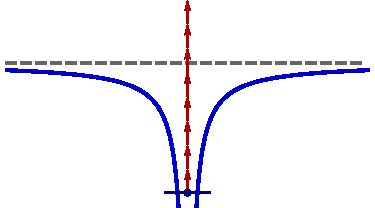
\includegraphics[scale=1]{1-Introduction/Figures/figure1Aa.pdf}
  }
  \hspace{3mm}
  \subfigure[Tunnelling picture]{
    \label{f1-tunnelling-picture}
    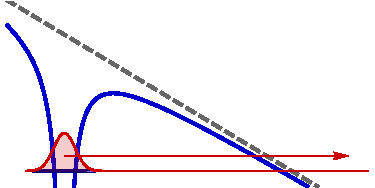
\includegraphics[scale=1]{1-Introduction/Figures/figure1Ab.pdf}
  }
  \caption[Basic pictures of strong field ionization]{
  Basic pictures of strong field ionization: \protect\subref{f1-multiphoton-picture} the multiphoton picture, in which an electron absorbs multiple energy quanta from the external field, and \protect\subref{f1-tunnelling-picture} the tunnelling picture, in which the external potential $V_L = -Fx\cos(\omega t)$ tilts the potential landscape enough to form a barrier the bound wavefunction can tunnel through.
  }
\label{f1-basic-pictures}
\end{figure}

As shown by Keldysh, these two pictures are actually two different sides of the same coin, and they are only truly valid  as limiting behaviours. More concretely, if we consider the ionization of a system with ionization potential $I_p=\frac12 \kappa^2$ by a monochromatic field of the form $F\cos(\omega t)$, with angular frequency $\omega$ and electric field amplitude $F$, then much of the behaviour is governed by the Keldysh adiabaticity parameter,
\begin{equation}
\gamma = \frac{\kappa \omega}{F} = \sqrt{\frac{I_p}{2U_p}},
\label{e1-keldysh-parameter}
\end{equation}
often called simply the Keldysh parameter. Here we assume that the field is `slow', or that the target is `hard', in the sense that $\omega\ll I_p$, and it takes multiple photons to ionize the system. 

However, there is a separate timescale to consider -- the time it takes for the electron to tunnel through the barrier at the peak of the field, which can be estimated using quasi-static arguments~\cite{landau_QM} as $\tau_\mathrm{tunn}\sim\kappa/F$. Thus, if the field changes slowly enough to permit appreciable tunnelling, in the regime of low $\gamma\propto\omega$, the behaviour is mostly in the tunnelling picture. Conversely, if the field is too fast or too weak for this, and $\gamma$ stays high, then the ionization mostly displays multi-photon picture features that can mostly be explained through a perturbation-theory viewpoint.

Alternatively, the Keldysh parameter can also be seen as the relationship between the energy scales of the ground state energy, $-I_p$, and the ponderomotive potential \mbox{$U_p=F^2/4\omega^2$}, which is the average oscillatory energy of an electron moving in the field. Thus, at low $\gamma$, the oscillatory motion has much more energy than that required to ionize the electron in the first place, and vice versa.




\subsection{A quick note on units}
Throughout this thesis we will use the atomic system of units, unless otherwise noted. This system of units is fixed by taking the essential dynamical quantities of atomic physics as unity,
\begin{equation}
\hbar = m_e = e^2 = \frac{1}{4\pi\eps_0} = 1,
\end{equation}
and it is reviewed more fully in Appendix~\ref{chap:atomic-units}. Also note that, to avoid confusion between energies and electric fields, we denote the latter with the letter $F$ throughout.%
\footnote{%
Since we're discussing style, this is a good place to apologize for the use of the plural first person throughout this thesis. This is relatively awkward, but the singular first person is even worse, and passive constructions are the bane of readability. The author invites the reader to include his or herself in this scientific `we', or (if that is uncomfortable) to include the immortal F.D.C. Willard in that plural first~person.
}



\subsection{Essential approximations}

To make our treatment more concrete, we now need to start approximating, since the full Schrödinger equation requires the brunt of a numeric integrator to handle in full. There are several key approximations that we need to make, with varying degrees of generality (and some of which we will discard later on).

\begin{itemize}
\item We will work throughout using non-relativistic quantum mechanics, an approximation that states that the laser field may well move the electrons fairly violently, but it will keep them at a reasonable fraction of the speed of light; this sets an upper limit of field strength at about $\SI{e16}{W/cm^2}$ (at which field strength most species get multiply ionized), and we will stay below that regime. 

In chapter~\ref{chap:nondipole-HHG} we will come somewhat close to relativistic velocities but, for the observables of interest there, a full relativistic treatment is not necessary.

\item In addition, we will also work, with the exception of chapter~\ref{chap:nondipole-HHG}, within the dipole approximation. In general, if we have a non-relativistic electron subject to an atomic potential $V(\vbr)$ and interacting with a laser field of vector potential $\vba(\vbr,t)$ of the external field (which we always take in the radiation gauge, and which relates to the electric field via $\vbf(\vbr,t)=-\frac{\partial \vba}{\partial t}(\vbr,t)$), then the minimal coupling hamiltonian reads
\begin{equation}
\hat H = \frac{1}{2} \left(\vbp +\vba(\vbr,t)\right)^2 + V(\vbr).
\end{equation}
In general, the spatial variation of the vector potential $\vba(\vbr,t)$ will be on the order of the wavelength $\lambda$ of the laser; the shortest such wavelength that we will consider will be $\SI{400}{nm}$, on the order of $\SI{1000}{\au}$ In a strong field context, the electron can make some very long excursions, but these will typically be smaller than the wavelength (and, moreover, will tend to be orthogonal to the propagation direction). 

%%%Note hackish \au-period above

This means, then, that we can safely replace the vector potential with its value at the nucleus of our atom of interest (or, with molecules, at the nuclear centre of charge), getting a hamiltonian of the form 
\begin{equation}
\hat H = \frac{1}{2} \left(\vbp +\vba(\vb 0,t)\right)^2 + V(\vbr).
\label{e1-velocity-gauge-hamiltonian}
\end{equation}
We will term hamiltonians of this form as being in the \textit{velocity gauge}, since the interaction hamiltonian in $\hat H = \frac{1}{2} \vbp^2 + V(\vbr) + \vba(\vb0,t)\cdot\vbp +\vba(\vb0,t)^2$ couples directly to the velocity operator $\vbp$.

Working in the dipole approximation allows us to change to a more convenient gauge, which we will term the \textit{length gauge}, via the unitary transformation $\hat U=e^{-i\vba(\vb0,t)\cdot\hat\vbr} e^{-\frac i2\int \vba(\vb0,t)^2\d t}$, which gives the length-gauge hamiltonian as 
\begin{equation}
\hat H = \frac{1}{2} \vbp^2 + V(\vbr) - \vbr\cdot\vbf(\vb0,t).
\label{e1-length-gauge-hamiltonian}
\end{equation}

As a separate effect, within the dipole approximation the vector potential has no spatial dependence, which means that its magnetic field $\vb B(\vbr,t)=\nabla \times \vba(\vbr,t)$ necessarily vanishes. In chapter~\ref{chap:nondipole-HHG} this will push us to discard the dipole approximation but unless one works at extremely high intensities or at very long wavelengths (which, as we shall see, can also cause a breakdown of the dipole approximation), the magnetic field is negligible.  (Finally, for notational convenience, and unless it is required for clarity, we will henceforth drop the spatial indicator $\vb0$.)





\item While this is seldom made explicit in more recent strong-field physics, most of what follows requires that the laser pulse be short enough for the laser pulse to end before the photoelectron can leave the focus, which in practice needs pulses shorter than some hundreds of femtoseconds. If this fails, then one needs to consider the effect on the photoelectron's momentum of the edge of the focus, which will drastically change the structures of interest; moreover, a long pulse can quite easily saturate the ionization. Pulses of this length are, of course, perfectly accessible to modern light sources and indeed they are required to attain the intensities at play.


\item Moreover, we will work in the clamped-nucleus approximation, both for the handling of atoms and with molecules, leaving the nuclei at their equilibrium separation. 
\end{itemize}


In addition to these approximations, most of strong-field physics works rather well under what is known as the Single-Active Electron (SAE) approximation, which is implicit in both the hamiltonians in \eqref{e1-velocity-gauge-hamiltonian} and \eqref{e1-length-gauge-hamiltonian} above: in general, much of strong-field phenomena can be understood rather well by assuming that each electron acts independently, neglecting the effects of electron correlation and exchange, and that the rest of the electrons in the system act only to provide the effective potential $V(\vbr)$.

The single-active electron approximation is remarkably effective, mostly due to the fact that a strong laser field will typically take the active electron far away from the rest of the system rather quickly, and it will afterwards be dynamically very different from the remaining electrons, even if it comes back to do diffractive imaging. In fact, it works well even in non-sequential double ionization via recollision mechanisms, where the pre-recollision dynamics can essentially be done with a single active electron.

On the other hand, there are multiple reasons to go beyond the single-active electron paradigm, which we will recount in more depth in chapter~\ref{chap:multi-channel}, especially driven by the fact that the ion can be left in an excited state after the pulse is over. While this can happen through single-electron mechanisms, essentially by removing an electron from an orbital below the highest-occupied one, there is increasing evidence that electron correlation can play a role in this process. 

To accommodate for this we will build a multi-electron theory in chapter~\ref{chap:R-matrix} and examine it in more detail in chapters~\ref{chap:multi-channel} and~\ref{chap:complex-space-potentials}, before reverting to single-electron phenomena for the rest of the thesis. For the moment, we will show a sketch of the Strong-Field Approximation, as developed by Keldysh, within the single-active electron approximation.



\subsection{The Strong-Field Approximation}


This leaves us, then, with the final core approximation of analytical strong-field physics, the stipulation that after the ionization step the photoelectron is at the mercy of the radiation field, if it is strong enough, and that the electric field of the ion plays, at most, a perturbative role. This can be done in a number of different ways, giving slightly different approaches, many of which are grouped under the name of the Strong-Field Approximation, despite their (sometimes substantial) differences. We will not delve into the various formulations of this approximation, which has been reviewed elsewhere~\cite{popruzhenko_Keldysh_theory, galstyan_sfa-reformulation_2016}; instead, we will give a sketch of Keldysh's original approach and then discuss the generalities of the overall method.


We begin, then, with the Schrödinger equation in the presence of the laser field, in the~form
\begin{equation}
i\frac{\d}{\d t}\ket{\psi(t)}
=\hat H \ket{\psi(t)}
=\left[ \frac12 \vbp^2 + V(\vbr) + \vbr\cdot \vbf(t) \right]\ket{\psi(t)},
\label{e1-sfa-tdse}
\end{equation}
where we are assuming a single active electron and working in the length gauge. As an initial condition, we take the electron to sit in the ground state of the system, $e^{-iE_gt}\ket{\psi_g}$, before the pulse starts. The core of the Strong-Field Approximation, as a method, is to assume, first, that this is the only bound state of the system that will contribute to the dynamics (though, again, that can be relaxed~\cite{perez-hernandez_sfa-plus_2009}). We postulate, then, an Ansatz of the form
\begin{equation}
\ket{\psi(t)} = e^{-iE_g t}\ket{\psi_g} + \ket{\psi_\mathrm{out}(t)},
\label{e1-keldysh-ansatz}
\end{equation}
where $\ket{\psi_\mathrm{out}(t)}$ is the outgoing continuum electron.

(Here it is important to remark that, although physics should in principle be fully gauge-indepen\-dent, as will be much of our handling of $\ket{\psi_\mathrm{out}(t)}$, the Ansatz in \eqref{e1-keldysh-ansatz} is not gauge independent, since we are performing an approximation by trimming down the complete set of bound states to just a single component, so this is actually a different approximation if performed in the velocity gauge~\cite{galstyan_sfa-reformulation_2016}, which can correspondingly lead to different results.)

In addition to the bound-state Ansatz in \eqref{e1-keldysh-ansatz}, the Strong-Field Approximation also completely ignores the role of the atomic potential $V(\vbr)$ once the electron is in the continuum, so the outgoing wave-packet obeys the laser-only Schrödinger equation,
\begin{equation}
i\frac{\d}{\d t}\ket{\psi_\mathrm{out}(t)}
=\left[ \frac12 \vbp^2 + \vbr\cdot \vbf(t) \right]\ket{\psi_\mathrm{out}(t)}.
\end{equation}
This equation can, fortunately, be solved exactly,%
%
\footnote{
Incidentally showing that exact solutions in quantum mechanics are not confined to the harmonic oscillator as the go-to system. Instead, it is also perfectly possible to solve for a particle in a uniform force field, even with an arbitrary time dependence.
}
%
and moreover it admits solutions which are plane waves throughout, known as Volkov states. These are given by
\begin{equation}
\braket{\vbr}{\Psi^\mathrm{(V)}_{\vbp}(t)}
=
\frac{1}{(2\pi)^{3/2}}
e^{i(\vbp+\vba(t))\cdot\vbr}
e^{-\frac i2 \int_{T}^t \left(\vbp+\vba(\tau)\right)^2 \d\tau}
,
\label{e1-volkov-wavefunctions}
\end{equation}
and they have a kinetic momentum $\vbv(t)=\vbp+\vba(t)$ which oscillates with the laser field, accruing phase via the kinetic energy $\frac12 \vbv(t)^2$. 

The Volkov states are excellent building blocks, and we will later modify them to account for the Coulomb field of the ion, to give the eikonal-Volkov states of chapter~\ref{chap:R-matrix}, and to include the magnetic field of the driver, giving us non-relativistic non-dipole Volkov states in chapter~\ref{chap:nondipole-HHG}. For the moment, though, we keep them as they are.


This means that we can re-phrase our Ansatz in the form
\begin{equation}
\ket{\psi(t)} 
= 
e^{-iE_g t}\ket{\psi_g} 
+ \int \d\vbp \,a(\vbp,t) \volkov{\vbp}{t}, 
\label{e1-keldysh-full-ansatz}
\end{equation}
where $a(\vbp,t)$ is the time-dependent amplitude of each Volkov state, which we need to solve for. This Ansatz comes with the assumption that $\braket{\psi_g}{\Psi^\mathrm{(V)}_{\vbp}(t)} \approx 0$ for all canonical momenta $\vbp$, which is clearly wrong, but it does a good job at specifying the separation of the active Hilbert space into a bound-state component and a field-driven continuum. 

We have, then, a full Ansatz for the wavefunction, \eqref{e1-keldysh-full-ansatz}, which now allows us to put it into the Schrödinger equation to get the dynamics. Since we have included most of the dynamics already into our bound and continuum components, the Schrödinger equation simplifies a good deal, to give
\begin{align}
\left(
i\frac{\d}{\d t}
-\hat H
\right)\ket{\psi(t)}
& =
-\vbr\cdot\vbf(t) e^{-iE_g t}\ket{\psi_g}
+ \int \d\vbp \,
\left( 
i\frac{\partial a}{\partial t}(\vbp,t) 
-V(\vbr)a(\vbp,t)
\right)
\volkov{\vbp}{t}
,
\end{align} 
or, projecting on the Volkov state $\volkov{\vbp}{t}$,
\begin{align}
i\frac{\partial a}{\partial t}(\vbp,t)
& =
e^{-iE_g t}\matrixel{\Psi_{\vbp}^\mathrm{(V)}(t)}{\vbr\cdot\vbf(t)}{\psi_g}
%\nonumber \\ & \qquad
+\int \d\vbp' \,
a(\vbp',t)
\matrixel{\Psi_{\vbp}^\mathrm{(V)}(t)}{V(\vbr)}{\Psi_{\vbp'}^\mathrm{(V)}(t)}
.
\end{align}
Here we perform our final approximation by neglecting the second term, which represents continuum-continuum transitions induced by the atomic potential, i.e. scattering on the atomic core, which is again outside of the SFA (though it can be put back in to account for rescattered electrons in ATI~\cite{milosevic_ISFA-standard_2007}).

The Schrödinger equation thus reduces to a simple ordinary differential equation, and its solution can be stated simply in terms of a time integral in the form
\begin{align}
a(\vbp)
& =
-i
\int_{-\infty}^{\infty} \!
e^{iI_p t+\frac i2 \int_{\tn}^{t} \left(\vbp+\vba(\tau)\right)^2 \d\tau}\matrixel{\vbp+\vba(t)}{\vbr\cdot\vbf(t)}{\psi_g}
\, \mathrm dt
.
\label{e1-keldysh-integral-result}
\end{align}
(Here we have set $I_p=-E_g>0$ for convenience, extracted the explicit phase and plane wave $\ket{\vbp+\vba(t)}$ from the Volkov state, and asked for the amplitude at $t\to\infty$ after the pulse is over.)  This is, essentially, the main final answer from the Keldysh-style SFA, though we will analyse it further below. 




\subsection{Imaginary time and trajectory language}
The result in \eqref{e1-keldysh-integral-result} closes an impressive gap, by taking the full TDSE and reducing it to a single integral per final momentum $\vbp$, so it can be queried directly and easily. However, it can still be simplified considerably by suitably modifying the integration path into the complex plane. 

We will analyse  this in more detail in chapter~\ref{chap:R-matrix}, but it is easy to see that the integral is highly oscillatory, since it includes a factor of $e^{iI_pt}$ being integrated on the scale of several laser cycles, and we are working in the regime where $\omega \ll I_p$. (There is an additional average factor of $e^{iU_pt}$ coming from the kinetic term of the phase, which is even larger for $\gamma<0$, but this only increases the severity of the problem.) This makes the numerical integration of \eqref{e1-keldysh-integral-result} challenging, since one the final value comes through heavy cancellations, so one needs to compute each lobe to very high accuracy to get only moderate precision on the final result, or use sophisticated integration algorithms that attempt to account for this.

The most efficient approach, however, is to recur to the tools of complex analysis in the form of the \textit{saddle-point approximation}. We will explain this in depth in chapter~\ref{chap:R-matrix} (and there are good reviews in Refs.~\citealp{popruzhenko_Keldysh_theory} and \citealp{Popov_imaginary_time}), but the essence is that one can modify the integration path of \eqref{e1-keldysh-integral-result} away from the real axis in a way that turns the oscillatory exponential 
\begin{equation}
e^{-iS(\vbp,t)} = \exp({iI_p t+\frac i2 \int_{T}^{t} \left(\vbp+\vba(\tau)\right)^2 \d\tau})
\label{e1-sfa-action}
\end{equation}
into a series of gaussian bumps with a flat phase, which essentially reduce to the contributions from a discrete series of points at the top of those gaussians. These are the saddle points $\ts$ of the exponent $S(\vbp,t)$, which satisfy the core saddle-point equation
\begin{equation}
\frac{\partial S}{\partial t}(\vbp,\ts) = 0,
\label{e1-initial-saddle-point-equation}
\end{equation}
which make the phase stationary. In addition, a quick look at $S(\vbp,t)$ shows that it is the kinetic action of an electron in the laser field, so the condition \eqref{e1-initial-saddle-point-equation} is a form of the principle of stationary action (and, indeed, the connection to Feynman's path integral formalism can be made explicit and rigorous~\cite{salieres_quantum_orbits}).

The result, then, is an approximation to the ionization yield $a(\vbp)$ in the form of the sum of the integrand over a discrete collection of saddle points $\ts$, chosen by the ability to deform the integration path to reach them, in the form
\begin{equation}
a(\vbp)
=
\sum_{\ts}
\sqrt{\frac{2\pi}{i\partial^2 S/\partial t^2(\vbp,\ts)}}
e^{-iS(\vbp,\ts)} 
\matrixel{\vbp+\vba(\ts)}{\vbr\cdot\vbf(\ts)}{\psi_g}
.
\label{e1-saddle-point-result}
\end{equation}
More appealingly, this form also gives us a compelling physical picture which we can just read off: the electron, originally in the ground state $\ket{\psi_g}$, performs a transition at a time $\ts$ through the laser coupling $\vbr\cdot\vbf(\ts)$ to a continuum state with initial kinetic momentum $\vbp+\vba(\ts)$ (which, moreover, can be shown to have vanishing velocity along the laser polarization), and it then propagates classically accruing action exactly as a free electron in the laser field, via
\begin{equation}
S(\vbp,t) =-I_p t-\frac 12 \int_{\tn}^{t} \left(\vbp+\vba(\tau)\right)^2 \d\tau
,
\label{e1-sfa-action-real}
\end{equation}
with a factor of $\sqrt{\frac{2\pi}{i\partial^2 S/\partial t^2(\vbp,\ts)}}$ as a remainder of the time integration. There will be, in principle several  of these trajectories, and we simply add their probability amplitudes as~usual. Each such factor, in turn, can be directly interpreted as coming from a single trajectory ionized at time $\ts$ and evolving with velocity $\vbv(t)=\vbp+\vba(t)$.


There is a problem, of course, and it is that the saddle-point times $\ts$ generally do not lie on the real axis, and that therefore we do need to modify the integration path in \eqref{e1-keldysh-integral-result} to reach them. This is not very problematic when we are talking about the amplitudes -- they are just some mathematical function in a convenient and compact form~-- but it raises some serious conceptual issues when we attempt to understand each individual term in the sum as corresponding to a classical trajectory. What does it mean for an electron to be ionized at a complex time? What is the physical meaning of that ionization time, and can it be measured experimentally? What does the trajectory look like, and what does it mean physically? These questions have plagued the field since Keldysh first raised the issue~\cite{keldysh_ionization_1965}, and they do not yet have satisfactory answers.


The usual way of understanding the complex ionization times $\ts$ is to get away from them as fast as possible: that is, if we need to visualize the passage of time for the electron from its ionization at $\ts = \tn +i\tauT$, we normally first take it straight down to the real part $\tn=\Re(\ts)$, and we can then take it along the real axis more normally, as shown~in~\reffig{f1-initial-contour}.

\begin{figure}[ht]
  \centering
  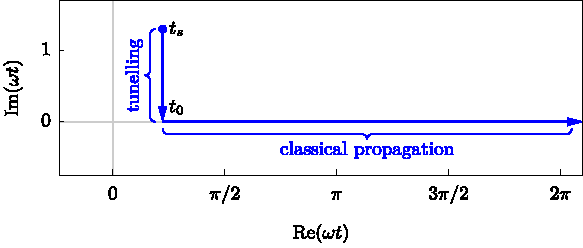
\includegraphics[scale=1]{1-Introduction/Figures/figure1B.pdf}
  \caption[Standard contour from the complex ionization time $\ts$ to its real part $\tn$ and then along the real axis]{
  Standard contour for understanding trajectories in complex time going from the complex ionization time $\ts$ to its real part $\tn$ and then along the real axis until the final detection at a large, real time.
  }
\label{f1-initial-contour}
\end{figure}

This has the advantage of clearly delineating the roles of each part of the contour, and it matches rather well our understanding of how tunnel ionization should work: the downwards part of the path takes place in complex time, so $S(\vbp,t)$ will be complex and $e^{-iS(\vbp,t)}$ will be a strong modulation on the amplitude; similarly, on the classical propagation part the velocity and action are now real, and everything behaves much as Feynman originally described it, with a (restricted) set of classical trajectories that are eventually added with probability amplitude $e^{-iS(\vbp,t)}$. Even better, the `tunnel exit' in this formalism, $\int_{\ts}^{\tn}\left[\vbp+\vba(t)\right]\d t$, can be shown to reduce to the usual $I_p/F$ in the quasistatic $\gamma \ll 1$~limit.


In addition to being very appealing, this classical understanding very often works, and can be very effective. One very pervasive way to implement this is to use the above formalism purely to obtain the tunnelling rate down to the real axis, and then to completely forget about quantum mechanics: to consider \eqref{e1-saddle-point-result} as describing the emergence at time $\tn$ of an electron with zero longitudinal velocity with probability
\begin{equation}
\left|
\sqrt{\frac{2\pi}{i\partial^2 S/\partial t^2(\vbp,\ts)}}
\matrixel{\vbp+\vba(\ts)}{\vbr\cdot\vbf(\ts)}{\psi_g}
\right|^2
\times
e^{2\Im\left(S(\vbp,\ts)\right)} 
,
\end{equation}
and then to propagate these trajectories classically, either under the laser driving only or also including the effect of the ionic potential.%
\footnote{%
Generally, this is changed to the ADK rates~\cite{ammosov-delone-krainov-1986}, to include the effect of the Coulomb potential during the tunnelling step, but this does not change the fundamentals.
}
This method, known generally as the classical-trajectory Monte Carlo (CTMC) approach, can be very effective, and we will meet it again in chapter~\ref{chap:LES-NZES}.

However, this method, and others like it, is essentially only a model: it is grounded in a calculation from the TDSE, but eventually it departs from it and works by analogy, introducing the constructs that look appropriate (like, for example, the effect of the ionic potential on the trajectory) in a form that fits into its environment, and hoping for the result to match experimental measurements. As a model, the CTMC approach has a number of successes (as do its several analogues), but it is very thinly grounded on the Schrödinger equation. 

This is, in a way, one of the key problems that this thesis tackles: can one derive a trajectory-based model, which allows one among other things to describe the interactions with the ion's potential, directly from the Schrödinger equation, and without proceeding by analogy or similar leaps? As we will see, this is indeed possible, but it comes at the cost of having a complex-valued trajectory once the time reaches the real axis. Moreover, this imaginary component of the position is retained all the way to the detector, it has a very strong effect on the interaction with the ion, and it ultimately makes the standard contour shown in \reffig{f1-initial-contour} inadmissible and essentially meaningless. 

In essence this is because the imaginary component of the position combines with the Coulomb potential of the ion, $-1/\sqrt{\vbr^2}$, to produce branch cuts in the complex time plane that severely restrict the paths the trajectory can take, and we will show how to navigate these branch cuts to obtain suitable paths in the complex time plane. This method will then allow us to explain intricate structures that appear in the low energy region of ATI spectra. More recently, the inclusion of this imaginary component of the position has also been shown to be crucial in explaining higher-energy phenomena~\cite{keil_branch-cuts_2016}, in the intersection of direct and rescattered ATI electrons, with our method of branch cut navigation successfully allowing the evaluation of correct trajectories, at the expense of the foot $\tn$ of the standard contour as a central concept of the theory.








\subsection{Including the Coulomb field of the ion}
Coming back to the Keldysh result \eqref{e1-saddle-point-result}, it is also important to remark that, for all its conceptual and quantitative successes, the Keldysh theory does have some serious limitations. One of them is the limitation to relatively weak fields limited by $F\ll \SI{1}{\au}$, so the theory only works in the tunnelling regime, where the barrier still exists, and it fails for over-the-barrier ionization where the potential in \reffig{f1-tunnelling-picture} dips below the energy of the ground state, liberating the wavefunction and ensuring very swift and complete ionization. 

(In general, however, this is not too hindering a limitation, since if a pulse goes above that intensity then the leading edge, which still falls within the tunnelling limits, is very likely to saturate the ionization, presenting the higher fields in the middle of the pulse with a harder target with a higher ionization potential that is often still inside the tunnelling regime, now modified to $F\ll (2I_p)^{3/2}$.)


More seriously, on the other hand, the Keldysh theory is limited to only short-range potentials, and it produces very poor quantitative results when applied to charged systems with an asymptotic Coulomb potential, often out by several orders of magnitude (even if the shape of the spectrum is relatively accurate). As such, one of the key goals of the theory of strong-field physics is to have an analytical theory -- ideally sharing as much of the SFA's conceptual and computational simplicity -- that includes this Coulomb potential.


Several approaches have extended the Keldysh method to include the Coulomb potential, most notably by A.~M. Perelomov, V.~S. Popov and M.~V. Terent'ev~\cite{perelomov_ionization_1966, perelomov_ionization-II_1967, perelomov_ionization-III_1967} for a nonzero charge, known as the PPT model, and later simplified by M. Ammosov, N. Delone and V. Krainov~\cite{ammosov-delone-krainov-1986}, dealing with arbitrary initial states, giving the so-called ADK rates that extend well to the case of molecules~\cite{tong_mo-adk_2002}. However, extending these methods to observables beyond the ionization rate has proved challenging, and though there are several interesting methods available there is as yet no completely satisfactory theory for~this.




\subsubsection{PPT methods}
The core method for including the Coulomb field into the SFA ionization rates was provided by Perelomov et al. in \citer{perelomov_ionization-II_1967}, and it can be simplified a good deal by phrasing it in trajectory language~\citer{perelomov_ionization-III_1967}, which can then be modified to include the Coulomb field in a relatively ad-hoc way. Using integration by parts, one can rephrase the action \eqref{e1-sfa-action} as
\begin{align}
S(\vbp,t) 
&=
-I_p t+\frac 12 \int_{T}^{t} \left[\vbv(\tau)^2 + \vbr(\tau)\cdot \dot{\vbv}(\tau) \right] \d\tau
\nonumber \\ &=
-I_p t + \int_{T}^{t} \left[\frac 12 \vbv(\tau)^2 - \vbr(\tau)\cdot \vbf(\tau) \right] \d\tau
,
\label{e1-sfa-action-lagrangian}
\end{align}
where $\vbr(t)=\int_{t_\mathrm{ref}}^{t}\left[ \vbp+\vba(\tau)\right] \d\tau$ and $\dot\vbv(t) = \frac{\d\vba}{\d t} =-\vbf(t)$, and this is explicitly in the form of a lagrangian function $L=\frac 12 \vbv(\tau)^2 - \vbr(\tau)\cdot \vbf(\tau)$ with an explicit potential. To include the Coulomb potential here, and working in analogy to our original hamiltonian from \eqref{e1-sfa-tdse}, we can simply expand this to
\begin{equation}
L=\frac 12 \vbv(\tau)^2 - \bigg[ \vbr(\tau)\cdot \vbf(\tau) +V(\vbr(\tau)) \bigg].
\end{equation}
This requires some amount of care, since integrating $\int V(\vbr(\tau))\d\tau$ can produce infinities coming from the $1/r$ singularity at the origin, but in general these can be appropriately regularized. However, it is relatively challenging to extend this to a full photoelectron momentum spectrum, and the theory misses some non-adiabatic tunnelling effects, which come from the temporal variation of the barrier, for Coulomb potentials. As such, in general the use of PPT methods in the recent literature is mostly seen in calculations of total rates or, through the extension to ADK~\cite{ammosov-delone-krainov-1986} and molecular ADK~\cite{tong_mo-adk_2002} to arbitrary atomic and molecular states, respectively, for the calculation of instantaneous tunnelling rates, down to the tunnelling `foot' of the integration, for CTMC calculations. 



\subsubsection{Coulomb-Corrected Strong-Field Approximation}
The ideas of the PPT method reach their full fruition in what's generally known as Coulomb-corrected SFA methods (CCSFA), first introduced by S.~V. Popruzhenko and co-workers in Refs.~\citealp{CCSFA_initial_short, CCSFA_initial_full, popruzhenko_ccsfa-arbitrary-frequency_2008, popruzhenko_multiphoton_2009}. In essence, these methods take the SFA expression for the ionization amplitude, 
\begin{equation}
a(\vbp)
=
\sum_{\ts}
\sqrt{\frac{2\pi}{i\partial^2 S/\partial t^2(\vbp,\ts)}}
e^{-iS(\vbp,\ts)} 
\matrixel{\vbp+\vba(\ts)}{\vbr\cdot\vbf(\ts)}{\psi_g}
,
\backtag{e1-saddle-point-result}
\end{equation}
and retain its form, modifying only the action, both in terms of its explicit form as well as the trajectory that it is evaluated on. 

In general, this usually means expanding to first order about the laser-driven system, with trajectory $\vbr_0(t)=\int_{t_\mathrm{ref}}^{t}\left[ \vbp+\vba(\tau)\right] \d\tau$  and the action \eqref{e1-sfa-action-lagrangian}, to include the Coulomb potential in the latter via
\begin{align}
S_{\textsc{ccsfa}}(\vbp,t) 
&=
-I_p t + \int_{T}^{t} \left[\frac 12 \dot{\vbr}(\tau)^2 - \vbr(\tau)\cdot \vbf(\tau) \right] \d\tau
-\int_{T}^t V(\vbr(\tau))\d\tau
,
\label{e1-ccsfa-action-lagrangian-coulomb}
\end{align}
and to expand the trajectory to $\vbr(t) = \vbr_0(t) + \vbr_1(t)$, where $\vbr_0(t)$ is the laser-driven trajectory and, in lieu of the full equation of motion
\begin{equation}
\ddot \vbr(t) = -\vbf(t) -\frac{Z\vbr(t)}{\|\vbr(t)\|^3},
\label{e1-ccsfa-equation-of-motion-full}
\end{equation}
it is often sufficient to take only a first-order correction,
\begin{equation}
\ddot \vbr_1(t) = -\frac{Z\vbr_0(t)}{\|\vbr_0(t)\|^3}.  \phantom{-\vbf(t)}
\label{e1-ccsfa-equation-of-motion-first-order}
\end{equation}
These methods can be put together in different combinations (so, for example, the correction to the action can be left only as $-\int_{T}^t V(\vbr_0(\tau))\d\tau$, or the corrections to the trajectory may be discarded), depending on the conditions of the problem.

In addition to this, the CCSFA methods typically require the canonical momentum $\vbp'$~at ionization to be different to the final momentum $\vbp$ at the end of the pulse, because the equations of motion (\ref{e1-ccsfa-equation-of-motion-full}, \ref{e1-ccsfa-equation-of-motion-first-order}) do not conserve the canonical momentum as the laser-only evolution does. This poses a problem, because when we evaluate a photoelectron momentum spectrum we usually fix a final momentum $\vbp$, and we want to calculate its ionization amplitude; this is an inverse problem (given a final momentum, find the initial conditions that lead to it), but the CCSFA postulates are posed as a forward one (given initial conditions they produce the final momentum). This can be solved via a `shotgun' approach to the momentum, by seeding a large number of initial conditions and seeing what their final momentum is. The procedure requires some care (such as when calculating the interference between trajectories whose final momenta almost, but do not quite, match), but it can be done with a framework that is essentially as efficient and flexible as the original SFA.


A somewhat more problematic issue, however, is the setting of the initial conditions for the trajectories. The SFA trajectory language tells us a fair amount about the trajectories, most notably through their velocity $\vbv(t)=\vbp+\vba(t)$, but it is mute about where the trajectory starts. This is required information to compute the trajectory via the equations of motion~(\ref{e1-ccsfa-equation-of-motion-full}, \ref{e1-ccsfa-equation-of-motion-first-order}), and it is similarly necessary to compute the Coulomb action in~\eqref{e1-ccsfa-action-lagrangian-coulomb} even if only the zeroth-order trajectory is used, via $-\int_{T}^t V(\vbr_0(\tau))\d\tau$. 

Thus, the CCSFA method requires an initial condition to be put in externally, which can be done but it means that the formalism is firmly on the class of a model that proceeds by analogy. It is certainly very successful, and it correctly explains, among other things, the Coulomb-enhanced ionization rate~\cite{popruzhenko_ccsfa-arbitrary-frequency_2008} and the breaking of the SFA's excessive symmetry in an elliptically polarized field~\cite{CCSFA_initial_short, CCSFA_initial_full}. However, it does not derive directly from a TDSE, which makes it desirable to find an analogous theory that does proceed from first principles and arrives at a similar trajectory-based intuitive understanding of the ionization process.






\subsubsection{Coulomb-Volkov Approximation}
On a separate approach to the inclusion of the Coulomb potential is what is known as the Coulomb-Volkov Approximation (CVA)~\cite{jain_coulomb-volkov_1978,cavaliere_coulomb-volkov_1980}, which essentially consists of replacing the Volkov states in the SFA results -- both the integral version~\eqref{e1-keldysh-integral-result}, and from there to the saddle-point result~\eqref{e1-saddle-point-result} -- with Coulomb-modified scattering waves that incorporate spatial aspects of the Coulomb waves $\ket{\Psi_{\vbp}^{(-)}}$ in addition to Volkov-state behaviour; more specifically, of the form
\begin{align}
\braket{\vbr}{\Psi_{\vbp}^\mathrm{(CV)}(t)}
& =
e^{i\vba(t)\cdot\vbr - \frac i2\int_{-\infty}^t \vbv(\tau)^2\d\tau}
\braket{\vbr}{\Psi_{\vbp}^{(-)}(t)}
 \\ & = 
\frac{e^{\pi/2p}}{(2\pi)^{3/2}}
\Gamma\mathopen{}\left(1+\frac{i}{p}\right)\mathclose{}
{}_1F_1\left( -\frac{i}{p},1,-i(pr+\vbp\cdot\vbr)\right)
e^{i\vbp\cdot\vbr}
e^{i\vba(t)\cdot\vbr}
e^{-\frac i2\int_{-\infty}^t \vbv(\tau)^2\d\tau}
\nonumber
,
\end{align}
where ${}_1F_1$ is a confluent hypergeometric function~\citenistchap{13}. The Coulomb-Volkov approximation is, again, a relatively successful model, explaining things like Coulomb focusing and angular distributions at low energy in the multiphoton regime~\cite{arbo_coulomb-volkov_2008}. However, the CVA is problematic, partly because it is difficult to extend to more complicated potentials, and partly because the relatively ad hoc introduction of $\ket{\Psi_{\vbp}^\mathrm{(CV)}(t)}$ makes it difficult to gauge the approximation's conditions of validity~\cite{ popruzhenko_Keldysh_theory}.







\subsubsection[Analytical R-Matrix theory]{Analytical $R$-Matrix theory}
The work in this thesis is based on a separate approach to the inclusion of Coulomb effects into SFA-like theories, known as the Analytical $R$-Matrix (ARM) theory of ionization~\cite{torlina_thesis, kaushal_thesis, ARM_initial, ARM_initial_multielectron}; we will build it in detail in chapter~\ref{chap:R-matrix}, but we present here a sketch of the fundamentals. 

The basic idea is to track the origin of the SFA trajectory language, which essentially comes from the $e^{-iS}$ form of the Volkov continuum wavefunctions~\eqref{e1-volkov-wavefunctions}. As such, if one wants to expand this trajectory language to include the effects of the Coulomb potential on the continuum electron, the best place to do it is directly at the level of its original wavefunction.

Fortunately, this can indeed be done, in a formalism known as the eikonal-Volkov approximation (EVA)~\cite{eikonalVolkov_prelim, eikonalVolkov_initial}. In essence, this entails adding a phase correction to the Volkov states~\eqref{e1-volkov-wavefunctions}, of the form 
\begin{align}
\braket{\vb{r}}{\Psi_{\vbp}^{\mathrm{(EVA)}}(t)}
& = 
%P_\textsc{EVA}(\vbp,\vbr,t)
e^{iS_\textsc{EVA}(\vbp,\vbr,t)/\hbar}
\braket{\vb{r}}{\Psi_{\vbp}^{\mathrm{(V)}}(t)}
,
\label{e1-eikonal-volkov-essential-ansatz}
\end{align}
and then solving the full Schrödinger equation~\eqref{e1-sfa-tdse}, with the Coulomb field taken as a perturbation, giving a solution as a series in $\hbar$ (which is of course subsequently reverted to~$\hbar=1$). The result, not surprisingly, is very similar to the CCSFA action, as an integral of the ionic potential $V(\vbr)$ over a trajectory,
\begin{equation}
S_\textsc{EVA}(\vbp,\vbr,t) = -\int_T^t V(\rl(\tau;\vbr,\vbp,t))\d\tau
,
\label{e1-eva-action}
\end{equation}
where now the trajectory starts at the probing point $\vbr$ at time $t$, and is driven exclusively by the laser until it reaches an asymptotic canonical momentum $\vbp$:
\begin{equation}
\rl(\tau;\vb{r},\vbp,t)
=
\vb{r}+\int_t^\tau \left[\vbp+\vba(\tau')\right]\d\tau'
.
\label{e1-eva-trajectory}
\end{equation}


This gives us, then, a trajectory-based Coulomb-corrected continuum wavefunction, though in the language of CCSFA it is only corrected to first order in the action, and it is taken to zeroth order on the trajectory. As we will discuss in chapter~\ref{chap:quantum-orbits}, it would be desirable to have trajectory-based Coulomb-corrected continuum wavefunctions with higher order corrections in the trajectory, but this is a very challenging problem which does not appear particularly accessible with currently available tools. On the other hand, the action \eqref{e1-eva-action} can be extended directly to any suitably regular atomic or molecular potential.

The problem with the eikonal-Volkov wavefunctions, however, is that they are only valid away from the Coulomb singularity at the nuclei, so they cannot be applied directly to take a transition matrix element with the ground state, as in \eqref{e1-keldysh-integral-result} and \eqref{e1-saddle-point-result}, which lives near the nuclei. 

To solve this, ARM theory borrows a tool from the numerical toolbox, known as the $R$-Matrix theory~\cite{Rmatrix_Wigner, Rmatrix_nuclear_review, Rmatrix_atomic, Rmatrix_molecular, Rmatrix_time_dependent}, which consists of splitting space using an artificial spherical boundary at a reasonable distance from the molecular core. For numerical approaches, this allows for the use of different numerical methods inside and outside; in our analytical context, it will afford us the use of different approximations -- eikonal-Volkov states on the outside, and eigenstates of the laser-free system inside -- on either region, with a suitable matching procedure at the boundary.

As we will see, the boundary matching can be combined with the WKB expansions for the inner eigenstates~\cite{cohen-tannoudji_QM} to simplify the boundary matching into a single form factor, reducing the trajectory in use from the $\vbr$-dependent \eqref{e1-eva-trajectory} into simply the laser-driven trajectory starting from the origin
\begin{equation}
\rl(t)
=
\int_{t_\mathrm{ref}}^t \left[\vbp+\vba(\tau)\right]\d\tau
,
\label{e1-main-trajectory}
\end{equation}
with the reference time $t_\mathrm{ref}$ chose as precisely the complex ionization time $\ts$ in the saddle-point sense. The resulting theory is flexible and offers clear insight into the dynamics, and it arises directly from the TDSE without the need of leaps by analogy. This matching procedure will then lead directly to the complex component of the position, which we will explore in chapter~\ref{chap:quantum-orbits} and relate to experiment in chapter~\ref{chap:LES-NZES}.


The ARM theory was introduced by L. Torlina and O. Smirnova in \citer{ ARM_initial}, which shows that it reproduces the PPT ionization rates in the tunnelling $\gamma\ll 1$ limit, but incorporates the effects of non-adiabatic tunnelling. A companion paper shows that the theory can be extended to multi-electron dynamics~\cite{ ARM_initial_multielectron}, with said formalism examined by the author in \citer{Pisanty_momentum_transfers_2014}, the results of which are presented in chapter~\ref{chap:multi-channel}. On a more fundamental track, comparisons between the Coulomb corrections as implemented by ARM theory can be compared with high-precision single-electron TDSE simulations~\cite{ARM_abinitio_verification}, giving a close match to the numerical experiment.

The first nontrivial application of the ARM theory was the precise calculation of Coulomb-induced time delays in circularly polarized pulses, both for long pulses~\cite{ ARM_circular, ARM_trajectories} and for few-cycle configurations~\cite{ARM_attoclock}, with the latter known generally as the `attoclock' experiment~\cite{ pfeiffer_attoclock_2012}, showing that while it is possible for experiment to bear in on the question of whether the Keldysh ionization time $\tn$ is physically meaningful and measurable, the presence of Coulomb and other effects make those measurements extremely delicate. 

In addition to this, the calculations for circular polarizations also show that nonadiabatic tunnelling effects also influence the ionization from different $p$ orbitals in noble gases, with the counter-rotating $p_-$ ionizing faster than the co-rotating $p_+$~\cite{ARM_circular}, and that this can be used in atoms with a strong spin-orbit coupling to implement a so-called `Larmor clock'~\cite{ARM_spin-orbit, ARM_ring-currents}, which can be used to probe the temporal features of the ionization process in a pump-probe configuration. More recently, the ARM method has also been used to analyse a similar time delays within high-order harmonic generation~\cite{ ARM_Coulomb_HHG}.












\subsubsection{Other related approaches}
It is also important to point out that several of the ideas used by the Analytical $R$-Matrix theory are shared by a broad collection of other approaches to strong-field problems across the board, as well as more general methods in atomic physics and quantum mechanics.

The use of complex-valued positions, for example, has a long history in the analysis of quantum mechanical problems, particularly in the analysis of unstable and decaying systems. Here one is often tasked with finding solutions with asymptotic behaviour of the form $\psi(r)\propto e^{i kr}$, which is hard to deal with numerically because it does not decay; by contrast, extending the coordinate $r$ into the complex plane by rotating it into $r\mapsto re^{i\theta}$ turns the oscillatory wavefunction into the form $\psi(r) \propto e^{ik\cos(\theta)r} e^{-k\sin(\theta)r}$, adding in an exponential decay that confines the calculation. This method, known generally as Exterior Complex Scaling (and variations on that theme), has been in use for a long time~\cite{reinhardt_complex-coords_1982}, and it is at the core of several state-of-the-art numerical methods~\cite{scrinzi_TDSE_chapter, scrinzi_tsurff_2012}. 

Similarly, explicit complex-valued trajectories have also appeared multiple times in the literature. For example, these appear when the standard semiclassical methods are taken systematically with respect to variations in the amplitude as well as the phase~\cite{goldfarb-tannor_bohmian-complex_2006, goldfarb-tannor_complex-trajectory-wkb_2008, schiff-tannor_path-integral-complex-trajectory_2011}; they also provide useful ways of understanding scattering theory in the semiclassical regime~\cite{ miller_semiclassical-collisions_1972, pechukas_analytic_1976, hwang_adiabatic_1977}, and beautiful physics in their own right~\cite{anderson_complex-classical-trajectories_2012}. Within strong-field physics, complex trajectories have indeed been used even within the stricter confines of the SFA~\cite{salieres_quantum_orbits, kopold_quantum-orbits_2002, milosevic_quantum-orbit_2006}, although for pure SFA theories the imaginary part of the position, while present, loses some of its importance.




The method of imaginary times, on the other hand, has very close links to the Landau-Dykhne and Landau-Zener formalisms for transitions in a two-level system~\cite{landau_QM, dykhne_adiabatic_1962, wittig_landau-zener_2005}, as well as to the theory of instantons~\cite{zinn_instantons_1987} which uses classical trajectories over complex time to explain features of the time-\textit{independent} Schrödinger equation in potentials that involve tunnelling barriers, like the double well, and whose applications stretch from statistical mechanics to string theory.


On a more concrete side, the $R$-Matrix theory also uses a relatively general principle of strong-field physics -- the idea that the laser and the ion can both be the driving influence on the electron, but that the sectors where they do so are separated in space.

One approach that makes this spatial split principle explicit is the Time-Dependent Effective Range theory~\cite{frolov_model-independent_2003, frolov_effective-range-theory_2008}, which focuses on short-range potentials. In this case, the exact solutions of the problem are also known away from the origin, being essentially the motion of a free particle under the laser field. More interestingly, it is possible to match these free-electron laser-driven states to the bound states of short-range potentials, giving a clean analytical approximation that can be made arbitrarily accurate.

Using these ideas it is then possible, among other things, to provide a much better account of the internal dynamics induced by the laser on the bound states of the system, significantly improving on the PPT account of similar situations~\cite{frolov_effective-range-theory_2008}, and to provide a detailed description of quantum corrections to the cut-off energies of the rescattering plateaus of high-order ATI~\cite{HATI_quantum_correction_2}, for which we will find analogues in chapter~\ref{chap:LES-NZES}.

More generally, however, the spatial dependence of the relative importance of the atomic and external fields is an important idea in strong-field physics, but it is typically left as a general aspect of the mindset, while more specific approximations (like the Born scattering of the Improved SFA~\cite{milosevic_ISFA-standard_2007} or the projector-based separation of the so-called SFA+ theory~\cite{perez-hernandez_sfa-plus_2009}) bear the brunt of the work.












\section{Structure of this thesis}
This thesis is divided in two parts, with Part \ref{part:I} dealing largely with ionization phenomena and Part \ref{part:II} dedicated to high-order harmonic generation. 

\begin{itemize}

\item
The ionization calculations start in chapter~\ref{chap:R-matrix}, which lays the groundwork for the Analytical $R$-Matrix theory that we will build on and analyse in the rest of Part~\ref{part:I}. In addition we present, in section \ref{sec:molecular-shape-factors}, original results for the ionization of molecules, deriving analytical formulas for the ARM factor of a model molecular orbital.

\item
Chapter~\ref{chap:multi-channel} looks in more detail at molecular ionization, taking on the analysis of multi-electron ionization mechanisms, presenting in more details the results of \citer{Pisanty_momentum_transfers_2014}. We look for, and identify, geometrical traces of these multi-electron ionization mechanisms in the photoelectron angular distributions, and we relate these to under-the-barrier interactions between the photoelectron and the rest of the ion.

\item
Chapter~\ref{chap:complex-space-potentials} analyses one of the crucial ingredients of the multi-electron ARM calculations, the correlation interaction potential $\Vnm{\vbr}=\matrixel{n}{V_{ee}(\vbr)}{m}$ that is responsible for causing transitions between the ionic states $\ket{m}$ and $\ket{n}$, as a function of the photoelectron position $\vbr$, and which needs to be analytically continued to be evaluated on the complex-valued trajectory. We will examine this analytical continuation for several relevant models, and show that these models can agree surprisingly well, for positions that are `real enough', but that they can also disagree catastrophically, at points that are `too imaginary', and we will provide a simple criterion to distinguish between the two that can be used when handling the complex-valued trajectory.

\item
Chapter~\ref{chap:quantum-orbits} examines this ARM complex-valued trajectory $\rl(t) = \int_{\ts}^t [\vbp+\vba(\tau)]\d\tau$ in detail, focussing on single-electron, universal effects, mostly following \citer{Pisanty_slalom_2016}. We examine where and why it is complex-valued, and how this affects the interaction with the ion. We show that the imaginary part of the trajectory combines with the Coulomb potential to imprint branch cuts on the complex time plane which cross the standard contour, and which need to be clearly managed. We introduce the key concept for handling these branch cuts, termed closest-approach times and defined by equations of the type $\rl(\tca)\cdot\vbv(\tca)=0$, and we show how they can be implemented to successfully navigate any given branch cut landscape. (Moreover, this also keeps the trajectory inside the `real enough' region described in chapter~\ref{chap:complex-space-potentials}.) In addition, we show that the closest-approach times, for both real- and complex-valued trajectories, encode a rich geometry with intricate topological structures, which we explore in detail.

\item
Chapter~\ref{chap:LES-NZES} then implements this analysis, following Refs.~\citealp{Pisanty_slalom_2016} and~\citealp{Pisanty_kinematic_2016}, to show how a feature known as the Low Energy Structures of above-threshold ionization emerges from this formalism through `soft recollisions' -- trajectories which approach the ion at low velocity -- and show that a similar, more recently discovered \mbox{(Near-)Zero} Energy Structure can also be explained with an equivalent kinematic mechanism.

\item
After this we turn to high-order harmonic generation in Part~\ref{part:II}, starting with a brief introduction to the topic in chapter~\ref{chap:HHG-intro}, presenting some more background material, as well as the construction of the standard formalism (of which the author's implementation is openly available in \citer{RB-SFA}) that we will use to calculate the harmonic emission.

\item
Chapter~\ref{chap:spin-HHG} examines the conservation of spin angular momentum within high-order harmonic emission when seen as a parametric process, following the analysis of Refs.~\citealp{Ivanov_nature_photonics_2014} and~\citealp{ Pisanty_spin_conservation_2014}, using `bicircular' fields to probe the emission: two circularly polarized counter-rotating fields, at different frequencies, which produce circularly polarized harmonics. We analyse the behaviour of the emission as the driving fields are deformed from circular to elliptical, and we describe a photon-picture model that explains the harmonic emission as a parametric process that conserves spin angular momentum on a per-channel basis.

\item
Chapter~\ref{chap:nondipole-HHG} addresses a fundamental limitation in extending harmonic emission towards higher frequencies: a breakdown in the dipole approximation as the driving wavelength increases, caused by the growing role of the driver's magnetic field as the photoelectron's velocity increases, and which can completely quench the harmonic emission. We introduce, as in \citer{ Pisanty_lorentz_2016}, a method to probe, demonstrate and cancel these magnetic effects, based on a variation of the bicircular fields of chapter~\ref{chap:spin-HHG}: we use two counter-rotating circularly polarized pulses, at the same frequency but in non-collinear directions, to generate an unusual forwards-elliptical field, where the minor axis of the polarization ellipse is in the direction of the magnetic Lorentz force. We then show that this method can recover the harmonic emission from the magnetic-force quenching, and moreover that it can be used to demonstrate the presence of the effect, using currently-available light sources, through the emission of even harmonics of the drivers.

\item Finally, in Part~\ref{part:III}, we present a summary of our results, by way of conclusion, in chapter~\ref{chap:conclusions}.

\end{itemize}




\vspace{6mm}
\noindent
This thesis was submitted for examination on \submittedversiondate. This version, including examiner corrections, was completed and published on \finalversiondate.


















































%\input{0-Miscellaneous/PreSkeleton}


\part{Ionization}
\label{part:I}





\chapter[Analytical R-matrix theory]{Analytical $R$-matrix theory}
\label{chap:R-matrix}

In this chapter we lay the groundwork of the Analytical $R$-Matrix(ARM) theory of photoionization that we will use throughout Part~\ref{part:I} of this thesis, following the original presentation of the theory~\cite{ARM_initial, ARM_initial_multielectron} and the formulation in the author's MRes report~\cite{MResReport}; for a more compact presentation we refer the reader to Refs.~\citealp{Pisanty_slalom_2016} and~\citealp{ARM_abinitio_verification}. We present the basic framework in section~\ref{sec:basic-framework}, and then specialize this to the single-electron case in section~\ref{sec:direct-ionization-amplitude}, and we develop the multi-electron formalism further in section~\ref{sec:correlation-driven-ionization}. We also present, in section~\ref{sec:molecular-shape-factors}, original results for the ARM shape factor of molecules, obtaining simple analytical formulas for model asymptotic molecular orbitals.


The core of the $R$-Matrix method is the separation of space into an inner region and an outer one by a spherical boundary, which enables one to apply, in the two different regions, different methods and approximations, where they are relevant. In general, this is often done when there is a complex many-body system which is, nevertheless, well approximated as a single-particle problem outside of the given region.

The $R$-matrix method was developed by Wigner~\cite{Rmatrix_Wigner} as a technique to describe nuclear reactions~\cite{Rmatrix_nuclear_review}, and it was adapted in atomic physics to deal with collisions of slow electrons with atoms~\cite{Rmatrix_atomic} and molecules~\cite{Rmatrix_molecular}. In a strong-field context, the $R$-matrix as a numerical method permits a fuller description of multi-electron effects inside the molecule~\cite{ Rmatrix_time_dependent}, while at the same time handling strong-field phenomena whose large grids prevent the use of multiple electrons in the outer region.

$\quad$

\begin{figure}[b]
  \centering
  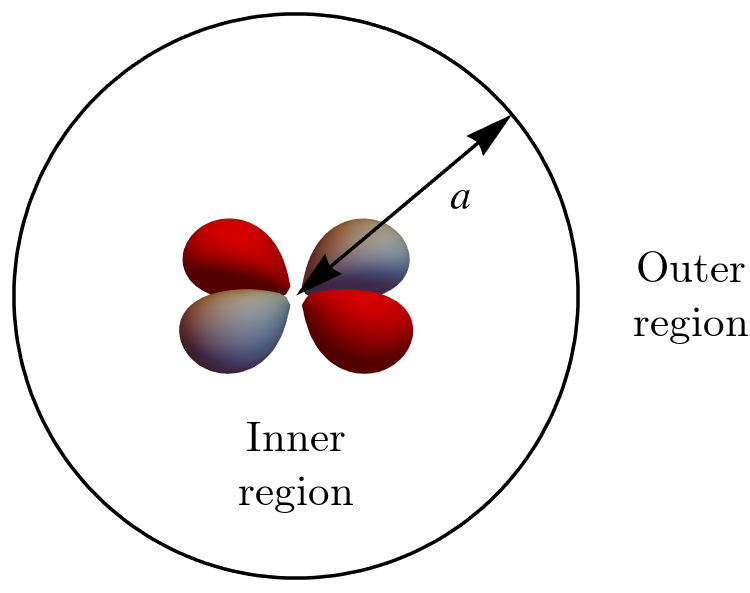
\includegraphics[scale=1]{2-ARM-theory/Figures/figure2E.png}
  \caption[$R$-matrix splitting of space]{$R$-matrix splitting of space into an inner spherical region of radius $a$ and an outer region outside that sphere.}
  \label{fig:2A-splitting-space}
\end{figure}

The Analytical $R$-Matrix method makes use of this spatial separation, not to implement different numerical methods on the two different regions, but rather to use different approximate analytical methods in their regions of validity. In particular, the solutions of the Schrödinger equation driven by the laser field -- the Volkov states we visited in the Introduction -- can be augmented to include the effect of the interaction with the parent ion through the eikonal-Volkov approximation~\cite{eikonalVolkov_initial, eikonalVolkov_prelim}, but this breaks down near the ion, so that solution needs to be fenced off from its singularities, where the normal atomic or molecular eigenstates can be used. Having done this, multi-electronic effects can then be built in by taking a single electron to be in the outer region and using the eigenstates of the ion as a basis, to which the outer electron is correlated.





In this chapter, we will show how these tools are built and come together to produce the theory: the separation of space, the different ingredient solutions, their integration, the encapsulation of the effect of the inner wavefunction on the outer one, and the use of the saddle-point approximation to produce clear physical pictures for the process.





\section{Basic framework}
\label{sec:basic-framework}

\subsection{Splitting space}


The separation of space into two parts, while conceptually simple, does pose some technical challenges that need to be addressed with the right language. Naively, we have an initial Hilbert space which describes wavefunctions over the whole of space,
\begin{equation}
\hil=\{\psi:\mathbb R^3\to \mathbb C \mid \int|\psi(\vbr)|^2 \d\vbr < \infty \}
\end{equation}
%
\begin{subequations}
%
and we want to separate it into functions from inside and outside the ball $B(a)$ of radius~$a$, 
\begin{align}
\hil_< & =\{\psi:B(a)\to \mathbb C \mid \int|\psi(\vbr)|^2 \d\vbr < \infty \} \\
\hil_> & =\{\psi:\mathbb R^3\setminus B(a)\to \mathbb C \mid \int|\psi(\vbr)|^2 \d\vbr < \infty \},
\end{align}
%
\end{subequations}
%
using the projectors $\Pi_\lessgtr:\hil \to \hil_\lessgtr$. We want to deal with the projected wavefunctions $\,\Pi_\lessgtr\! \ket\psi$ separately, so we simply project the Schrödinger equation as $i\frac{\d}{\d t} \,\Pi_\lessgtr\! \ket\psi=\,\Pi_\lessgtr  H \ket\psi$, and we reformulate it in terms of the projected wavefunctions. 

The technique is most easily illustrated, for simplicity, in one dimension (though of course it extends directly to the radius in three dimensions. Concentrating for the moment on the outer region, we're interested in the evolution of $\Pi_>\ket{\psi}$, which is given by
\begin{equation}
i\frac{\d}{\d t}\Pi_>\ket{\psi} 
= \Pi_> \,H\! \ket{\psi}
= H \,\Pi_> \!\ket{\psi} + \left[\Pi_>, \tfrac12\hat{p}^2\right]\ket{\psi},
\end{equation}
since the kinetic energy $\tfrac12\hat{p}^2$ does not commute with the spatial projection. To find the commutator $\left[\Pi_>, \tfrac12\hat{p}^2\right]$ that appears in the time evolution, the quickest route is to set $\Pi_> = \theta(\hat x-a)$, and to use the canonical commutation relation in the form
\begin{equation}
\hat{p} f(\hat{x}) = f(\hat{x}) \hat{p} -i f'(\hat{x}).
\end{equation}

Thus, we look at
\begin{align}
\hat{p}^2 \theta(\hat{x}-a)
& = 
\hat{p} \left( \theta(\hat{x}-a) \hat{p} - i \theta'(\hat{x}-a)\right)
\nonumber \\ & =
 -i\hat{p}\delta(\hat{x}-a)
 + \left(\theta(\hat{x}-a) \hat{p} - i \theta'(\hat{x}-a)\right)\hat{p}
\nonumber \\ & =
 -\left(i\hat{p}\delta(\hat{x}-a) + \delta(\hat{x}-a)i\hat{p} \right) 
 + \theta(\hat{x}-a)\hat{p}^2,
\end{align}
which then gives us the commutator as
\begin{equation}
\left[ \theta(\hat{x}-a),\hat{p}^2\right] = i\hat{p}\delta(\hat{x}-a) + \delta(\hat{x}-a)i\hat{p},
\end{equation}
and which we encapsulate using the notation
\begin{equation}
\hat{L}_0 \colonequals
\left[ \theta(\hat{x}-a),\tfrac12\hat{p}^2\right] = \frac{ i\hat{p}\delta(\hat{x}-a) + \delta(\hat{x}-a)i\hat{p}}{2},
\end{equation}
which is known as the Bloch operator, after Claude Bloch~\cite{ Bloch_L_operator_1957}.


With this commutator ready, the Schrödinger equation for the outside component~reads
\begin{equation}
i\frac{\d}{\d t} \theta(\hat{x}-a) \ket{\psi} 
= H \theta(\hat{x}-a)\ket{\psi} + \hat{L}_0\ket{\psi},
\end{equation}
%
\begin{subequations}
%
which we can further split into
\begin{equation}
i\frac{\d}{\d t} \theta(\hat{x}-a) \ket{\psi} 
= \left[ H + \hat{L}_0 \right] \theta(\hat{x}-a)\ket{\psi} + \hat{L}_0\theta(a-\hat{x})\ket{\psi}.
\end{equation}
Similarly, there is an identical equation for the inner wavefunction,
\begin{equation}
i\frac{\d}{\d t} \theta(a-\hat{x}) \ket{\psi} 
= \left[ H - \hat{L}_0 \right] \theta(a-\hat{x})\ket{\psi} - \hat{L}_0\theta(\hat{x}-a)\ket{\psi},
\end{equation}
%
\end{subequations}
%
and the two make up a pair of coupled inhomogeneous Schrödinger equations: each is governed by its own hamiltonian, altered with the addition of a Bloch operator to keep the per-component hamiltonian hermitian, and with coupled source terms $\pm\hat{L}_0 \theta(\mp(\hat{x}-a))\ket{\psi}$ that give the flow of probability from either region into the other.

In general, the coupled Schrödinger equations for the inner and outer regions are usually fine-tuned by the addition of a separate hermitian factor, to make the full Bloch operator read
\begin{equation}
L^{(\pm)}(a) = \pm \hat{L}_0 \pm \delta(\hat{x}-a)b(\hat{x}).
\label{e2-bloch-operator-with-function}
\end{equation}
%
\begin{subequations}
%
Ultimately we will choose $b(r) = (1-b)/r$, where $b$ is a constant, as it will significantly simplify the algebra, but for now we leave it arbitrary, and obtain our coupled Schrödinger equations in useful form:
\begin{empheq}[left=\empheqlbrace]{align}
i\frac{\d}{\d t}\ket{\psi_>} 
&= \left[ H - L^{(-)}(a) \right] \ket{\psi_>} - L^{(-)}(a) \ket{\psi_<},
\\
i\frac{\d}{\d t}\ket{\psi_<} 
&= \left[ H  - L^{(+)}(a) \right] \ket{\psi_<} - L^{(+)}(a)\ket{\psi_>}.
\end{empheq}
\end{subequations}


When solving these equations numerically, one usually keeps close track of both hamiltonians and both flow operators, and indeed in principle one can implement a full recollision step in ARM theory by using the in-flow from the outer region into the inner one, though this is as yet unexplored. For our purposes, however, it will be sufficient to look at the evolution of the outer region, and keep the inner-region wavefunction at the ground state of the neutral, essentially unperturbed, so $\ket{\psi_<}\approx \ket{\Psi_g}$, and this will work as our source term for the outer region.


We arrive, then, at the problem to be solved:
\begin{subequations}
\label{e2-problem}
\begin{align}
i\frac{\d}{\d t}\ket{\Psi(t)}
&=\left[H - \hat{L}^{(-)}(a)\right]\ket{\Psi(t)} -\hat{L}^{(-)}(a)\ket{\Psi_g}\!,
\\
\ket{\Psi(0)}&=\ket{\Psi_g}.
\end{align}
\end{subequations}
This problem can be solved formally, if one has access to the full propagator $U(t,t')$ corresponding to the $N$-electron hamiltonian $H$, satisfying $i\partial_t U(t,t') = H(t) U(t,t')$ under $U(t',t')=\id$, in which case the solution obeys
\begin{equation}
\ket{\Psi(t)}=-i\int_{-\infty}^t \!\d t' \, U(t,t')\hat{L}^{(-)}(a)\ket{\Psi_g(t')}.
\label{e2-formal-solution}
\end{equation}
Here we will take the state $\ket{\Psi(t)}$ inside the integral to be the neutral's ground state $\ket{\Psi_g}$, with ionization potential $I_p$ and energy $E_g=-I_p$: $\ket{\Psi_g(t)}= e^{+iI_p t}\ket{\Psi_g}$. This is the solution of the Schrödinger equation for the inner region obtained by ignoring backflow from the outer region and polarization of the neutral by the laser field; both of these effects can be reinstated later if required. As such, equation~\eqref{e2-formal-solution} represents a concrete Ansatz for the wavefunction we are looking for, and the problem now becomes that of obtaining suitable approximations for the propagator $U(t,t')$.




\subsection{The hamiltonian}
We wish to consider ionization of an atom or molecule by a strong, long-wavelength laser field, and we want to consider -- at least in the outer-region -- multi-electron effects. As such, the hamiltonian for the problem includes electrostatic forces for $N$ electrons, with nuclei of charge $Z_m$ at $\vb R_m$, and their length-gauge interaction with an external laser field~$\vb F(t)$:
\begin{subequations}
\label{e2-totalhamiltonian}
\begin{align}
H^N&=T_e^N+V_C^N+V_{ee}^N+V_L^N,\textrm{ where}\\
V_C^N&=-\sum_m \sum_{i=1}^N \frac{Z_m}{\|\vb{R}_m-\vb{r}_i\|},\\
V_{ee}^N&=\sum_{i>j}^N \frac{1}{\|\vbr_i-\vbr_j\|},\label{e2-V-ee-definition}\\
V_L^N&=\sum_{i=1}^N \vbf(t)\cdot \vbr_i.
\end{align}
\end{subequations}

Once the ionized electron leaves the molecule, the total hamiltonian is split into the $N-1$-electron ionic hamiltonian $H^{N-1}$, formally identical to the neutral one, and the hamiltonian for the leaving electron,
\begin{equation}
H_e\colonequals H^N-H^{N-1}
\end{equation}
which in particular contains the entangling operator $V_{ee}=V_{ee}^N-V_{ee}^{N-1}=\sum_{i=1}^{N-1}\|\vbr_i-\vbr\|^{-1}$, the Coulomb repulsion between the leaving electron and the ion. 

This hamiltonian can therefore be split into three specific components: the ionic core electrons in the inner region and their polarization by the laser field, the ionized electron and its strong driving in the outer region by the laser field, and their entangling interaction. We will add the entangling interaction in perturbatively, after developing approximate analytical propagators for each factor.



\subsection{Eikonal-Volkov states}
We begin by focusing on the ionized electron, which will be driven by a hamiltonian of the form
\begin{equation}
H_e=\frac12 \hat{\vbp}^2 + \vbf(t)\cdot\hat\vbr + V(\vbr),
\label{e2-single-electron-hamiltonian}
\end{equation}
where $V(\vbr)$ is an electrostatic interaction with the ionic core, and which is considered weak in the outer region. If one ignores this electrostatic interaction, leaving the laser-driven hamiltonian $H_L=\frac12 \hat{\vbp}^2 + \vbf(t)\cdot \hat\vbr$, the Schrödinger equation has well-known exact solutions known as Volkov states~\cite{ bergou_volkov_sates_1980}, as we met them earlier in \eqref{e1-volkov-wavefunctions},
\begin{align}
\phantom{{}^\mathrm{EA}}
\braket{\vb{r}}{\vb{k}^{\mathrm{(V)}}(t)}
& = 
\frac{1}{(2\pi)^{3/2}}
e^{i\left(\vb{k}+\vba(t)\right)\cdot\vb{r}} 
e^{-\frac{i}{2} \int_T^t\left(\vb{k}+\vba(\tau)\right)^2\d\tau},
\phantom{e^{-i\int_T^t U_n(\rl(\tau;\vb{r},\vb{k},t),\tau)\d\tau}}
\label{e2-volkov-wavefunctions}
\end{align}
defined in terms of the vector potential of the field $\vba(t)$, which must obey $\vbf(t) = -\frac{\d\vba}{\d t}$.

To include the interaction with the electrostatic potential $V(\vbr)$, we use the eikonal-Volkov approximation~\cite{eikonalVolkov_initial, eikonalVolkov_prelim}, which is an adaptation of the Wentzel-Kramers-Brillouin (WKB) method to the $V(\vbr)$-driven interaction-picture Schrödinger equation on top of the Volkov states of \eqref{e2-volkov-wavefunctions}: one posits a wavefunction modified by an amplitude and a phase, and then solves perturbatively for both. The result are the wavefunctions
\begin{align}
\braket{\vb{r}}{\vb{k}^{\mathrm{(EVA)}}(t)}
& = 
\frac{1}{(2\pi)^{3/2}}
e^{i\left(\vb{k}+\vba(t)\right)\cdot\vb{r}} 
e^{-\frac{i}{2} \int_T^t\left(\vb{k}+\vba(\tau)\right)^2\d\tau} 
e^{-i\int_T^t V(\rl(\tau;\vb{r},\vb{k},t),\tau)\d\tau},
\label{e2-eikonal-volkov-wavefunctions}
\end{align}
with an added Coulomb phase $e^{-iW_C}=e^{-i\int_T^t V(\rl(\tau;\vb{r},\vb{k},t),\tau) \d\tau}$ in terms of the laser-driven trajectory
\begin{align}
\rl(\tau;\vb{r},\vb{k},t)
& \colonequals 
\vb{r}+\int_t^\tau \left[\vb{k}+\vba(\tau')\right]\d\tau'
\label{e2-trajectory}
\end{align}
that starts at position $\vbr$ at time $t$ and has asymptotic momentum $\vbk$. The eikonal-Volkov states are in general valid as long as the boundary radius $a$ is far enough from the ion.






\subsection{Ionic states}
In addition to the continuum wavefunctions, in going from a single-active-electron approach to a multi-channel one where the ionized electron is entangled with the ionic core, we also require an appropriate basis of solutions for the different channels of the core. In particular, we want to solve the time-dependent Schrödinger equation in the inner region for the $N-1$ electrons of the ion, $i\partial_t\!\ket*{\Psi^{N-1}}=H^{N-1}\ket*{\Psi^{N-1}}$, potentially including polarization effects induced by the external field.

To solve this problem, we choose the basis of instantaneous eigenstates of the ion, which obey
\begin{equation}
H^{N-1}(t)\ket{n(t)}=E_n(t)\ket{n(t)}
\label{e2-quasistatic-eigenstates}
\end{equation}
at each instant $t$, and from which one can construct approximate TDSE solutions of the form 
$e^{-i\int^tE_n(\tau)\d \tau}\ket{n(t)}$ as long as the laser frequency $\omega$ is smaller than the characteristic energy spacing $\Delta E$ of the system.

In practice, this thesis will not address such polarization effects, but they can be included if required, by diagonalizing the field hamiltonian on a constrained basis of atomic or molecular eigenstates using their transition dipole moments as their interaction with the field. It is interesting to note that when including polarization effects this approach does extend to the complex-time formalism we will pursue later to apply the saddle-point approximation to temporal integrals, but this is not a trivial step: the real-time instantaneous eigenstates of \eqref{e2-quasistatic-eigenstates} do extend into the complex plane as analytic functions~\cite{hwang_adiabatic_1977, pechukas_analytic_1976}, but in general they will develop branch points at complex times $t^*$ where pairs of eigenvalues become degenerate. One can then extract rich structure from these analytical functions -- including, among others, the Landau-Dykhne nonadiabatic transition rate between the different states~\cite{dykhne_adiabatic_1962, hwang_adiabatic_1977}.


For now, though, we can use the instantaneous eigenstates to extract the electrostatic potential to be used for the eikonal-Volkov states, given by the self-consistent field
\begin{equation}
U_n(\vb{r})\colonequals \bra{n(t)}\otimes\bra{\vb{r}}V_{ee}\ket{n(t)}\otimes\ket{\vb{r}}.
\label{e2-channel-specific-potential}
\end{equation}
With this choice of potential for $V(\vbr)$, the eikonal-Volkov states satisfy the Schrödinger equation
\begin{equation}
i\partial_t\ket{\vb{k}_n(t)}=H_e^n(t)\ket{\vb{k}_n(t)}
\qq{for}
H_e^n\colonequals \matrixel{n(t)}{H^N-H^{N-1}}{n(t)}.
\label{e2-channel-specific-eikonal-tdse}
\end{equation}
There is, of course, an additional entangling component of $V_{ee}$ that goes beyond this self-consistent part, and that will be dealt with separately as the potential driving the channel mixing.

Finally, we can put together the instantaneous eigenstates and the eikonal-Volkov states to get an appropriate resolution of identity,
\begin{align}
1=\int\d\vb{k}\sum_n
\mathbb{A}\ket{\vb{k}_n(t)}\otimes\ket{n(t)}\bra{\vb{k}_n(t)}\otimes\bra{n(t)}\mathbb{A}
\label{e2-resolutionofidentity}
\end{align}
where $\mathbb{A}$ is the anti-symmetrizing operator, which when applied to our formal solution \eqref{e2-formal-solution} gives us an equation,
\begin{align}
\ket{\Psi(t)}
= -i\sum_n\int\d\vb{k}\int_{-\infty}^t  &  \d t' \, U^N(t,t')\mathbb{A}\ket{n(t')}\otimes\ket{\vb{k}_n(t')}
\nonumber \\ & \qquad   \times \bra{\vb{k}_n(t')}\otimes\bra{n(t')}\mathbb{A}\hat{L}^{(-)}(a)\ket{\Psi_g}e^{iI_p t'},
\label{e2-channel-specific-formal-solution}
\end{align}
that is ready for further work.



\subsection{The Dyson orbital}
To tackle our channel-specific formal solution \eqref{e2-channel-specific-formal-solution}, we begin with the transition matrix element of the Bloch operator,
\begin{equation}
\bra{\vb{k}_n(t')}\otimes\bra{n(t')}\mathbb{A}\hat{L}^{(-)}(a)\ket{\Psi_g}.
\end{equation}
This expression hides two summations over the different electrons: one over which electronic Bloch operator acts on $\ket{\Psi_g}$, and one, induced by the anti-symmetrizing $\mathbb{A}$, over which electron is induced into the continuum state $\ket{\vb{k}_n(t')}$. 

We can, however, neglect the contribution from the non-diagonal, exchange-like terms, in which an electron different from the one transmitted by the Bloch operator to the outer region is projected into the continuum state. In terms of the characteristic momentum $\kappa$ of the ground state, with $\frac{1}{2}\kappa^2=I_p$, this can be ensured as long as $\kappa a\gg 1$. This effectively breaks the exchange symmetry -- which is fundamentally due to the fact that in the outer region the ionized electron is distinguishable from those left behind -- and allows us to choose which electron will tunnel out into the continuum state; this reduces the matrix element to 
\begin{equation}
\bra{\vb{k}_n(t')}\otimes\bra{n(t')}\mathbb{A}\hat{L}^{(-)}(a)\ket{\Psi_g}=\frac{N}{\sqrt{N}}\bra{\vb{k}_n(t')}\hat{L}^{(-)}(a)\cdot \braket{n(t')}{\Psi_g},
\end{equation}
where we include normalization factors of $\frac{1}{\sqrt{N}}$, due to the normalization of $\mathbb{A}$, and $N$, due to the different electrons the Bloch operator can act on. From here on we revert the Bloch symbol $\hat{L}^{(-)}(a)$ to a single-electron operator as originally introduced.

The remaining single-electron wavefunction on the right of the Bloch operator can now be recognised to be the Dyson orbital corresponding to channel $n$, which we denote by
%%%%%
%%\pdfmargincomment{Reference for Dyson orbital missing.}
%%%%%
\begin{equation}
\ket{n_{D}(t)}=\sqrt{N}\braket{n(t)}{\Psi_g}.
\label{e2-dysonorbital}
\end{equation}
The matrix element in question is then left as
\begin{equation}
\bra{\vb{k}_n(t')}\otimes\bra{n(t')}\mathbb{A}\hat{L}^{(-)}(a)\ket{\Psi_g}
=
\bra{\vb{k}_n(t')}\hat{L}^{(-)}(a)\ket{n_D(t')}.
\end{equation}
Finally, we note that the above is also valid in the single-electron case, provided that one drops the ion states and simply takes the Dyson orbital to be the ground state.




\subsection{Separating the single- and cross-channel amplitudes}
We now turn to the propagator part of \eqref{e2-channel-specific-formal-solution} -- the terms in $U^N(t,t')\mathbb{A}\ket{n(t')}\otimes\ket{\vb{k}_n(t')}$ that take the electron, ionized at $t'$ with amplitude $\bra{\vb{k}_n(t')}\hat{L}^{(-)}(a)\ket{n_D(t')}$ as above, to its state at time $t$. Our chosen basis enables us to propagate the ionic state $\ket{n(t)}$ and its corresponding eikonal-Volkov continuum state $\ket{\vb{k}_n(t)}$, on the level of the self-consistent field $U_n(\vbr)$ of the ion, but we have yet to account for the entangling part of the interaction,
\begin{equation}
V_{ee}^n(t)\colonequals V_{ee}-\bra{n(t)}V_{ee}\ket{n(t)},
\label{e2-correlation-interaction-potential}
\end{equation}
in terms of which the total hamiltonian can be written as
\begin{equation}
H^{(-)}=H^{N-1}+H_e^n(t)+V_{ee}^n(t).
\end{equation}
%%%
%%%  Should the first H be curly?
%%%

We deal with this combination in a perturbative fashion with respect to the entangling interaction, treating the correlation operator $V_{ee}^n$ as a small effect on top of the single-active electron dynamics of tunnel ionization. We use, specifically, the main tool of time-dependent perturbation theory, the Dyson expansion.


\begin{mathaside}{The Dyson expansion}
\label{aside.dyson-expansion}
\noindent
Suppose that the total hamiltonian of the system is split as $H=H_0+\Delta H$ between a basic hamiltonian $H_0$ whose propagator $U_0(t,t')$ is known, solving 
\begin{equation}
i\frac{\partial}{\partial t} U_0(t,t')=H_0U_0(t,t')\textrm{  under  }U_0(t,t)=1,
\end{equation}
and an additional interaction $\Delta H$. Then the full propagator $U(t,t')$ for $H$, satisfying
\begin{equation}
i\frac{\partial}{\partial t} U(t,t')=HU(t,t')\textrm{  under  }U(t,t)=1,
\end{equation}
can be written recursively in the form 
\begin{equation}
U(t,t')=-i\int_{t'}^t \d t'' \, U(t,t'') \Delta H(t'') U_0(t'',t')+U_0(t,t').
\label{e2-dyson-expansion}
\end{equation}
Repeated application of this expansion gives a series solution for $U(t,t')$ in powers of $\Delta H$, though this series need not converge and may require renormalization procedures to work well~\cite{fetter_walecka}. A proof of this identity, via direct calculation, is available in~\citer{ MResReport}.
\end{mathaside}


Applying this expansion to our split of the hamiltonian on each of the channels, and treating the channel-specific correlation operator $V_{ee}^n$ as the perturbation, enables us to write our wavefunction as a direct contribution and a cross-channel one, 
\begin{subequations}
\label{e2-first-decomposition}
\begin{equation}
\ket{\Psi(t)}=\ket*{\Psi^{(0)}(t)}+\ket*{\Psi^{(1)}(t)}
\label{e2-decomposition}
\end{equation}
where in the direct channel the ionized electron is distinguishable, so the antisymmetrizer drops out and the propagator separates into the ionic propagator $U^{N-1}(t,t')$ and the channel-specific continuum propagator $U_e^n(t,t')$,
\begin{align}
\ket{\Psi^{(0)}(t)}=-i\sum_n \int\d\vb{k}\int^t\d t' & U^{N-1}(t,t')\ket{n(t')} \otimes U_e^n(t,t')\ket{\vb{k}_n(t')}
\nonumber \\ & \times
\matrixel{\vb{k}_n(t')}{\hat{L}^{(-)}(a)}{n_D(t')}e^{iI_p t'}
\label{e2-abstract-direct-state}
\end{align}
and the cross-channel contribution is given by
\begin{align}
\ket{\Psi^{(1)}(t)}
=(-i)^2\sum_n  & \int\d\vb{k}\int^t\d t''\int^{t''}\d t'U^N(t,t'')V_{ee}^n(t'') U^{N-1}(t'',t')\ket{n(t')}
\nonumber \\ & \otimes 
U_e^n(t'',t')\ket{\vb{k}_n(t')}\times\matrixel{\vb{k}_n(t')}{\hat{L}^{(-)}(a)}{n_D(t')}e^{iI_p t'}.
\label{e2-abstract-correlation-state}
\end{align}
\end{subequations}






\section{The direct ionization amplitude}
\label{sec:direct-ionization-amplitude}
In this section we will focus on the direct tunnelling term, $\ket*{\Psi^{(0)}(t)}$, which accounts for the single-active electron dynamics that are of interest in chapters \ref{chap:quantum-orbits} and~\ref{chap:LES-NZES} of this thesis, and which form the baseline for the correlation-driven dynamics studied in chapter~\ref{chap:multi-channel}.

To bring the calculation down to more concrete quantities, we consider the ionization yield with final momentum $\vb{p}$ in channel $n$: that is, we want the probability amplitude for the ion to be left in the free state $\ket{n}$ with the ionized electron at canonical and mechanical momentum $\vbp$ at some time $T$ after the laser pulse has finished. 

In the cases where we're interested in the final state of the ion after the pulse is over, there is an additional complication in that the laser pulse may cause transitions among different quasi-static eigenstates of the ion between the ionization event and the end of the pulse, and to evaluate this we would require a prohibitively complex $(N-1)$-electron back-propagation of the Schrödinger equation.

To reach a compromise, we project on the basis of quasi-static eigenstates at a time $\tn$ shortly after the ionization step is completed. This is equivalent to projecting on the basis $U^{N-1}(T,\tn)\ket{n(\tn)}$ at time $T$ and represents a definite loss of contrast to projecting on the free states $\ket{n}$, but since the transitions caused by the laser are indistinguishable from those caused by the electron this loss of contrast is inevitable.

We therefore define the ionization yield, our main handle on the system's state, as
\begin{equation}
a_n(\vb{p},\tn)\colonequals\bra{\vb{p}}\otimes\bra{n(\tn)}U^{N-1}(\tn,T)\ket{\Psi(T)}\!.
\label{e2-ionization-yield}
\end{equation}
In these terms, the direct ionization yield corresponding to the first-order term of \eqref{e2-abstract-direct-state} is naturally given by
\begin{align}
a_m^{(0)}(\vb{p},\tn)
=
-i\sum_n \int_{-\infty}^{\tn}\!\d t' \matrixel{m(\tn)}{U^{N-1}(\tn,t')}{n(t')} \matrixel{\vb{p}_n(t')}{\hat{L}^{(-)}(a)}{n_D(t')}e^{iI_p t'},
\label{e2-setup-a1}
\end{align}
and it describes a single ionization burst centred at a time $\tn$.

Moreover, we now neglect the effects of polarization of the core, so the ionic eigenstates reduce to their free propagation,
\begin{equation}
\matrixel{m(\tn)}{U^{N-1}(\tn,t')}{n(t')}=\delta_{mn}e^{-iE_m(\tn-t')},
\label{e2-propagated-quasistatic-eigenstates}
\end{equation}
so the ionization yield reduces to
\begin{align}
a_n^{(0)}(\vb{p},\tn)
=
-i e^{-iE_n\tn} \int_{-\infty}^{\tn}\!\d t' \matrixel{\vb{p}_n(t')}{\hat{L}^{(-)}(a)}{n_D(t')}e^{i I_{p,n} t'},
\label{e2-sae-yield-beginning}
\end{align}
where 
\begin{equation}
I_{p,n}=E_n-E_g=I_p+E_n
\end{equation}
is the ionization potential into channel $n$.









\subsection{The Volkov action and its saddle-point approximation}
We now tackle the continuum state matrix element in the ionization yield of \eqref{e2-sae-yield-beginning}. This state, given in the position representation by \eqref{e2-eikonal-volkov-wavefunctions}, has two main ingredients, which play two distinct roles: the spatial plane-wave dependence $e^{i\left(\vb{k}+\vba(t)\right)\cdot\vb{r}}$, which in the matrix element $\matrixel{\vb{p}_n(t')}{\hat{L}^{(-)}(a)}{n_D(t')}$ extracts the relevant spatial information from the Dyson orbital and the ionizing Bloch operator, and the phase $e^{-\frac{i}{2} \int_T^t\left(\vbp+\vba(\tau)\right)^2\d\tau}$, which carries most of the strong time dependence in the integral in \eqref{e2-sae-yield-beginning}. 

We will now disentangle these two roles: we will encapsulate the spatial dependence into a single shape factor, and we will perform a saddle-point approximation to resolve the temporal integral into specific trajectory-based components. However, because the factor of $e^{i\vba(t)\cdot\vb{r}}$ weaves both the spatial and temporal integrals together, disentangling the two roles will require a certain amount of approximation.

To begin with, putting in the explicit eikonal-Volkov state into \eqref{e2-sae-yield-beginning}, via a decomposition of unity in the position representation, transforms it into
\begin{align}
a_n^{(0)}(\vb{p},\tn)
=
-i e^{-iE_n\tn} 
\int_{-\infty}^{\tn}\!\d t'
&  
e^{\frac{i}{2} \int_T^{t'}\left(\vbp+\vba(\tau)\right)^2\d\tau}
e^{i I_{p,n} t'}  
\int\frac{\d\vbr}{(2\pi)^{3/2}}
e^{-i\left(\vbp+\vba(t')\right)\cdot\vb{r}} 
\nonumber \\ & \qquad \times
e^{i\int_T^{t'} U_n(\rl(\tau;\vb{r},\vbp,t'),\tau)\d\tau}
\matrixel{\vbr}{\hat{L}^{(-)}(a)}{n_D(t')}.
\end{align}
For simplicity, the arguments of $U_n$ will hereafter be dropped unless they play an active role. Moreover, as before, we will neglect the contributions of polarization of the core, and ignore the time dependence of the Dyson orbital (and, similarly, in the mean-field electrostatic interaction $U_n$). This then lets us reorganize the integrals in the form
\begin{align}
a_n^{(0)}(\vb{p},\tn)
=
&  
-i e^{-iE_n\tn} 
\int\frac{\d\vbr}{(2\pi)^{3/2}}
\matrixel{\vbr}{\hat{L}^{(-)}(a)}{n_D}
\nonumber \\ &  \times
\int_{-\infty}^{\tn}\!\d t'
e^{-i\left(\vbp+\vba(t')\right)\cdot\vb{r}} 
e^{i I_{p,n} t'}  
e^{\frac{i}{2} \int_T^{t'}\left(\vbp+\vba(\tau)\right)^2\d\tau}
e^{i\int_T^{t'} U_n(\rl(\tau;\vb{r},\vbp,t'))\d\tau}
.
\label{e2-yield-after-order-switch}
\end{align}






The problem with this integral is that it is highly oscillatory, essentially through the influence of the terms $e^{i I_{p,n} t'} e^{\frac{i}{2} \int_T^{t'} \left(\vbp+ \vba(\tau) \right)^2\d\tau}$: the integrand changes sign with a frequency dictated by the ionization potential, via $e^{i I_{p,n} t'}$, but it is integrated over timescales of at least several laser cycles, with a laser frequency $\omega$ much smaller than $I_p$. The result is shown in \reffig{f2-oscillatory-factors}: a function which oscillates rapidly, with varying frequency. In general, the integral of such a function can indeed be calculated numerically -- most easily when\ an explicit oscillatory factor like $e^{i I_{p,n} t'}$ is present -- but calculating it accurately is challenging, because of the numerous cancellations: if $a$ and $b$ are very close to each other, one needs very high accuracy in both $a$ and $b$ to get even mediocre accuracy in $a-b$.


\newcommand{\figuretwoAtarget}{hydrogen}
\newcommand{\figuretwoAfield}{0.053}
\newcommand{\figuretwoAlambda}{800}
\newcommand{\figuretwoAmomentum}{0.5}%
\begin{figure}[htb]
  \centering
  $\Re\left[
  e^{i I_{p,n} t}e^{\frac{i}{2} \int_T^{t}\left(p+A(\tau)\right)^2\d\tau}
  \right]$\\[-3mm]
  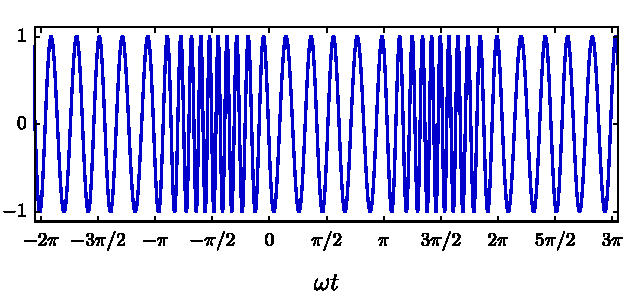
\includegraphics[scale=1]{2-ARM-theory/Figures/figure2A.pdf}
  \caption[Oscillatory factors of the SFA integrand prior to the saddle-point approximation]{%
  Real part of the oscillatory factors of Eq.~\eqref{e2-yield-after-order-switch}, for a sinusoidal field of the form $A(t)=-\frac{F}{\omega}\sin(\omega t)$.
  Here the field strength is $F=\SI{\figuretwoAfield}{\au}$, for a $\lambda= \SI{\figuretwoAlambda}{nm}$ field ionizing \figuretwoAtarget{} into a final momentum of $p=\SI{\figuretwoAmomentum}{\au}$
  }
  \label{f2-oscillatory-factors}
\end{figure}
%%% Note hackish a.u. - period interaction at the end there.


The solution is to use what is known as the \textit{saddle-point approximation}. If the integrand is an analytic function of $t'$, we can deform the path of integration to any path that connects the two endpoints and obtain the same integral, so we can look for better choices of integration contour. The basic features of the integrand are captured mainly by the oscillatory factors, $e^{i I_{p,n} t'} e^{\frac{i}{2} \int_T^{t'} \left(\vbp+ \vba(\tau) \right)^2\d\tau}=e^{-iS(t')}$, whose structure is shown in \reffig{f2-saddle-points-3d}. 

\begin{figure}[t!]
  \centering
  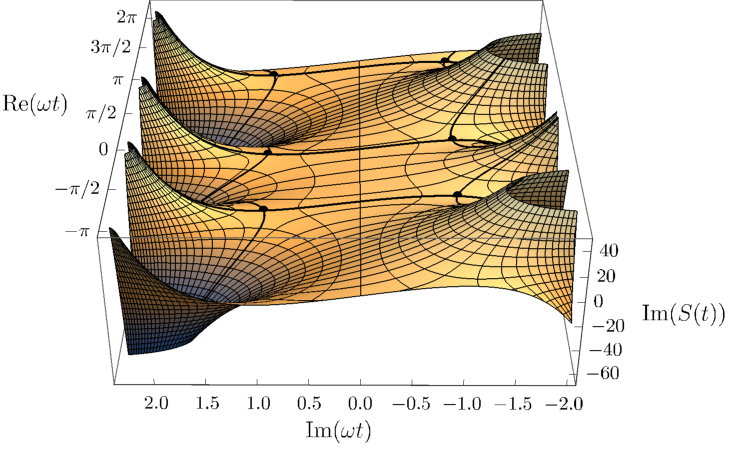
\includegraphics[scale=1]{2-ARM-theory/Figures/figure2B.pdf}
  \caption[Landscape of the imaginary action $\Im(S(t))$ over imaginary time, showing the steepest-descent contours]{%
    Landscape for the amplitude of the exponent in the oscillatory factors, $e^{-iS(t')}=e^{i I_p t'} e^{\frac{i}{2} \int_T^{t'} \left(p+ A(\tau) \right)^2\d\tau}$, for the same field as \reffig{f2-oscillatory-factors}. The height and colour of the landscape indicate $\Im(S(t'))$, which governs the amplitude of the integrand through $|e^{-iS(t')}|=e^{\Im{S(t')}}$. The lines of constant $\Re(S(t'))$ are orthogonal to the $\Im(S(t'))$ contour lines, and they form the paths of steepest ascent and descent on the landscape, along which $e^{-iS(t')}$ ceases to oscillate, changing only in amplitude.
  }
  \label{f2-saddle-points-3d}
\end{figure}


In particular, if we shift the contour towards positive imaginary times, the amplitude of the oscillations, given by $|e^{-iS(t')}|=e^{\Im\left(S(t')\right)}$ decreases sharply except for a few points of maximal contribution, and if we make the contour pass through the saddle points of the landscape (the solutions of the complex equation $\frac{\d S(t')}{\d t'}=0$), we minimize the maximal amplitude of the integrals. In addition to this, we can also choose an integration contour along the lines where the $\Re(S(t'))$ is constant, which guarantees that the amplitude drop is as fast as possible and that the oscillations stop; the integrand $e^{-iS(t')}$ then becomes a series of sharp, flat, gaussian-like humps centred on each of the saddles. 

So far, this procedure can be done exactly, and it provides a way to neutralize the effect of the integrand's oscillations at the cost of finding a complicated contour and integrating over it. The saddle-point approximation itself consists of forgetting about the long tails of the contour in the valleys of the integrand, and seeing the transformed integrand for what it is: a series of humps which are very well approximated by gaussians that can be integrated exactly, leaving a single contribution from each hump.


\pagebreak
\begin{mathaside}{The saddle-point approximation}
\label{aside.SPA}
\noindent
More precisely, if $F$ is an analytic function which varies slowly with respect to the analytic exponent $\varphi$, then the integral of the combination $e^{\rho \varphi(\zeta)}$ can be approximated by a sum of the form
\begin{equation}
\int_A^B F(\zeta) e^{\rho \varphi(\zeta)}\d\zeta
=
\sum_s
\sqrt{\frac{2\pi}{\rho}} 
\frac{F(\zeta_s) e^{\rho\varphi(\zeta_s)}}{\left[-\varphi''(\zeta_s)\right]^{1/2}}
\label{e2-SPA-statement}
\end{equation}
over all the relevant saddle points $\zeta_s$, which satisfy $\varphi'(\zeta_s)=0$ and are accessible to a deformed contour that joins $A$ and $B$~\cite{BruijnAsymptotics, Bleistein_Integrals, GerlachSPAonline}. In general this approximation holds in an asymptotic sense as the multiplier increases to $\rho\to\infty$, which is missing from our exponent, but in practice the exponent is large enough that the saddle-point approximation is excellent.
\end{mathaside}




Turning back to our integral, we see that the temporal integral 
\begin{align}
\int_{-\infty}^{\tn}\!\d t'
e^{-i\left(\vbp+\vba(t')\right)\cdot\vb{r}
 +i I_{p,n} t'
 +\frac{i}{2} \int_T^{t'}\left(\vbp+\vba(\tau)\right)^2\d\tau}
e^{i\int_T^{t'} U_n(\rl(\tau;\vb{r},\vbp,t'))\d\tau}
\label{e2-temporal-integral-before-saddle-point}
\end{align}
naturally splits into two components: a slow-acting Coulomb phase $e^{i\int_T^{t'} U_n(\rl(\tau;\vb{r},\vbp,t'))\d\tau}$ and a fast oscillatory factor $e^{-iS_V(t')}$ where the phase is given by the classical action of an electron in the field, 
\begin{equation}
S_V(t')
=
\left(\vbp+\vba(t')\right)\cdot\vb{r}
-I_{p,n} t'
-\frac{1}{2} \int_T^{t'}\left(\vbp+\vba(\tau)\right)^2\d\tau,
\label{e2-volkov-action-definition}
\end{equation}
which we will generally call the Volkov action.

The saddle-point approximation then asks us to look for the points at which this phase is stationary, which happens when
\begin{align}
0 & =
\frac{\d S_V}{\d t'}(\tvr)
=
\frac{\d}{\d t'}\left[-\frac{1}{2} \int_T^{t'}\left(\vbp+\vba(\tau)\right)^2\d\tau- I_{p,n} t'+\left(\vbp+\vba(t')\right)\cdot\vb{r}\right]_{\tvr}
\nonumber \\ & = 
-\left(\frac{1}{2} \left(\vbp+\vba(\tvr)\right)^2+ I_{p,n} + \vbf(\tvr)\cdot\vbr\right)
.
\end{align}
This condition is relatively complicated, because the equation, and therefore also the solution,~$\tvr$, depends on the position $\vbr$, which will later be integrated over. To tackle this, we will concentrate on a `central' saddle point, which satisfies the equation
\begin{equation}
\frac{1}{2} \left(\vbp+\vba(\ts)\right)^2+ I_{p,n}=0,
\label{e2-ts-equation}
\end{equation}
and then we will estimate the effect of the additional terms $\vbf(\tvr)\cdot\vbr$ on~$\tvr$. In general, if the boundary radius is chosen well inside the tunnelling region, which occurs when
\begin{equation}
|Fa|\ll I_{p,n},
\label{e2-Fa-Ip-restriction}
\end{equation}
then $\tvr$ will be close to $\ts$ and we will be able to estimate the effect of the term $\vbf(\tvr)\cdot\vbr$ in a linearized regime.


For the monochromatic, linearly polarized fields we consider, the saddle-point equation \eqref{e2-ts-equation} is easy to solve. Separating the momentum into its parallel and orthogonal components with respect to the laser polarization, and taking 
\begin{equation}
\vba(t)=-\frac{F}{\omega}\un \sin(\omega t),
\label{e2-field-definition}
\end{equation}
the saddle-point equation reads
\begin{equation}
\frac{1}{2} \left(\pp -\frac{F}{\omega}\sin(\omega \ts) \right)^2 +\frac{1}{2}\pt^2 + \frac 12 \kappa_n^2=0,
\end{equation}
for $\kappa_n=\sqrt{2I_{p,n}}$, or, alternatively,
\begin{equation}
\pp -\frac{F}{\omega}\sin(\omega \ts)
=\pm\sqrt{-(\kappa_n^2+\pt^2)},
\end{equation}
which is easily resolved to 
\begin{equation}
\omega \ts
= \arcsin\left(
\frac{\omega}{F}\left(\pp\pm i \sqrt{\kappa_n^2+\pt^2}\right)
\right).
\end{equation}
Here the arcsine function is a standard holomorphic function \citenistsec{4.23}, whose principal branch has branch cuts on $(-\infty,-1]$ and $[1,\infty)$, and takes values in the complex strip $-\frac{\pi}{2}<\Re(\arcsin(\zeta))<\frac{\pi}{2}$. In particular, the arcsine function takes the upper half-plane $\Im(\zeta)>0$ into the upper half-strip $\Im(\arcsin(\zeta))>0$, and since we're only interested in saddle-point times $\ts$ with positive imaginary parts -- as those are the ones that give acceptable contours, as shown in \reffig{f2-oscillatory-factors} -- we can finally take only the positive sign to~get
\begin{equation}
\omega \ts
= \arcsin\left(
\frac{\omega}{F}\left(\pp + i \sqrt{\kappa_n^2+\pt^2}\right)
\right).
\label{e2-saddle-point-equation-final-solution}
\end{equation}


To solve the full equation for $\tvr=\ts+\Delta \tvr$, we linearize the equation at $\ts$, which reads
\begin{equation}
\vba(\tvr)
=\vba(\ts +\Delta\tvr)
\approx \vba(\ts) + \Delta\tvr\frac{\d\vba}{\d t}(\ts)
=\vba(\ts) - \Delta\tvr \vbf(\ts)
\end{equation}
and a similar expansion for $\vbf(\tvr)$, to get 
\begin{align}
0
& = 
\frac{1}{2} \left(\vbp+\vba(\ts)-\Delta t_a\vbf(\ts)\right)^2+ I_{p,n} + \vbf(\ts)\cdot\vbr +\Delta t_a\frac{\d\vbf}{\d t}(\ts)\cdot\vbr 
\nonumber \\ & = 
\frac{1}{2} \left(\vbp+\vba(\ts)\right)^2+ I_{p,n}  -\Delta t_a\left(\vbp+\vba (\ts) \right) \cdot\vbf(\ts) + \vbf(\ts)\cdot\vbr 
\nonumber \\   & \qquad+
\frac{1}{2} \left(\Delta t_a\vbf(\ts)\right)^2  +\Delta t_a\frac{\d\vbf}{\d t}(\ts)\cdot\vbr
\nonumber \\ & = 
\Delta t_a\left(\frac{\d\vbf}{\d t}(\ts)\cdot\vbr-\left(\vbp+\vba(\ts)\right)\cdot\vbf(\ts) \right) + \vbf(\ts)\cdot\vbr 
%\nonumber \\   & \qquad+
+\frac{1}{2} \left(\Delta t_a\vbf(\ts)\right)^2 
.
\end{align}
Dropping the quadratic term for consistency, we get $\Delta\tvr$ in the form
\begin{equation}
\Delta\tvr
= \frac{\vbr\cdot\vbf(\ts)}{\left(\vbp+\vb{A}(\ts)\right)\cdot\vbf(\ts)}
=\frac{z}{\pp+A(\ts)},
\end{equation}
where $z=\vbr\cdot\un$ is the position coordinate along the laser polarization. Here, we should note that the denominator in this expression, $\pp+A(\ts)$, gives the kinematic momentum -- equal to the velocity $\vp(\ts)$, since the mass is unity -- at the time of ionization $\ts$. Moreover, this kinematic momentum is completely determined by the saddle-point equation \eqref{e2-saddle-point-equation-final-solution},~as 
\begin{equation}
\vp(\ts)=\pp+A(\ts)=-i\sqrt{ \kappa_n^2+\pt^2} \approx -i\kappa_n.
\label{e2-vp-as-i-kappa}
\end{equation}
Finally, the position $z=\vbr\cdot\un$ in the numerator is bounded, since the $\vbr$ integral is to be taken only over the ARM boundary of radius $a$.


We can now begin using these tools to simplify our integral, which with the application of the saddle-point approximation reads
\begin{align}
& a_n^{(0)}(\vb{p},\tn)
 =
-i e^{-iE_n\tn} 
\int\frac{\d\vbr}{(2\pi)^{3/2}}
\matrixel{\vbr}{\hat{L}^{(-)}(a)}{n_D}
\int_{-\infty}^{\tn}\!\d t'
e^{-iS_V(t')}
e^{i\int_T^{t'} U_n(\rl(\tau;\vb{r},\vbp,t'))\d\tau}
\nonumber \\ & \qquad \approx 
-i e^{-iE_n\tn} 
\int\frac{\d\vbr}{(2\pi)^{3/2}}
\matrixel{\vbr}{\hat{L}^{(-)}(a)}{n_D}
\sqrt{\frac{2\pi}{iS_V''(\tvr)}}
e^{-iS_V(\tvr)}
e^{i\int_T^{\tvr} U_n(\rl(\tau;\vb{r},\vbp,\tvr))\d\tau}
.
\label{e2-yield-after-saddle-point-approximation}
\end{align}
Here it is important to note that we are focusing on the contribution from a \textit{single} burst of ionization, represented by the selection of the contribution of a single saddle point. To get the full contribution, one must select all relevant saddle points and add their contributions coherently, which then gives rise to both inter-cycle interference -- otherwise known as ATI rings -- and intra-cycle interferences which provide additional structure to the photoelectron spectrum. In this thesis, however, we will focus on the details of the contribution of each specific ionization burst.


For now, we focus on analysing the contribution of the phase $e^{-iS_V(\tvr)}$, which we can again linearize with respect to the saddle point displacement $\Delta\tvr$ to get
\begin{align}
S_V(\tvr) & =S_V(\ts) + \Delta\tvr S_V'(\ts)
\\ \text{with}\quad
S_V'(\ts) & =
\frac{\d\vba}{\d t}(\ts)\cdot\vbr
-I_{p,n}
-\frac{1}{2} \left(\vbp+\vba(\ts)\right)^2
=
-\vbf(\ts)\cdot\vbr,
\end{align}
and with 
\begin{equation}
S_V(\ts)
=
\left(\vbp+\vba(\ts)\right)\cdot\vb{r}
-I_{p,n} \ts
-\frac{1}{2} \int_T^{\ts}\left(\vbp+\vba(\tau)\right)^2\d\tau
\end{equation}
separating into an $\vbr$-dependent component, $\left(\vbp+\vba(\ts)\right) \cdot \vbr$, and an $\vbr$-independent one, $I_{p,n} \ts + \frac{1}{2} \int_T^{\ts} \left(\vbp+\vba(\tau) \right)^2 \d\tau$. On the other hand, since it appears in a pre-exponential factor, we neglect the appearance of $\tvr$ in the square root and take $S_V''(\tvr) \approx S_V''(\ts)$.

Putting these in place, then, we can now separate the main position-independent parts from the position integral, which reads
\begin{align}
a_n^{(0)}(\vb{p},\tn)
& =
%-i e^{-iE_n\tn} 
%\int\frac{\d\vbr}{(2\pi)^{3/2}}
%\matrixel{\vbr}{\hat{L}^{(-)}(a)}{n_D}
%\sqrt{\frac{2\pi}{iS_V''(\ts)}}
%\nonumber \\ & \qquad
%e^{-i\left(\vbp+\vba(\ts)\right)\cdot\vb{r}}
%e^{iI_{p,n} \ts + \frac{i}{2} \int_T^{\ts}\left(\vbp+\vba(\tau)\right)^2\d\tau }
%e^{-i \Delta\tvr S_V'(\ts)}
%%
%e^{i\int_T^{\tvr} U_n(\rl(\tau;\vb{r},\vbp,\tvr))\d\tau}
%\nonumber \\ & =
\frac{-i e^{-iE_n\tn}}{\sqrt{iS_V''(\ts)}}
e^{iI_{p,n} \ts + \frac{i}{2} \int_T^{\ts}\left(\vbp+\vba(\tau)\right)^2\d\tau }
\nonumber \\ & \quad \times
\int\frac{\d\vbr}{2\pi}
e^{-i \Delta\tvr S_V'(\ts)}
e^{i\int_T^{\tvr} U_n(\rl(\tau;\vb{r},\vbp,\tvr))\d\tau}
e^{-i\left(\vbp+\vba(\ts)\right)\cdot\vb{r}}
\matrixel{\vbr}{\hat{L}^{(-)}(a)}{n_D}
.
\label{e2-yield-after-rearrangement}
\end{align}
Here, moreover, we neglect the term  in $\Delta\tvr S_V'(\ts)$, which is of order $Fa^2/\kappa_n$, as it is second-order in $a$. This represents the strongest upper bound on our boundary radius, which is then restricted by
\begin{equation}
\kappa_n a \gg 1
\qq{and}
Fa^2\ll \kappa_n.
\end{equation}
The two together then imply that $Fa \ll \kappa_n/a \sim I_{p,n}/\kappa a \ll I_{p,n}$. They also imply a restriction on the strength of the field the theory is able to handle, as $F \ll \kappa_n/a^2 \ll \kappa_n^3$, which is the characteristic electric field strength for the state $\ket{n}$.


To go further, we now need to look directly at the Bloch matrix element with the Dyson orbital, $\matrixel{\vbr}{\hat{L}^{(-)}(a)}{n_D}$. Substituting in the definition~\eqref{e2-bloch-operator-with-function} gives us 
\begin{equation}
\matrixel{\vbr}{\hat{L}^{(-)}(a)}{n_D}
=
\delta(r-a)\left( \frac{\partial}{\partial r} + b(r) \right)
\braket{\vbr}{n_D},
\end{equation}
but to go beyond that we need some kind of additional handle on the Dyson orbital and its radial dependence. To get such a handle, we use the fact that we are taking the ARM artificial boundary to be far from the core, so $\kappa_n a \gg 1$, and in this regime the wavefunction is in its asymptotic regime, where only a single electron is likely to be present at any given time, and its wavefunction is in the semiclassical WKB regime, of the form
\begin{equation}
\psi_g(r=a) \propto e^{-i\int_{\tvr}^{\tk}U\d\tau}.
\label{e2-ground-state-WKB-dependence}
\end{equation}



General results regarding this connection are hard to establish analytically, although numerical methods based on ensembles of wavepackets propagated classically are quite successful \cite{Tannor_time_dependent_QM}. This is due partly to the difficulty of constructing WKB methods%
\footnote{Wentzel–Kramers–Brillouin methods; see e.g. \citer{cohen-tannoudji_QM}.}
on more than one spatial dimension, and also to the fact that the Dyson orbital $\ket{n_D(t)}=\sqrt{N}\braket{n(t)}{\Psi_g}$ depends on far more detail on the neutral and ionic hamiltonians than through the mean value $U_n=\matrixel{n(t)}{V_{ee}}{n(t)}$. 

The general plan is to match this WKB expression to the $\tvr$-dependent Coulomb phase $e^{i\int_T^{\tvr} U_n(\rl(\tau;\vb{r},\vbp,\tvr))\d\tau}$ in the ionization yield integral, in the hope that the (unphysical) dependence on the boundary radius $a$ will vanish. In general this will be possible, but only approximately so, and it will be achieved by transforming both expressions to a common reference point.

Thus, we begin with the laser-driven trajectory from the argument of the electrostatic interaction $U_n$, which reads (using $\vbv(t)=\vbp+\vba(t)$ for simplicity)
\begin{align}
\rl(\tau;\vb{r},\vbp,\tvr)
& =
\vb{r}+\int_\tvr^\tau \vbv(\tau')\d\tau'
=
\vb{r}-\int^\tvr_{\ts} \vbv(\tau')\d\tau'+\int_{\ts}^\tau \vbv(\tau')\d\tau'
\nonumber \\ & \approx
\Big( \vb{r} - \Delta\tvr\vbv(\ts) \Big) + \int_{\ts}^\tau \vbv(\tau')\d\tau'.
\end{align}
In this form, it is easier to see that most of the directional contribution in the first two terms vanishes, because $\Delta\tvr = z/\vp(\ts)$ is essentially the time it takes for the electron to advance along the $z$ axis to the specified starting position at the birth velocity $\vp(\ts)$, even though both the time and the velocity are complex quantities. To make this argument more precise, we simply calculate the terms in brackets to get
\begin{align}
\vbr - \Delta\tvr \vb{v}(\ts)
= 
\vbr - \frac{\vbf(\ts)\cdot\vbr}{\vbf(\ts)\cdot\vbv(\ts)} \vbv(\ts) 
=
\begin{pmatrix}x\\y\\z\end{pmatrix} - \frac{z}{v_z}\begin{pmatrix}v_x\\v_y\\v_z \end{pmatrix}=\frac{1}{v_z}\begin{pmatrix}v_z x-v_x z\\v_z y-v_y z\\0\end{pmatrix},
\end{align}
where the first two components are strongly reminiscent of a vector cross product. Thus, as long as the main contributions to the spherical integral come from points that satisfy
\begin{equation}
\frac{x}{z}\approx \frac{v_x}{v_z}\textrm{ and }\frac{y}{z}\approx \frac{v_y}{v_z},
\end{equation}
we can ignore the remnant $\vbr - \Delta\tvr \vbv(\ts)$, which makes the inner integral $\vbr$-independent. It is important to note here, though, that $\vp(\ts) = \pp + A(\ts)$ is a complex quantity, whereas the transverse components are simply the transverse momentum and are therefore real, as are in this setting all three position coordinates. Nevertheless, this approximation is good enough that we will ignore the remnant. With this, then, we can approximate the inner integral in $U_n(\rl(\tau;\vb{r},\vbp,\tvr))$ as
\begin{equation}
e^{i\int_T^\tvr U_n(\rl(\tau;\vb{r},\vbp,\tvr))\d\tau}
\approx 
\exp\left[{-i\int_\tvr^T U_n\left(\int_{ \ts}^\tau \vb{v}(\tau')\d\tau'\right) \d\tau}\right].
\end{equation}


Finally, we split the outer integral up into two contributions, one from the $\vbr$-dependent $\tvr$ to some reference time $\tk$ that depends only on the initial state (which encapsulates the $\vbr$ dependence), and one from $\tk$ to the final time $T$ (which catches the bulk of the tunnelling dynamics), so 
\begin{equation}
e^{i\int_T^\tvr U_n(\rl(\tau;\vb{r},\vbp,\tvr))\d\tau}
\approx 
e^{-i\int_\tvr^\tk U_n\left(\int_{ \ts}^\tau \vb{v}(\tau')\d\tau'\right) \d\tau}
e^{-i\int_\tk^T U_n\left(\int_{ \ts}^\tau \vb{v}(\tau')\d\tau'\right) \d\tau}.
\end{equation}
This concludes the transformations of this factor, which when put back into our ionization yield~\eqref{e2-yield-after-rearrangement} gives 
\begin{align}
a_n^{(0)}(\vb{p},\tn)
& =
%\frac{-i e^{-iE_n\tn}}{\sqrt{iS_V''(\ts)}}
%e^{iI_{p,n} \ts + \frac{i}{2} \int_T^{\ts}\left(\vbp+\vba(\tau)\right)^2\d\tau }
%\nonumber \\ & \quad \times
%\int\frac{\d\vbr}{2\pi}
%e^{-i \Delta\tvr S_V'(\ts)}
%e^{i\int_T^{\tvr} U_n(\rl(\tau;\vb{r},\vbp,\tvr))\d\tau}
%e^{-i\left(\vbp+\vba(\ts)\right)\cdot\vb{r}}
%\matrixel{\vbr}{\hat{L}^{(-)}(a)}{n_D}
%\nonumber \\ & =
\frac{-i e^{-iE_n\tn}}{\sqrt{iS_V''(\ts)}}
e^{iI_{p,n} \ts + \frac{i}{2} \int_T^{\ts}\left(\vbp+\vba(\tau)\right)^2\d\tau }
e^{-i\int_\tk^T U_n\left(\int_{ \ts}^\tau \vb{v}(\tau')\d\tau'\right) \d\tau}
\nonumber \\ & \quad \times
\int\frac{\d\vbr}{2\pi}
e^{-i\int_\tvr^\tk U_n\left(\int_{ \ts}^\tau \vb{v}(\tau')\d\tau'\right) \d\tau}
e^{-i\left(\vbp+\vba(\ts)\right)\cdot\vb{r}}
\matrixel{\vbr}{\hat{L}^{(-)}(a)}{n_D}
.
\label{e2-ionization-yield-separated}
\end{align}


In one sense, we're done: this expression completes the separation of the temporal integral and the encapsulation of the shape-dependent factors. Indeed, we can now define
\begin{equation}
R_n(\vbp)
=
\frac{-i }{\sqrt{iS_V''(\ts)}}
\int\frac{\d\vbr}{2\pi}
e^{-i\int_\tvr^\tk U_n\left(\int_{ \ts}^\tau \vb{v}(\tau')\d\tau'\right) \d\tau}
e^{-i\left(\vbp+\vba(\ts)\right)\cdot\vb{r}}
\matrixel{\vbr}{\hat{L}^{(-)}(a)}{n_D},
\label{e2-shape-factor-definition}
\end{equation}
and this represents a shape factor that carries all the information about the shape of the molecular wavefunction, with only a relatively weak dependence on the tunnelling time $\ts$, giving an ionization yield of the form
\begin{align}
a_n^{(0)}(\vb{p},\tn)
& =
e^{-iE_n\tn}
e^{iI_{p,n} \ts + \frac{i}{2} \int_T^{\ts}\left(\vbp+\vba(\tau)\right)^2\d\tau }
e^{-i\int_\tk^T U_n\left(\int_{ \ts}^\tau \vb{v}(\tau')\d\tau'\right) \d\tau}
R_n(\vbp)
.
\label{e2-ionization-yield-with-shape-factor}
\end{align}
This contains the essential results of the Analytical $R$-Matrix theory of tunnelling in an explicit and simple fashion. Of course, more work is required on the shape factor -- essentially a Fourier transform of the Dyson orbital over the spherical boundary --, in terms of showing its independence with respect to the choice of the boundary radius $a$, but in practice this requires a more concrete Dyson orbital to really work. Nevertheless, in general, the Coulomb phase $e^{-i\int_\tvr^\tk U_n\left(\int_{ \ts}^\tau \vb{v}(\tau')\d\tau'\right) \d\tau}$ in $R_n(\vbp)$ will typically cancel out the radial $a$ dependence of the amplitude in $\matrixel{\vbr}{\hat{L}^{(-)}(a)}{n_D}$.



For completeness, we include here a brief analysis of the Volkov action's second derivative, $S_V''$. We know already the first derivative, 
\begin{align}
-i\frac{\d S_V}{\d t'}
 & = i\left(\frac{1}{2} \left(\vbp+\vba(t')\right)^2+ I_{p,n} + \vbf(t')\cdot\vbr\right),
\end{align}
from which we can calculate
\begin{align}
\frac{\d^2 S_V}{\d t'^2}
& = 
-\left(\left(\vbp+\vba(t')\right)\cdot\frac{\d\vba}{\d t'} + \frac{\d\vbf(t')}{\d t'}\cdot\vbr\right)
= 
\left(\vbv(t')\cdot\vb{F}(t') - \frac{\d\vbf(t')}{\d t'}\cdot\vbr\right).
\end{align}
The second term does depend on $\vbr$ but it is precisely this dependence that makes it negligible with respect to the first, as long as the product $a^2\omega$ is of order unity, for $\omega$ the pulse's carrier frequency. Under this approximation, then, $S_V''(\ts)$ depends only on the parallel momentum $p_\parallel$, and is equal in a semiclassical interpretation to the power delivered by the laser pulse to the ionized electron.





\subsection{The shape factor and boundary independence}
We now turn to examine the shape factor $R_n(\vbp)$ in more detail. As mentioned above, the definition~\eqref{e2-shape-factor-definition} does a good job of boxing up the dependence on the shape of the ionized Dyson orbital, but it is a complicated quantity and, more specifically, it has an explicit dependence on the choice of boundary radius $a$, which is arbitrary and should not affect any physical results. In general, the dependence from the wavefunction will cancel out with that from the eikonal Coulomb phase $e^{-i\int_\tvr^\tk U_n\left(\int_{ \ts}^\tau \vb{v}(\tau')\d\tau'\right) \d\tau}$, and in this section we will examine this claim for the specific example of an orbital for which the radial and angular dependence factor out.

More specifically, we consider the separable orbital
\begin{align}
\braket{\vbr}{n_D}
= 
\varphi(r) f(\theta,\phi)
\end{align}
where $f$ is arbitrary for now, and where the radial wavefunction $\varphi$ is in the asymptotic WKB regime for a state of ionization potential $I_{p}=\frac12 \kappa^2$ (dropping, for now, the subscript $n$) and charge $Q$,
\begin{equation}
\varphi(r) 
= 
C_{\kappa l} \kappa^{3/2} \frac{e^{-\kappa r}}{\kappa r}(\kappa r)^{Q/\kappa}.
\label{e2-radial-WKB-wavefunction}
\end{equation}



The first step is to deal with the action of the Bloch operator, where we can ignore the angular part of the wavefunction. Taking the definition \eqref{e2-bloch-operator-with-function}, we get the relatively simple expression
\begin{align}
\left.\left(\frac{\partial}{\partial r}+b(r)\right)\right|_{a} \varphi(r)
& = 
C_{\kappa l} \kappa^{3/2}\left.\left(\frac{\partial}{\partial r}+b(r)\right)\right|_{a} \left[ \frac{e^{-\kappa r}}{\kappa r}(\kappa r)^{Q/\kappa}\right]
\nonumber \\ & = 
C_{\kappa l} \kappa^{3/2}\left.\left(-\kappa-\frac{1}{a}+\frac{Q/\kappa}{a}+b(a)\right)\right. \left[ \frac{e^{-\kappa a}}{\kappa a}(\kappa a)^{Q/\kappa}\right]
\nonumber \\ & = 
\left(-\kappa+\frac{Q/\kappa-1}{a}+b(a)\right)\varphi(a).
\end{align}
Note that here we use the freedom in the choice of $b(r)$ to set it to
\begin{equation}
b(r) = \frac{1-Q/\kappa}{r},
\end{equation}
using $\kappa=\sqrt{2I_p}$ for the ionization potential to the ionic ground state, which guarantees that 
\begin{equation}
\matrixel{\vbr}{\hat{L}^{(-)}(a)}{n_D} = -\kappa \braket{\vbr}{n_D},
\label{e2-wkb-explicit-expression}
\end{equation}
for the ground state, with small corrections on that for higher-lying ionic states. The action of the Bloch operator then reduces to a constant, and we can focus on the wavefunction as per~\eqref{e2-radial-WKB-wavefunction}.

This WKB expression is to be matched by the eikonal Coulomb phase, which corresponds in this case to a bare Coulomb interaction with a charge $Q$,
\begin{equation}
U_n(\vbr)\approx -\frac{Q}{r}.
\end{equation}
As such, its integral is given by 
\begin{align}
-i\int_{\tvr}^{\tk}U_n\left(\int_{ \ts}^\tau \vb{v}(\tau')\d\tau',\tau\right) \d\tau = \int_{t_a}^{\tk} \frac{-iQ\d\tau}{\sqrt{r(\tau)^2}}
\label{e2-WKB-integral-coulomb}
\end{align}
where we have defined $r(\tau)\colonequals \int_{ \ts}^\tau \hat{\vbr}\cdot\vb{v}(\tau')\d\tau'$, for which $\frac{\d r}{\d\tau}=\hat{\vbr}\cdot \vb{v}(\tau).$ To proceed, we now perform two approximations: we first assume that the velocity will not change significantly during the time interval being integrated, so we can replace $\vb{v}(\tau)$ by $\vb{v}(\ts)$, and we further suppose that the tunnelling velocity will be primarily directed towards negative $z$ (since the field points towards positive $z$ and the charge is negative). These two together imply that $\frac{\d r}{\d\tau}\approx-v_\parallel(\ts)\approx+i\kappa$ and therefore that
\begin{align}
%-i\int_{\tvr}^{\tk}U_n\left(\int_{ \ts}^\tau \vb{v}(\tau')\d\tau'\right) \d\tau 
%= 
\int_{\tvr}^{\tk} \frac{-iQ\d\tau}{\sqrt{r(\tau)^2}}
=
-\frac{Q}{\kappa}\int_{a}^{r_\kappa} \frac{\d r}{\sqrt{r^2}}
=
+\frac{Q}{\kappa}\int_{a}^{r_\kappa} \frac{\d r}{r}
=
\frac{Q}{\kappa}\ln\left(\frac{r_\kappa}{a}\right)
=
-\frac{Q}{\kappa}\ln\left(\kappa a\right),
\end{align}
where the radial constant $r_\kappa$, equal to the radius at the originally arbitrary integration limit $\tk$, has been chosen as $r_\kappa=1/\kappa$. The exponential of this integral, 
\begin{equation}
e^{
-i\int_{\tvr}^{\tk}U_n\left(\int_{ \ts}^\tau \vb{v}(\tau')\d\tau'\right) \d\tau 
}
=
e^{
-\frac{Q}{\kappa}\ln\left(\kappa a\right)
}
=(\kappa a)^{-Q/\kappa},
\end{equation}
is then a direct counterpart to the equivalent factor in~\eqref{e2-radial-WKB-wavefunction}.

We can thus incorporate all of this into the shape factor~\eqref{e2-shape-factor-definition}, to get 
\begin{equation}
R_n(\vbp)
=
\frac{ iC_{\kappa l} \kappa^{5/2} }{\sqrt{iS_V''(\ts)}}
\frac{e^{-\kappa a}}{\kappa a}
\int\frac{a^2\d\Omega}{2\pi}
f(\theta,\phi)
\left. e^{-i\left(\vbp+\vba(\ts)\right)\cdot\vb{r}} \right|_{r=a}
. 
\label{e2-shape-factor-first-stab}
\end{equation}
This is a Fourier transform of the angular dependence taken over the spherical boundary, but it is important to note that the momentum of the Fourier transform, $\vbp+\vba(\ts)$, is in general a complex vector since the ionization time $\ts$ is also complex; this will change the phase to an exponential which will counter the existing $e^{-\kappa a}$ from the wavefunction.

In fact, because the complex ionization time $\ts$ is a tightly-controlled function of the momentum, via the saddle-point equation \eqref{e2-ts-equation}, the exponential factor $\vbp+\vba(\ts)$ has very little freedom, and it does not actually depend on the longitudinal momentum $\pp$ along the laser polarization. Splitting that vector in its components along and across the laser polarization,
\begin{equation}
\vbp+\vba(\ts) = \vbpo + (\pp + A(\ts))\un,
\end{equation}
with $\vbpo\cdot\un=0$, the saddle-point equation~\eqref{e2-ts-equation} reads
\begin{equation}
\frac 12 \pt^2 + \frac12 (\pp + A(\ts))^2 = - \frac12 \kappa^2.
\end{equation}
Here we must choose the imaginary sign for the square root, because those are the roots that can be reached with the appropriate contours shown in \reffig{f2-saddle-points-3d}
with the negative imaginary sign chosen for the square root, so that 
\begin{equation}
\pp + A(\ts) = -i \sqrt{\kappa^2 + \pt^2},
\end{equation}
and therefore
\begin{equation}
\vbp+\vba(\ts) = \vbpo -i \sqrt{\kappa^2 + \pt^2} \un.
\end{equation}
With this, then, the shape factor simplifies to
\begin{equation}
R_n(\vbp)
%=
%\frac{ iC_{\kappa l} \kappa^{3/2} }{\sqrt{iS_V''(\ts)}}
%a
%e^{-\kappa a}
%\int\frac{\d\Omega}{2\pi}
%f(\theta,\phi)
%e^{-i\left( \vbpo -i \sqrt{\kappa^2 + \pt^2} \un \right)\cdot\ur a} 
=
\frac{ iC_{\kappa l} \kappa^{1/2} }{\sqrt{iS_V''(\ts)}}
\kappa a \, e^{-\kappa a}
\int\frac{\d\Omega}{2\pi}
f(\theta,\phi)
e^{-i a\vbpo \cdot\ur } 
e^{-\kappa a\sqrt{1 + \pt^2/\kappa^2} \un \cdot\ur } 
,
\label{e2-shape-factor-second-stab}
\end{equation}
for $\ur=\vbr/r$ the unit vector along $\vbr$. Here the last factor $e^{-\kappa a\sqrt{1 + \pt^2/\kappa^2} \un \cdot\ur } \approx e^{-\kappa a \un \cdot\ur }$ concentrates the integral along positions opposite to the laser polarization direction $\un$, that is, positions where $\un\cdot\ur \approx -1$, and where therefore that factor is of the order of $e^{\kappa a}$. This will then cancel out with the $e^{-\kappa a}$ factor from the wavefunction.

Finally, there is an additional factor of $a$ that comes from the geometrical factors of the wavefunction and the volume element, and this too will in general cancel out. Here, though, the internal dependence is via the scale embedded in the Fourier kernel $e^{-i a\vbpo \cdot\ur }$, so the effect must be seen on a case-by-case basis. Nevertheless, we expect from the $a$ independence of $R_n(\vbp)$ that the integral will have a leading dependence on $a$ of the form~$e^{\kappa a}/\kappa a$.

To wrap up this section, we encapsulate this inner integral in its own notation, as 
\begin{subequations}
\begin{align}
R_n(\vbp)
 =
\frac{ iC_{\kappa l} \kappa^{3/2} }{\sqrt{iS_V''(\ts)}}
a
e^{-\kappa a}
\sft(\vbq),  &
\label{e2-shape-factor-via-sft}
\\ \text{where} \ 
\sft(\vbq)
& =
\int\frac{\d\Omega}{2\pi}
f(\theta,\phi)
e^{-i \vbq\cdot\ur } 
\label{e2-sft-definition}
,
\end{align}
\end{subequations}
for $\vbq=a(\vbp+\vba(\ts))=a\vbpo -i \kappa a \sqrt{1+\pt^2/\kappa^2}\:\un$. To be able to say more about this spherical Fourier transform, though, we require a better handle on the ingredients -- we need an explicit angular wavefunction.







\section{Molecular shape factors}
\label{sec:molecular-shape-factors}
One useful test case for this Fourier transform is the case of hydrogenic orbitals, which are easy to treat analytically and which afford fairly clean (but still approximate) results that can be matched against the existing PPT theory~\cite{perelomov_ionization-III_1967}, which is the approach taken in Refs.~\citealp{ MResReport} and~\citealp{ARM_initial}. As an alternative to that, here we will treat a more complex molecular shape, and we will focus on an angular dependence of the form
\begin{subequations}
\begin{align}
f(\theta,\phi) & = F(\cos(\theta), \sin(\theta)\cos(\phi))
, \quad \text{for}\\ 
F(\cos(\theta), \sin(\theta)\cos(\phi))
& = 
\cosh(b\cos(\theta)) (1+c\cos^2(\theta))  
\nonumber \\ & \qquad \times
\sin^{n_x+n_y}(\theta)\cos^{n_x}(\phi)\sin^{n_y}(\phi)  \cos^{n_z}(\theta)
.
\end{align}
\end{subequations}
This is a good model for the asymptotic angular dependence of molecular orbitals in small linear molecules \cite{radzig_reference_data, murray_tunnel_ionization_2011}, such as carbon dioxide or molecular nitrogen, and it describes an elongated orbital with one or no nodes in the molecular-frame $x$, $y$ and $z$ planes (according to whether $n_x$, $n_y$ and $n_z$ are $0$ or $1$, respectively), with the molecular axis along the $z$ direction. Here $\theta$ and $\phi$ are the azimuthal and longitudinal spherical coordinates in this molecular frame. In this section we will calculate the spherical Fourier transform of this orbital shape, obtaining simple analytical formulas for the shape factor of molecular orbitals.

Thus, we consider the integral
\begin{align}
\sft(\vbq)
=
\int\frac{\d\Omega}{2\pi}
&
\cosh(b\cos(\theta)) (1+c\cos^2(\theta))  
\sin^{n_x+n_y}(\theta)\cos^{n_x}(\phi)\sin^{n_y}(\phi)  \cos^{n_z}(\theta)
\nonumber \\ & \times 
e^{-i (q_x\sin(\theta)\cos(\phi) + q_y\sin(\theta)\sin(\phi) + q_z\cos(\theta) )}
,
\end{align}
which splits naturally into azimuthal and longitudinal integrals as
\begin{align}
\sft(\vbq)
=
&
\int_0^\pi\!\!\d\theta
\cosh(b\cos(\theta)) (1+c\cos^2(\theta))  
\sin^{n_x+n_y}(\theta)  \cos^{n_z}(\theta)
e^{-i q_z\cos(\theta) }
\nonumber \\ & \quad \times 
\frac{1}{2\pi}
\int_0^{2\pi}\!\!\d\phi
\cos^{n_x}(\phi)\sin^{n_y}(\phi)
e^{-i (q_x\sin(\theta)\cos(\phi) + q_y\sin(\theta)\sin(\phi) )}
.
\label{e2-sft-as-split-integrals}
\end{align}


Here the longitudinal integral is essentially a standard Bessel integral, but in practice this gets complicated by the mixed $\cos(\phi)$-$\sin(\phi)$ character of the exponent. To resolve this, we rewrite the momentum $\vbq$ in cylindrical coordinates, as
\begin{subequations}
\begin{empheq}[left=\empheqlbrace]{align}
q_x & = q_t \cos(\phi_q), \\
q_y & = q_t \sin(\phi_q).
\end{empheq}%
\label{e2-q-vector-in-cylindrical-coords}%
\end{subequations}%
It is important to note, however, that in general $\vbq$ will be a complex vector, and the characterization in~\eqref{e2-q-vector-in-cylindrical-coords} is only unambiguous for a real vector. The way to resolve this (which will be much-used tool throughout this section) is to assume that all quantities are real whenever they need to be, and then use analytic continuation to lift that restriction. This works because the integrand in~\eqref{e2-sft-as-split-integrals} is a continuous and entire function of the components of $\vbq$, integrated over a compact domain, so it has a unique analytical continuation to the whole of $\mathbb C^3$. If we can manipulate the integral, even if only for real parameters, into an explicitly analytical function of $q_x$, $q_y$ and $q_z$, the two forms must match over the extended complex domain.

The cylindrical decomposition in~\eqref{e2-q-vector-in-cylindrical-coords} helps us rephrase the exponential kernel of the longitudinal integral as $e^{-i (q_x\sin(\theta)\cos(\phi) + q_y\sin(\theta)\sin(\phi) )}=e^{-iq_t\sin(\theta)\cos(\phi-\phi_q)}$, but we still have to include the nodal factors in a standard way; this can be done via the identity
\begin{align}
\cos^{n_x}(\phi)\sin^{n_y}(\phi)
=
\left(\frac{e^{i\phi}+e^{-i\phi}}{2}\right)^{n_x}
\left(\frac{e^{i\phi}-e^{-i\phi}}{2i}\right)^{n_y}
\!\!=
\frac{
 e^{i(n_x+n_y)\phi} + (-1)^{n_x+n_y} e^{-i(n_x+n_y)\phi}
 }{
 2^{n_x+n_y}i^{n_y} + \delta_{n_x0}\delta_{n_y0}
 }
,
\end{align}
which is valid case-by-case for $0\leq n_x, n_y \leq 1$. Then, using Bessel's first integral~\citenisteq{10.9.2}, we have
{\allowdisplaybreaks
\begin{align}
\frac{1}{2\pi}
\int_0^{2\pi}\!\!\d\phi
&
\cos^{n_x}(\phi)\sin^{n_y}(\phi)
e^{-i (q_x\sin(\theta)\cos(\phi) + q_y\sin(\theta)\sin(\phi) )}
\nonumber \\ & =
\frac{1}{2\pi}
\int_0^{2\pi}
\frac{
 e^{i(n_x+n_y)\phi} + (-1)^{n_x+n_y} e^{-i(n_x+n_y)\phi}
 }{
 2^{n_x+n_y}i^{n_y} + \delta_{n_x0}\delta_{n_y0}
 }
e^{-iq_t\sin(\theta)\cos(\phi-\phi_q)}
\d\phi
\nonumber \\ & =
(-i)^{n_x+n_y}
\frac{
 e^{i(n_x+n_y)\phi_q} + (-1)^{n_x+n_y} e^{-i(n_x+n_y)\phi_q}
 }{
 2^{n_x+n_y}i^{n_y} + \delta_{n_x0}\delta_{n_y0}
 }
J_{n_x+n_y}(q_t\sin(\theta))
\nonumber \\ & =
(-i)^{n_x+n_y}
\cos^{n_x}(\phi_q)\sin^{n_y}(\phi_q)
J_{n_x+n_y}(q_t\sin(\theta))
\nonumber \\ & =
(-i)^{n_x+n_y}
\frac{ q_x^{n_x} q_y^{n_{\smash[b]{y}}}  }{(q_x^2+q_y^2)^\frac{n_x+n_y}{2}}
J_{n_x+n_y}\left(\sqrt{q_x^2+q_y^2}\sin(\theta)\right)
.
\label{e2-shape-factor-longitudinal-integral-to-bessel}
\end{align}
}%close \allowdisplaybreaks
As noted above, the equality holds for all real $q_x$ and $q_y$, with entire functions on both sides, so the two must match for all complex $q_x$ and $q_y$.

Using this expression, we can now phrase $\sft(\vbq)$ in the form
\begin{align}
\sft(\vbq)
=
&
\int_0^\pi\!\!\d\theta
\cosh(b\cos(\theta)) (1+c\cos^2(\theta))  
\sin^{n_x+n_y}(\theta)  \cos^{n_z}(\theta)
e^{-i q_z\cos(\theta) }
\nonumber \\ & \quad \times 
(-i)^{n_x+n_y}
\frac{ q_x^{n_x} q_y^{n_{\smash[b]{y}}}  }{(q_x^2+q_y^2)^\frac{n_x+n_y}{2}}
J_{n_x+n_y}\left(\sqrt{q_x^2+q_y^2}\sin(\theta)\right)
,
\label{e2-sft-with-longitudinal-bessels}
\end{align}
and begin the azimuthal integral. This integral is relatively complicated, but to make it somewhat simpler we can expand the hyperbolic cosine, $\cosh(b\cos(\theta))$, and include it into the Fourier kernel:
\begin{align}
\sft(\vbq)
=
&
\sum_\pm
\int_0^\pi\!\!\d\theta
(1+c\cos^2(\theta))  
\sin^{n_x+n_y}(\theta)  \cos^{n_z}(\theta)
e^{-i (q_z \pm i b)\cos(\theta) }
\nonumber \\ & \quad \times 
\frac{(-i)^{n_x+n_y}}{2}
\frac{ q_x^{n_x} q_y^{n_{\smash[b]{y}}}  }{(q_x^2+q_y^2)^\frac{n_x+n_y}{2}}
J_{n_x+n_y}\left(\sqrt{q_x^2+q_y^2}\sin(\theta)\right)
.
\label{e2-sft-with-cosh-substitution}
\end{align}


In this form, the integral is not that complicated, and it consists of the Fourier kernel $e^{-i (q_z \pm i b)\cos(\theta) }$, a Bessel function of the form $J_{n_x+n_y}\left(q_t \sin(\theta)\right)$, and a trigonometric polynomial in $\theta$. As such, the form is well covered by Gegenbauer's finite integral~[\citealp{watson_bessel_functions},~p.~379; \citealp{gradshteyn_ryzhik},~\S7.333], which reads
\begin{align}
\int_0^\pi
e^{iz\cos(\psi)\cos(\theta)}
&  
J_{\nu-\frac12}(z\sin(\psi)\sin(\theta))
C_r^{(\nu)}(\cos(\theta))
\sin^{\nu+\frac12}(\theta)
\:\d\theta
\nonumber \\ & \qquad \quad  =
\left(\frac{2\pi}{z}\right)^{1/2}
i^r
\sin^{\nu-\frac12}(\psi)
C_r^{(\nu)}(\cos(\psi))
J_{\nu+r}(z)
.
\label{e2-gegenbauer-integral}
\end{align}
Here the $C_r^{(\nu)}$ are Gegenbauer polynomials~\citenistsec{18.3} (also known as ultraspherical polynomials), and the formula is valid under $\Re(\nu)>-1$. The match is then easy to do, with $\nu=n_x+n_y+\frac12$, and setting
\begin{equation}
\left\{\begin{aligned}
z&=\sqrt{(q_z \mp ib)^2 +q_t^2}, \\
\psi&=\arctan\left(\frac{q_t}{\pm i b-q_z}\right),
\end{aligned}\right.
\longleftrightarrow
\left\{\begin{aligned}
\cos(\psi)&=\frac{\pm i b-q_z}{\sqrt{(q_z \mp ib)^2 +q_t^2}}, \\
\sin(\psi)&=\frac{q_t}{\sqrt{(q_z \mp ib)^2 +q_t^2}}.
\end{aligned}\right.
\end{equation}

The Gegenbauer polynomials themselves, though, need to be used as a basis for expressing the trigonometric polynomial $(1+c\cos^2(\theta)) \cos^{n_z}(\theta)$, and the form of  this depends on whether the polynomial is even or odd:
\begin{subequations}
\begin{equation}
\phantom{\cos(\theta)}
1+c\cos^2(\theta)
= 
\left(1+\frac{c}{2(\nu+1)}\right) 
C_0^{(\nu)}(\cos(\theta))
+
\frac{c}{2\nu(\nu+1)}
C_2^{(\nu)}(\cos(\theta))
\end{equation}
for $n_z=0$, and
\begin{equation}
\left[1+c\cos^2(\theta)\right] \cos(\theta)
= 
\left(\frac{1}{2\nu}+\frac{3c}{4\nu(\nu+2)}\right) 
C_1^{(\nu)}(\cos(\theta))
+
\frac{3c}{4\nu(\nu+1)(\nu+2)}
C_3^{(\nu)}(\cos(\theta))
\end{equation}
\end{subequations}
for $n_z=1$.


Finally, we note that while the original Bessel function from equation~\eqref{e2-shape-factor-longitudinal-integral-to-bessel} was of integer order, the change to $J_\nu$ in~\eqref{e2-gegenbauer-integral} makes the final Bessel function have half-integral order, so it is best expressed as a spherical Bessel function~\citenistsec{10.47}, via the identity~\citenisteq{10.47.3}
\begin{equation}
j_n(z)=\sqrt{\frac{\pi}{2z}}J_{n+\frac12}(z).
\label{e2-spherical-bessel-definition}
\end{equation}

Putting these ingredients together is a straightforward but tedious exercise algebra and here we will spare the reader the details. Setting as shorthand $n=n_x+n_y+n_z$ and $s_\pm=\sqrt{q_x^2 + q_y^2 + (q_z\pm ib)^2}$, the spherical Fourier transform reduces to
\begin{align}
\label{e2-sft-final-analytical-result}
\sft(\vbq)
 =
(-i)^n
\sum_\pm
q_x^{n_x}q_y^{n_y}
(q_z\pm ib)^{n_z}
&
\left[
\left(1+c\frac{n_z+1/2}{n+3/2}\right)
\frac{j_n(s_\pm)}{s_\pm^n}
\right.  \\ & \qquad \qquad \left. \nonumber
-c
\left(
  \frac{(q_z\pm ib)^2}{s_\pm^2}
  -\frac{n_z+1/2}{n+3/2}
\right)
\frac{j_{n+2}(s_\pm)}{s_\pm^n}
\right]
.
\end{align}








With this result in hand, we now analyse the behaviour of this function given the known specific form of the transformation momentum,
\begin{equation}
\vbq=a(\vbp+\vba(\ts))=a\vbpo -i \kappa a \sqrt{1+\pt^2/\kappa^2}\:\un
.
\label{e2-q-vector-form}
\end{equation}
We care, in particular, about the argument of the Bessel function, the combination $s_\pm=\sqrt{q_x^2 + q_y^2 + (q_z\pm ib)^2}$, and how it behaves for the specific $\vbq$ of~\eqref{e2-q-vector-form}. As we shall see, the imaginary components of $\vbq$ make $s_\pm$ predominantly imaginary, and this puts the spherical Bessel functions in their exponential regime in exactly the right way to provide the required exponential growth with $\kappa a$.

To do this in a coordinate-invariant way, we introduce a unit vector~$\uu$ along the molecular axis, for which we can rephrase the Bessel argument as
\begin{equation}
s_\pm=\sqrt{\vbq^2\pm 2ib\uu\cdot\vbq-b^2}
.
\label{e2-s-pm-coordinate-free}
\end{equation}
Here the squared $\vbq^2$ is, because of the saddle-point equation~\eqref{e2-ts-equation}, exactly equal to $-2I_pa^2=-\kappa^2a^2$, and because $a$ is in the asymptotic regime as $\kappa a \gg 1$, this is the dominant term. Putting in the explicit $\vbq$ and separating out this dependence, we~get
\begin{align}
s_\pm
& =
%\sqrt{
%-\kappa^2a^2
%\pm 2i a b \uu\cdot\vbpo
%\pm 2b \kappa a \sqrt{1+\pt^2/\kappa^2}\:\uu\cdot\un
%- b^2}
%\\ & =
\sqrt{
 -\kappa^2a^2
 \vphantom{\sqrt{\frac{\pt}{\kappa}}}
}
\sqrt{
 1
 \mp 2i \frac{b}{\kappa a} \frac{\uu\cdot\vbpo}{\kappa}
 \mp 2\frac{b}{\kappa a} \sqrt{1+\frac{\pt^2}{\kappa^2}}\:\uu\cdot\un
 + \frac{b^2}{\kappa^2 a^2}
}
.
\label{e2-s-pm-ambiguous-square-root}
\end{align}


In this form, it appears that we still have some work to do in pinning down $s_\pm$, because the square root $\sqrt{-\kappa^2 a^2}$ could evaluate to both $+i\kappa a$ and $-i\kappa a$, but here appearances are deceptive. More specifically, $s_\pm$ never appears by itself, and its main appearance is in terms of the form 
\begin{equation}
\frac{
j_n\mathopen{}\left(\sqrt{\vbq^2\pm 2ib\uu\cdot\vbq-b^2}\right)\mathclose{}
}{
\left(\vbq^2\pm 2ib\uu\cdot\vbq-b^2  \vphantom{\sqrt{q^2}} \right)^{n/2}
},
\end{equation}
and here the branch cut from the inner square root exactly cancels out with the one from the power in the denominator, since the Bessel function is of the form $j_n(s_\pm)=s_\pm^n\tilde{\jmath}(s_\pm)$ for an even function $\tilde{\jmath} $ of $s_\pm$~\citenisteq{10.53.1}. Similarly, in its other appearances in~\eqref{e2-sft-final-analytical-result} $s_\pm$ always appears squared, so the sign in the square root in~\eqref{e2-s-pm-ambiguous-square-root} is in fact irrelevant; to break this ambiguity we simply set it to
\begin{align}
s_\pm
& =
+i \:\! \kappa a
\sqrt{
 1
 \mp 2i \frac{b}{\kappa a} \frac{\uu\cdot\vbpo}{\kappa}
 \mp 2\frac{b}{\kappa a} \sqrt{1+\frac{\pt^2}{\kappa^2}}\:\uu\cdot\un
 + \frac{b^2}{\kappa^2 a^2}
}
.
\label{e2-s-pm-unambiguous-square-root}
\end{align}

Writing $s_\pm=i\sigma_\pm$, it is clear that $j_n(s_\pm)=j_n(i\sigma_\pm)$ is much closer to a modified Bessel function than an oscillatory one. Specifically, we want its asymptotic behaviour for moderately large $\sigma_\pm$, and we can get it as
\begin{align}
\frac{j_n(s_\pm)}{s_\pm^n}
& =
\frac{j_n(i \sigma_\pm)}{(i\sigma_\pm)^n}
=
\sqrt{\frac{\pi}{2}}
\frac{J_{n+\frac12}(i \sigma_\pm)}{(i\sigma_\pm)^{n+\frac12}}
=
\sqrt{\frac{\pi}{2}}
\frac{ i^{n+\frac12} I_{n+\frac12}(\sigma_\pm)}{(i\sigma_\pm)^{n+\frac12}}
\quad\text{through \citenisteq{10.27.6}}
\nonumber \\ & =
\sqrt{\frac{\pi}{2}}
\frac{ I_{n+\frac12}(\sigma_\pm)}{\sigma_\pm^{\smash[b]{n+\frac12}}}
%\sim
%\frac{1}{2}
%\frac{ e^{\sigma_\pm}}{\sigma_\pm^{\smash[b]{n+1}}}
\sim
\frac{1}{2}
\left(1-\frac{n^2+n}{2\sigma_\pm}+\cdots\right)
\frac{ 
e^{\sigma_\pm}
}{\sigma_\pm^{n+1}}
\quad\text{through \citenisteq{10.40.1}}
,
\end{align}
where both steps now do require $\Re(\sigma_\pm)>0$, breaking the sign ambiguity. Here, though the details of the pre-exponential factors have yet to be worked out, we have an explicit exponential factor of $e^{\sigma_\pm}\approx e^{\kappa a}$ as required.

To confirm the rest of the main dependence on $a$, we also require the asymptotic behaviour of $s_\pm$, which can be obtained by taking the Taylor series of the square root of \eqref{e2-s-pm-unambiguous-square-root} with respect to $1/\kappa a$, leaving
\begin{align}
s_\pm
& \approx
+i \:\! \kappa a
\: \pm \: 
b \left(
 \frac{\uu\cdot\vbpo}{\kappa}
 -\sqrt{1+\frac{\pt^2}{\kappa^2}}\:\uu\cdot\un
\right)
.
\label{e2-s-pm-leading-asymptotic}
\end{align}
Putting in both of these asymptotics into \eqref{e2-sft-final-analytical-result} and keeping only terms to leading order in $1/\kappa a$ from all the ingredients then results in the asymptotic shape factor
\begin{align}
\sft(\vbq)
& \approx
(-i)^n
\frac{e^{ \kappa a }}{\kappa a}
\frac{ v_x^{n_x}v_y^{\smash[b]{n_y}} v_z^{n_z}}{\kappa^{n_x+n_y+n_z}}
\cos\left(
b \left(
  \frac{\uu\cdot\vbpo}{\kappa}
  -i \sqrt{1+\frac{\pt^2}{\kappa^2}}\:\uu\cdot\un
 \right)
\right)
%
\label{e2-leading-asymptotic-sft}
\\ & \qquad   \times \nonumber 
%
\left( 
1 
- c\left(
  \frac{(\uu\cdot\vbpo)^2}{\kappa^2}
  -\left(1+\frac{\pt^2}{\kappa^2}\right)\:(\uu\cdot\un)^2
  -i\sqrt{1+\frac{\pt^2}{\kappa^2}}\frac{\uu\cdot\vbpo}{\kappa} \:\uu\cdot\un 
\right)
\right).
\end{align}
To leading order, the dependence on $a$ is through the combination $e^{ \kappa a }/\kappa a$, as is required to cancel out the factor of $\kappa a \, e^{-\kappa a}$ in \eqref{e2-shape-factor-second-stab}. The rest of the expression then gives the shape dependence of the form factor.




\begin{figure}[htb]
  \centering
  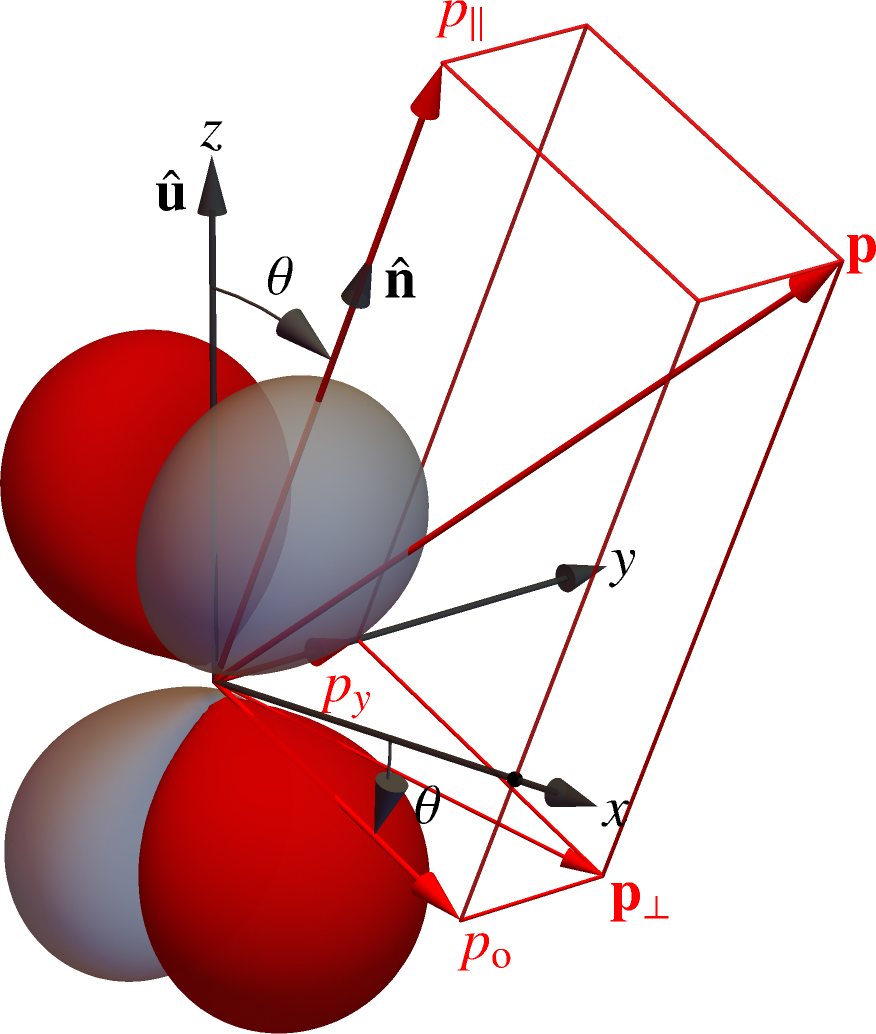
\includegraphics[scale=1]{2-ARM-theory/Figures/figure2F.png}
  \caption[Geometrical relationships between the molecular and the laser reference frames]{
  Geometrical relationships between the molecular and the laser (lab) frame. The $x$, $y$ and $z$ axis are on the molecular frame, with the internuclear axis $\uu$ along the $z$ axis. The laser polarization $\un$ is in the $x,z$ plane, with the momentum component $\pp$ along it; the transverse momentum vector $\vbpo$ has a component $\po$ in the molecular-laser ($x,z$) plane, and a shared component $p_y$ orthogonal to it.
  }
  \label{f2-molecular-frame}
\end{figure}



To tie this expression down a bit further, we introduce some additional notation to link together the molecular frame of reference with the laser, as shown in Figure~\ref{f2-molecular-frame}. We take $\un\cdot\uu=\cos(\theta)$ to give the angle $\theta$ between the internuclear axis and the laser polarization, and $\uu\cdot\vbpo=-\po\sin(\theta)$ as defining the transverse momentum component in the molecular-laser plane. With this notation, the leading-order shape factor reads
\begin{align}
\sft(\vbq)
& \approx
(-i)^n
\frac{e^{ \kappa a }}{\kappa a}
\frac{ v_x^{n_x}v_y^{\smash[b]{n_y}} v_z^{n_z}}{\kappa^{n_x+n_y+n_z}}
\cos\left(
b \left(
   \frac{\po}{\kappa}\sin(\theta)
   +i \left(1+\frac{\pt^2}{2\kappa^2}\right)\cos(\theta)
 \right)
\right)
%
\nonumber\\ & \quad   \times 
%
\left( 
1 
+ c\left(
  \frac{\po^2}{\kappa^2}\cos(2\theta)
  +\left(1+\frac{p_y^2}{\kappa^2}\right)\cos^2(\theta)
  -\frac{i}{2} \sqrt{1+\frac{\pt^2}{\kappa^2}}\frac{\po}{\kappa}\sin(2\theta)
\right)
\right)
.
\label{e2-leading-asymptotic-sft-molecular}
\end{align}


It is important to note, on the other hand, that the full analytical spherical Fourier transform $\sft(\vbq)$ as calculated in \eqref{e2-sft-final-analytical-result} does have some (unphysical) dependence on $a$, which is caused by the stack of approximations taken over the course of this chapter. This dependence disappears for large enough $\kappa a$, as shown in \reffig{f2-sft-asymptotics}, though in general this tends to happen for larger boundary radii than the equilibrium point between the laser and the Coulomb field. In practice, then, one needs to take the boundary radius $a$ at a point where the shape factor reproduces a shape consistent with the asymptotics, and is reasonably flat with respect to increases in this radius.


\captionsetup[figure]{position=above}

\newcommand{\figuretwoCkappa}{1}
\newcommand{\figuretwoCc}{1}
\newcommand{\figuretwoCb}{2.5}
\newcommand{\figuretwoCpo}{0}
\newcommand{\figuretwoCpy}{0}%
\begin{figure}[htb]
  \centering
  \begin{tabular}{cc}
  \subfloat[$n_x=0$, $n_z=0$]{
    \label{f2-sft-asymptotics-a}
    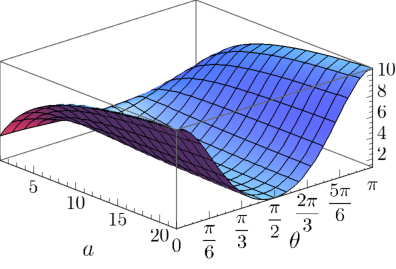
\includegraphics[scale=1]{2-ARM-theory/Figures/figure2Ca.pdf}
  }
  &
  \subfloat[$n_x=1$, $n_z=0$]{
    \label{f2-sft-asymptotics-b}
    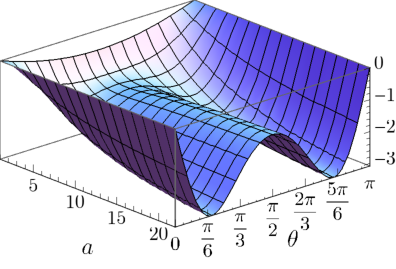
\includegraphics[scale=1]{2-ARM-theory/Figures/figure2Cb.pdf}
  }
  \\
  \subfloat[$n_x=0$, $n_z=1$]{
    \label{f2-sft-asymptotics-c}
    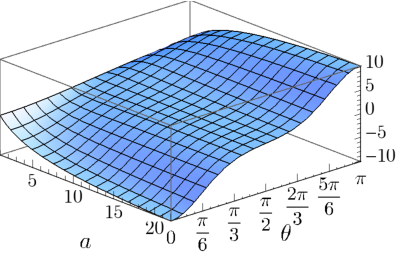
\includegraphics[scale=1]{2-ARM-theory/Figures/figure2Cc.pdf}
  }
  &
  \subfloat[$n_x=1$, $n_z=1$]{
    \label{f2-sft-asymptotics-d}
    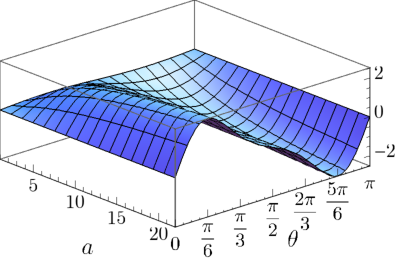
\includegraphics[scale=1]{2-ARM-theory/Figures/figure2Cd.pdf}
  }
  \end{tabular}
  \caption[Asymptotic behaviour of the spherical Fourier transform as a function of $a$]{
  Behaviour of the on-axis spherical Fourier transform, with the main asymptotic behaviour factored out as $\kappa a \:e^{-\kappa a}\:\sft(\vbq)$ and evaluated at the temporal saddle point at zero transverse momentum, as a function of the alignment angle $\theta$ and the boundary radius $a$, in the asymptotic region of the latter. 
  Here $\kappa=\figuretwoCkappa$, $c=\figuretwoCc$, $b=\figuretwoCb$, and $n_y=0$.}
  \label{f2-sft-asymptotics}
\end{figure}

%\captionsetup[figure]{position=auto}




Additionally, it is possible to go beyond the leading-order dependence of $\sft$ on $a$ and produce an asymptotic series for the limit $\kappa a \gg 1$ that produces better approximations to the shape factor (intermediate between the exact integral \eqref{e2-sft-final-analytical-result} and the leading asymptote \eqref{e2-leading-asymptotic-sft}) at moderate values of the boundary radius. Unfortunately, even to subleading order this produces rather unwieldy expressions, so they are omitted here for brevity, but they are implemented, and documented, in \citer{ARMSupport}.



More practically, the key feature of the molecular shape factor comes from its behaviour on axis: that is, for momenta very close to the laser polarization, at $\vbpo=0$, since it is harder for electrons to tunnel into nonzero transverse velocities. Thus, it is the on-axis shape factor $\left.\sft(\vbq) \right|_{\vbpo=0}$ that determines most of the effect of the electronic orbital in question and the molecule's orientation with respect to the laser field, along with its first-order dependence on $\vbpo$ at that point; we show both quantities in \reffig{f2-sft-on-axis}. 

Specifically, it is important to note that the main dependence, through $\left.\sft(\vbq) \right|_{\vbpo=0}$, will vanish when the alignment angle $\theta$ is such that the laser polarization lies along a node of the electronic orbital under consideration. In these conditions, ionization can proceed via direct ionization from other orbitals, but it can also do so via the correlation-driven mechanism which is derived below and which, as we will explore in chapter~\ref{chap:multi-channel}, relies crucially on the transverse momentum derivatives of the shape factor.





\captionsetup[figure]{position=top}
\newcommand{\figuretwoDkappa}{1.2}
\newcommand{\figuretwoDb}{2.5}
\newcommand{\figuretwoDc}{0.3}
\newcommand{\figuretwoDaone}{10}
\newcommand{\figuretwoDatwo}{50}%
\begin{figure}[htb]
  \centering
  \begin{tabular}{cc}
  \subfloat[$n_x=0$, $n_z=0$ ($-\ \Sigma_g$)]{
    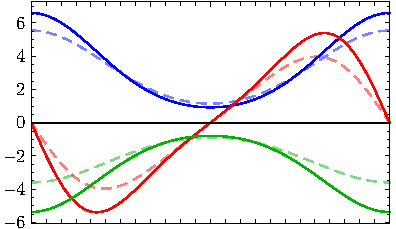
\includegraphics[scale=1]{2-ARM-theory/Figures/figure2Da.pdf}  
  }
  &
  \subfloat[$n_x=0$, $n_z=1$ ($\B\ \Sigma_u$)]{
    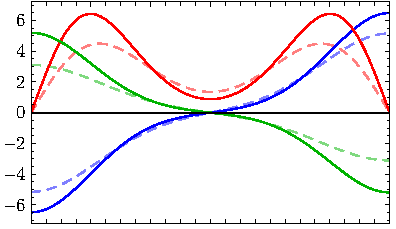
\includegraphics[scale=1]{2-ARM-theory/Figures/figure2Db.pdf}  
  }
  \\
  \subfloat[$n_x=1$, $n_z=0$ ($\A\ \Pi_u$)]{
    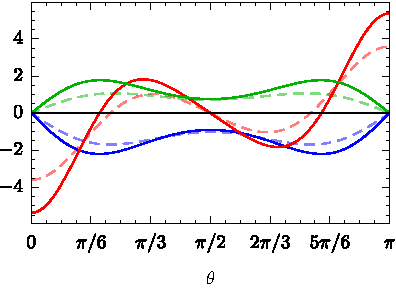
\includegraphics[scale=1]{2-ARM-theory/Figures/figure2Dc.pdf}  
  }
  &
  \subfloat[$n_x=1$, $n_z=1$ ($\X\ \Pi_g$)]{
    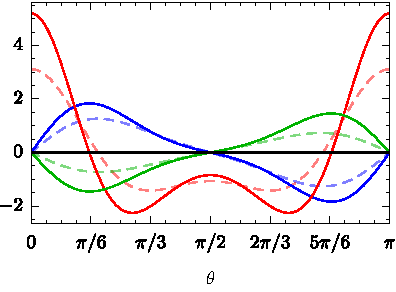
\includegraphics[scale=1]{2-ARM-theory/Figures/figure2Dd.pdf}  
  }
  \end{tabular}
  \caption[On-axis spherical Fourier transform, and its derivatives, as a function of molecular alignment angle]{Behaviour of the on-axis spherical Fourier transform $\left. \kappa a\: e^{-\kappa a}\:\sft(\vbq) \right|_{\vbpo=0}$ (blue) and its derivatives with respect to $\po$ (red) and $p_y$ (green), taken in the asymptotic region at $a=\figuretwoDatwo$. The regime of intermediate $a$, shown dashed at $a=\figuretwoDaone$, captures most of the qualitative behaviour but it is not quantitatively accurate.
  Here $\kappa=\figuretwoDkappa$, $c=\figuretwoDc$ and $b=\figuretwoDb$, corresponding to a reasonable model for the CO$_2$ molecule, and the different geometries are labelled by the orbital symmetry they produce and the corresponding states of the CO$_2$ molecule. We take $n_y=0$ for $\sft$, $\partial_\po\sft$, and the symmetry assignments, and $n_y=1$ for $\partial_{p_y}\sft$.
  }
  \label{f2-sft-on-axis}
\end{figure}
%\captionsetup[figure]{position=auto}








\section{Correlation-driven ionization}
\label{sec:correlation-driven-ionization}
We now turn to the correlation-driven ionization mechanism, which is embodied in the first-order term of the Dyson expansion of the wavefunction in powers of the correlation potential $V_{ee}^n$. We last saw this contribution in a split of the total wavefunction of the form $\ket{\Psi(t)}=\ket*{\Psi^{(0)}(t)}+\ket*{\Psi^{(1)}(t)}$ in \eqref{e2-decomposition}, in which the correlation-driven term had the form
\begin{align}
\ket{\Psi^{(1)}(t)}
=(-i)^2\sum_n  & \int\d\vb{k}\int^t\d t''\int^{t''}\d t'U^N(t,t'')V_{ee}^n(t'') U^{N-1}(t'',t')\ket{n(t')}
\nonumber \\ & \otimes 
U_e^n(t'',t')\ket{\vb{k}_n(t')}\times\matrixel{\vb{k}_n(t')}{\hat{L}^{(-)}(a)}{n_D(t')}e^{iI_p t'},
\label{e2-abstract-correlation-state-recall}
\end{align}
which we recall from \eqref{e2-abstract-correlation-state}.

The fist thing to do here is to tackle the full entangled propagator $U^N(t,t')$, which we tried to pretend was manageable by using the Dyson expansion to reduce it to a single separable propagator $U^{N-1}(t,t') \otimes U_e^n(t,t')$ but which, through the principle of conservation of hard work, is of course still present. And similarly to the first time around, to deal with this entangling propagator we will continue to pretend that it can be reduced to the unentangled dynamics, and that
\begin{equation}
U^N(t,t') \approx U^{N-1}(t,t') \otimes U_e^n(t,t')
\end{equation}
inside the integral of \eqref{e2-abstract-correlation-state-recall}. This time, however, we are no longer pushing the nontriviality away into another corner of the room: instead, we are making the definite assertion that the entangling interaction, the correlation potential $V_{ee}^n$, contributes essentially only to first order in the Dyson series, and that further interactions are negligible.

We therefore make this key physical approximation, to get the correlation-driven contribution as
\begin{align}
\ket{\Psi^{(1)}(t)}
=(-i)^2\sum_n  & \int\d\vb{k}\int^t\d t''\int^{t''}\d t'U^{N-1}(t,t'') \otimes U_e^n(t,t'')V_{ee}^n(t'') U^{N-1}(t'',t')\ket{n(t')}
\nonumber \\ & \otimes 
U_e^n(t'',t')\ket{\vb{k}_n(t')}\times\matrixel{\vb{k}_n(t')}{\hat{L}^{(-)}(a)}{n_D(t')}e^{iI_p t'},
\label{e2-abstract-correlation-state-approximate}
\end{align}
and now we can begin simplifying this using many of the techniques we used for the direct ionization channel. Thus, analogously to our definition in \eqref{e2-ionization-yield} of the ionization yield, we have the correlation-driven yield given by
\begin{align}
a_n^{(1)}(\vb{p},& \tn)
=
\bra{\vb{p}}\otimes\bra{n(\tn)}U^{N-1}(\tn,T)\ket{\Psi^{(1)}(T)}
\nonumber \\ & =
(-i)^2\sum_m  \int\!\d\vb{k}\int^T\!\!\d t''\int^{t''}\!\!\!\!\d t'
\bra{n(\tn)}U^{N-1}(\tn,t'') \otimes \bra{\vb{p}}U_e^m(T,t'')
\times V_{ee}^m(t'') 
\nonumber \\ & \quad \quad \times
U^{N-1}(t'',t')\ket{m(t')}
\otimes 
U_e^m(t'',t')\ket{\vb{k}_m(t')}
\times\matrixel{\vb{k}_m(t')}{\hat{L}^{(-)}(a)}{m_D(t')}e^{iI_p t'}.
\label{e2-correlation-driven-yield-initial}
\end{align}

Here, similarly to the direct case in \eqref{e2-propagated-quasistatic-eigenstates}, we neglect the Stark shifting and field-induced transitions between the ionic eigenstates, so the ionic states propagate as the field-free $U^{N-1}(t'',t')\ket{n(t')}=e^{-iE_n(t''-t')}\ket{n}$, and we propagate the continuum states using \eqref{e2-channel-specific-eikonal-tdse}. This leaves us, then, with a much simpler expression:
\begin{align}
a_n^{(1)}(\vb{p},\tn)
& =
(-i)^2\sum_m  \int\!\d\vb{k}\int^T\!\!\d t''\int^{t''}\!\!\!\!\d t'
e^{+iE_n(t''-\tn)}
e^{-iE_m(t''-t')}
\nonumber \\ & \qquad \quad
\times
\bra{n} \otimes \bra{\vb{p}_n(t'')}
V_{ee}^m
\ket{m}
\otimes 
\ket{\vb{k}_m(t'')}
\times\matrixel{\vb{k}_m(t')}{\hat{L}^{(-)}(a)}{m_D}e^{iI_p t'}.
\label{e2-correlation-driven-yield-second}
\end{align}

In fact, this expression separates completely into an ionization part, with a temporal integral over $t'$ -- which we term the ionization time -- and a temporal integral over $t''$, which we term the interaction time, giving
\begin{align}
a_n^{(1)}(\vb{p},\tn)
& =
-i 
e^{-iE_n \tn}
\sum_m  \int\!\d\vb{k}   \int^T\!\!\d t''
e^{+i(E_n-E_m)t''}
\bra{n} \otimes \bra{\vb{p}_n(t'')}
V_{ee}^m
\ket{m}
\otimes 
\ket{\vb{k}_m(t'')}
\nonumber \\ & \qquad \qquad \quad  \times
(-i)\int^{t''}\!\!\d t'
e^{+iE_m t'}
\matrixel{\vb{k}_m(t')}{\hat{L}^{(-)}(a)}{m_D}e^{iI_{p,m} t'}.
\label{e2-correlation-driven-yield-separated}
\end{align}
Moreover, the internal integral over the ionization time $t'$ is exactly of the same form as the direct ionization amplitude \eqref{e2-sae-yield-beginning}, with the only difference being that the upper limit, $t''$, is now variable and potentially complex, so we can directly apply the results from the previous development. The second line of \eqref{e2-correlation-driven-yield-separated} is therefore exactly equal to $e^{+iE_mt''}a_m^{(0)}(\vbk,t'')$, and it can be replaced with the final result from \eqref{e2-ionization-yield-with-shape-factor} to give
\begin{align}
a_n^{(1)}(\vb{p},\tn)
& =
-i 
e^{-iE_n \tn}
\sum_m  \int\!\d\vb{k}   \int\!\d t''
e^{+i(E_n-E_m)t''}
\bra{n} \otimes \bra{\vb{p}_n(t'')}
V_{ee}^m
\ket{m}
\otimes 
\ket{\vb{k}_m(t'')}
\nonumber \\ & \qquad \qquad \quad  \times
e^{iI_{p,m} \ts - \frac{i}{2} \int_{\ts}^{T}\left(\vbk+\vba(\tau)\right)^2\d\tau }
e^{-i\int_\tk^{t''} U_m\left(\int_{ \ts}^\tau \vbk+\vba(\tau')\d\tau'\right) \d\tau}
R_m(\vbk)
.
\label{e2-correlation-driven-yield-with-a1-included}
\end{align}

This expression admits a simple interpretation, with the electron being ionized at the complex time $\ts$ into a superposition of channels $\ket{m}$ and intermediate momenta $\vbk$, and then subsequently interacts with the ion at time $t''$ to get to its final channel $n$ and momentum $\vbp$. As far as the continuum electron is concerned, then, the main part of the interaction is the single-electron operator
\begin{equation}
\matrixel{n}{V_{ee}^m}{m}
=
\matrixel**{n}{\left(\vphantom{\sum}V_{ee}-\bra{n}V_{ee}\ket{n}\right)}{m}.
\end{equation}
This operator must be handled in the position representation, since the electrostatic interaction is defined as such by definition \eqref{e2-V-ee-definition}. We therefore encase it inside position eigenstates to get a single function of position,
\begin{equation}
\matrixel**{\vbr'}{
\vphantom{\sum}
\matrixel{n}{V_{ee}^m}{m}
}{\vbr}
=
\bra{\vbr'}\otimes\bra{n}
{\left(\vphantom{\sum}V_{ee}-\bra{n}V_{ee}\ket{n}\right)}
\ket{\vbr}\otimes\ket{m}
\equalscolon
\delta(\vbr-\vbr')
\Vnm{\vbr},
\label{e2-Vnm-definition}
\end{equation}
which we encapsulate in the shorthand notation $\Vnm{\vbr}$.

Doing the matrix element of \eqref{e2-correlation-driven-yield-with-a1-included} in the position representation, then, leaves us with the expression
\begin{align}
a_n^{(1)}(\vb{p},\tn)
& =
-i 
e^{-iE_n \tn}
\sum_m  \int\!\d\vbk   \int\!\d\vbr  \int\!\d t''
e^{+i(E_n-E_m)t''}
\Vnm{\vbr}
\braket{\vb{p}_n(t'')}{\vbr}
\braket{\vbr}{\vb{k}_m(t'')}
\nonumber \\ & \qquad \qquad \quad  \times
e^{iI_{p,m} \ts - \frac{i}{2} \int_{\ts}^{T}\left(\vbk+\vba(\tau)\right)^2\d\tau }
e^{-i\int_\tk^{t''} U_m\left(\int_{ \ts}^\tau \vbk+\vba(\tau')\d\tau'\right) \d\tau}
R_m(\vbk)
.
\label{e2-correlation-driven-yield-position-representation}
\end{align}
Here we use the explicit form of the eikonal Volkov states, \eqref{e2-eikonal-volkov-wavefunctions}, to further pin down this ionization yield into the explicit form
\begin{align}
a_n^{(1)}(\vb{p},\tn)
& =
-i 
\sum_m 
e^{-iE_n \tn}
e^{iI_{p,m} \ts}
\int\!\d t''
e^{+i(E_n-E_m)t''}
e^{-\frac{i}{2} \int_{t''}^T\left(\vbp+\vba(\tau)\right)^2\d\tau} 
\nonumber \\ & \quad \ \  \times
\frac{1}{(2\pi)^{3}}
\int\!\d\vbk
\int\!\d\vbr \:
\Vnm{\vbr}
R_m(\vbk)
e^{i\left(\vbk-\vbp\right)\cdot\vb{r}} 
e^{-\frac{i}{2} \int_{\ts}^{t''}\left(\vb{k}+\vba(\tau)\right)^2\d\tau} 
e^{-iW_{nm}(\vbr,\vbk,t'')}
%\nonumber \\ & \qquad \qquad \quad  \times
%e^{+i\int_T^{t''} U_n(\rl(\tau;\vb{r},\vbp,t''))\d\tau}
%e^{-i\int_T^{t''} U_m(\rl(\tau;\vb{r},\vb{k},t''))\d\tau}
%e^{-i\int_\tk^{t''} U_m\left(\int_{ \ts}^\tau \vbk+\vba(\tau')\d\tau'\right) \d\tau}
,
\label{e2-correlation-driven-yield-with-eva-states}
\end{align}
where the Coulomb correction now reads
\begin{align}
W_{nm}(\vbr,\vbk,t'')
& =
-\int_{t''}^T U_m(\rl(\tau;\vb{r},\vb{k},t''))\d\tau
-\int_\tk^{t''} U_m\left(\rl(\tau;\vb{0},\vb{k},t'')\right) \d\tau
\nonumber \\ & \qquad +
\int_{t''}^T U_n(\rl(\tau;\vb{r},\vbp,t''))\d\tau
.
\label{e2-correlation-channel-coulomb-correction}
\end{align}


Finally, we address the limits for the interaction-time integration over $t''$, which originally went from $-\infty$ to the large detection time $T$. However, the $t'$ integral in \eqref{e2-correlation-driven-yield-separated} only went up to $t''$, and this means that for the direct-channel result to hold we need the integration range over $t''$ to be restricted to times after the ionization event $\ts$ to which we've collapsed the entire $t'$ integral. This means, then, that the correlation-driven yield can be written down as
\begin{align}
a_n^{(1)}(\vb{p},\tn)
& =
-i 
\sum_m 
e^{-iE_n \tn}
e^{iI_{p,m} \ts}
\int_{\ts}^T\!\d t''
e^{+i(E_n-E_m)t''}
e^{-\frac{i}{2} \int_{t''}^T\left(\vbp+\vba(\tau)\right)^2\d\tau} 
\nonumber \\ & \quad \ \  \times
\frac{1}{(2\pi)^{3}}
\int\!\d\vbk
\int\!\d\vbr \:
\Vnm{\vbr}
R_m(\vbk)
e^{i\left(\vbk-\vbp\right)\cdot\vb{r}} 
e^{-\frac{i}{2} \int_{\ts}^{t''}\left(\vb{k}+\vba(\tau)\right)^2\d\tau} 
e^{-iW_{nm}(\vbr,\vbk,t'')}
%\nonumber \\ & \qquad \qquad \quad  \times
%e^{+i\int_T^{t''} U_n(\rl(\tau;\vb{r},\vbp,t''))\d\tau}
%e^{-i\int_T^{t''} U_m(\rl(\tau;\vb{r},\vb{k},t''))\d\tau}
%e^{-i\int_\tk^{t''} U_n\left(\int_{ \ts}^\tau \vbk+\vba(\tau')\d\tau'\right) \d\tau}
.
\label{e2-correlation-driven-yield-semi-final}
\end{align}
This form for $a_n^{(1)}(\vb{p},\tn)$ is now essentially ready -- or, at least, it cannot be processed much further without more knowledge about the system in question. (Here the Coulomb correction \eqref{e2-correlation-channel-coulomb-correction} can use further simplification, but we will not discuss it further and we will make the reasonable approximation that its behaviour will be similar to the correction in the direct case.) 

There are two main parts of this expression, and they fulfil two different roles. On one side there is the spatial description, which involves the integrals over $\vbr$ and $\vbk$, which determines how the geometry of both channels influences the behaviour of the correlation-driven channel, and this will be the main focus of the following chapter.

Overarching this geometrical dependence, however, is a more fundamental dynamical statement about the behaviour of this correlation-driven tunnelling, coming from the temporal integral over $t''$ and its various factors. This integral is not trivial, because in shifting the $t'$ integral to its complex saddle point $\ts$, we have also brought the starting point of the interaction-time integral over $t''$ to a complex time. Since here, as before, $t''$ appears in exponential factors of the form $e^{iEt''}$, the imaginary part of $t''$ plays a crucial~role.

At heart, the temporal dependence in \eqref{e2-correlation-driven-yield-semi-final} contains a conflict between two colliding factors that try to pull the main contributions to the integral to different regions of $t''$, and the resolution of this conflict is a compromise that makes much of the interaction happen inside the tunnelling barrier.

On one side of this conflict is the exponential factor $e^{+i(E_n-E_m)t''}$, which is a phase for real $t''$ but can provide large amplitude changes for the regions where it is complex. In general, this factor will tend to aid ionization into excited states ionic by letting the electron ionize from the highest-lying occupied orbital, which is easier to tunnel from, and then change channels once they've gone through much of the tunnelling barrier. In this case, the initial channel $m$ is the ground ionic state, and the final channel $n$ has a higher energy, so~that
\begin{equation}
\Delta I_{p,nm}=E_n-E_m
\end{equation}
is a positive quantity. In this regime, the amplitude of the exponential factor is given by
\begin{equation}
\left|e^{+i(E_n-E_m)t''}\right|
=
e^{-\Delta I_{p,nm}\Im(t'')},
\end{equation}
where in general $\Im(t'')$ will be between 0 and $\Im(\ts)>0$. This exponential dependence will tend to select interaction times with smaller imaginary parts, relatively far away from the ionization time $\ts$, and therefore as far into the barrier as possible.


On the other side of this conflict is the spatial dependence, more specifically through the decay of the interaction potential $\Vnm{\vbr}$ at larger distances. As we shall see in chapter~\ref{chap:multi-channel}, a saddle-point argument on the geometrical integrals over $\vbk$ and $\vbr$, driven by the exponential factors $\exp\left(i\left( \vbk- \vbp\right) \cdot\vb{r}-\frac{i}{2} \int_{\ts}^{t''} \left(\vb{k} + \vba(\tau) \right)^2\d\tau\right)$ of \eqref{e2-correlation-driven-yield-semi-final}, indicates that the contributions to spatial integral are mostly concentrated in a region around the laser-driven trajectory $\rl(t'') = \int_{\ts}^{t''} \vbp+\vba(\tau)\d\tau$, and this will tend to go away from the origin (and rather quickly so) as $t''$ goes from the ionization time $\ts$ towards its real part. Evaluated at this position, $\Vnm{\rl(t'')}$ will decrease in the same direction that the exponential factor is increasing. 

Taken together, both factors will make most of the interaction come from complex interaction times at which the electron is still in the mid-barrier regime, which makes the study of the interaction all the more interesting. In the following chapter we turn, therefore, to the study of the geometrical effects of this interaction, in the hopes of finding signatures that will help us show that these mid-barrier interactions are in fact occurring.



































\chapter{Multi-channel geometrical effects in tunnel ionization}
\label{chap:multi-channel}
This chapter examines the mechanism of correlation-assisted tunnelling ionization, as expressed in the correlation-driven term examined in section~\ref{sec:correlation-driven-ionization}. Here we examine the correlation-assisted contribution in terms of its geometrical features, looking for qualitative traces that can help establish, beyond pure ionization rates, the role of the correlation-assisted mechanism in tunnel ionization. We find that the direct and correlation-driven terms can have different geometrical structures, which could then be used as a way to demonstrate the presence of correlation effects in strong-field ionization. 

Some of the material in this chapter has appeared previously in reference
\begin{enumerate}
\item[{\hypersetup{citecolor=black}\citealp{Pisanty_momentum_transfers_2014}}.]
\textsc{E.~Pisanty and M.~Ivanov}.
\newblock Momentum transfers in correlation-assisted
  tunneling.
\newblock \href{http://dx.doi.org/10.1103/PhysRevA.89.043416}{
          \emph{Phys. Rev. A} \textbf{89} no.~4, p.~043\,416 (2014)}.
\newblock \href{http://arxiv.org/abs/1309.4765}{{arXiv}:1309.4765}.
\end{enumerate}
\noindent
and in the author's MRes report,
\begin{enumerate}
\item[{\hypersetup{citecolor=black}\citealp{MResReport}}.]
\textsc{E.~Pisanty}.
\newblock \emph{Under-the-barrier electron-ion interaction during tunnel
  ionization}. 
  \href{http://www3.imperial.ac.uk/controlledquantumdynamics/people/students/cohortthree/emiliopisantyalatorre }{
\newblock {MRes} report, Imperial College London (2012)}.
\newblock \href{http://arxiv.org/abs/1307.7329}{arXiv:1307.7329}.
\end{enumerate}
\noindent
This chapter mostly follows the lines of \citer{Pisanty_momentum_transfers_2014}.



\section{Electron correlation in strong-field ionization}
Throughout much of its history, and for most of its applications, strong-field physics can essentially be understood as a single-electron game, mostly because the post-ionization part of the dynamics, with the electron at the mercy of the radiation field, is at heart a single-electron phenomenon. 

However, this is at odds with the rest of atomic physics, which breaks down completely if electron correlation and exchange are not included as core parts of the theory. Within photoionization alone, for example, multi-electron effects appear in a multitude of phenomena, which include autoionizing states~\cite{fano_resonances_1961}, giant resonances~\cite{amusia_giant-resonances_2000}, shake-off~\cite{schneider_knockout-shakeoff_2002}, shake-up~\cite{matveev_shakeup_1982}, Auger and frustrated Auger decay~\cite{cooper_auger-decay_2013}, interatomic Coulomb decay~\cite{averbukh_ICD_2004}, and ultrafast correlation-driven hole migration~\cite{cederbaum_ultrafast-charge-migration_1999, kuleff_hole-migration_2005} among many others. These correlation-driven mechanisms often leave clear traces that can be used to identify them, but the distinction between different mechanisms can also be blurry, as in the case of separating the contributions of shake-up and post-ionization interaction~\cite{hino_perturbation-theory-diagrams-gauge_1993}.


Strong-field ionization, however, mostly works as a single-electron theory, as attested by the wide success of the Strong-Field Approximation in its many forms, the overwhelming majority of which are single-electron theories, or include the effect of the ionic electrons at the self-consistent-field level~\cite{pfeiffer_self-consistent-effects_2012}. The inclusion of multielectron effects beyond this level was triggered by the realization that the molecular ions produced by strong-field ionization are often electronically excited~\cite{zon_tunnelling-excitation_2000, litviniuk_shakeup_2005}, and that these excitations affect all subsequent processes~\cite{smirnova_multielectron-hhg_2009, mairesse_high-harmonic-spectroscopy_2010, torres_molecular-structure-and-dynamics-hhg_2010, haessler_attosecond-imaging_2010, lin_rescattering-self-imaging_2010}. Recent experiments~\cite{boguslavskiy_multielectron-ionization_2012, wen_n2o4-excited-ionization_2008} and \textit{ab initio} simulations~\cite{spanner_one-electron_2009,farrell_strong-field-excited-ionization_2011} confirm that, for molecules in strong fields, electronic excitations during the ionization process are the rule rather than an exception.

Two main mechanisms are responsible for creating an ion in an excited state after optical tunnelling: the laser may remove an electron from a low-lying orbital, leaving the ionic core excited~\cite{zon_tunnelling-excitation_2000, smirnova_multielectron-hhg_2009, mairesse_high-harmonic-spectroscopy_2010, torres_molecular-structure-and-dynamics-hhg_2010, haessler_attosecond-imaging_2010, lin_rescattering-self-imaging_2010, zon_many-electron_1999, zon_many-body_2010, kornev_neon-excited-ionization_2004, kornev_kinetics_2003, kornev_many-body-effects_2003, guehr_hhg-multiple-orbitals_2008}, shown schematically in \reffig{f3-direct-vs-correlated-direct}, or the electron may depart from the highest occupied molecular orbital (HOMO), and subsequently excite the core through a Coulomb interaction. This can happen inside the tunnelling barrier~\cite{walters_correlation-during-tunnelling_2010}, shown in \reffig{f3-direct-vs-correlated-midbarrier}, or after the tunnelling step~\cite{zon_tunnelling-excitation_2000, litviniuk_shakeup_2005}, as shown in \reffig{f3-direct-vs-correlated-postionization}.


\newlength{\figurethreeblwidth}
\setlength{\figurethreeblwidth}{0.3\textwidth}
\begin{figure}[htbp]
  \centering
  \subfloat[\label{f3-direct-vs-correlated-direct}]{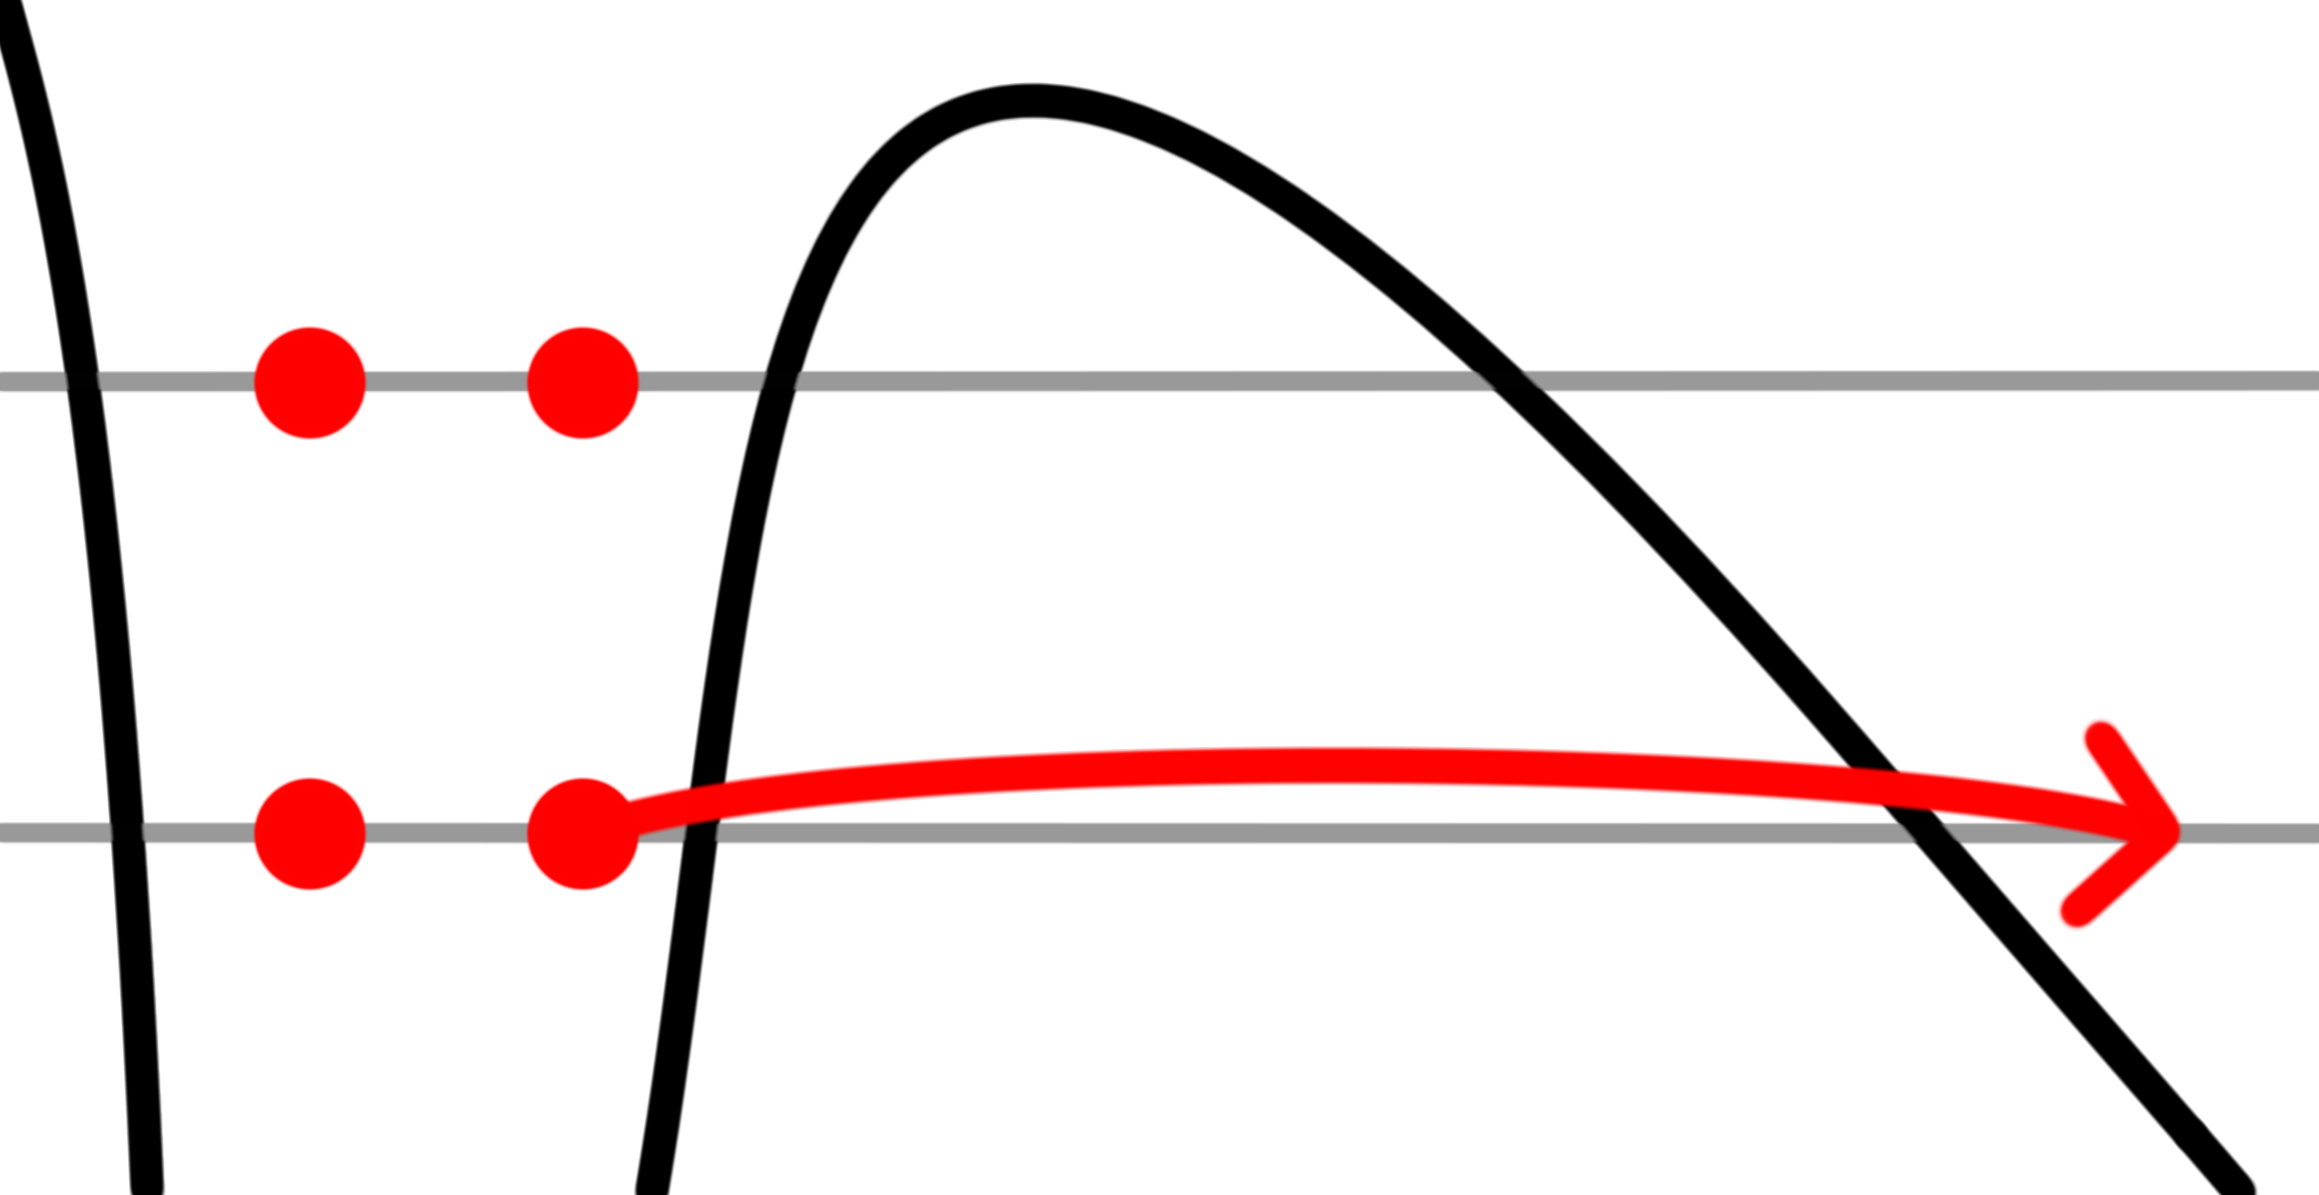
\includegraphics[width=\figurethreeblwidth]{3-Multi-channel/Figures/figure3Ba.png}}
  $\ $
  \subfloat[\label{f3-direct-vs-correlated-midbarrier}]{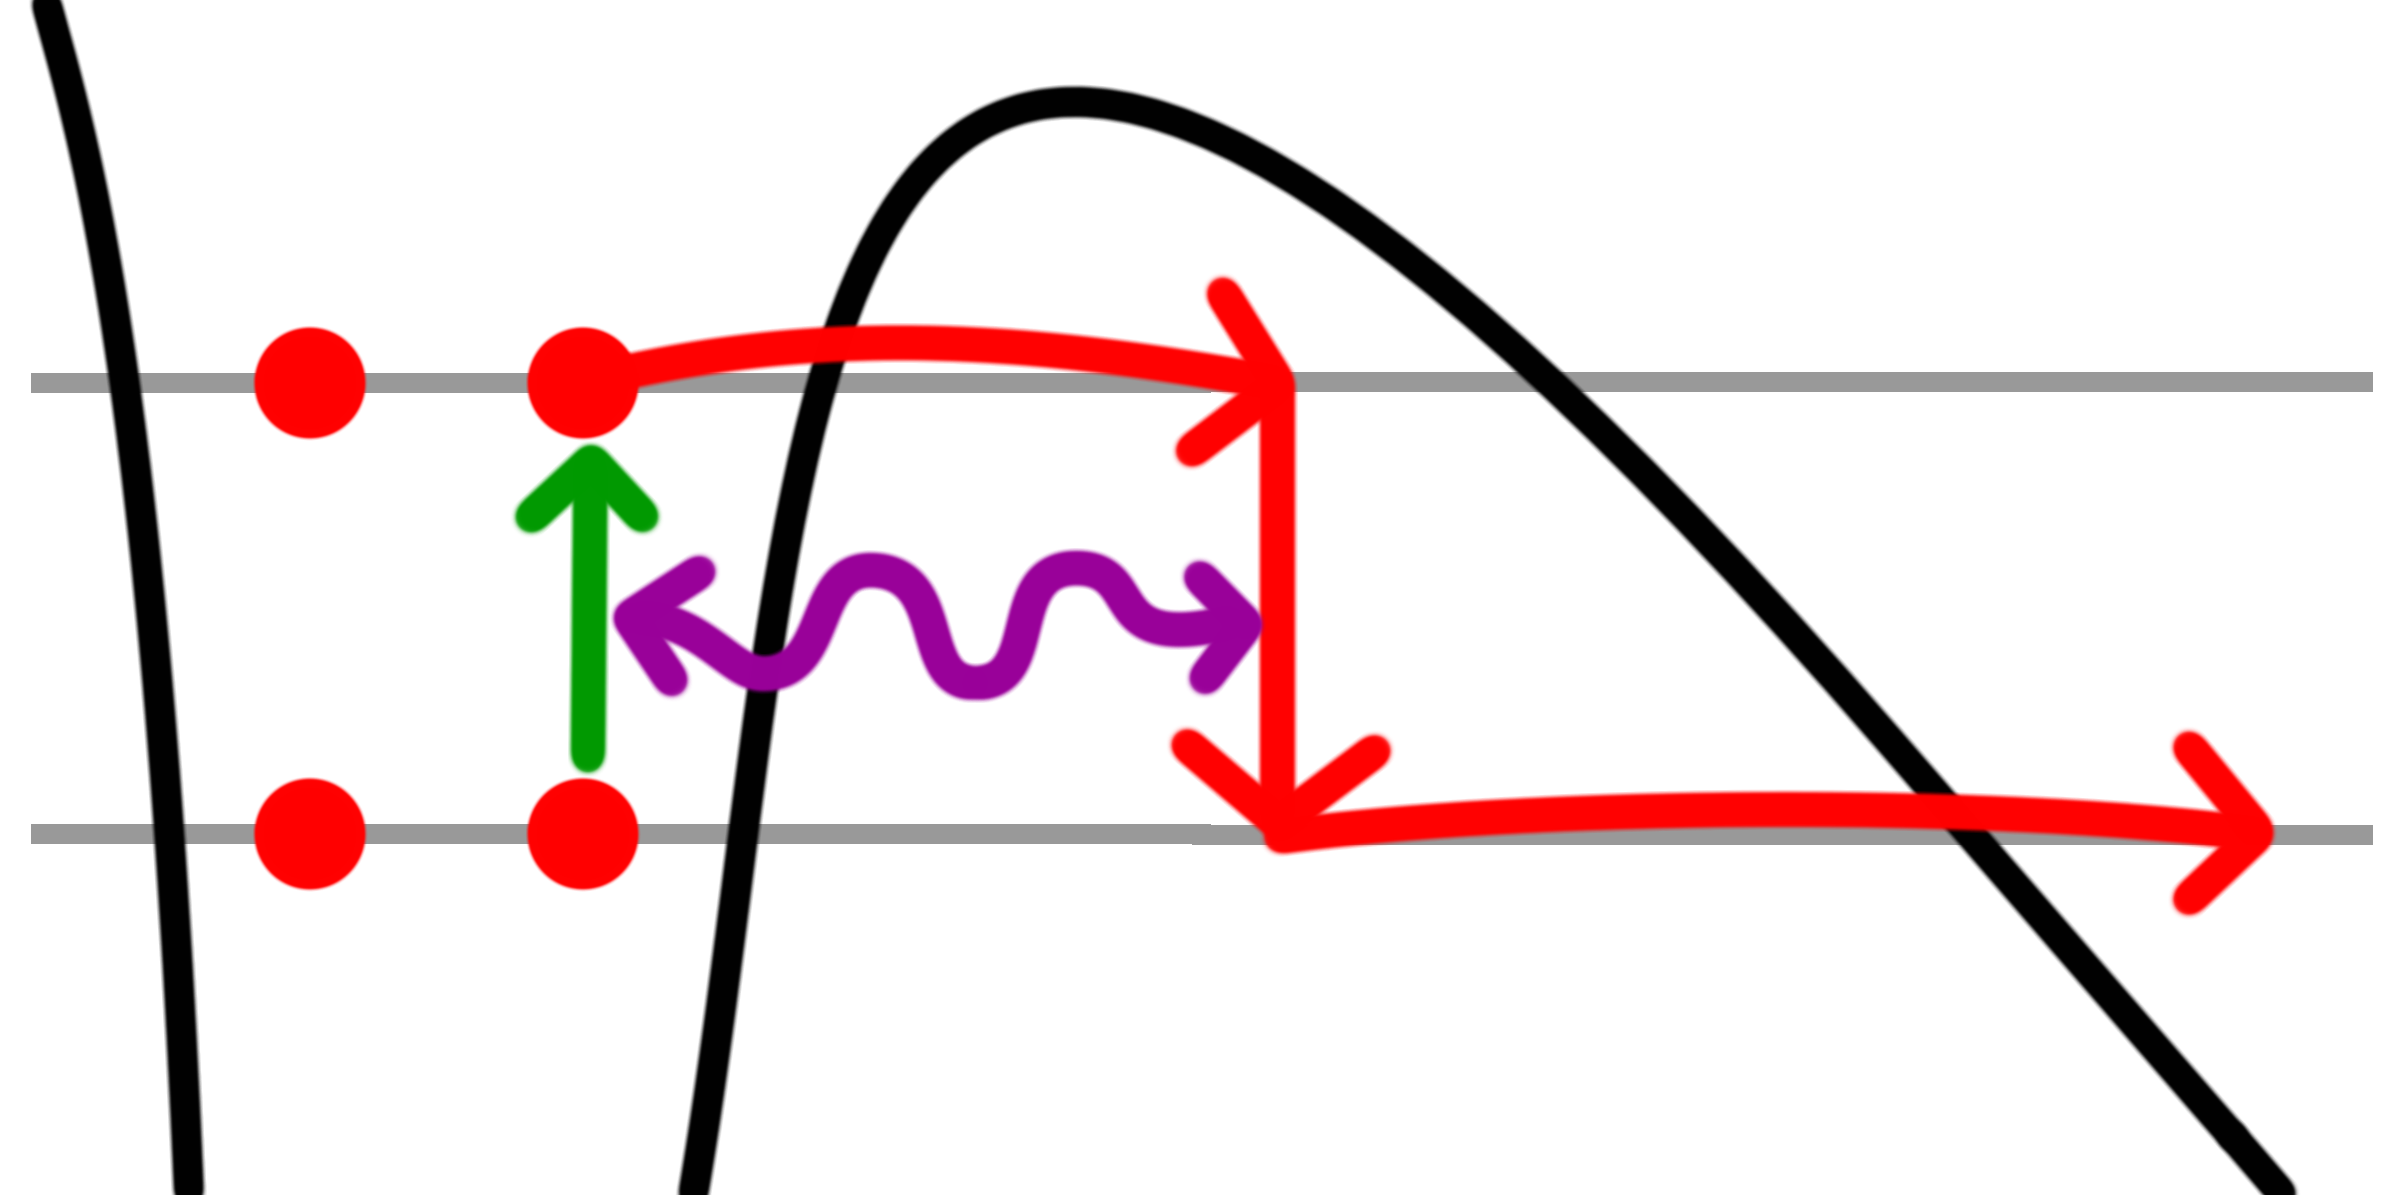
\includegraphics[width=\figurethreeblwidth]{3-Multi-channel/Figures/figure3Bb.png}}
  $\ $
  \subfloat[\label{f3-direct-vs-correlated-postionization}]{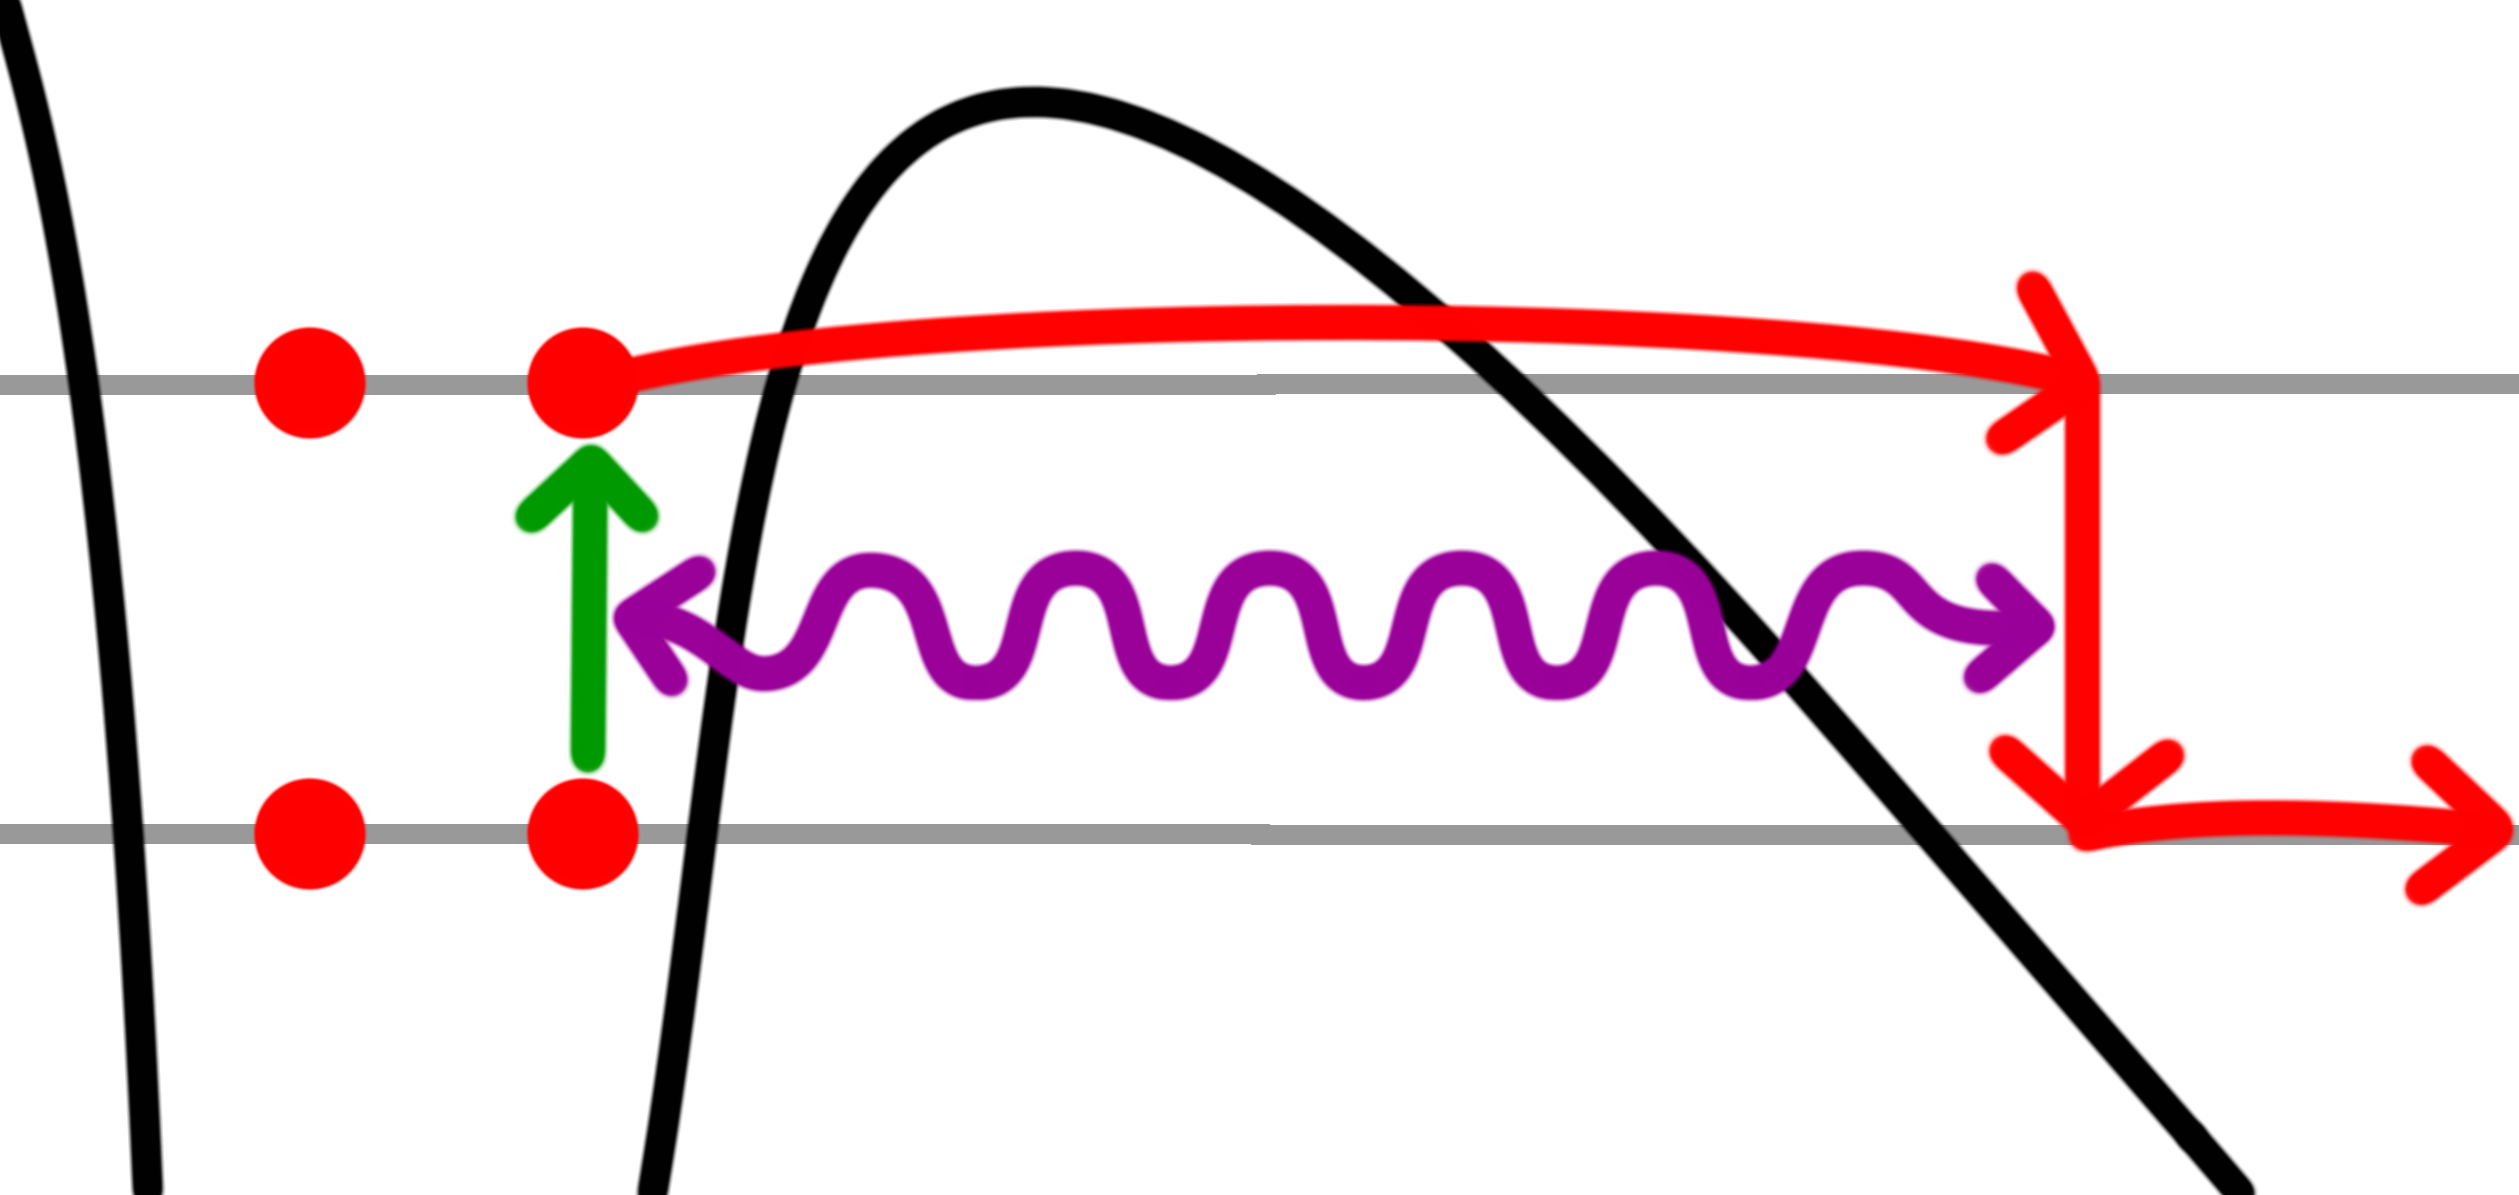
\includegraphics[width=\figurethreeblwidth]{3-Multi-channel/Figures/figure3Bc.png}}
  \caption[Three processes that leave the ion excited: direct ionization from a sub-HOMO orbital, or interaction-driven transitions before and after the tunnel exit]{Three possible ionization processes which leave the core excited: the ionized electron may depart from a sub-HOMO orbital \protect\subref{f3-direct-vs-correlated-direct}, or it may depart from HOMO and subsequently interact with the core, either inside the tunnelling barrier~\protect\subref{f3-direct-vs-correlated-midbarrier} or after the ionization step~\protect\subref{f3-direct-vs-correlated-postionization}.
  }
\label{f3-direct-vs-correlated}
\end{figure}



Analyzing strong-field ionization in a way that permits the description of electronic excitations in the ion that is left behind (and, indeed, that allows the photoelectron to return and interact with this excited ion), and to describe it in an analytical form that can help us grasp the physical mechanisms at play, is far from an easy task. Fortunately, though, our ARM theory of photoionization is perfectly capable of handling this, and indeed it was initially developed with this in mind~\cite{ ARM_initial_multielectron}. However, the original ARM implementations only considered the total ionization rates, and these do not readily yield direct, qualitative traces of the multielectron interactions that help shape the tunnelling process.

This chapter looks for such traces in the angular distribution of the photoelectron; we show that the correlation-assisted tunnelling, as shown in Figs.~\ref{f3-direct-vs-correlated-midbarrier} and \subref{f3-direct-vs-correlated-postionization}, produces wavepackets with nontrivial spatial structure as compared with the direct tunnelling of \reffig{f3-direct-vs-correlated-direct}. The correlation-driven structures, then, should interfere with the direct channel to provide clear traces, detectable in angle-resolved photoelectron spectra, that multielectron dynamics are important \textit{during} the tunnelling step.


The motivation for focusing on the transverse momentum distribution is simple. If the laser field directly removes an electron from some orbital, then the outgoing wavepacket  will carry the imprints of the spatial structure of the orbital it came from~\cite{meckel_LIED_2008}. On the other hand, if the electron switches channels by inducing transitions in the ion, then the spatial structure of the outgoing wavepacket will be due to the original orbital and the nature of the ionic transition. The resulting distribution can then be different to that of the direct removal, and it should therefore be possible to use it to distinguish the two contributions.

Additionally, the electron angular distribution is an important observable in its own right~\cite{meckel_LIED_2008, pavicic_angular-dependence-measurement_2007, zhou_angular-dependence-theory_2005, zhao_molecular-orbital-theory_2011}, both for the information it yields directly and for its strong effect on subsequent recollision dynamics, including electron-ion diffraction and holography~\cite{spanner_reading-diffraction-images_2004, yurchenko_laser-induced-rescattering_2004, blaga_imaging_2012, huismans_holography-2011}. Moreover, the observable coherence of the hole left in the ion during multi-channel ionization is directly conditioned by the overlap of the corresponding continuum electron wavepackets, since the excited ion is likely to be entangled with the ion~\cite{ruberti_thesis_2004}. It is therefore desirable to have analytical approximations for the photoelectron wavepackets, which then permit one to gauge when a small overlap between the photoelectron states implies a low available coherence for any subsequent pump-probe experiments on the state of~the~ion.


We will therefore analyse in detail the angular distributions of direct ionization from orbitals below the highest occupied molecular orbital (HOMO) and of the correlation-assisted contribution. The essentials of these distributions are determined by the symmetries of the orbitals and transitions involved, which will then allow us to look for qualitative differences in addition to quantitative predictions. We will find that, in certain geometries, the correlation-driven yield does indeed differ significantly from the shape of the direct ionization wavepacket.


We will focus, as in the previous chapter, on the channel-resolved photoelectron momentum yield $a_n(\vbp,)$ as our primary physical observable. At face value, this means that the ideal experiments will be angle- and energy-resolved photoelectron spectra, observed in coincidence with ionic state detection on aligned molecules. Such photoelectron-photoion are now becoming standard for ionic states that lead to well-defined fragments~\cite{boguslavskiy_multielectron-ionization_2012, reaction_microscope}. Alternative experiments could include recollision-based imaging experiments such as two-dimensional high-harmonic spectroscopy~\cite{shafir_resolving-tunnel-exit-times_2012} and laser-induced electron holography~\cite{spanner_reading-diffraction-images_2004, huismans_holography-2011} and diffraction~\cite{ spanner_reading-diffraction-images_2004, yurchenko_laser-induced-rescattering_2004, blaga_imaging_2012, lin_rescattering-self-imaging_2010}, which are all intrinsically sensitive to the ionic state. Moreover, the photoelectron spectrum for the direct electrons can now be measured with high~accuracy~\cite{arissian_precision-momentum-spectra_2010}.


Specifically, we will consider the tunnel ionization of CO$_2$, with the laser polarization pointing along the internuclear axis, as shown in \reffig{f3-CO2-X-to-B-coupling}. The leading perpendicular transition is from the ground-state channel of CO${}_2^+$, $\X\,\Pi_\mathrm{g}$, to its second excited channel,~$\B\,\Sigma_\mathrm{u}$. These correspond to the removal of an electron from HOMO and from HOMO$-2$, respectively, which are depicted in Figs.~\ref{f3-CO2-X-to-B-coupling-b} and~\subref{f3-CO2-X-to-B-coupling-c}.

\begin{figure}[htbp]
  \centering
  \subfloat{\label{f3-CO2-X-to-B-coupling-a}}
  \subfloat{\label{f3-CO2-X-to-B-coupling-b}}
  \subfloat{\label{f3-CO2-X-to-B-coupling-c}}
  \subfloat{\label{f3-CO2-X-to-B-coupling-d}}
  \subfloat{\label{f3-CO2-X-to-B-coupling-e}}
  \subfloat{\label{f3-CO2-X-to-B-coupling-f}}
  \subfloat{\label{f3-CO2-X-to-B-coupling-g}}
  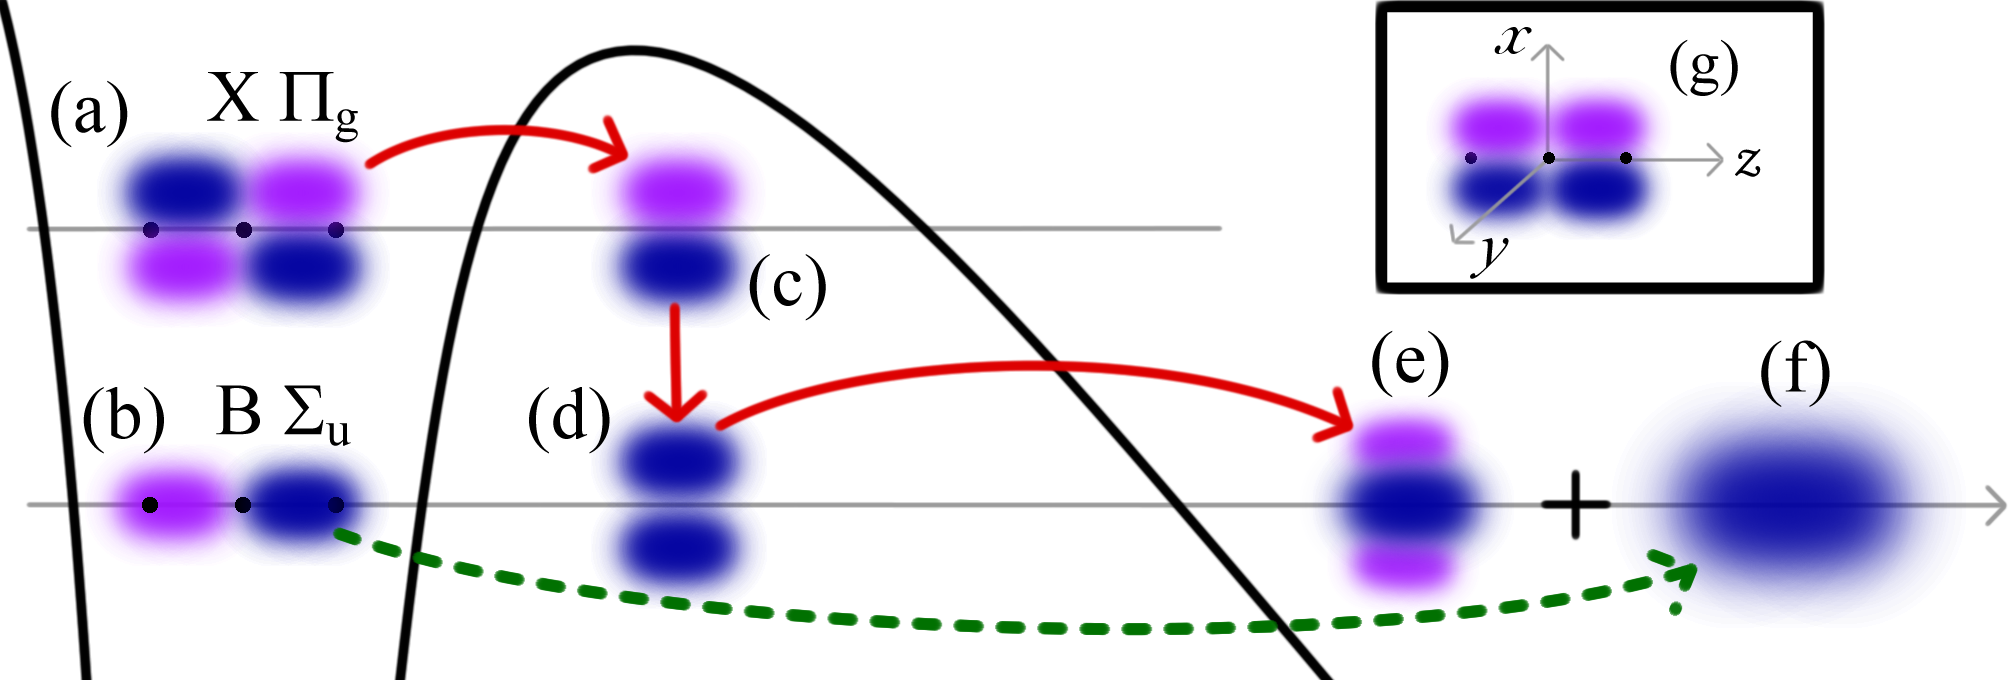
\includegraphics[width=0.75\textwidth]{3-Multi-channel/Figures/figure3C.png}
  \caption[Scheme for the correlation-assisted tunnelling of aligned CO$_2$, with the direct $\B$ channel competing with cross-channel contributions that start in the $\X$ channel.]{
  Correlation-assisted ionization of CO$_2$. An electron can ionize from HOMO~\protect\subref{f3-CO2-X-to-B-coupling-a} and change to an excited channel~\protect\subref{f3-CO2-X-to-B-coupling-b} in a mid-barrier transition~\protect\subref{f3-CO2-X-to-B-coupling-c}. This subjects it~\protect\subref{f3-CO2-X-to-B-coupling-c} to the dipole potential of the transition charge~\protect\subref{f3-CO2-X-to-B-coupling-g}, which changes the relative phase of the two lobes~\protect\subref{f3-CO2-X-to-B-coupling-d}. This double-slit wavefunction then diffracts to multiple lobes~\protect\subref{f3-CO2-X-to-B-coupling-e}. This contrasts to direct ionization on the excited $\B$ channel, which has a single~lobe~\protect\subref{f3-CO2-X-to-B-coupling-f}.
  }
\label{f3-CO2-X-to-B-coupling}
\end{figure}

Here HOMO has a nodal plane along the laser polarization (as does the HOMO$-1$ \mbox{orbital}, $\A\,\Pi_\mathrm{g}$), with two lobes of opposite phase, which means that the outgoing wavepacket inherits this structure and it is also highly suppressed, making $\B\,\Sigma_\mathrm{g}$ a substantial contributor to the ionization, despite its much higher ionization potential~\cite{meckel_LIED_2008, smirnova_multielectron-hhg_2009, mairesse_high-harmonic-spectroscopy_2010}. The position-space node is similarly reflected by a nodal plane at the origin in the momentum-space representation of the electron coming from the $\X$ orbital, embodied in the $R(\vbp)$ shape factor of the previous chapter.

At the moment of the correlation interaction $t''$, which we will integrate over as per Eq.~\eqref{e2-correlation-driven-yield-semi-final}, this wavepacket is impulsively subjected to the correlation potential $\Vnm{\vbr}$, which in this example corresponds to the electrostatic field of the transition charge. This is of the essential form $\braket{\B}{\vbr} \! \braket{\vbr}{\X}$, as depicted in \reffig{f3-CO2-X-to-B-coupling-g}, and since the transition charge is dipolar the potential will essentially be of the form $d_{\B\X}x/r^3$, in the reference frame of \reffig{f3-CO2-X-to-B-coupling-g}, with a node along the same direction as our $\X$-ionized wavepacket.%
\footnote{%
It is important to note, on the other hand, that there is an exactly equivalent channel along the $y$ axis, coming from the $\X\,\Pi_{\mathrm{g},y}$ orbital, which will restore the system's axial symmetry to our result.
}
In momentum space, our linear $\propto x$ potential is therefore proportional to the momentum operator $\frac{\partial}{\partial k_x\!\!\!{}}\,$, and it therefore transforms our two-lobed wavefunction to the three-lobed wavepacket shown in \reffig{f3-CO2-X-to-B-coupling-e}.


The physical picture is most clearly cast in terms of angular momentum. The $\X$ channel is a $\Pi$ state, which means that the outgoing electron and the hole in the core both have angular momenta $L=\pm 1$ about the laser polarization, in opposite directions. The $\B$ channel, on the other hand, is a $\Sigma$ state with zero angular momentum in the core. Inducing an $\X\rightarrow\B$ transition thus requires the outgoing electron to `wind down' the core, returning its angular momentum through the reaction force. This exchange of transverse momentum creates the central lobe.


The lateral lobes in the final momentum distribution are interference effects coming from the interaction region. In position space, the initial tunnelling wavepacket is Gaussian in the transverse direction~\cite{ivanov_anatomy_2005} with a node of the form $\psi\propto x e^{-\frac{1}{2\tau}x^2}$. The impulsive application of the dipole potential transforms it to the form $\psi'\propto x^2 e^{-\frac{1}{2\tau}x^2}$, as depicted in \reffig{f3-CO2-X-to-B-coupling-d}; the final momentum distribution is the Fourier transform of this wavefunction. The situation is then essentially interference from a double slit, formed by the two same-sign lobes of this wavefunction, with three of the fringes visible.










\section{The geometric saddle-point argument}

Having painted an intuitive picture of the process, we now move on to a more formal analysis of the resulting angular distributions. We have built, in chapter~\ref{chap:R-matrix}, most of the machinery we need, in the form of expressions \eqref{e2-ionization-yield-with-shape-factor} for the direct yield and \eqref{e2-correlation-driven-yield-semi-final} for the correlation-assisted contribution, which together~read
\begin{subequations}
\begin{align}
a_n^{(0)}(\vb{p},\tn)
& =
e^{-iE_n\tn}
e^{iI_{p,n} \ts + \frac{i}{2} \int_T^{\ts}\left(\vbp+\vba(\tau)\right)^2\d\tau }
e^{-i\int_\tk^T U_n\left(\int_{ \ts}^\tau \vb{v}(\tau')\d\tau'\right) \d\tau}
R_n(\vbp)
,
\label{e3-direct-yield-recap}
\\
a_n^{(1)}(\vb{p},\tn)
& =
-i 
\sum_m 
e^{-iE_n \tn}
e^{iI_{p,m} \ts}
\int_{\ts}^T\!\d t''
e^{+i(E_n-E_m)t''}
e^{-\frac{i}{2} \int_{t''}^T\left(\vbp+\vba(\tau)\right)^2\d\tau} 
\nonumber \\ & \quad \ \  \times
\frac{1}{(2\pi)^{3}}
\int\!\d\vbk
\int\!\d\vbr \:
\Vnm{\vbr}
R_m(\vbk)
e^{i\left(\vbk-\vbp\right)\cdot\vb{r}} 
e^{-\frac{i}{2} \int_{\ts}^{t''}\left(\vb{k}+\vba(\tau)\right)^2\d\tau} 
e^{-iW_{nm}(\vbr,\vbk,t'')}
%\nonumber \\ & \qquad \qquad \quad  \times
%e^{+i\int_T^{t''} U_n(\rl(\tau;\vb{r},\vbp,t''))\d\tau}
%e^{-i\int_T^{t''} U_m(\rl(\tau;\vb{r},\vb{k},t''))\d\tau}
%e^{-i\int_\tk^{t''} U_n\left(\int_{ \ts}^\tau \vbk+\vba(\tau')\d\tau'\right) \d\tau}
.
\label{e3-correlation-driven-yield-recap}
\end{align}
As noted above, one of the main factors that determine these amplitudes is the exponential term in the ionization time, of the form $e^{iI_{p,m} \ts}$, where the imaginary part of the ionization saddle-point time $\ts$ gives the amplitude an exponential dependence on the ionization potential $I_{p,m}$ to the given ionic state. Because of this strong dependence, these contributions will generally be limited to one or a few ionic states, and we therefore break the sum down into its different constituents
\begin{align}
a_{nm}^{(1)}(\vb{p},\tn)
& =
-i
e^{-iE_n \tn}
e^{iI_{p,m} \ts}
\int_{\ts}^T\!\d t''
e^{+i(E_n-E_m)t''}
e^{-\frac{i}{2} \int_{t''}^T\left(\vbp+\vba(\tau)\right)^2\d\tau} 
\nonumber \\ & \quad \quad  \times
\frac{1}{(2\pi)^{3}}
\int\!\d\vbk
\int\!\d\vbr \:
\Vnm{\vbr}
R_m(\vbk)
e^{i\left(\vbk-\vbp\right)\cdot\vb{r}} 
e^{-\frac{i}{2} \int_{\ts}^{t''}\left(\vb{k}+\vba(\tau)\right)^2\d\tau} 
e^{-iW_{nm}(\vbr,\vbk,t'')}
\label{e3-correlation-driven-yield-broken-down}
\end{align}
\end{subequations}
in the understanding that only their full sum, $a_n^{(1)}(\vb{p},\tn) = \sum_m a_{nm}^{(1)}(\vb{p},\tn)$ is of interest. Moreover, since in this chapter we are interested in the geometrical aspects of this amplitude, to which the Coulomb correction $e^{-iW_{nm}(\vbr,\vbk,t'')}$ contributes weakly, we will neglect it for the multi-channel analysis, assuming that it behaves mostly like the single-electron correction which we will examine in chapters \ref{chap:quantum-orbits} and \ref{chap:LES-NZES}.

As we mentioned in the previous chapter, to get a good sense of how the correlation-assisted amplitude \eqref{e3-correlation-driven-yield-broken-down} behaves, it is generally necessary to have explicit values for the interaction potential $\Vnm{\vbr}$ and the initial shape factor $R_m(\vbk)$, since these are crucial ingredients of the geometric integrals over $\vbr$ and $\vbk$. However, there is still more that we can say about the other two factors of the integrand, the exponential terms
\begin{equation}
\exp\left(\vphantom{\int} i\left(\vbk-\vbp\right)\cdot\vb{r} \right)
\exp\left( -\frac{i}{2} \int_{\ts}^{t''}\left(\vb{k}+\vba(\tau)\right)^2\d\tau \right)
,
\label{e3-exponential-factors}
\end{equation}
which also carry a strong dependence on both integration variables.

Moreover, this dependence is rather simple: although it includes an explicit integral over $\tau$, and a variable dependence on $t''$ which will later be integrated over, the exponent in this case is still simply a quadratic function of $\vbk$, which is in general relatively easy to handle. If this quadratic dependence on $\vbk$ (and, as we shall show, later on also on $\vbr$) is sharp enough, we can hope that it will be comparable to the dependence of $R_m(\vbk)$ and $\Vnm{\vbr}$ or faster, and that a saddle-point argument can apply. In any case, it is worthwhile to study this aspect of the structure of the integrand.


This is relatively easy to do, and it amounts to expanding the square in \eqref{e3-exponential-factors}, isolating the integral to powers of $\vba(\tau)$, and completing the square on $\vbk$, which yields
\begin{align}
i\left(\vbk-\vbp\right)\cdot\vb{r}
-\frac{i}{2} \int_{\ts}^{t''}\left(\vb{k}+\vba(\tau)\right)^2\d\tau
& =
-\frac i2 (t''-\ts) (\vbk-\vbk_s(\vbr))^2
-\frac i2 \mathcal{A}^2(t'')
\nonumber \\ & \qquad
+\frac{i/2}{t''-\ts} \left[
  \vbr^2 - 2\vbr \cdot \int_{\ts}^{t''} (\vbp+\vba(\tau))\d\tau  +\bm{\mathcal{A}}(t'')^2
  \right]
\label{e3-completing-squares-k}
\end{align}
in terms of the encapsulated integrals $\bm{\mathcal{A}}(t'')=\int_{\ts}^{t''}\vba(\tau)\d\tau$ and $\mathcal{A}^2(t'')=\int_{\ts}^{t''}\vba(\tau)^2\d\tau$, and the central momentum
\begin{equation}
\vbk_s(\vbr) = \frac{1}{t''-\ts} \left(  \vbr-\int_{\ts}^{t''}\vba(\tau)\d\tau  \right)
.
\label{e3-saddle-point-k}
\end{equation}
Here, however, completing the square with respect to the linear term in $\vbr \cdot \vbk$ now yields a quadratic term in $\vbr$ in the exponent, which also demands to be treated similarly. Thus, completing the square with respect to the central position
\begin{equation}
\vbr_s(\vbp) = \int_{\ts}^{t''} (\vbp+\vba(\tau))\d\tau
\label{e3-saddle-point-r-initial}
\end{equation}
we get
\begin{align}
i\left(\vbk-\vbp\right)\cdot\vb{r}
-\frac{i}{2} \int_{\ts}^{t''}\left(\vb{k}+\vba(\tau)\right)^2\d\tau
& =
-\frac i2 (t''-\ts) (\vbk-\vbk_s(\vbr))^2
+\frac{i/2}{t''-\ts} (\vbr-\vbr_s(\vbp))^2
\nonumber \\ & \qquad
-\frac i2 \int_{\ts}^{t''} (\vbp+\vba(\tau))^2 \d\tau
.
\label{e3-completing-squares-r}
\end{align}


This means, then, that the geometrical integration in \eqref{e3-correlation-driven-yield-broken-down} can be broken down into a sequence of integrals against gaussian-like kernels, as
\begin{align}
a_{nm}^{(1)}(\vb{p},\tn)
& =
-i
e^{-iE_n \tn}
e^{iI_{p,m} \ts}
\int_{\ts}^T\!\d t''
e^{+i(E_n-E_m)t''}
e^{-\frac{i}{2} \int_{t''}^T\left(\vbp+\vba(\tau)\right)^2\d\tau} 
e^{-\frac i2 \int_{\ts}^{t''} (\vbp+\vba(\tau))^2 \d\tau}
\nonumber \\ & \quad \quad  \times
\frac{1}{(2\pi)^{3}}
\int\!\d\vbr \:
e^{\frac{i/2}{t''-\ts} (\vbr-\vbr_s(\vbp))^2}
\Vnm{\vbr}
\int\!\d\vbk
e^{-\frac i2 (t''-\ts) (\vbk-\vbk_s(\vbr))^2}
R_m(\vbk)
\label{e3-correlation-driven-yield-with-completed-squares}
\end{align}
where, moreover, the $\vbp$-dependent phases come together into a single $t''$-independent integral identical to the factor in \eqref{e3-direct-yield-recap}, giving
\begin{align}
a_{nm}^{(1)}(\vb{p},\tn)
& =
-i
e^{-iE_n \tn}
e^{iI_{p,m} \ts+\frac{i}{2} \int_T^{\ts}\left(\vbp+\vba(\tau)\right)^2\d\tau} 
\int_{\ts}^T\!\d t''
e^{+i(E_n-E_m)t''}
\nonumber \\ & \quad \times
\frac{1}{(2\pi)^{3}}
\int\!\d\vbr \:
e^{\frac{i/2}{t''-\ts} (\vbr-\vbr_s(\vbp))^2}
\Vnm{\vbr}
\int\!\d\vbk  \:
e^{-\frac i2 (t''-\ts) (\vbk-\vbk_s(\vbr))^2}
R_m(\vbk)
.
\label{e3-correlation-driven-yield-with-completed-squares-2}
\end{align}


Here is where the saddle-point argument comes in. If the molecular geometrical factors $R_m(\vbk)$ and $\Vnm{\vbr}$ are relatively slow compared to the two exponentials, which is generally the case, then we are justified in considering them as constant and doing the gaussian integrals explicitly. In that case, then, the momentum integral evaluates as
\begin{equation}
\int\!\d\vbk  \:
e^{-\frac i2 (t''-\ts) (\vbk-\vbk_s(\vbr))^2}
R_m(\vbk)
=
\left(
 \frac{2\pi}{i(t''-\ts)}
 \right)^{3/2}
R_m(\vbk_s(\vbr))
,
\label{e3-geometric-integral-after-k-spa}
\end{equation}
and this feeds into the position integral to give the remarkable simple result
\begin{align}
\frac{1}{(2\pi)^{3}}
&
\int\!\d\vbr \:
e^{\frac{i/2}{t''-\ts} (\vbr-\vbr_s(\vbp))^2}
\Vnm{\vbr}
\left(
 \frac{2\pi}{i(t''-\ts)}
 \right)^{3/2}
R_m(\vbk_s(\vbr))
%
\nonumber \\ & \qquad =
%
\frac{1}{(2\pi)^{3}}
\left(
 \frac{2\pi}{i(t''-\ts)}
 \right)^{3/2}
\left(
 \frac{2\pi}{-i/(t''-\ts)}
 \right)^{3/2}
\Vnm{\vbr_s(\vbp)}
R_m(\vbk_s(\vbr_s(\vbp)))
%
\nonumber \\[5pt] & \qquad =
%
\Vnm{\vbr_s(\vbp)}
R_m(\vbk_s(\vbr_s(\vbp)))
.
\label{e3-geometrical-saddle-point-simplified}
\end{align}


One notable aspect of this development is that the saddle-point momentum (which, regardless of the validity of the geometrical saddle-point approximation, is where the two gaussian factors are concentrated) simplifies rather drastically, and it simplifies to
\begin{align}
\vbk_s(\vbr_s(\vbp)) 
& = 
\frac{1}{t''-\ts} \left(  \vbr_s(\vbp)-\int_{\ts}^{t''}\vba(\tau)\d\tau \right)
\nonumber \\ & = 
\frac{1}{t''-\ts} \left(  \int_{\ts}^{t''} (\vbp+\vba(\tau))\d\tau - \int_{\ts}^{t''}\vba(\tau)\d\tau  \right)
\nonumber \\ & = 
\vbp
,
\end{align}
that is, to the final measured momentum. More physically, this states that, within the approximations we have used, the Coulomb correlation interaction via $\Vnm{\vbr}$ between the photoelectron and the ionic core does not change the photoelectron's momentum or its kinetic energy, regardless of whether it is still under the tunnelling barrier or already outside it, but it does change the final energetic state of the ion.

(This is, of course, an approximation as far as the energy conservation law is concerned, and it is valid when $\Delta I_p\ll I_p$. Then, the modification of the outgoing trajectory is small, and the paradox is somewhat reduced. This approximation is well justified, since if $\Delta I_p$ is large then the highest-lying molecular orbital will completely dominate the ionization.)

To make this somewhat more explicit, under the geometric saddle-point approximation the correlation-driven yield reduces to the form
\begin{align}
a_{nm}^{(1)}(\vb{p},\tn)
& =
-i
e^{-iE_n \tn}
e^{iI_{p,m} \ts+\frac{i}{2} \int_T^{\ts}\left(\vbp+\vba(\tau)\right)^2\d\tau} 
R_m(\vbp)
\int_{\ts}^T\!
e^{+i(E_n-E_m)t''}
\Vnm{\rl(t'')}
\d t''
,
\label{e3-correlation-driven-yield-after-geometric-SPA}
\end{align}
which splits into a prefactor exactly equal to the direct yield \eqref{e3-direct-yield-recap} (aside from Coulomb factors, which we're neglecting in this chapter) and a temporal integral over the interaction, where we have re-labelled the position saddle point as
\begin{equation}
\rl(t) = \int_{\ts}^{t} [\vbp+\vba(\tau)]\d\tau,
\label{e3-laser-driven-trajectory}
\end{equation}
the laser-driven trajectory that starts at the origin at complex time $\ts$ and has asymptotic momentum $\vbp$. In this form, \eqref{e3-correlation-driven-yield-after-geometric-SPA} now requires explicit integration over the interaction time $t''$ of the correlation interaction potential $\Vnm{\rl(t'')}$, so in general this will have to be done numerically once a specific potential and momentum are fixed.



%More specifically, though, the imprint of the interaction on the shape of the resulting orbital is relatively weak, with the direct-tunnelling shape factor $R_m(\vbp)$ retained unchanged and only a multiplicative change via $\Vnm{ \int_{\ts}^{t''} \vbp+\vba(\tau) \, \d\tau}$ superimposed. While this 





\section{A solvable model}
In general, the saddle-point analysis just presented works fairly well, but it is concerning that the shape factor of the direct-tunnelling process, $R_m(\vbp)$, is retained intact without any change in the central momentum $\vbk_s=\vbp$, in a process which should deliver some form of momentum kick to the outgoing photoelectron when it interacts with the ionic core on its way out. 

There is, then, some tension between the physical expectation of a more specific change in the photoelectron's momentum and the mathematical expectation that, for reasonable orbital shape factors $R_m(\vbk)$ and correlation interaction potentials $\Vnm{\vbr}$, the saddle-point approximation should work well. This tension motivated, in previous work reported in the author's MRes report~\cite{MResReport}, an explicit calculation using reasonable multipolar models for both the shape factor and the interaction potential. If one compares those results with the ones from the saddle-point argument, a painful fact appears: the saddle-point approximation can fail, and rather loudly so, in this situation.

The explicit calculation of \citer{MResReport} will not be repeated here, as it is rather technical and space-intensive. Instead, this section will develop a simple toy model -- a thoroughly boiled down version of the full calculation -- for which the geometric integrals of \eqref{e3-correlation-driven-yield-broken-down} can be integrated explicitly to a result that disagrees with the saddle-point result. Moreover, this result completely encapsulates the reasons for this disagreement. As such, this toy model allows us to decide in what situations the geometrical saddle-point approximation is valid, and it points to how to fix it when it breaks. 

In terms of actual calculations for real molecules, the correlation potentials integrated over in \eqref{e3-correlation-driven-yield-after-geometric-SPA} and its modifications must be taken from quantum chemical calculations, and we will examine in chapter \ref{chap:complex-space-potentials} what happens when we require those potentials at the complex positions demanded by the laser-driven trajectory \eqref{e3-laser-driven-trajectory}, which does impose nontrivial restrictions. Nevertheless, in general it is not necessary to resort to the model potentials of \citer{MResReport} for calculations, and the simplified toy model we develop here offers an easier insight into why the geometrical saddle-point calculations need to be modified.

In short, the failure of the geometrical saddle-point approximation for \eqref{e3-correlation-driven-yield-broken-down} occurs when it predicts a zero or near-zero result, through a zero of $R_m(\vbk)$, $\Vnm{\vbr}$ or more usually both. In those conditions, the saddle-point approximation -- in reality, the leading term of an asymptotic series -- becomes comparable with, or smaller than, the sub-leading term of that series, so both terms need to be included. Doing this then returns the approximation to excellent agreement.



To appropriately model these zeroes, we refer explicitly for our toy model to the transition we chose, the $\X\to\B$ transition in CO$_2$ aligned along the laser polarization, as shown earlier in \reffig{f3-CO2-X-to-B-coupling}. In this configuration, the initial $\X\:\Pi_\mathrm{g}$ orbital has a node along the laser polarization, so its shape factor is of the form
\begin{equation}
R_m(\vbk)=C_m(k_z)k_x = \frac{C_{0,m}}{\sqrt{iS_V''(\ts)}}k_x.
\end{equation}
The correlation interaction potential, on the other hand, as defined in \eqref{e2-Vnm-definition}, is caused by the overlap density between the $\X$ and $\B$ orbitals, shown in \reffig{f3-CO2-X-to-B-coupling-g}, which as we argued earlier must also have a node along the laser polarization. The simplest model, then is a dipolar interaction, so we take
\begin{equation}
\Vnm{\vbr}=\frac{d_{mn}x}{(z^2+\sigma^2)^{3/2}}.
\end{equation}
This is a standard dipolar interaction, going down as $1/r^3$, where we've replaced $r$ by the longitudinal coordinate $z$ for simplicity and to reflect the generally small angle of ionization, and we've added a softening by $\sigma$ to account for the finite size of the molecular dipole charge. This potential does not account for all of the true potential's spatial variation, but it captures the essence that interests us in this chapter.


We can now put in these explicit factors into the geometrical factors of the correlation-assisted yield \eqref{e3-correlation-driven-yield-broken-down}, and this gives us
\begin{align}
I_\mathrm{geom}
& =
\frac{1}{(2\pi)^{3}}
\int\!\d\vbk
\int\!\d\vbr \:
\Vnm{\vbr}
R_m(\vbk)
e^{i\left(\vbk-\vbp\right)\cdot\vb{r}} 
e^{-\frac{i}{2} \int_{\ts}^{t''}\left(\vb{k}+\vba(\tau)\right)^2\d\tau} 
\nonumber \\ & =
\frac{1}{(2\pi)^{3}}
\int\!\d\vbk
\int\!\d\vbr \:
\frac{d_{mn}x}{(z^2+\sigma^2)^{3/2}}
C_m(k_z)k_x
e^{i\left(\vbk-\vbp\right)\cdot\vb{r}} 
e^{-\frac{i}{2} \int_{\ts}^{t''}\left(\vb{k}+\vba(\tau)\right)^2\d\tau} 
\nonumber \\ & =
I_x I_y I_z
,
\end{align}
a well-defined geometrical integral that can now be tackled directly, and which moreover splits cleanly into component parts.

From these, the $y$ component is essentially trivial, since at
\begin{equation}
I_y
=
\frac{1}{2\pi}
\int \! \d k_y \! \int \! \d y \:
e^{i(k_y-p_y)y}
e^{-\frac{i}{2} (t''-\ts)k_y^2}
\end{equation}
it is a pair of simple gaussian integrals, so the saddle-point result is exact, giving $I_y=1$ as per \eqref{e3-geometrical-saddle-point-simplified}. Similarly, the longitudinal $z$ component can generally be well approximated by the saddle-point integration, as long as $C_m(k_z)$ is slow enough, in which case that integral~reads
\begin{align}
I_z
& =
\frac{1}{2\pi}
\int \! \d k_z \! \int \! \d z \:
\frac{C_m(k_z)}{(z^2+\sigma^2)^{3/2}}
e^{i(k_x-p_x)x}
e^{-\frac{i}{2} \int_{\ts}^{t''}\left(k_z+A_z(\tau)\right)^2\d\tau}
\nonumber \\ & =
\frac{C_m(p_z)}{(z(t'')^2+\sigma^2)^{3/2}}
e^{-\frac{i}{2} \int_{\ts}^{t''}\left(p_z+A_z(\tau)\right)^2\d\tau}
,
\end{align}
exactly analogously to the previous case.


The problem, as expected, is in the $x$ part of the geometrical integral, since this is the direction where we have put both of the relevant nodes, in $x$ and in $k_x$:
\begin{equation}
I_x
=
\frac{1}{2\pi}
\int \! \d k_x \! \int \! \d x \:
d_{mn}x k_x
e^{i(k_x-p_x)x}
e^{-\frac{i}{2} (t''-\ts)k_x^2}
.
\end{equation}
This is, again, pretty close to a gaussian integral, and it can be done exactly. In fact, for the first step of integration, over $k_x$, the saddle-point method is again exact, since the prefactor splits as
\begin{equation}
k_x=(k_x-k_x^{(s)})+k_x^{(s)},
\end{equation}
where the first term is odd about $k_x^{(s)}$ and gives a zero integral with respect to the even gaussian kernel, leaving only the constant term at the saddle point. Splitting the exponent as in \eqref{e3-completing-squares-r}, then, gets us
\begin{align}
I_x
& =
\frac{d_{mn}}{2\pi}
e^{-\frac{i}{2} (t''-\ts)p_x^2}
\int 
x \,
e^{\frac{i/2}{t''-\ts}\left(x-x^{(s)}\right)^2}
\int 
k_x\,
e^{-\frac{i}{2} (t''-\ts)\left(k_x-k_x^{(s)}\right)^2} 
\d k_x \,
\d x
\nonumber \\ & =
\frac{d_{mn}}{2\pi}
\left(
 \frac{2\pi}{i(t''-\ts)}
 \right)^{1/2}
e^{-\frac{i}{2} (t''-\ts)p_x^2}
\int 
x \,
k_x^{(s)} \,
e^{\frac{i/2}{t''-\ts}\left(x-x^{(s)}\right)^2}
\d x
,
\label{e3-Ix-integral-after-k-integration}
\end{align}
where the saddle point as per \eqref{e3-saddle-point-k} is given by $k_x^{(s)}= x/(t''-\ts)$, so the integral is given~by
\begin{align}
I_x
& =
\frac{d_{mn}}{2\pi}
\left(
 \frac{2\pi}{i(t''-\ts)}
 \right)^{1/2}
\frac{
 e^{-\frac{i}{2} (t''-\ts)p_x^2}
 }{t''-\ts}
\int 
x^2 \,
e^{\frac{i/2}{t''-\ts}\left(x-x^{(s)}\right)^2}
\d x
\label{e3-Ix-integral-with-x2-node}
\end{align}
with a saddle point at $x^{(s)}=(t''-\ts)p_x$.

Here, finally, lies the root of the failure of the saddle-point approximation for the geometrical integrals, at the failure of the approximation for integrals of the form
\begin{equation}
\int 
x^2 \,
e^{\frac{i/2}{t''-\ts}\left(x-x^{(s)}\right)^2}
\d x
.
\end{equation}
At low transverse momenta, $p_x\approx 0$, the saddle point $x^{(s)}=(t''-\ts)p_x$ is very close to the quadratic zero of the prefactor at $x=0$, which means that the saddle-point approximation when taken naively will yield a zero value for the integral. However, even at $p_x=x^{(s)}=0$, the area under the curve $x^2e^{-x^2}$, shown in \reffig{f3-gaussian-with-node}, is simply not zero.


\begin{figure}[htb]
  \centering
  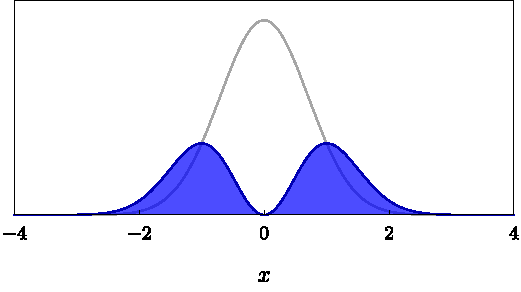
\includegraphics[scale=1]{3-Multi-channel/Figures/figure3A.pdf}
  \caption[Plots of $e^{-x^2}$ and $x^2e^{-x^2}$ as functions of $x$]{Plots of $e^{-x^2}$ and $x^2e^{-x^2}$ as functions of $x$, with the (nonzero) area under the latter shaded in blue.}
  \label{f3-gaussian-with-node}
\end{figure}



This simply means, of course, that the saddle-point approximation needs to be modified to take explicit care of this possibility. In its usual form, approximating an integral of the form $\int_A^B F(\zeta) e^{\rho \varphi(\zeta)} \d\zeta$ by the value $F(\zeta_s) e^{\rho\varphi(\zeta_s)}$ of its integral at the saddle point $\zeta_s$ comes from neglecting the spatial variation of $F(\zeta)$ near the saddle point, i.e., from replacing it with its zeroth-order Taylor expansion there. For cases like $x^2e^{-x^2}$, one simply needs to take an appropriate number of terms in the Taylor series, which -- like $\int x^2 e^{-x^2} \d x$ -- can also be integrated exactly.






\begin{mathaside}{The saddle-point approximation for saddle points near zeros of the prefactor}
\label{aside.SPAreprise}
\noindent
To make this more precise in general, consider again  an analytic function $F$ which varies slowly with respect to the analytic exponent $\varphi$, integrated as $\int_A^B F(\zeta) e^{\rho \varphi(\zeta)}\d\zeta$ over a contour that includes a single saddle point $\zeta_s$ such that $\varphi'(\zeta_s)=0$. Taking an $N$-term Taylor expansion for $F$, and the leading-order expansion for $\varphi$, at $\zeta_s$ gives an expansion of the form
\begin{equation}
\int_A^B F(\zeta) e^{\rho \varphi(\zeta)}\d\zeta
\approx
\sum_{n=0}^{2N}\frac{F^{(n)}(\zeta_s)}{n!}  e^{\rho \varphi(\zeta_s)}\int_A^B (\zeta-\zeta_s)^n  e^{\frac12 \rho \varphi ''(\zeta_s)(\zeta-\zeta_s)^2} \d\zeta
,
\end{equation}
with only the leading order term in the expansion of $\varphi$ contributing because of the exponential effect of a large $\rho$.

\vspace{\maskip}
In this expansion, all the odd powers of $\zeta-\zeta_s$ disappear, because they give an integrand of odd overall symmetry about $\zeta_s$, leaving only the even terms of the form $\zeta^{2n}e^{-\zeta^2}$ integrated over a contour which (in the asymptotic regime of~$\rho\to\infty$) is much longer than the dimensions of the gaussian envelope. Extending the contour to infinity, the integrals can then be performed exactly~\cite{BruijnAsymptotics, GerlachSPAonline}, and this gives the approximation
\begin{equation}
\int_A^B F(\zeta) e^{\rho \varphi(\zeta)}\d\zeta
\approx
\sqrt{\frac{2\pi}{\rho}} 
\frac{e^{\rho\varphi(\zeta_s)}}{\left[-\varphi''(\zeta_s)\right]^{1/2}}
\sum_{n=0}^N
\frac{(-1)^n}{n!}
\frac{
  F^{(2n)}(\zeta_s) 
  }{
  \left(2\rho\varphi''(\zeta_s)\right)^n
  }
.
\label{e3-full-SPA-statement}
\end{equation}

In general, the Taylor series should not be taken to too high a degree $N$, as this would push the relevant contributions too far from the saddle point and closer to points where the ends of the contour, or other saddles, could interfere. In a formal sense, the approximation \eqref{e3-full-SPA-statement} only works as an asymptotic series, in which more terms can only be included when the asymptotic parameter $\rho$ is large~enough. 

For our purposes, though, this expansion serves its purpose at the leading-term level, except when the prefactor is too small at the saddle point, in which case only one or two additional terms need to be included.
\end{mathaside}


Coming back to our integral, we now see that the saddle-point approximation is again exact -- if taken to the second order, which is of course the exact integration we want. Thus, we have
\begin{equation}
\int 
x^2 \,
e^{\frac{i/2}{t''-\ts}\left(x-x^{(s)}\right)^2}
\d x
=
\left(
 \frac{2\pi}{-i/(t''-\ts)}
 \right)^{1/2}
\left(
\left(x^{(s)}\right)^2 + i (t''-\ts)
\right)
,
\end{equation}
where the quadratic term in $x^{(s)}\propto p_x$ is the usual saddle-point contribution, which is dominated at low $p_x$ by the second-order term, a constant with respect to $p_x$. Putting in this integral into $I_x$, then, we have the exact expression
\begin{align}
I_x
& =
%\frac{d_{mn}}{2\pi}
%\left(
% \frac{2\pi}{i(t''-\ts)}
% \right)^{1/2}
%\frac{
% e^{-\frac{i}{2} (t''-\ts)p_x^2}
% }{t''-\ts}
%\int 
%x^2 \,
%e^{\frac{i/2}{t''-\ts}\left(x-x^{(s)}\right)^2}
%\d x
%\\ & =
i d_{mn}
e^{-\frac{i}{2} (t''-\ts)p_x^2}
\left(  1 - i(t''-\ts)p_x^2  \right)
e^{-\frac{i}{2} (t''-\ts)p_x^2}
,
\label{e3-Ix-final}
\end{align}
and this is what determines the angular profile of the correlation-driven wavefunction for this geometry.


Here there are several observations worth making. The first is that the angular distribution for this cross-channel is indeed very different to what we would have obtained using the direct saddle-point argument, as shown in \reffig{f3-angular-distribution-plots}. The angular profile for this channel now has a nontrivial structure with sign changes across the distribution, and this would not be obtained otherwise. Moreover, the angular structure of the cross channel is distinct from that of the direct channel, so their final interference -- at amplitudes and phases still to be determined -- will in general also have an interesting angular variation.


\begin{figure}[htb]
  \centering
  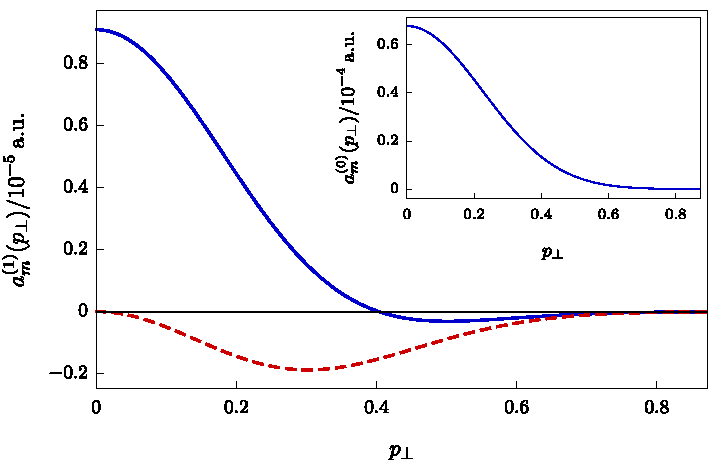
\includegraphics[scale=1]{3-Multi-channel/Figures/figure3D.pdf}
  \caption[Transverse ionization spectra for aligned CO$_2$, coming from the direct and correlation-driven channels, as well as the geometrical saddle-point approximation to the latter]{
  Momentum-resolved ionization yield for the $\X\to\B$ perpendicular dipole transition in parallel-aligned CO$_2$, with the corresponding direct amplitude in the inset. The dashed curve is the prediction from the spatial saddle-point approximation.
  The parameters used are $F=\SI{0.05}{\au}$ and $\omega=\SI{0.057}{\au}$ (so $I=\SI{9e13}{W/cm^2}$ and $\lambda=\SI{800}{nm}$), $d_{\B\X}=\SI{0.175}{\au}$, $\sigma=\SI{2.19}{\au}$, $C_{0,\X}=\SI{0.23}{\au}$, $C_{0,\B}=\SI{0.18}{\au}$, $I_{p,\X}=\SI{0.5064}{\au}$, and $I_{p,\X}=\SI{0.6644}{\au}$
  }
  \label{f3-angular-distribution-plots}
\end{figure}


Somewhat more physically, it is important to remark that the central lobe of \reffig{f3-angular-distribution-plots} is purely a wave phenomenon, caused by the Fourier transformation, via $e^{ip_xx}$, of the gaussian-with-a-hole wavefunction that results from taking the two-lobed gaussian that results from the direct tunnelling in the initial channel, of the form $k_x e^{-\Delta t k_x^2}$, and multiplying it by a transition operator proportional to $\Vnm{\vbr}\propto x$. That is, as tunnelling goes on, the wavefunction forms in position space in the form $x^2 e^{ix^2/\Delta t}$, and this looks (since $\Delta t$ is imaginary) much like the function in \reffig{f3-gaussian-with-node}. In essence, this is a double-slit wavefunction, as depicted in \reffig{f3-CO2-X-to-B-coupling}, and the momentum distribution determined by \eqref{e3-Ix-final} is precisely the far-field diffraction pattern caused by this double slit. To make this a bit more interesting, though, since the pattern forms primarily while $t''$ is still complex and the photoelectron is still inside the tunnelling barrier, the far-field angular distribution shown in \reffig{f3-angular-distribution-plots} is a diffraction pattern that originates from a matter-wave double slit that occurs inside a tunnelling~barrier, as shown in the step from \subref{f3-CO2-X-to-B-coupling-d} to \subref{f3-CO2-X-to-B-coupling-e} in \reffig{f3-CO2-X-to-B-coupling}.









\section{Modified saddle-point arguments for real molecules}
As we have seen, the saddle-point approximation can fail when compared to exact calculations for toy models of experimentally relevant geometries. Unfortunately, the route of exact calculation faces a rather steep uphill climb if it is to describe realistic molecules. One such example is the calculation in \citer{MResReport}, which models the molecule via relatively simple descriptors of the form
\begin{equation}
R_m(\vbk)=C(k_z)e^{im_1\phi_k}k_\perp^{|m_1|}
\quad \text{and} \quad
\Vnm{\vbr}=\frac{Q_{\ell m_2}}{r^{\ell+1}}Y_{\ell m_2}(\theta, \phi)
,
\end{equation}
and still only obtains a result in series form. For a realistic molecule, this is an unsatisfactory model because in the neighbourhood of the molecule the presence of ionic electrons makes the correlation interaction potential $\Vnm{\vbr}$ a solution of the Poisson (rather than the Laplace) equation. Moreover, obtaining a good model for a given molecule in terms of multipolar potentials is not particularly easy. Other analytically integrable models are also possible, but they also present significant challenges.

In general, the electronic structure of the remaining ion -- the ionic states $\{\ket{n}\}$ and the properties that emanate from them -- is a problem for quantum chemistry, and indeed the discipline has much to say on the subject of our correlation interaction potential $\Vnm{\vbr}$. While the numerical, quantum chemical evaluation of $\Vnm{\vbr}$ is still the cleanest and simplest way ot the quantity, unfortunately there are some rather fundamental difficulties and limitations to computing this quantity when it is queried at the complex trajectories that interest us, which we will explore in chapter \ref{chap:complex-space-potentials}.

In this paradigm, of course, exact analytical integration of the geometrical integrals is ruled out, since $\Vnm{\vbr}$ can only be queried numerically. This is a reasonable solution in the saddle-point approximation in which \eqref{e3-correlation-driven-yield-with-completed-squares-2} is reduced to \eqref{e3-correlation-driven-yield-after-geometric-SPA} giving
\begin{align}
a_{nm}^{(1)}(\vb{p},\tn)
& =
-i
e^{-iE_n \tn}
e^{iI_{p,m} \ts+\frac{i}{2} \int_T^{\ts}\left(\vbp+\vba(\tau)\right)^2\d\tau} 
\int_{\ts}^T\!\d t''
e^{+i(E_n-E_m)t''}
\nonumber \\ & \quad \times
\frac{1}{(2\pi)^{3}}
\int\!\d\vbr \:
e^{\frac{i/2}{t''-\ts} (\vbr-\vbr_s(\vbp))^2}
\Vnm{\vbr}
\int\!\d\vbk  \:
e^{-\frac i2 (t''-\ts) (\vbk-\vbk_s(\vbr))^2}
R_m(\vbk)
\nonumber \\ & \approx
-i
e^{-iE_n \tn}
e^{iI_{p,m} \ts+\frac{i}{2} \int_T^{\ts}\left(\vbp+\vba(\tau)\right)^2\d\tau} 
\int_{\ts}^T\!
R_m(\vbp)
\Vnm{\rl(t'')}
e^{+i(E_n-E_m)t''}
\d t''
,
\end{align}
since here $\Vnm{\vbr}$ only needs to be queried at a limited set of positions for the temporal integration. As we've seen, though, this direct saddle-point approximation is flawed, but the roots of the flaw are clear and it can be fixed by suitable modifications of the saddle-point approximation. Doing this then permits us to perform the temporal integral over $t''$ with only one (or a few) evaluations of $\Vnm{\vbr}$ per temporal integration point.


To reformulate the geometrical saddle-point method, then, we need to look for the quadratic zeros of the $\vbr$ and $\vbk$ integrand. In general, though, we can be rather more specific than that, since if only $p$ orbitals are involved, with linear nodes at most, then the emergence of zeroes is always as in \eqref{e3-Ix-integral-after-k-integration} and \eqref{e3-Ix-integral-with-x2-node}, with linear nodes in both factors combining to make a more complicated quadratic zero. In terms of our previous development, this means that we can interrupt the saddle-point method just after the $\vbk$ integration of \eqref{e3-geometric-integral-after-k-spa}, at which point the ionization yield reads

\begin{align}
a_{nm}^{(1)}(\vb{p},\tn)
& =
-i
e^{-iE_n \tn}
e^{iI_{p,m} \ts+\frac{i}{2} \int_T^{\ts}\left(\vbp+\vba(\tau)\right)^2\d\tau} 
\int_{\ts}^T\!\d t''
e^{+i(E_n-E_m)t''}
\nonumber \\ & \quad \times
\frac{1}{(2\pi)^{3}}
\left(
 \frac{2\pi}{i(t''-\ts)}
 \right)^{3/2}
\int\!\d\vbr \:
\Vnm{\vbr}
R_m(\vbk_s(\vbr))
e^{\frac{i/2}{t''-\ts} (\vbr-\vbr_s(\vbp))^2}
.
\label{e3-correlation-driven-yield-reprise-after-k-integral}
\end{align}


Here, then, we apply our extended saddle-point approximation \eqref{e3-full-SPA-statement}, going to second order in the derivatives of the prefactor. In contrast to our original development of the approximation, though, here we have multiple dimensions to handle, so taking the subleading terms should be interpreted as taking only the second derivative in each dimension and adding them up (i.e., ignoring terms of the form $\frac{\partial^2\varphi}{\partial x^2} \frac{ \partial^2 \varphi}{\partial y^2}$), which cleanly yields a rotation-invariant Laplacian of the $\vbr$-dependent prefactor.

This means, then, that our previous \eqref{e3-geometrical-saddle-point-simplified} should be reformulated to read

\begin{align}
\frac{1}{(2\pi)^{3}}
&
\left(
 \frac{2\pi}{i(t''-\ts)}
 \right)^{3/2}
\int\!\d\vbr \:
\Vnm{\vbr}
R_m(\vbk_s(\vbr))
e^{\frac{i/2}{t''-\ts} (\vbr-\vbr_s(\vbp))^2}
%
\nonumber \\ & \quad =
%
\frac{1}{(2\pi)^{3}}
\left(
 \frac{2\pi}{i(t''-\ts)}
 \right)^{3/2}
\left(
 \frac{2\pi}{-i/(t''-\ts)}
 \right)^{3/2}
\times
%
\nonumber \\ & \quad \quad \times
%
\left[
 \Vnm{\vbr_s(\vbp)}
 R_m(\vbk_s(\vbr_s(\vbp)))
 +
 \frac{i}{2} (t''-\ts)
 \nabla_{\vbr}^2
 \left(
   \vphantom{\sum}
   \Vnm{\vbr}
   R_m(\vbk_s(\vbr))
 \right)_{\vbr_s(\vbp)}
\right]
%
\nonumber \\[3pt] & \quad =
%
\Vnm{\vbr_s(\vbp)}
R_m(\vbk_s(\vbr_s(\vbp)))
 +
 \frac{i}{2} (t''-\ts)
 \nabla_{\vbr}^2
 \left(
   \vphantom{\sum}
   \Vnm{\vbr}
   R_m(\vbk_s(\vbr))
 \right)_{\vbr_s(\vbp)}
.
\label{e3-geometrical-saddle-point-reprise-r}
\end{align}
%
%
Moreover, here the second derivative that acts on the product $\Vnm{\vbr} R_m(\vbk_s(\vbr))$ really only needs to pick out the cross terms that arise from the conjunction of linear zeroes in each factor. As such, it can generally be simplified to the form
\begin{align}
\nabla_{\vbr}^2
\left(
  \vphantom{\sum}
  \Vnm{\vbr}
  R_m(\vbk_s(\vbr))
\right)
%
& \approx
%
2 \left( \nabla_{\vbr}\Vnm{\vbr} \right)
\cdot
\left( \nabla_{\vbr} R_m(\vbk_s(\vbr)) \right)
%
\nonumber \\ & =
%
\frac{2}{t''-\ts} 
\left( \nabla_{\vbr}\Vnm{\vbr} \right)
\cdot
\left( \nabla_{\vbk} R_m(\vbk_s(\vbr)) \right)
\end{align}
with the factor of $t''-\ts$ coming from the derivative of $\vbk_s(\vbr)$ with respect to $\vbr$ as per \eqref{e3-saddle-point-k}. Putting this approximation into \eqref{e3-geometrical-saddle-point-reprise-r} then gives us


\begin{align}
\frac{1}{(2\pi)^{3}}
&
\left(
 \frac{2\pi}{i(t''-\ts)}
 \right)^{3/2}
\int\!\d\vbr \:
\Vnm{\vbr}
R_m(\vbk_s(\vbr))
e^{\frac{i/2}{t''-\ts} (\vbr-\vbr_s(\vbp))^2}
%
\nonumber \\ & \quad \approx
%
\Vnm{\vbr_s(\vbp)}
R_m(\vbk_s(\vbr_s(\vbp)))
+
i
\nabla_{\vbr}\Vnm{\vbr_s(\vbp)}
\cdot
\nabla_{\vbk} R_m(\vbk_s(\vbr_s(\vbp))) 
\label{e3-geometrical-saddle-point-with-explicit-grad-dot-grad}
\end{align}
for the geometrical integrals, and 
\begin{align}
a_{nm}^{(1)}(\vb{p},\tn)
& =
-i
e^{-iE_n \tn}
e^{iI_{p,m} \ts+\frac{i}{2} \int_T^{\ts}\left(\vbp+\vba(\tau)\right)^2\d\tau} 
\int_{\ts}^T\!\d t''\:
e^{+i(E_n-E_m)t''}
\nonumber \\ & \qquad \quad \times
\left(
\vphantom{\sum}
\Vnm{\rl(t'')}
R_m(\vbp)
+
i
\nabla_{\vbr}\Vnm{\rl(t'')}
\cdot
\nabla_{\vbp} R_m(\vbp) 
\right)
.
\label{e3-correlation-driven-yield-reprise-with-full-derivatives}
\end{align}
for the final correlation-driven yield.

This expression, then, addresses the failures of the saddle-point approximation clearly exhibited by the toy model, while still retaining the simplicity and numerical ease afforded by the saddle-point method. Here we are spared the need for a full $\vbr$ integration at each time step, and instead we require only a single evaluation of $\Vnm{\vbr}$ and one of its derivatives, $\nabla_{\vbr}\Vnm{\vbr}$. Moreover, depending on the method used to calculate $\Vnm{\vbr}$, the calculation of the gradient can be relatively cheap, when done numerically, and it can even fall out essentially for free from the same quantum chemical calculations that yield the potential.


















\chapter{Molecular electrostatic potentials in complex space}
\label{chap:complex-space-potentials}



As we have seen in chapters \ref{chap:R-matrix} and \ref{chap:multi-channel}, the $R$-matrix correlation-driven yield can be written down as \eqref{e3-correlation-driven-yield-reprise-with-full-derivatives}, which is essentially of the form
\begin{align}
a_{nm}^{(1)}(\vb{p},\tn)
& =
-i
e^{-iE_n \tn}
e^{iI_{p,m} \ts+\frac{i}{2} \int_T^{\ts}\left(\vbp+\vba(\tau)\right)^2\d\tau} 
\int_{\ts}^T\!
e^{+i(E_n-E_m)t''}
\Vnm{\rl(t'')}
R_m(\vbp)
\d t''
\label{e4-correlation-driven-yield-recap}
\end{align}
if we ignore for the moment our hard-won corrections from chapter~\ref{chap:multi-channel} (which are nevertheless of an equivalent form) as well as the Coulomb corrections of chapter~\ref{chap:R-matrix}. From this expression we know essentially everything we need to get some hard numbers, except for the correlation interaction potential
\begin{equation}
\Vnm{\vbr}=\matrixel**{n}{\sum_{j=1}^{N-1} \frac{1-\delta_{nm}}{\| \vbr - \hat{\vbr}_j\|} }{m}
.
\label{e4-correlation-interaction-potential-initial}
\end{equation}
The purpose of this chapter is to examine this potential as a function of $\vbr$. 

This is in principle rather straightforward, as it is only the expectation value of a Coulomb kernel -- a bread-and-butter component of quantum chemistry -- but as we have seen before, we need to query this potential at the laser-driven trajectory
\begin{equation}
\rl(t) = \int_{\ts}^{t} \left[ \vbp+\vba(\tau) \right] \: \d\tau,
\end{equation}
and in general this is complex: the ionization time $\ts$ from \eqref{e2-ts-equation} is complex, so the integration variable $\tau$ must be complex, and this forces the analytical vector potential $\vba(\tau)=-\frac{F}{\omega}\ue_{z} \sin(\omega \tau)$ to also be complex. In chapter~\ref{chap:quantum-orbits} we will explore the structure of this complex-valued trajectory -- how complex it can be, how that interacts with the correlation interaction potential and the mean-field Coulomb potential, and to what extent the imaginary parts of $\rl(t)$ can be kept to a minimum -- but, for the moment, this chapter simply accepts that $\Vnm{\vbr}$ needs to be queried at complex-valued arguments, and studies the consequences.


We will find that for several common models of the orbitals that generate $\Vnm{\vbr}$, including models general enough to generate the state of the art numerical calculations for the orbitals, the corresponding analytical continuations for $\Vnm{\vbr}$ can agree surprisingly well (when $\vbr$ is `real~enough'), but they can also differ catastrophically (when $\vbr$ is `too~imaginary'), or even be impossible to generalize into a correct analytical continuation. 

The result is a serious constraint on the positions at which we can reliably calculate $\Vnm{\vbr}$ (and indeed even know what behaviour to expect), and a strong argument can be made that we completely lack the tools to venture further. On the other side, this limit also increases our confidence in $\Vnm{\vbr}$ in the regions where we \textit{can} calculate it, and, moreover, it gives us a clear goal to address in chapter~\ref{chap:quantum-orbits}, where we will show that it is indeed possible to steer the complex trajectory $\rl(t'')$ so that we never need to query $\Vnm{\rl(t'')}$ at the positions where the numerical methods fail and the analytical models disagree.



\section{Quantum chemical calculations of correlation interaction potentials for real positions}

For a real argument $\vbr$, the correlation interaction potential in \eqref{e4-correlation-interaction-potential-initial} is actually rather straightforward to calculate, since it is just the matrix element of a function of the $\vbr_j$ between two well-defined ionic eigenstates. As such, one can simply insert a position-space resolution of the identity,
\begin{equation}
1
=
\int\!\d\vbr_1\cdots\d\vbr_{N-1} \:
\ket{\vbr_1,\ldots,\vbr_{N-1}}\bra{\vbr_1,\ldots,\vbr_{N-1}}
,
\end{equation}
to rephrase the potential as an $(N-1)$-dimensional integral:
\begin{equation}
\Vnm{\vbr}
=
\sum_{j=1}^{N-1} 
\int\!
\frac{
  \braket{n}{\vbr_1,\ldots,\vbr_{N-1}} \!
  \braket{\vbr_1,\ldots,\vbr_{N-1}}{m}
  }{
  \| \vbr - \vbr_j\|
  }
\d\vbr_1\cdots\d\vbr_{N-1} 
.
\label{e4-correlation-interaction-potential-integral}
\end{equation}
(For convenience, we forget the factor of $\delta_{mn}$, which requires us to remember to impose $n\neq m$ on all uses of $\Vnm{\vbr}$.)

In general, for real $\vbr$, these are are well-behaved integrals. They have integrable square-root singularities at $\vbr_j=\vbr$, where the Coulomb kernel is multiplied by the transition charge density $ \braket{n}{\vbr_1,\ldots,\vbr_{N-1}} \!  \braket{\vbr_1,\ldots,\vbr_{N-1}}{m}$ (which is in principle complex-valued), and these are in generally smooth and rather well-behaved, with support confined to rather small regions around the molecule.


We can get a lot of intuition about the correlation interaction potentials of the form \eqref{e4-correlation-interaction-potential-integral} by working in the simplest Hartree-Fock regime, in which the ground state
\begin{equation}
\ket{\Psi_g} = \mathbb{A}\ket{\phi_1}\otimes \cdots\otimes \ket{\phi_N}
\end{equation}
is a minimal Hartree-Fock determinant, a single antisymmetrized product of single-particle orbitals $\ket{\phi_j}$, and the ionic eigenstates can be approximated well by simply deleting the relevant orbitals from the ground state. In this case the correlation interaction potential simplifies to a one-particle integral of the form
\begin{equation}
\Vnm{\vbr}
=
\sum_{j=1}^{N-1} 
\int\!
\frac{
  \phi_n^*(\vbr')\phi_m(\vbr')
  }{
  \| \vbr - \vbr'\|
  }
\d\vbr'
\label{e4-correlation-interaction-potential-hartree-fock}
\end{equation}
or, in terms of a transition charge $\rho_{mn}(\vbr') = \phi_n^*(\vbr') \phi_m(\vbr')$, as 
\begin{equation}
\Vnm{\vbr}
=
\int\!
\frac{
  \rho_{mn}(\vbr')
  }{
  \| \vbr - \vbr'\|
  }
\d\vbr'
.
\label{e4-correlation-interaction-potential-with-transition-charge}
\end{equation}
For rigorous calculations, one should of course use the fullest form available, but the Hartree-Fock intuition is useful in predicting the overall behaviour of $\Vnm{\vbr}$. For example, this form justifies our use of a dipole model for the $\X\to\B$ transition in $\mathrm{CO}_2$ in chapter~\ref{chap:multi-channel}.


Similarly, the full-form potential \eqref{e4-correlation-interaction-potential-integral} can also be written down in the single-particle integral form \eqref{e4-correlation-interaction-potential-with-transition-charge} by using the slightly more complicated transition charge density
\begin{align}
\rho_{mn}(\vbr')
 =
(N-1)
\int\!
\d\vbr_2 \cdots \d\vbr_{N-1} 
&   
\braket{n}{\vbr',\vbr_2,\ldots,\vbr_{N-1}} \!
%\nonumber \\ & \qquad \times
\braket{\vbr',\vbr_2,\ldots,\vbr_{N-1}}{m}
,
\label{e4-full-transition-charge-as-integral}
\end{align}
which encapsulates the $\vbr$-independent integration over all the other electrons.

Either way, the correlation interaction potential can always be written down in the form \eqref{e4-correlation-interaction-potential-with-transition-charge}, as a simple single three-dimensional integral of some transition charge $\rho_{mn}(\vbr')$ times a standard, perfectly integrable Coulomb kernel. As such, the correlation interaction potential can be thought of as the electrostatic field that would be produced by a charge density $\rho_{mn}(\vbr')$, complex-valued as it might be.



In practice, unfortunately, obtaining exact analytical expressions for $\Vnm{\vbr}$ for realistic cases is impossible, starting with the fact that there are no molecules for which we know exact analytical solutions for the electronic eigenstates. In fact, even for the simplest known molecular system, the hydrogen molecular ion H$_2^+$, with only a single electron responding to two clamped nuclei, the single-dimensional Schrödinger equation is separable but not exactly solvable. Similarly, as soon as there is more than one electron present -- starting with atomic helium -- exact analytical solutions of the Schrödinger equation simply do not exist.

The response to this over the past eight decades has been to develop numerical methods to solve the Schrödinger equation to as good a precision as one can reasonably ask for, by using some suitable discretization of the available state space and then numerically solving a finite-dimensional eigenvalue problem, and this is the core of the discipline of quantum chemistry. 

Within this discipline, the prevailing methods to discretize the state space for the electron wavefunctions involve the postulation of some finite basis of single-electron functions,
\begin{equation}
B=\left\{\chi_1,\ldots,\chi_M\right\},
\end{equation}
possibly optimized for the problem at hand in some variational way, and then working with $n$-electron wavefunctions built as linear combinations of Slater determinants of those basis functions. In general, these basis functions are mostly chosen to be so-called Slater-type orbitals of the form $e^{-r/\alpha}$, depending exponentially on the distance $r$ to some fixed point in space, or even more commonly gaussian-type orbitals of the form $e^{-r^2/\sigma^2}$, both of which can be modified by polynomial factors to give them better angular momentum properties.

In the end, though, what matters for our purposes is that the transition charge density $\rho_{mn}(\vbr')$, when calculated through quantum chemical means, will typically be completely constrained to be finite linear combinations of gaussian densities centred at some arbitrary location in the molecule, possibly multiplied by some polynomial. This then allows us to replace the arbitrary-looking $\rho_{mn}(\vbr')$ by a fixed gaussian charge density
\begin{equation}
\rhog(\vbr')=\normg \exp(-r'^2/\sigma^2)
\label{e4-gaussian-charge-density}
\end{equation}
if it is necessary to build intuition for the behaviour of the potential \eqref{e4-correlation-interaction-potential-with-transition-charge} when it is calculated via quantum chemical means, in the informal understanding that the full quantum chemical transition charge density is a linear superposition of such densities or polynomially related ones, and therefore so will the potential, which depends linearly on $\rho_{mn}(\vbr')$.


Here it is important to note that the gaussian potential \eqref{e4-gaussian-charge-density} is not quite a perfect model for a transition charge of the form \eqref{e4-full-transition-charge-as-integral}, because transition charges must always integrate to zero:
\begin{align}
\int \!
\rho_{mn}(\vbr')
\, \d\vbr'
& =
(N-1)
\int\!
\d\vbr' \,
\d\vbr_2 \cdots \d\vbr_{N-1} 
\braket{n}{\vbr',\vbr_2,\ldots,\vbr_{N-1}} \!
\braket{\vbr',\vbr_2,\ldots,\vbr_{N-1}}{m}
\nonumber \\ & =
\braket{n}{m}
= 0
.
\end{align}
In terms of simplified models, the gaussian potential \eqref{e4-gaussian-charge-density} can easily be modified to have this property, with the simplest and most physically relevant example being a $p$-type gaussian of the form $\rho_{\mathrm{g}, z} (\vbr')=z'\rhog(\vbr')$. The results in this chapter are essentially unchanged with this modification (which is most easily seen by noting that $\rho_{\mathrm{g}, z} (\vbr')$ is the derivative of $\rhog(\vbr')$ with respect to shifts in the origin), though the loss of rotational symmetry makes the analysis more awkward.

Similarly, when quantum chemists use simple gaussians as a basis to represent a transition charge, the nature of the coefficients is always such that, although each term, as in \eqref{e4-gaussian-charge-density} or multiplied by a polynomial, will have a nonzero charge, all these charges must add to zero.



\section{Quantum chemical potentials for complex positions}
\label{sec:quantum-chemical-potentials-complex}
Somewhat more practically, even for simple gaussian charge densities of the form \eqref{e4-gaussian-charge-density}, it is often cheap enough to simply perform the integral \eqref{e4-correlation-interaction-potential-with-transition-charge} for $\Vnm{\vbr}$ numerically, since it is relatively well behaved (its integrable singularity aside) and can be computed relatively quickly. For a quantum chemical transition charge density, known numerically in terms of the eigenfunctions of a finite-dimensional problem, this certainly seems to be a rather reasonable route, and for real positions it tends to work well.


What we want, of course, is to extend \eqref{e4-correlation-interaction-potential-with-transition-charge} to complex positions, but at least as a first stab it is reasonable to simply put in a complex-valued $\vbr$ and churn away at the numerical integral. In this case, then the integral is of the form
\begin{align}
\Vnm{\vphantom{\sum} \Re(\vbr)+i\Im(\vbr)}
& =
\int\!
\frac{
  \rho_{mn}(\vbr')
  \: \d\vbr'
  }{
  \sqrt{ \left( \Re(\vbr)+i\Im(\vbr) - \vbr' \right)^2 }
  }
\nonumber \\ & =
\int\!
\frac{
  \rho_{mn}(\vbr')
  \: \d\vbr'
  }{
  \sqrt{ \left( \Re(\vbr)-\vbr' \right)^2 - \Im(\vbr)^2 + 2i\Im(\vbr)\cdot (\Re(\vbr)-\vbr')}
  }
,
\label{e4-correlation-interaction-potential-with-complex-position}
\end{align}
which is not all that problematic, at least at first glance.

There is, for sure, the issue of exactly what branch to take for the square root, but unless there are strong over-riding reasons this is settled by the fact that -- absent knowledge of $\vbr$ and the support through $\rho_{mn}(\vbr')$ for the $\vbr'$ that are relevant to the integral -- the argument of the square root is in general conjugate-symmetric with respect to inversion in $\vbr'$ (i.e. inverting $\vbr'$ roughly conjugates the square root argument), and this generally requests that the square root be taken in a conjugate-symmetric way. This requires, then, that we define the square root with a branch cut on the ray $(-\infty,0]$, so
\begin{equation}
\sqrt{\zeta}=\sqrt{|\zeta|e^{i\theta}} = |\zeta|^{1/2} e^{i\theta/2}
\label{e4-square-root-definition}
\end{equation}
whenever the argument $\zeta$ is written as $\zeta=|\zeta|e^{i\theta}$ for $-\pi< \theta \leq \pi$. Throughout this work we will adhere strictly to this convention for the symbol $\sqrt{\phantom{zz}}$ unless otherwise noted.


\begin{subequations}
In addition to this, the change from real to complex $\vbr$ does change the structure of the integrand, by changing the nature of the singularity in the denominator. More concretely, having a vanishing denominator now requires a \textit{pair} of conditions,
\begin{align}
\left( \Re(\vbr)-\vbr' \right)^2 & = \Im(\vbr)^2 \quad \text{and} \\
 (\vbr'-\Re(\vbr)) \cdot \Im(\vbr) & =0,
\end{align}
and this changes the dimensionality of the singularity from a point to (in general) a non-degenerate line. This singularity is now the intersection of a plane through the $\Re(\vbr)$ orthogonal to $\Im(\vbr)$ and a sphere of radius $\|\Im(\vbr)\|$ around $\Re(\vbr)$, and this means that whenever $\Im(\vbr)\neq 0$ it is always a circle of radius $\|\Im(\vbr)\|$ centred at $\Re(\vbr)$, on a plane orthogonal to $\Im(\vbr)$.
\label{e4-circular-singularity}%
\end{subequations}%

Here the added dimension does make the singularity less noble -- there's ``more singularity'' to handle -- but it is still perfectly manageable, since locally at the singularity it looks mostly like a straight line, so it is of the form
\begin{equation}
\int_\mathrm{local}  \frac{\d x'\d y'\d z'}{\sqrt{(x'-x_0)^2+(y'-y_0)^2}}
\end{equation}
(i.e. with the $z$ dimension regularized out, but still a line singularity at $x'=x_0$, $y'=y_0$), and this is still regular when the area element in the $x',y'$ plane $\d x'\d y'=r'\d r'\d\theta'$ is taken into account. Of course, if the integration is done numerically the ring singularity must still be specifically handled to obtain correct results, but it does not represent a significant impediment to the calculation.


\captionsetup[figure]{position=top}
\begin{figure}[htb]
  \centering
  \begin{tabular}{cc}
  \subfloat[$\Re(\Vg(\vbr))$]{
    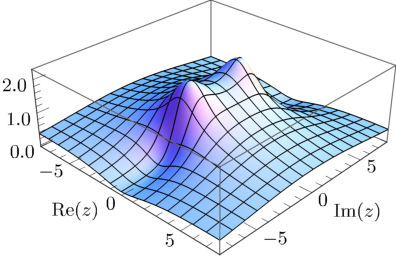
\includegraphics[scale=1]{4-Potentials/Figures/figure4Aa.pdf}
  }
  &
  \subfloat[$\Im(\Vg(\vbr))$]{
    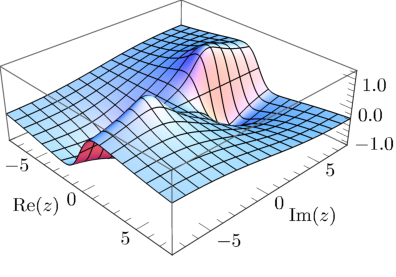
\includegraphics[scale=1]{4-Potentials/Figures/figure4Ab.pdf}
  }
  \end{tabular}
  \caption[Numerically integrated electrostatic potential $\Vg(\vbr)$ of a gaussian charge distribution as a function of complex space coordinates]{
  Electrostatic potential $\Vg(\vbr)$ of a gaussian charge distribution as a function of complex $z$ for fixed $x=3$ and $y=0$, with $\sigma=1$, calculated using direct numerical integration as in \eqref{e4-correlation-interaction-potential-numerically-gaussian}.}
  \label{f4-numerical-potential-from-gaussian}
\end{figure}
\captionsetup[figure]{position=auto}


With all this in hand, then, we can now simply plug in a complex position into \eqref{e4-correlation-interaction-potential-with-complex-position}, do the integral numerically, and see what comes out. As a starting example, to keep things simple, we can use a single gaussian charge distribution at the origin, $\rhog(\vbr)$ as in \eqref{e4-gaussian-charge-density}, so we look to calculate
\begin{align}
\Vg\left(\vphantom{\sum} \Re(\vbr)+i\Im(\vbr)\right)
& =
\int\!
\frac{
  \normg \exp(-r'^2/\sigma^2)
  \: \d\vbr'
  }{
  \sqrt{ \left( \Re(\vbr)-\vbr' \right)^2 - \Im(\vbr)^2 + 2i\Im(\vbr)\cdot (\Re(\vbr)-\vbr')}
  }
.
\label{e4-correlation-interaction-potential-numerically-gaussian}
\end{align}
This single integral can readily be integrated numerically, and we show the results in \reffig{f4-numerical-potential-from-gaussian}, fixing two components of $\vbr$ and showing the variation of $\Re(\Vg(\vbr))$ and $\Im(\Vg(\vbr))$ as a function of complex $z$ while keeping $x$ and $y$ constant. (Because of the rotational symmetry of $\rhog(\vbr)$, of course, these results are essentially representative, up to the shape parameter $\sqrt{x^2+y^2}/\sigma$.)




This procedure, then, gives us a very workable electrostatic potential: it is continuous, with no poles, branch points, or other singularities, and it is bounded at infinity. More physically, it contains two large bumps when $z=i\zeta$ is imaginary and of the same magnitude as $|x|$ because then the quadratic term $\Re(\vbr^2)=x^2-\zeta^2$ in
\begin{align}
\Vg(x,0,i\zeta)
& =
\int\!
\frac{
  \normg \exp(-r'^2/\sigma^2)
  \: \d\vbr'
  }{
  \sqrt{r'^2-2(xx'+i\zeta z')+(x^2-\zeta^2)}
  }
,
\end{align}
which effectively acts as softening, vanishes, and this leaves the Coulomb kernel at maximal amplitude. Moreover, the potential appears to be smooth and, if everything went right, it should be analytic.





Unfortunately, this combination of features turns out to be too good for our electrostatic potential, because it makes it run afoul of one of the basic principles of complex analysis: the fact that if a function is continuous and differentiable everywhere, then either it diverges to infinity or it is absolutely constant.





\pagebreak

\begin{mathaside}{Any bounded entire function is constant}
\label{aside.entire-functions-bounded}


To be more precise, a function $f:\mathbb{C} \to \mathbb{C}$ is called \textit{analytic} at $z$ if its complex derivative $f'(z)$, in the sense of the Cauchy-Riemann equations, exists at $z$ and at all points in an open neighbourhood of $z$, and it is called \textit{entire} if it is analytic (and therefore continuous) at all points $z\in\mathbb{C}$. Similarly, $f$ is bounded in a region $D$ if there exists $M>0$ such that $|f(z)|<M$ for all $z\in D$. With this language, then, we have the simple theorem:

\begin{namedtheorem}[Liouville's]
If $f:\mathbb{C} \to \mathbb{C}$ is entire and bounded for all values of $z$ in the complex plane, then $f(z)$ is constant.
\end{namedtheorem}


For a rigorous proof, we refer the reader to \citer{churchill_complex_variables}. Nevertheless, given the rather far-reaching consequences of this principle, it is worth spending some time to justify it. In its essence, Liouville's theorem is deeply related to yet another core fact of complex analysis, the maximum principle:

\begin{theorem}[Maximum principle]
If $f:U\subseteq \mathbb{C}\to\mathbb{C}$ is analytic and not constant in the interior of a region, then $|f(z)|$ has no maximum value in that interior.
\end{theorem}


Both of these statements punch far above their weight in terms of the strength of their consequences versus the simplicity of their statements, but the main ingredient here is simply the fact that both the real and imaginary parts of $f$ are harmonic functions. Indeed, if we write $f(x+iy)=u(x,y)+v(x,y)$ in terms of real-valued $u$, $v$, $x$ and $y$, then the Cauchy-Riemann equations
\begin{subequations}
\begin{empheq}[left={\empheqlbrace\,}]{align}
\frac{\partial u}{\partial x} & = \frac{\partial v}{\partial y} \\
\frac{\partial u}{\partial y} & = -\frac{\partial v}{\partial x} 
\end{empheq}
\label{e4-cauchy-riemann}
\end{subequations}
imply that both $u$ and $v$ obey the Laplace equation,
\begin{equation}
\frac{\partial^2 u}{\partial x^2}+\frac{\partial^2 u}{\partial y^2}
=
\frac{\partial^2 v}{\partial x^2} + \frac{\partial^2 v}{\partial y^2}
= 0
.
\end{equation}
Thus, if they are `winding down', with convex curvature, in one dimension, they must be `winding up' with concave curvature in the orthogonal dimension. This means that both $u$ and $v$ must obey the maximum principle -- no harmonic function can sustain a local maximum in the interior of its domain -- and, after some technical wrangling with the Cauchy-Riemann equations to extend the argument to $|f(z)|=\sqrt{u^2+v^2}$, so does $f$.
\qed

\vspace{\maskip}

At this level, we can already see that the numerical $\Vg(\vbr)$ shown in \ref{f4-numerical-potential-from-gaussian} simply has no chance of being an analytical function, since both its real and imaginary parts are obviously not harmonic functions, and they both show obvious local maxima and minima.


Liouville's theorem follows much of the same intuition -- if a function is entire, then it must keep growing for bigger and bigger circles -- but it requires an independent proof. More specifically, we take some arbitrary $z_0\in \mathbb{C}$, and we relate the value of the derivative $f'(z_0)$ there to the values of $f(z)$ on some arbitrary circle $C$ about $z_0$ of radius $r$ using Cauchy's integral formula,
\begin{equation}
f'(z_0) = \frac{1}{2\pi i}\int_C \frac{f(z)\d z}{(z-z_0)^{2}}
.
\end{equation}
Since we know that $|f(z)|$ is bounded everywhere by some constant $M>0$, we can take the absolute values of both sides to get an inequality
\begin{equation}
|f'(z_0)|\leq \frac{1}{2\pi} \frac{M\times 2\pi r}{r^2} = \frac{M}{r}
.
\end{equation}
Here $M$ was given and fixed, but $r$ can be chosen to be arbitrarily large, and this requires that $f'(z_0)=0$ for our arbitrary $z_0\in\mathbb{C}$; in other words, $f(z)$ is constant. 

\hfill\qedsymbol

\vspace{\maskip}
A bit away from the formal side, both of these principles express the fact that the theory of analytical functions is very, very rigid, and even more so when compared to the theory of smooth real functions in $C^\infty$. This rigidity boils down to the fact that to be complex differentiable a function $f$ must not only be locally well approximated by a straight line, as in the real case; instead, it must also obay the the full-fledged pair of Cauchy-Riemann differential equations in~\eqref{e4-cauchy-riemann}. The rigidity of the theory is, at least partly, inherited from the theory of differential equations, which is rigid enough that functions tend to inherit their values in the interior of a region from their behaviour at its boundary.

\vspace{\maskip}
On a more positive note, Liouville's theorem is best seen as the statement that for a function to be analytic, it needs to be interesting: it needs to have poles, branch cuts, natural boundaries, or divergences at infinity. Our numerically integrated $\Vg(\vbr)$ from \eqref{e4-correlation-interaction-potential-numerically-gaussian} and \reffig{f4-numerical-potential-from-gaussian}, with its gentle bumps and bounded, continuous behaviour, does not qualify.



\end{mathaside}



Returning to our numerically-integrated potential, we see that its features indicate that it cannot be an analytical function of $x$, $y$ and $z$. However, we do not need to take this for granted -- we can simply check to see whether it obeys the Cauchy-Riemann equations, which is shown in \reffig{f4-cauchy-riemann-for-numerical-gaussian}. As expected from the above considerations, of course, the test fails, which means that our numerically-integrated $\Vg(\vbr)$ is not an analytical function.



\captionsetup[figure]{position=top}
\begin{figure}[htb]
  \centering
  \begin{tabular}{cc}
  \subfloat[$\Im \left( \frac{\partial \Vg(\vbr)}{\partial \Re(z)} \right)$]{
    \label{f4-cauchy-riemann-for-numerical-gaussian-a}
    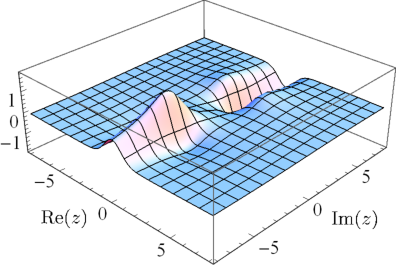
\includegraphics[scale=1]{4-Potentials/Figures/figure4Ba.pdf}
  }
  &
  \subfloat[$\Im \left( \frac{\partial \Vg(\vbr)}{i \, \partial \Im(z)} \right)$]{
    \label{f4-cauchy-riemann-for-numerical-gaussian-b}
    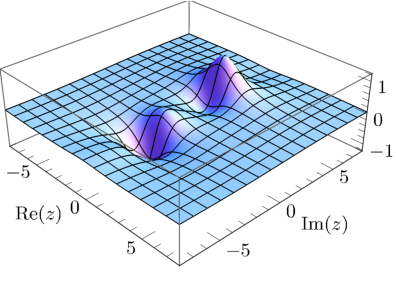
\includegraphics[scale=1]{4-Potentials/Figures/figure4Bb.pdf}
  }
  \\
  \subfloat[$\Re \left( \frac{\partial \Vg(\vbr)}{\partial \Re(z)} \right) \approx \Re\left( \frac{\partial \Vg(\vbr)}{i \, \partial \Im(z)} \right)$]{
    \label{f4-cauchy-riemann-for-numerical-gaussian-c}
    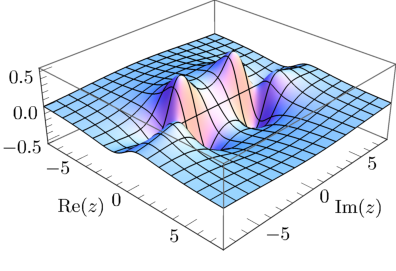
\includegraphics[scale=1]{4-Potentials/Figures/figure4Bc.pdf}
  }
  &
  \subfloat[$\left| \frac{\partial \Vg(\vbr)}{\partial \Re(z)} - \frac{\partial \Vg(\vbr)}{i \, \partial \Im(z)} \right|$]{
    \label{f4-cauchy-riemann-for-numerical-gaussian-d}
    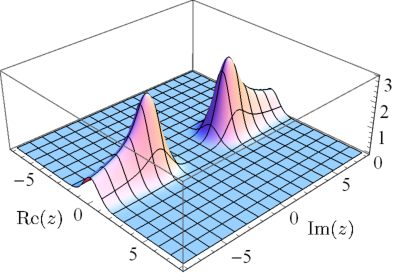
\includegraphics[scale=1]{4-Potentials/Figures/figure4Bd.pdf}
  }
  \end{tabular}
  \caption[Cauchy-Riemann equations for the numerically-integrated dlectrostatic potential $\Vg(\vbr)$ over complex coordinates]{
  Cauchy-Riemann equations for the numerically-integrated electrostatic potential $\Vg(\vbr)$ of \eqref{e4-correlation-interaction-potential-numerically-gaussian}, shown over the same slice of complex coordinate space as \reffig{f4-numerical-potential-from-gaussian} ($x=3$, $y=0$, and complex $z$).
  Panels~\protect\subref{f4-cauchy-riemann-for-numerical-gaussian-a} and~\protect\subref{f4-cauchy-riemann-for-numerical-gaussian-b} show the imaginary parts of the derivative of $\Vg(\vbr)$ with respect to the real and imaginary parts of $z$, respectively; for an analytical function they should match but instead they have immediately appreciable differences. The real parts, shown in~\protect\subref{f4-cauchy-riemann-for-numerical-gaussian-c}, do match, but the two derivatives are left with a strong difference, shown in~\protect\subref{f4-cauchy-riemann-for-numerical-gaussian-d}.
  }
  \label{f4-cauchy-riemann-for-numerical-gaussian}
\end{figure}
\captionsetup[figure]{position=auto}



The reason for why $\Vg(\vbr)$ fails to be analytical can be seen, at least after the fact, from its integral form \eqref{e4-correlation-interaction-potential-with-complex-position}. There, when we write
\begin{align}
\Vg(\vbr)
& =
\int\!
\frac{
  \normg \exp(-r'^2/\sigma^2)
  }{
  \sqrt{ \left( \vbr-\vbr' \right)^2}
  }
\d\vbr'
,
\label{e4-correlation-interaction-potential-for-analyticity}
\end{align}
we are expressing $\Vg(\vbr)$ as a continuous superposition of Coulombic point-charge potentials $1/\sqrt{ \left( \vbr-\vbr' \right)^2}$, and these are not analytic when $\vbr'$ lies in the circular singularity, as described by \eqref{e4-circular-singularity}, with respect to $\vbr$. Since the integral always includes points $\vbr'$ at this singularity and its neighbourhood, the assumption of analyticity of the resulting integral should be seen as suspect from the~start.







\section{Exactly integrable potentials}
We see, then, that the formulation of our correlation interaction potential $\Vnm{\vbr}$ as an integral over the ionic electrons' positions must be reformulated from its foundations when the probe point $\vbr$ is complex-valued. This is somewhat problematic, since we initially defined $\Vnm{\vbr}$ as the matrix element 
\begin{equation}
\Vnm{\vbr}=\matrixel**{n}{\sum_{j=1}^{N-1} \frac{1-\delta_{nm}}{\| \vbr - \hat{\vbr}_j\|} }{m}
\backtag{e4-correlation-interaction-potential-initial}
\end{equation}
at the start of this chapter, and there are few ways of evaluating such matrix elements that don't rely on an integral. 

However, a more careful analysis shows that the matrix element \eqref{e4-correlation-interaction-potential-initial} is only needed when defining $\Vnm{\vbr}$ for real-valued positions, since that is what goes into the original temporal integral for the ionization yield in \eqref{e2-correlation-driven-yield-separated} and \eqref{e2-correlation-driven-yield-with-eva-states}, and the only thing we need is the analytical continuation of this $\Vnm{\vbr}$ -- obtained by any reasonable means~-- when we shift the endpoint of the temporal integral into the complex plane to arrive at~\eqref{e2-correlation-driven-yield-semi-final}. 


This would seem to offer a very small comfort, since constructive theorems on analytical continuation are few and far between, but fortunately for us our problem has plenty of structure that we can exploit. To begin with, for many of the charge densities $\rho(\vbr)$ that we care about, including gaussian and exponential charge densities, the electrostatic potential, obtained as
\begin{align}
V(\vbr)
& =
\int\!
\frac{
  \rho(\vbr') \:\d\vbr'
  }{
  \sqrt{ \left( \vbr-\vbr' \right)^2}
  }
,
\label{e4-electrostatic-potential-as-integral}
\end{align}
can actually be integrated exactly in terms of a closed elementary expression -- and, when this is possible, the elementary expression gives an automatic analytical continuation. In fact, it isn't even necessary to do a full integration, since the integral electrostatic potential in \eqref{e4-electrostatic-potential-as-integral} can  be described equally well, for real positions, as the unique solution of the Poisson equation
\begin{equation}
\nabla^2 V(\vbr)=-4\pi \rho(\vbr)
\label{e4-poisson-equation}
\end{equation}
under $V(\vbr)\to 0$ as $|\vbr|\to\infty$. In fact, for spherically symmetric charge distributions, this reduces to a simple second-order ordinary differential equation, which is much easier to integrate, and additional angular-momentum polynomial factors can also be accommodated rather easily by suitable modifications of the spherically-symmetric case.

This means, then, that for the gaussian charge distribution \eqref{e4-gaussian-charge-density} that proved so problematic earlier we can simply write down the potential as
\begin{subequations}
\label{e4-exact-gaussian-potential}
\begin{align}
\Vg(\vbr) 
& = 
\pi^{3/2} \sigma^3 \normg \frac{ \erf(r/\alpha) }{ r }
\\ & = 
Q \frac{ \erf(r/\alpha) }{ r }
,
\end{align}
\end{subequations}%
in terms of a simple error function \citenistchap{7} and the total charge $Q$. Similarly, with the other building block of quantum chemical bases, the Slater-type orbital with an exponential charge density
\begin{equation}
\rhoe(\vbr) = \norme \exp(-r/\sigma)
,
\label{e4-exponential-charge-density}
\end{equation}
the radial Poisson equation can also be trivially solved to give the potential
\begin{subequations}
\label{e4-exact-exponential-potential}%
\begin{align}
\Ve(\vbr) 
& = 
4\pi \alpha^2 \norme \left[ - \left( 1 + \frac{2\alpha}{r} \right) e^{-r/\alpha} + \frac{2\alpha}{r} \right]
\\ & = 
 \frac{Q}{2\alpha} \left[ - \left( 1 + \frac{2\alpha}{r} \right) e^{-r/\alpha} + \frac{2\alpha}{r} \right]
.
\end{align}%
\end{subequations} %

It is important to note that both of these exact potentials were obtained by integrating Poisson's equation \eqref{e4-poisson-equation} for real coordinates, and they are only equal to the integrally-defined potential \eqref{e4-electrostatic-potential-as-integral} when $\vbr$ is real. However, both exact formulas \eqref{e4-exact-gaussian-potential} and \eqref{e4-exact-exponential-potential} \textit{must} hold for the analytical continuation of \eqref{e4-electrostatic-potential-as-integral} into complex-valued $\vbr$, because for each coordinate they coincide on the real axis, and that is sufficient to ensure the uniqueness of the analytical continuation. Since the both \eqref{e4-exact-gaussian-potential} and \eqref{e4-exact-exponential-potential} are analytic, they are \textit{the} unique extension of \eqref{e4-electrostatic-potential-as-integral} to the complex plane \cite[\S108]{churchill_complex_variables}.


\vspace{5mm}


\begin{mathaside}{Analytical continuation}
\label{aside.analytical-continuation}

At this point, it is worth spending some time emphasizing this feature of the theory of complex variables. If we are given a function $f:\mathbb{R}\to \mathbb{C}$ which is `nice enough', it is usual to speak of its analytical continuation as if this extension of $f$ to the complex plane can always be done, and can always be done uniquely. The possibility and uniqueness of analytical continuation in a multiply connected region is a complicated question, which reaches fruition in the theory of Riemann surfaces. (On the other hand, it is all too common to assume that, multivaluedness issues aside, any analytical function can always be extended as far as necessary, which need not be the case: many functions run into natural boundaries, which stop any kind of analytical continuation~\cite[p.~191]{noguchi_complex_analysis}.)

\vspace{\maskip}
In our context, it is worth emphasizing just how little is really necessary to ensure the uniqueness of an analytical continuation; the standard result \cite[given e.g. in Ref.][pp.~283ff]{churchill_complex_variables} is usually stated in the form

\begin{theorem}
A function that is analytic in a domain $D$ is uniquely determined over $D$ by its values over a subdomain, or along an arc, interior to $D$.
\end{theorem}


where the key word is the concept of a \textit{domain}, which is restricted to an open, singly connected subset $D$ of $\mathbb{C}$. However, the hypotheses for this usual statement can be softened considerably \cite[p.~95]{noguchi_complex_analysis}: the agreement over a line can be loosened to agreement over a sequence $(s_n)_{n=0}^\infty \subset D$ that converges to a point $s_n\to s\in D$, or, in other words,
%%% also http://www.unc.edu/math/Faculty/met/complex.pdf

\begin{theorem}
A function that is analytic in a domain $D$ is uniquely determined over $D$ by its values on any set $S\subset D$ which has an accumulation point in $D$.
\end{theorem}


This is, again, an expression of the rigidity of the theory of analytical functions, especially when compared to the study of continuously differentiable real functions, where no similar result is even remotely true. Complex analytical functions, being the solutions of a differential equation, are much more constrained by their values on the boundary or subparts of a domain.

\end{mathaside}




Now that we have suitable analytical continuations of at least some reasonable charge distributions, the next thing to investigate is their behaviour as functions of $\vbr$. The first thing to try is to look at their behaviour over real coordinates, and here both potentials look remarkably similar (modulo some leeway on how to relate the $1/e$ widths $\sigma$ and $\alpha$ of the two charge distributions), as shown in \reffig{f4-exact-gaussian-vs-exponential-real-coordinates}. 

\begin{figure}[htb]
  \centering
  \begin{tabular}{c}
  \subfloat{  
    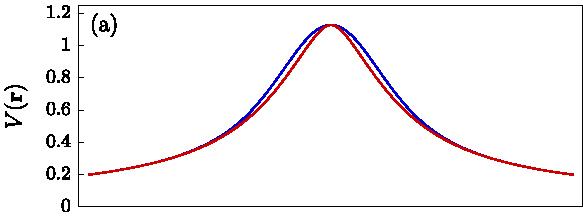
\includegraphics[scale=1]{4-Potentials/Figures/figure4Ca.pdf}
    \label{f4-potential-comparison} 
  }
  \\[-5mm]
  \subfloat{
    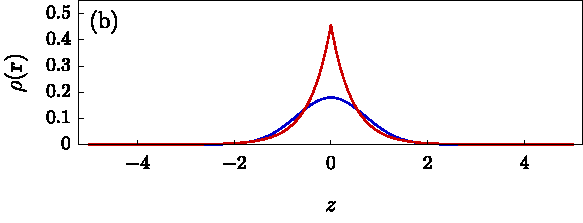
\includegraphics[scale=1]{4-Potentials/Figures/figure4Cb.pdf}
    \label{f4-charge-density-comparison} 
  }
  \end{tabular}
  \caption[Exact electrostatic potentials $\Vg(\vbr)$ and $\Ve(\vbr)$, for gaussian and exponential charge densities, over real coordinates]{
  Exact electrostatic potentials $\Vg(\vbr)$ (blue) and $\Ve(\vbr)$ (red) as a function of real coordinates, for equal total charges $Q=1$ and with the $1/e$ widths $\sigma=1$ and $\alpha=\sqrt{\pi}/4$ chosen so the potentials will match at the origin. The corresponding charge distributions are shown~in~\protect\subref{f4-charge-density-comparison}.}
  \label{f4-exact-gaussian-vs-exponential-real-coordinates}
\end{figure}


In general, gaussian distributions are rather different to Slater-type exponential orbitals, because they lack the latter's cusp at the origin, and they have markedly thinner tails at the edges. Nevertheless, if we relate the two widths by asking that the potential at the origin $V(\mathbf 0)$ be the same for both distributions, we get relatively similar charge distributions, as shown in \reffig{f4-charge-density-comparison}, and the remarkably similar electrostatic potentials of~\reffig{f4-potential-comparison}. Since the charge distributions are relatively similar blobs for both cases, we can hope that their potentials will also have similar behaviour for complex coordinates.






Unfortunately, the similarities between the two potentials end there, and when we look at their behaviour for complex coordinates we get completely different structure, shown in \reffig{f4-exact-gaussian-vs-exponential-complex-coordinates}.
% for the same cut through complex $\vbr$ space as in Figs.~\ref{f4-numerical-potential-from-gaussian} and \ref{f4-cauchy-riemann-for-numerical-gaussian} (i.e. taking a fixed $x=3$ and $y=0$ and varying $z\in\mathbb{C}$). 



\captionsetup[figure]{position=top}
\begin{figure}[htb]
  \centering
  \begin{tabular}{cc}
  \subfloat[$\Re(\Vg(\vbr))$]{
    \label{f4-re-vg-over-complex-coords}
    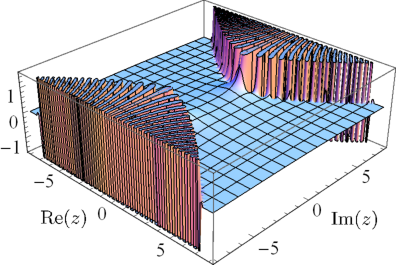
\includegraphics[scale=1]{4-Potentials/Figures/figure4Da.pdf}
  }
  &
  \subfloat[$\Im(\Vg(\vbr))$]{
    \label{f4-im-vg-over-complex-coords}
    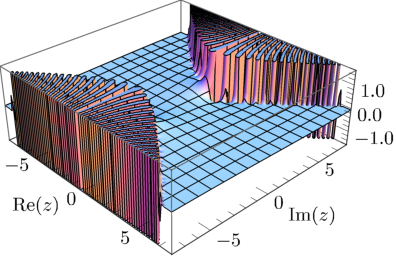
\includegraphics[scale=1]{4-Potentials/Figures/figure4Db.pdf}
  }
  \\[6mm]
  \subfloat[$\Re(\Ve(\vbr))$]{
    \label{f4-re-ve-over-complex-coords}
    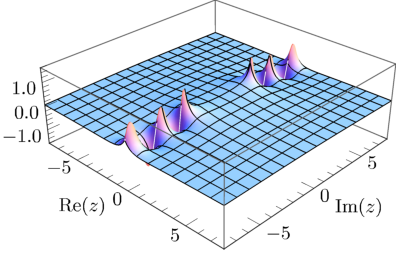
\includegraphics[scale=1]{4-Potentials/Figures/figure4Dc.pdf}
  }
  &
  \subfloat[$\Im(\Ve(\vbr))$]{
    \label{f4-im-ve-over-complex-coords}
    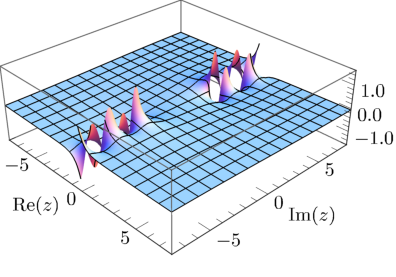
\includegraphics[scale=1]{4-Potentials/Figures/figure4Dd.pdf}
  }
  \end{tabular}
  \caption[Exact electrostatic potentials $\Vg(\vbr)$ and $\Ve(\vbr)$, for gaussian and exponential charge distributions, over complex coordinates]{
  Exact electrostatic potentials $\Vg(\vbr)$ and $\Ve(\vbr)$ over complex coordinates, with the same cut over complex space as Figs.~\ref{f4-numerical-potential-from-gaussian} and \ref{f4-cauchy-riemann-for-numerical-gaussian}. The potential $\Vg(\vbr)$ from a gaussian charge distribution diverges at imaginary coordinates, while the potential $\Ve(\vbr)$ from an exponential distribution has a branch cut there.
  }
  \label{f4-exact-gaussian-vs-exponential-complex-coordinates}
\end{figure}
\captionsetup[figure]{position=auto}


Perhaps the most salient feature of both of these potentials is the stark divergence of the exact gaussian potential $\Vg(\vbr)$ as the imaginary part of $z$ increases, which immediately becomes unmanageable regardless of the scale on the vertical axis. This can be seen quite clearly from the asymptotic expansion for the error function \citenisteq{7.12.1}, which at large and real argument describes a gaussian approach from below to 1, but inherits this $e^{-z^2}$ behaviour for the entire complex plane:
\begin{equation}
\erf(z) \sim 1 - \frac{e^{-z^2}}{\sqrt{\pi}} \left( 1- \frac{1}{z} + \frac{1}{2z^2} - \cdots \right)
\label{e4-erf-asymptotic-expansion}
\end{equation}
whenever $|\arg(z)| < \frac{3\pi}{4}$. In the potential $\Vg(\vbr)$ from \eqref{e4-exact-gaussian-potential}, the error function is called with $r=\sqrt{x^2+y^2+z^2}$ as an argument, which means that for large $|z|$ it behaves as $\exp((\Im(z)^2-\Re(z)^2)/\sigma^2)$, and if the imaginary part of $z$ is large enough then $\Vg(\vbr)$ will diverge in a super-gaussian fashion. This strong divergence is then responsible for the wall-like behaviour shown in Figs.~\ref{f4-re-vg-over-complex-coords} and \ref{f4-im-vg-over-complex-coords}. Finally, to add a slight insult to the injury, the complex exponential also oscillates ever more wildly in this region.



The potential for the exponential distribution, $\Ve(\vbr)$, on the other hand, has much more bounded behaviour, but instead of a divergence to infinity it now fills up its interestingness quota with a pair of branch cuts that stretch from $z=\pm i x$ to imaginary infinity. These branch cuts are, in fact, rather natural, because the potential is a function of $r=\sqrt{x^2+y^2+z^2}$, which itself has a sign-change branch cut when its argument is~negative. 
%%% In a sense, this branch cut is harder to deal with than the exponential divergence of $\Vg(\vbr)$, because integration contours cannot cross branch cuts


It is worth asking at this stage why the gaussian potential $\Vg(\vbr)$ does not exhibit any branch cuts on its domain: after all, it is a function of $r$ just as much as $\Ve(\vbr)$. The reason for this is that the error function is a pure odd function, and it therefore has a Taylor expansion \citenisteq{7.6.1} of the form
\begin{equation}
\erf(z)
%=\frac{2}{\sqrt{\pi}}\sum_{n=0}^{\infty} \frac{(-1)^{n}z^{2n+1}}{n!(2n+1)}
=\frac{2}{\sqrt{\pi}}\left( z - \frac{z^3}{3} + \frac{z^5}{10} - \cdots \right)
.
\end{equation}
This means, in turn, that the gaussian potential \eqref{e4-exact-gaussian-potential} also has a Taylor series of definite parity,
\begin{equation}
\Vg(\vbr) 
=
Q \frac{ \erf(r/\sigma) }{ r }
=
\frac{2Q}{\sqrt{\pi}\sigma}\left( 1 - \frac{r^2}{3\sigma^2} + \frac{r^4}{10\sigma^4} - \cdots \right)
,
\end{equation}
except that now $\Vg(\vbr)$ is a pure even function, so it is a function of $r^2$. Since $r^2$ has no branch cuts, $\Vg(\vbr)$ cannot have any either. It is this sort of subtle difference in the potentials' behaviour for real coordinates that causes the stark differences at complex coordinates shown in \reffig{f4-exact-gaussian-vs-exponential-complex-coordinates}.


The divergence in behaviour of our two potentials at complex coordinates is definitely worrisome, since they are both more or less reasonable models for real-world charge distributions. Gaussian and exponential-type orbitals are the general building blocks of quantum chemistry, and while they are certainly not interchangeable (with a definite conceptual advantage to exponential charges, since the gaussian distributions lack the cusps and long tails expected of real-world orbitals), as far as real-coordinates electrostatics is concerned they are both essentially blobs of charge that produce very similar electrostatic potentials. 


It is also important to note that this difference in behaviour is quite certain to persist through most of the common modifications to our model charge distributions. On the simplest level, the addition of polynomial factors to a gaussian charge is exactly equivalent to taking its derivatives, which means that the overall (super-)gaussian factor will always be present. A similar, more involved argument holds for exponential orbitals.

On a slightly higher level, it is also impossible to get radically different behaviour from any finite collection of gaussians, since the linearity of Poisson's equation implies that the potential will be the corresponding linear combination of $\Vg(\vbr)$'s, and it is essentially impossible for such a function to be well-behaved everywhere, since it is an entire function and we know it decays as $1/r$ or faster in all real directions, so it needs to diverge to infinity at large imaginary coordinates. 

Moreover, the behaviour at large imaginary coordinates will be dominated by the contributions from the tightest gaussians in the basis set, because these will have the shortest length scales $\sigma$, and that means that their corresponding potentials $\Vg(\vbr)\sim \exp(+\Im(\vbr)^2/\sigma^2)$ will be the fastest to explode. While there will probably be at least two of these at the same width, they are overwhelmingly unlikely to contribute in such a way that their divergences will cancel out, especially when probed over all possible lines on real space and all possible directions in the complex continuation of that real cut.  This argument, moreover, extends to transition charges that integrate to zero total charge.



Given that $\Vg(\vbr)$ and $\Ve(\vbr)$ produce wildly different potentials for complex coordinates, we are now left with the even bigger question of what should be the general features to expect of the complex-coordinates electrostatic potential $V(\vbr)$ for a realistic charge distribution -- should it have branch cuts? should it diverge exponentially? super-exponentially? should it have poles, while we're at this? -- and we are left with precious few tools to answer this question.



\captionsetup[figure]{position=top}
\begin{figure}[!htbp]
  \centering
  \begin{tabular}{cc}
  \subfloat[$\Re(\Vg(\vbr))$]{
    \label{f4-potentials-comparison-restricted-complex-coordinates-a}
    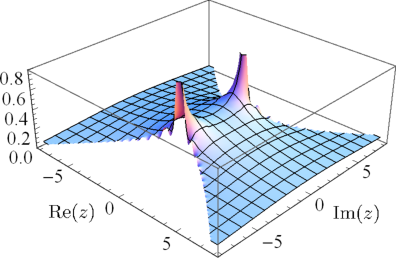
\includegraphics[scale=1]{4-Potentials/Figures/figure4Ea.pdf}
  }
  &
  \subfloat[$\Im(\Vg(\vbr))$]{
    \label{f4-potentials-comparison-restricted-complex-coordinates-b}
    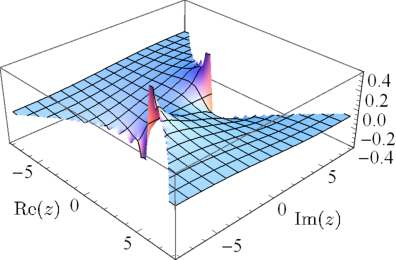
\includegraphics[scale=1]{4-Potentials/Figures/figure4Eb.pdf}
  }
  \\
  \subfloat[$\Re(\Ve(\vbr))$]{
    \label{f4-potentials-comparison-restricted-complex-coordinates-c}
    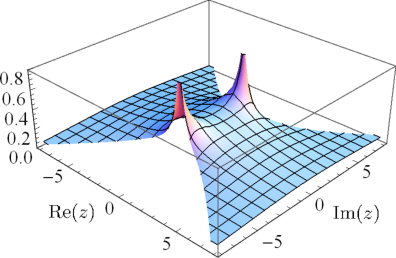
\includegraphics[scale=1]{4-Potentials/Figures/figure4Ec.pdf}
  }
  &
  \subfloat[$\Im(\Ve(\vbr))$]{
    \label{f4-potentials-comparison-restricted-complex-coordinates-d}
    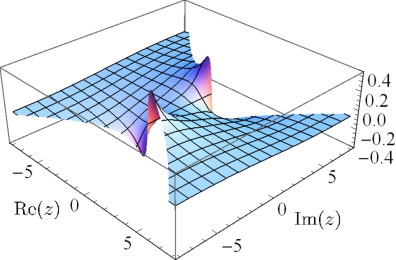
\includegraphics[scale=1]{4-Potentials/Figures/figure4Ed.pdf}
  }
  \\
  \subfloat[$\Re(\Vgnum(\vbr))$]{
    \label{f4-potentials-comparison-restricted-complex-coordinates-e}
    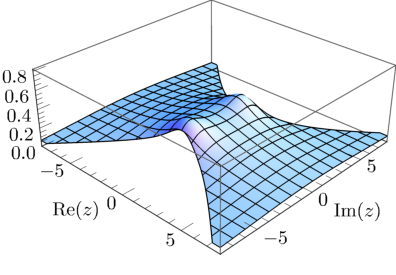
\includegraphics[scale=1]{4-Potentials/Figures/figure4Ee.pdf}
  }
  &
  \subfloat[$\Im(\Vgnum(\vbr))$]{
    \label{f4-potentials-comparison-restricted-complex-coordinates-f}
    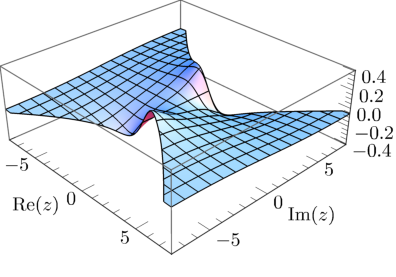
\includegraphics[scale=1]{4-Potentials/Figures/figure4Ef.pdf}
  }
  \end{tabular}
  \caption[Electrostatic potentials $\Vg(\vbr)$, $\Ve(\vbr)$ and $\Vgnum(\vbr)$ over complex coordinates restricted to $\Re(\vbr^2)>0$]{
  Exact electrostatic potentials $\Vg(\vbr)$ and $\Ve(\vbr)$ over complex coordinates (\subref*{f4-potentials-comparison-restricted-complex-coordinates-a}-\subref*{f4-potentials-comparison-restricted-complex-coordinates-d}), exactly as in \reffig{f4-exact-gaussian-vs-exponential-complex-coordinates}, but restricted to the region $\Re(\vbr^2)>0$. Despite their disagreements in coordinates that are `too imaginary' (in the sense that $\Re(\vbr^2)=\Re(\vbr)^2-\Im(\vbr)^2<0$), both potentials agree quite well here. (We show their close quantitative agreement in \reffig{f4-quantitative-agreements-between-potentials}.) In addition, they also agree relatively well (particularly when away from the boundary) with the numerically-integrated $\Vgnum(\vbr)$ of Section~\ref{sec:quantum-chemical-potentials-complex}, shown in~\subref{f4-potentials-comparison-restricted-complex-coordinates-e} and~\subref{f4-potentials-comparison-restricted-complex-coordinates-f}; this means that $\Vgnum(\vbr)$ is also a relatively reasonable model in that~region, though its much higher computational cost and worse analyticity properties render it a bad choice.}
  \label{f4-potentials-comparison-restricted-complex-coordinates}
\end{figure}


The one saving grace of this problem is that the differences in behaviour are confined to very identifiable regions in complex $\vbr$ space. The complex-coordinates electrostatic potentials shown in \reffig{f4-exact-gaussian-vs-exponential-complex-coordinates} look very different, but this masks somewhat the fact that, if you ignore the regions where $\Vg(\vbr)$ behaves wildly, then the two potentials actually agree rather closely, both qualitatively and quantitatively. The regions where this happens are easily pointed out through the asymptotic expansion \eqref{e4-erf-asymptotic-expansion} for $\erf(r/\sigma)$, which makes it clear that, as long as
%
\begin{equation}
\Re(\vbr^2)>0,
\label{e4-re-r2-less-than-0}
\end{equation}
%
then the exponential term is decaying and $\Vg(\vbr)$ should be well-behaved. As we shall see, the restriction \eqref{e4-re-r2-less-than-0} will be a driving consideration hereafter.

In the meantime, we can begin by looking at the potentials we have so far when restricted to this region, and these are shown in \reffig{f4-potentials-comparison-restricted-complex-coordinates}. Once the region with the $\Vg(\vbr)$ divergence, and the $\Ve(\vbr)$ branch cut, is removed, both potentials have essentially the same shape, and indeed even quantitatively match to a remarkable degree, as shown in \reffig{f4-quantitative-agreements-between-potentials}. Even more notably, both exact potentials also show a good match to the numerically-integrated $\Vg(\vbr)$ in this~region.



\captionsetup[figure]{position=top}
\begin{figure}[!htbp]
  \centering
  \begin{tabular}{cc}
  \subfloat[$|\Ve(\vbr)-\Vg(\vbr)|/|\Vg(\vbr)|$]{
    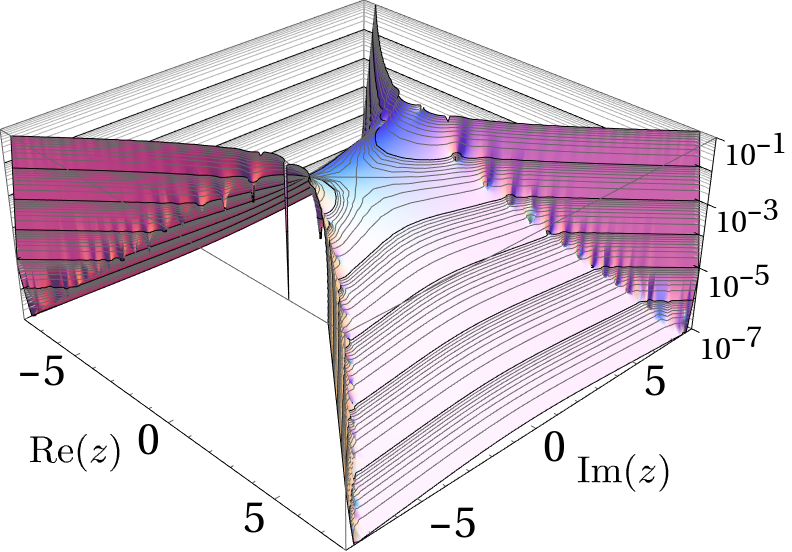
\includegraphics[scale=1]{4-Potentials/Figures/figure4Fa.png}
  }
  &
  \subfloat[$|\Vgnum(\vbr)-\Vg(\vbr)|/|\Vg(\vbr)$]{
    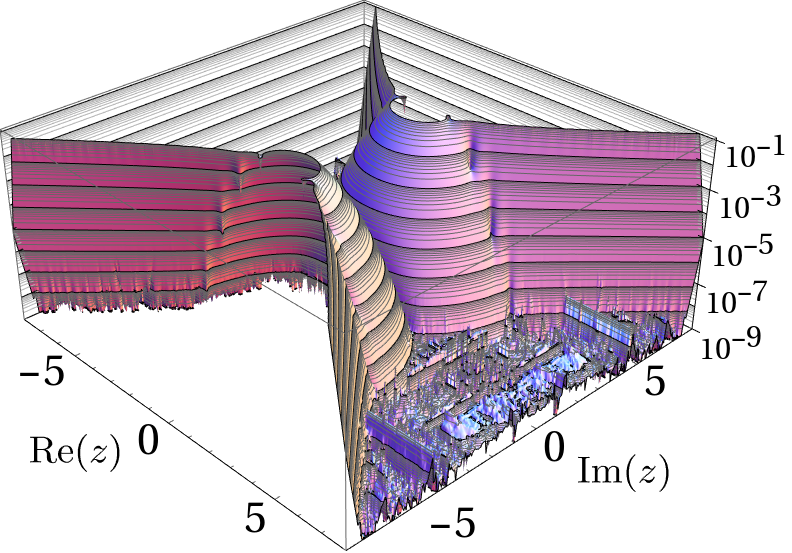
\includegraphics[scale=1]{4-Potentials/Figures/figure4Fb.png}
  }
  \end{tabular}
  \caption[Residuals between the electrostatic potentials $\Ve(\vbr)$ and $\Vg(\vbr)$, from exponential and gaussian charges, and $\Vgnum(\vbr)$ and $\Vg(\vbr)$ from numerical and exact integration for a gaussian charge, showing agreement where $\Re(\vbr^2)>0$]{
  Normalized differences between the exponential-charge potential $\Vg(\vbr)$ and the exact gaussian potential $\Vg(\vbr)$ as a reference (a), and the numerically-integrated potential $\Vgnum(\vbr)$ of section \ref{sec:quantum-chemical-potentials-complex}, against $\Vg(\vbr)$ (b), on a logarithmic scale. The plots use the same cut over complex space as Figs.~\ref{f4-numerical-potential-from-gaussian}, \ref{f4-cauchy-riemann-for-numerical-gaussian}, \ref{f4-exact-gaussian-vs-exponential-complex-coordinates} and \ref{f4-potentials-comparison-restricted-complex-coordinates} and are (roughly) restricted the allowed region $\Re(\vbr^2)>0$ of~\eqref{e4-re-r2-less-than-0}. The agreement here is not only qualitatively good, as shown in \reffig{f4-potentials-comparison-restricted-complex-coordinates}, but also quantitatively rather close, with the potentials agreeing to better than 1\% over large regions. On the other hand, once the mostly-imaginary region $\Re(\vbr^2)<0$ is reached, the disagreement rises very steeply.
  }
  \label{f4-quantitative-agreements-between-potentials}
\end{figure}




On the other hand, the close match between the potentials in the region $\Re(\vbr^2)>0$ is also a cause for concern, because it carries no warning of the wild disagreements that sprout between them with alarming speed upon leaving this region. If one is using some local method to extend the domain of the electrostatic potential, for example, how is one to detect and handle a sudden, catastrophic blow-up in the potential? It bears emphasizing that the remarkably similar surfaces shown in \reffig{f4-quantitative-agreements-between-potentials} are solutions of the \textit{same} rigid differential equation discussed in the Mathematical Aside~\ref{aside.analytical-continuation} -- a differential equation which enforces the uniqueness of its solutions over their entire domains when given (exact) agreement even at a single accumulation point -- and yet these solutions can still depart from each other, suddenly and steeply, as in \reffig{f4-exact-gaussian-vs-exponential-complex-coordinates}.


Given all of this, can we say that both $\Vg(\vbr)$ and $\Ve(\vbr)$ have the ``right'' shapes in the region where $\Re(\vbr^2)>0$, if their minute differences can lead to wildly different behaviour at a moment's notice? If it is possible to talk about a ``correct'' shape, which one is it? If both can be right depending on circumstances, which one should we use to set expectations for the physical charge density in a real-world molecule?






\section{Outlook}
In the end, unfortunately, none of these questions have any easy answers. Simply put, the theory of analytical functions is just too rigid, and depends too delicately on the initial boundary values, to say anything of consequence about the global behaviour of a general electrostatic potential $V(\vbr)$ over the entirety of complex $\vbr$ space, and the overall recommendation is to stay, whenever possible, in the `safe' region
\begin{equation}
\Re(\vbr^2)>0,
\backtag{e4-re-r2-less-than-0}
\end{equation}
where the different approaches agree.

One might also ask, at this point, for what evidence we have that the problem is even solvable: to what extent do we know that there even exists an analytical continuation for the electrostatic potential $V(\vbr)$ of a generic real-world (transition) charge density $\rho(\vbr)$? Here (regardless of whether this is fortunate or unfortunate) the answer is positive: in general, this analytical continuation does exist, at least for some open set about the real~slice of complex $\vbr$ space.


The reason for this is that the electrostatic potential $V(\vbr)$ is a solution of the Poisson equation~\eqref{e4-poisson-equation}, and it therefore gets many of its properties from the robust structure of the Laplacian operator; more specifically, the Laplacian is required to have analytic solutions whenever the right-hand side is analytic. Similarly, this right-hand-side function $\rho(\vbr)$ is obtained from the eigenfunctions of the time-independent Schrödinger equation on multiple dimensions,%
\footnote{%
This does entail a nontrivial step in showing that an analytical solution of the Schrödinger equation give an analytical charge density, since expressions of the form $\phi_m(\vbr)^* \phi_n(\vbr)$ include a complex conjugation that can destroy the analyticity if not done correctly. Fortunately, this can be done easily by extending functions of the form $\phi_m(\vbr)^*$ to the complex plane as $\phi_m(\vbr^*)^*$, which is analytic by the Schwarz reflection principle~\cite[p.~119-120]{noguchi_complex_analysis}.
}
% (admittedly through a procedure that can involve an analyticity-denying conjugation in $\phi_m(\vbr)^* \phi_n(\vbr)$, which can nevertheless be factored away as the eigenfunctions can always be chosen to be real), 
and again the Schrödinger multi-electron Hamiltonian is generally regular enough that its eigenfunctions are analytic.



\begin{mathaside}{Analytic regularity of elliptic operators}
\label{aside.elliptic-regularity}

As a final building block of the mathematics that underpins this chapter, it is also worth detailing the results that guarantee the existence of the analytical continuations of the electrostatic potentials $V(\vbr)$ that we need. The main such result is the Elliptic Regularity Theorem, which governs the regularity of solutions of elliptic partial differential equations; it can be phrased in a number of ways but a suitably strong one is provided by L. Hörmander in \citer{hormander_pdes}, p.~178, as the following theorem:

\begin{theorem}
Let $P(x, D)$ be an elliptic differential operator in $D$ with coefficients that are analytic in $D$. If $u\in \mathscr D'(\Omega)$ and 
\begin{equation}
P(x, D)u = f 
\end{equation}
where $f$ is also analytic in $\Omega$, then $u$ is analytic in $\Omega$. 
\end{theorem}


Here $\mathscr D'(\Omega)$ denotes the set of all distributions over $\Omega$ (formally defined as a set of suitably bounded linear functionals $u\colon C_0^\infty(\Omega) \to \mathbb{C}$), but the requirement that $f$ and $u$ be analytical turns them into regular functions over $\Omega$ and fulfils the boundedness condition on the distribution. %\\[-8pt]

%
%Theorems of this form, guaranteeing differentiability properties of the solution $u$ to a partial differential equation $P(x,D)u=f$ with a well-behaved right-hand side $f$, are generally known as regularity theorems, and they typically hold strictly for elliptic operators. In particular, the Elliptic Regularity Theorem guarantees a smooth solution to elliptic PDEs whenever the right-hand side is smooth, and in general operators with this property are called hypoelliptic. Similarly, the stronger requirement of analytical solutions to analytical initial data is termed analytic hypoellipticity.

\vspace{\maskip}
In particular, both the Schrödinger and the Poisson equations are of this form (once one excludes the Coulomb singularities), since they are both elliptic and have analytical coefficients and right-hand sides, so both are required to have analytical solutions.

\end{mathaside}



We have, then, the promise from an existence theorem that, given an idealized real-world (transition) charge density $\rho(\vbr)$, there should be a Platonic `true' analytical continuation of the relevant electrostatic potential $V(\vbr)$: the multi-electron Hamiltonian has analytical true eigenfunctions, which combine into an analytical charge density, and this then gives an analytical electrostatic potential. However, we have no way to find this `true' potential (which is relatively reasonable, as we cannot even find the true eigenfunctions) or even have any idea of what it should behave like, let alone find reasonable approximations for it (and this does break the usual paradigms).

One could think, for example, that to find an analytical continuation it would hopefully be good enough to find chemical data for the charge density and the electrostatic potential for real coordinates which was accurate enough, and then if necessary perform a numerical solution of the Cauchy-Riemann equations for these data. Unfortunately, such an effort is doomed to fail: the numerical solution of the Cauchy-Riemann problem is likely to prove a stiff, unstable problem, because -- as demonstrated in Figs.~\ref{f4-potentials-comparison-restricted-complex-coordinates} and \ref{f4-exact-gaussian-vs-exponential-complex-coordinates} -- very similar initial conditions can lead to very sudden, unexpected divergences, even for exactly-known potentials.

Moreover, even if we \textit{could} somehow perform this numerical solution of the Cauchy-Riemann equations to arbitrary accuracy over the entire complex plane, we would still be left with the wrong solution. This is because the quantum chemical data, in the end, produces a charge density $\rho(\vbr)$ which is ultimately a sum of gaussian-type distributions. To be sure, these will come in many places and sizes, to approximate to high accuracy the long tails and the sharp cusps of the expected real-world distribution, but in the end it will still be a finite superposition of gaussians, and the exact solution will still be the corresponding finite superposition of~$\Vg(\vbr)$s. 

Thus, it is conceivable that we could succeed in numerically solving the Cauchy-Riemann problem to accuracy close enough to the exact solution -- but we already know what this exact solution looks like: it is the relevant superposition of gaussian potentials $\Vg(\vbr)$ from \eqref{e4-exact-gaussian-potential}, and we know that these potentials diverge when $\Re(\vbr^2)<0$ as shown in~\reffig{f4-exact-gaussian-vs-exponential-complex-coordinates}, and that they do not match the exponential model which is more physically reasonable.

Similarly, one might hope that for a real molecule these divergences would cancel out in some way, but as we have seen, this is very unlikely. Instead, large $\Im(\vbr)$ any superposition-of-$\Vg(\vbr)$s potential will be dominated by the contribution from the smallest gaussians, which are typically used to approximate the cusps at the nuclei, since these will have the shortest length scales $\sigma$, and therefore their corresponding potentials $\Vg(\vbr)\sim \exp(+\Im(\vbr)^2/\sigma^2)$ will be the fastest to explode.


Even worse, the close match between $\Ve(\vbr)$ and $\Vg(\vbr)$ in the allowed region bodes ill for any finitary approach to the potential through the charge distribution. To see this, suppose that we are given a guarantee of a uniform approximation to the Platonic charge density $\rho(\vbr)$, represented as a finite sum of manageable charge densities $\rho_i(\vbr)$. This is a rather reasonable thing to assume, and it is attained, for example, when solving for $\rho(\vbr)$ through Slater-type quantum chemical methods, which offer guarantees of the form $\left|\rho(\vbr)-\sum_i\rho_i(\vbr)\right|<\eps$, where $\eps$ is a numerical precision that can be set arbitrarily small (with a corresponding increase in the size and complexity of $\sum_i\rho_i(\vbr)$), and moreover the approximation is guaranteed for \textit{all} positions $\vbr$. Even a situation this ideal, however, fails to exclude the possibility that the Platonic charge density be equal to $\rho(\vbr) = \sum_i\rho_i(\vbr) + \eps'\rho_g(\vbr)$: the manageable numerical $\sum_i\rho_i(\vbr)$, with a small gaussian addendum $\eps'\rho_g(\vbr)$ which is bounded below $\eps$ for all real positions, but which will still quickly dominate the potential at imaginary positions that are large enough.



This therefore means that, although exponential charge densities are probably the most physically correct models for the Platonic charge distribution -- the one obtained mathematically from the regularity of the Schrödinger equation --, there is still uncertainty as to how well they extend to the complex plane. 

More mathematically, this means that while analytical continuation is possible and exact when we know the exact function we want to continue analytically, the use of finitely accurate data on a limited number of sample points to attempt an analytical continuation to the whole of the complex plane is, in the absence of very strict guarantees on the function we're approximating, bound to fail at least some of the time.




We see, then, that roughly half of complex $\vbr$ space is closed to the means of inquiry we have available to us, and we need to stay in the allowed region if we want to have meaningful electrostatic potentials from our transition charges.

However, in contrast with the bleak landscape presented above, the assumption of an exponential charge is in fact fairly reasonable, and the remarkably close agreement between the potentials as displayed in \reffig{f4-potentials-comparison-restricted-complex-coordinates} is a very encouraging sign that, within the allowed region, it is actually quite reasonable to assume that we've got the correct potential, even if we're using gaussian-based quantum chemical charge distributions.

Moreover, we also have a very clean criterion -- whether $\Re(\vbr^2)>0$ or not -- to tell whether we are in the allowed region, and we can use this information to help shape the complex-space trajectory $\rl(t)$ that we will actually use to probe the potential. In addition to this clear bound, in the next chapter we will show that it is in fact possible to choose the integration path in the complex time plane in a way that keeps the position-space trajectory completely within the allowed region, and that therefore the problematic cases never arise. 

In other words, the semiclassical quantum mechanics of complex-valued trajectories need to be handled carefully, and we have seen the serious breakdowns that can occur when one pushes too far, but we can also be fairly confident that within the bounds that we have described the behaviour will be manageable, and we will show in chapter~\ref{chap:quantum-orbits} how to ensure that the trajectory remains within those bounds.


Finally, and as an added bonus, we also get that as long as we stay in the allowed region, we can safely use the exact potentials $\Vg(\vbr)$ for each of the gaussian building blocks of any quantum chemical charge distributions, and this spares us the need of any numerical integration (which was ultimately doomed to produce non-analytical results in the first place), which therefore considerably speeds up the calculations of the ARM correlation-driven ionization yield, since we now require only a few queries of the $\Vg(\vbr)$ per temporal integration point, instead of iterating over a full numerical integration.


































   



\chapter[Quantum orbits as trajectories through complex time and complex\texorpdfstring{\\}{} space]{Quantum orbits as trajectories through complex time and complex space}
\label{chap:quantum-orbits}
\chaptermark{Quantum orbits as trajectories through complex time and complex space}

This chapter examines in closer detail the structure of the complex-valued electron trajectories used by the Analytical $R$-Matrix theory of photoionization: where it comes from, what the complex-valuedness means, how it interacts with the correlation interaction and the mean-field Coulomb potentials, under what circumstances the imaginary part becomes problematic, and how it should be handled in those conditions. 

We have built, in chapter~\ref{chap:R-matrix}, the framework for a semiclassical, trajectory-based theory of photoionization including the Coulomb and correlation interaction potential, building from the Schrödinger equation to obtainthe laser-driven trajectory
\begin{equation}
\rl(t) = \int_{\ts}^{t} \left[\vbp+\vba(\tau) \right] \: \d\tau
\label{e5-laser-driven-trajectory}
\end{equation}
as a fundamental object, and we have examined  the correlation interaction potentials that should be evaluated at this trajectory -- the reduction of the geometrical integrals to single evaluations of the potential in chapter~\ref{chap:multi-channel} and the properties of realistic and model molecular correlation interaction potentials when taken over complex coordinates in chapter~\ref{chap:complex-space-potentials}. Now we turn to the detailed properties of the laser-driven trajectory \eqref{e5-laser-driven-trajectory}.




The material in this chapter has appeared previously in reference
\begin{enumerate}
\item[{\hypersetup{citecolor=black}\citealp{Pisanty_slalom_2016}}.]
\textsc{E.~Pisanty and M.~Ivanov}.
\newblock Slalom in complex time:\ emergence of low-energy structures in tunnel
  ionization via complex time contours.
\newblock \href{http://dx.doi.org/10.1103/PhysRevA.93.043408}{
          \emph{Phys. Rev. A} \textbf{93} no.~4, p.~043\,408 (2016)}.
\newblock \href{http://arxiv.org/abs/1507.00011}{{arXiv}:1507.00011}.
\end{enumerate}
%
%
This chapter also describes work that is implemented in the software packages
\begin{enumerate}
\item[{\hypersetup{citecolor=black}\citealp{ARMSupport}}.]
\textsc{E.~Pisanty}.
\newblock {ARMSupport}: {A} support suite for {A}nalytical {$R$}-{M}atrix
  calculations.
\newblock \url{https://github.com/episanty/ARMSupport} (2016).

%\item[{\hypersetup{citecolor=black}\citealp{EPToolbox}}.]
%\textsc{E.~Pisanty}.
%\newblock {EPToolbox}.
%\newblock \url{https://github.com/episanty/EPToolbox} (2016).

\item[{\hypersetup{citecolor=black}\citealp{QuODD}}.]
\textsc{E.~Pisanty}.
\newblock {QuODD}: Quantum Orbits Dynamic Dashboard.
\newblock \url{https://github.com/episanty/QuODD} (2015).
\end{enumerate}


\vfill



\section[Emergence of complex-valued trajectories in Analytical R-Matrix theory]{Emergence of complex-valued trajectories in Analytical $R$-Matrix theory}
\label{sec:emergence-of-complex-trajectories}

Before we go into the detailed structure of the laser-driven trajectory \eqref{e5-laser-driven-trajectory}, it is important to reconstruct where exactly it comes from, and why the Analytical $R$-Matrix (ARM) theory uses this specific form as opposed to other alternatives. As we saw in the Introduction, the traditional Strong-Field Approximation (SFA) methods tend to produce ionization yields of the form
\begin{equation}
a(\vb{p})
\sim
\exp(-i\left(
 -I_{p} \ts + \frac{1}{2} \int_{\ts}^{T}\left(\vbp+\vba(\tau)\right)^2\d\tau 
\right))
,
\label{e5-sfa-like-yield}
\end{equation}
where $\ts$ is a saddle point time obeying an equation of the form $\frac12 (\vbp+\vba(\ts))^2+I_p = 0$, and this admits a natural trajectory interpretation because the Volkov phase,
\begin{equation}
\exp(-iS_V)
=
\exp(- \frac{i}{2} \int_{\ts}^{T}\left(\vbp+\vba(\tau)\right)^2\d\tau )
=
\exp(-i\int_{\ts}^{T}\frac{\vbv(\tau)^2}{2} \d\tau )
,
\label{e5-volkov-phase-for-trajectories}
\end{equation}
is exactly the semiclassical kinetic phase of a particle with velocity $\vbv(t) =\vbp +\vba(t)$, exactly that of a free electron driven by the laser field.

The problem with that is the word `free': the Strong-Field Approximation neglects effects caused by the Coulomb field, which causes it to miss several important physical effects and features of real-world spectra, so the problem to be solved is the reintroduction of Coulomb effects within this formalism, looking for a trajectory-based semiclassical theory that includes the effects of this potential.

As we saw in the Introduction, a class of methods known generally as the Coulomb-corrected Strong Field Approximation (CCSFA)~\cite{CCSFA_initial_short, CCSFA_initial_full} accomplishes this by keeping the form of the result -- $a(\vbp)\sim e^{-iS}$ -- and replacing the action by the full Coulomb action (kinetic terms as well as the Coulomb potential energy) evaluated at a full trajectory that obeys a Newtonian equation of motion driven by the laser field and the Coulomb potential. Unfortunately, however, getting the trajectory from the equation of motion is problematic, because the trajectory formulation derived from \eqref{e5-volkov-phase-for-trajectories} says nothing about the initial condition to be used, and this needs to be supplied by~hand.


The ARM theory, on the other hand, gets its results directly from the boundary matching procedure of chapter~\ref{chap:R-matrix}, and this means that it gets its trajectory~\eqref{e5-laser-driven-trajectory}, initial conditions and all, in a traceable line from the Schrödinger equation. This has the direct advantage that the trajectory no longer includes any arbitrary components, but for this we must pay the price that the theory only uses the laser-driven trajectory instead of the full Newtonian equation of motion. 

In fact, as we shall see later, our study of the structure of~\eqref{e5-laser-driven-trajectory} shows that the ideal theory, one that builds from first principles through to the full trajectory, will likely face a number of difficulties that disappear when one has control over the initial condition, but which come naturally to the first-principles tunnelling theory. At the moment, though, the situation is roughly the one sketched in \reffig{f5-holy-grail-table}: the ideal theory, as yet unavailable and possibly outside the realm of the reasonably obtainable, should incorporate the first-principles aspects of ARM theory and the full trajectory used by CCSFA methods, but at the moment all we have are those two dual approaches to help us understand what features the ideal theory should have, what problems it will probably meet, and what tools are available to resolve those.






\begin{figure}[htb]
\centering
\begin{tabular}{>{\centering\arraybackslash}m{0.7cm}>{\centering\arraybackslash}m{9.5cm}}
$\,$&
\Large
\hspace{-7.5mm}
$\displaystyle\stackrel{\text{full action}}{\xrightarrow{\hspace*{7.5cm}}}$
\vspace{0mm}
\\  %\hline
\Large
\rotatebox{90}%
{
\hspace{-5mm}
$\displaystyle\stackrel{\text{first principles}}{\xleftarrow{\hspace*{4.2cm}}}$
\hspace{0.5mm}
}
\hspace{-50mm}
& 
\hspace{-7.5mm}
\begin{tabular}{|>{\centering\arraybackslash}m{1cm}|>{\centering\arraybackslash}m{7.3cm}|}
\hline
\vspace{2.5mm}  SFA   \vspace{1.5mm}  & 
\vspace{2.5mm} CCSFA \vspace{1.5mm}  \\ \hline
ARM & 
\vspace{4mm}  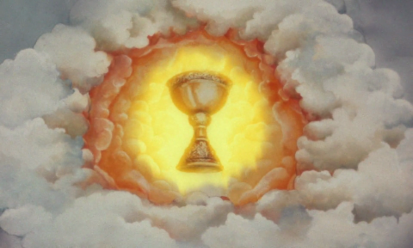
\includegraphics[height=4cm]{5-Quantum-orbits/Figures/figure5A.png}  \hspace{-1mm}\vspace{3mm}
\\ \hline
\end{tabular}
%\\ \hline
\end{tabular}
\vspace{4mm}

\caption[Schematic relationship between the SFA, CCSFA and ARM theories]{
Schematic depiction of the relationship between the Strong-Field Approximation (SFA), the Coulomb-corrected Strong-Field Approximation (CCSFA), and the Analytical $R$-Matrix (ARM) theory presented here. Ideally, we would like a first-principles derivation of a semiclassical theory building on the SFA and including Coulomb effects with the full Coulomb action: ARM theory approaches on the first-principles side and CCSFA uses a full Coulomb action, and both illuminate important aspects of the ideal theory.
}
\label{f5-holy-grail-table}
\end{figure}
\copyrightfootnote{
Holy Grail image in \reffig{f5-holy-grail-table} excerpted from \textit{Monty Python and the Holy Grail}, © National Film Trustee Company Ltd, 1974.
}




For now, though, we focus on the task at hand and examine the origin of the ARM trajectory \eqref{e5-laser-driven-trajectory}. The ARM gets its trajectory language, ultimately, from the same place that the usual SFA does: from its continuum wavefunctions. However, while the SFA takes its kinetic phase from the Volkov states
\begin{align}
\phantom{{}^\mathrm{EA}}
\braket{\vb{r}}{\vb{k}^{\mathrm{(V)}}(t)}
& = 
\frac{1}{(2\pi)^{3/2}}
e^{i\left(\vb{k}+\vba(t)\right)\cdot\vb{r}} 
e^{-\frac{i}{2} \int_T^t\left(\vb{k}+\vba(\tau)\right)^2\d\tau}
,
\phantom{e^{-i\int_T^t U_n(\rl(\tau;\vb{r},\vb{k},t),\tau)\d\tau}}
\backtag{e2-volkov-wavefunctions}
\end{align}
in ARM theory we introduce the Coulomb correction at this same wavefunction level where the trajectory language starts. Thus, ARM theory introduces the Coulomb phase $e^{-iW_C}=e^{-i\int_T^t V(\rl \d\tau}$ here, giving
\begin{align}
\braket{\vb{r}}{\vb{k}^{\mathrm{(EVA)}}(t)}
& = 
\frac{1}{(2\pi)^{3/2}}
e^{i\left(\vb{k}+\vba(t)\right)\cdot\vb{r}} 
e^{-\frac{i}{2} \int_T^t\left(\vb{k}+\vba(\tau)\right)^2\d\tau} 
e^{-i\int_T^t V(\rl(\tau;\vb{r},\vb{k},t),\tau)\d\tau},
\backtag{e2-eikonal-volkov-wavefunctions}
\end{align}
in terms of laser-driven trajectory
\begin{align}
\rl(\tau;\vb{r},\vb{k},t)
& \colonequals 
\vb{r}+\int_t^\tau \left(\vb{k}+\vba(\tau')\right)\d\tau'
.
\backtag{e2-trajectory}
\end{align}
Moreover, the form of this Coulomb phase $e^{-iW_C}$, and the trajectory it builds from, are not imposed on the wavefunction. Instead, the eikonal approximation \cite{eikonalVolkov_initial, eikonalVolkov_prelim} builds this phase from a WKB-like semiclassical series, which transforms the Schrödinger equation for $e^{-iS}$ into a Hamilton-Jacobi equation in $S$, whose solutions are precisely those built over the classical trajectories.

Implementing the eikonal-Volkov wavefunctions, on the other hand, does require additional machinery, because their perturbative treatment of the Coulomb field means that they cannot get too close to the ion and its Coulomb singularity. While this is not the only reason to introduce the $R$-matrix splitting of space into inner and outer regions (which is also essential for multi-electron effects), it does make the two methods ideally suited for each other. 

This means, then, that the eikonal Volkov states need to be matched at the $R$-matrix boundary using the procedure of chapter~\ref{chap:R-matrix}, and this connects them to a similar wavefunction on the other side -- the WKB tail of the ionizing orbital, which is also essentially of~the form
\begin{equation}
\psi_g(r) \propto C_\kappa e^{-i\int_{\tk}^{\tvr}U\left(\int_{\ts}^\tau \vbv(\tau')\d\tau' \right)\d\tau}.
\label{e5-ground-state-WKB-revisited}
\end{equation}
Here the `starting' time $\tk$ has some leeway, as changing $\tk$ only changes $\psi_g$ by a constant that can be absorbed into $\tk$, but the convenient choice is to set it to $\tk=\ts-i/\kappa^2$, which permits the WKB ground state \eqref{e5-ground-state-WKB-revisited} to coincide with the explicit expression \eqref{e2-wkb-explicit-expression} for the wavefunction. In trajectory language, this choice implies that the position at $\tk$ is roughly $1/\kappa$, the characteristic distance of the ionizing orbital. (This separation, while small, is nevertheless crucial, because for a Coulomb singularity the integral in~\eqref{e5-ground-state-WKB-revisited} diverges if taken for a trajectory that starts at the origin with $\tau$ up~to~$\ts$.)

The trajectory formulation for the ionizing state's WKB expression~\eqref{e5-ground-state-WKB-revisited} is the ultimate source of the initial condition for our final laser-driven trajectory \eqref{e5-laser-driven-trajectory}, since the eikonal-Volkov states \eqref{e2-eikonal-volkov-wavefunctions} are based on trajectories \eqref{e2-trajectory}, which have an arbitrary starting point set to the evaluation point $\vbr$; these starting points are averaged over the $R$-matrix boundary in the matching procedure and reduce to the WKB expression with a trajectory that starts at the origin at the ionization time~$\ts$.




%
%\subsection{Overview}
%Finally, and before we begin the technical analysis in earnest, it is worthwhile to comment on the lay of the land ahead. 
%
%
%
%
%





\section{Imaginary parts of the laser-driven trajectory}
Having examined the pedigree of our laser-driven trajectory, 
\begin{equation}
\rl(t) = \int_{\ts}^{t} \left[\vbp+\vba(\tau) \right] \: \d\tau
,
\backtag{e5-laser-driven-trajectory}
\end{equation}
we now turn to its structure. We focus specifically on a monochromatic field of the~form
\begin{equation}
\vba(t)=-\frac{F}{\omega}\un \sin(\omega t),
\backtag{e2-field-definition}
\end{equation}
though most of the results that follow will degrade smoothly if a reasonably slow envelope is introduced. In this chapter we will work in the laboratory frame, fixing the polarization direction to the $z$ axis.

Generally speaking, the laser-driven trajectory should be thought of as a general analytical function $\rl\colon \mathbb{C}\to \mathbb{C}^3$, and in principle it is defined for an arbitrary complex input, for which it reads
\begin{equation}
\rl(t)=(t-\ts)\vbp +\frac{F}{\omega^2}\uz \left(\cos(\omega t) - \cos(\omega \ts)\right)
,
\label{e5-explicit-rl-trajectory}
\end{equation}
with the cosine taking an arbitrary complex input as usual.

More specifically, though, we care about $\rl(t)$ because we need it to calculate the temporal integrals over the mean-field Coulomb potential as 
\begin{equation}
\int_\tk^T U_n(\rl(\tau)) \d\tau
\label{e5-coulomb-rl-integral}
\end{equation}
for the single-electron yield~\eqref{e2-ionization-yield-with-shape-factor}, and 
\begin{equation}
\int_{\ts}^T\! \Vnm{\rl(t)} e^{+i(E_n-E_m)t} \: \d t 
\end{equation}
over the correlation interaction potential for the correlation-driven yield~\eqref{e3-correlation-driven-yield-reprise-with-full-derivatives}. Both of these integrals start at (or near) the complex ionization time $\ts$, and they need to be taken until the detection time $T$, which should be large enough for the pulse to be over and for all ionization effects to have converged. 

Since the integrands in both cases are analytical, the path for these integrals can in principle be chosen arbitrarily, and the integral will always evaluate to the same value. However, for the sake of definiteness, as we saw in the Introduction with \reffig{f1-initial-contour}, the convention is generally to start at the complex ionization time $\ts = \tn + i\tauT$, integrate directly down to its real part $\tn=\Re(\ts)$ on the real axis, and then along the real axis until the detection time $T$, as shown in \reffig{f5-standard-time-contour}.


\begin{figure}[htb]
\centering
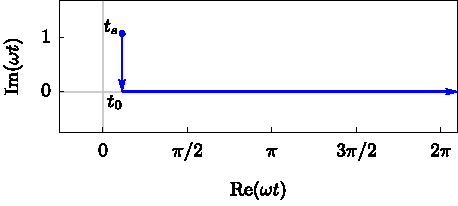
\includegraphics[scale=1]{5-Quantum-orbits/Figures/figure5B.pdf}
\caption[Standard integration path in the complex time plane, from the ionization time $t_s$ to its real part and then along the real axis]{Standard time contour used in complex-time theories of tunnelling ionization: down from the complex ionization time $\ts$ to its real part $\tn=\Re(\ts)$, and then along the real axis until the detection time $T$.}
\label{f5-standard-time-contour}
\end{figure}


This sort of contour is particularly useful conceptually, because it allows us to usefully separate a ``tunnelling'' part of the integration (the downward leg, where factors of the form $e^{-iEt}$ for complex $t$ impose the exponential unlikelihood of tunnelling processes) from a more classical propagation along the real axis where $e^{-iEt}$ factors are only phases as~usual and the electron is generally understood as having left the classically forbidden~region. As we shall see later, this standard contour can cause problems when we turn time into position using our laser-driven trajectory \eqref{e5-laser-driven-trajectory} and we run this through our potentials, but it is useful in many scenarios and it is certainly a reasonable default choice.


If we analyse this standard contour in terms of the trajectory $\rl(t)$, the most interesting part is the tunnelling segment -- the downwards leg from $\ts$ to $\tn$. Here, breaking the trajectory~\eqref{e5-explicit-rl-trajectory} down into explicit real and imaginary parts for an argument of the form $t=\tn+i\tau$, we can express it as
\begin{align}
\rl(\tn+i\tau)
= &
- i(\tauT-\tau)\vbpo
\nonumber \\ & \quad
+\frac{F}{\omega^2}\uz \left[\vphantom{\sum^n}
-\cos(\omega\tn)
\left( \vphantom{\sum}
\cosh(\omega\tauT)
-\cosh(\omega\tau)
\right)
\right. \nonumber \\ & \left. \vphantom{\sum^n} \qquad \qquad 
+i\left( 
-\omega(\tauT-\tau)\frac{\omega p_z}{F}
+
\sin(\omega\tn)(
\sinh(\omega\tauT)
-\sinh(\omega\tau)
)
\right)
\right]
.
\label{e5-explicit-rl-trajectory-re-im-parts}
\end{align}
%
Here we see that the combination $\cos(\omega t) = \cos(\omega \tn + i \omega\tau)$ will generally always produce a complex number whenever $\tn$, which is given by the explicit saddle-point equation
\begin{equation}
\omega \ts
=\omega\tn+i\omega\tauT
= \arcsin\left(
\frac{\omega}{F}\left(p_z + i \sqrt{\kappa_n^2+\pt^2}\right)
\right)
,
\backtag{e2-saddle-point-equation-final-solution}
\end{equation}
has a nonzero real part, which happens whenever $p_z$ is nonzero. Outside of the special case of $p_z=0$, then, the laser-driven trajectory $\rl(t)$ is always complex-valued once $t$ reaches the foot of the contour at the real axis, following the behaviour shown in \reffig{f5-imaginary-parts-of-position}.


\newcommand{\onemicronparsfield}{0.05} 
\newcommand{\onemicronparsomega}{0.0456} 
\newcommand{\onemicronparskappa}{1.07} 
\newcommand{\onemicronparswavelength}{1} 
\newcommand{\onemicronparsgamma}{0.98}
\begin{figure}[htb]
  \centering
  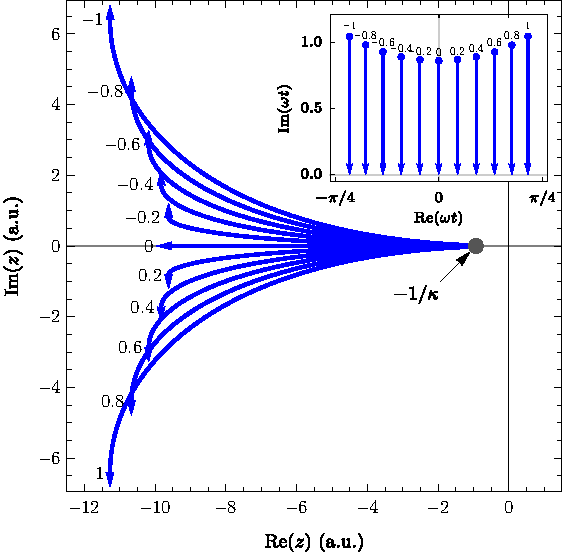
\includegraphics[scale=1]{5-Quantum-orbits/Figures/figure5C.pdf}
  \caption[
  Laser-driven trajectory $\zl(t)$ in the complex $z$ plane, over the ``tunnelling'' downwards leg of the standard time contour
  ]{
  The laser-driven trajectory $\rl(t)$ on the complex $z$ plane, corresponding to the ``tunnelling'' part of the standard contour where $t$ goes from the complex tunnelling time $\ts$ down to its real part $\tn$ on the real axis, with the time contour segments shown in the~inset.
  Here, and in the rest of this chapter unless otherwise stated, we set $F=\SI{\onemicronparsfield}{\au}$, $\omega=\SI{\onemicronparsomega}{\au}$ and $\kappa=\SI{\onemicronparskappa}{\au}$, corresponding to argon ionized by a $\SI{\onemicronparswavelength}{\micro m}$ field at $\SI{e14}{W/cm^2}$, with Keldysh parameter $\gamma=\onemicronparsgamma$.
  }
\label{f5-imaginary-parts-of-position}
\end{figure}


In addition to this, if there is any nonzero transverse momentum $\vbpo$ orthogonal to the polarization direction, then upon reaching the real axis the position on the transverse plane will be completely imaginary, at $-i\tauT\vbpo$, since here the electron has a real velocity and propagates through an imaginary time interval. 

In the longitudinal direction, on the other hand, in the special case that $p_z=0$ the electron has a completely imaginary velocity $v_z(\ts)=\sqrt{-2I_p}$, and it propagates over an imaginary time interval, so it accrues only real-valued changes in position, as it does in the quasi-static case described in the Introduction. For nonzero $p_z$, on the other hand, the velocity is only completely imaginary at the moment of tunnelling, but it acquires a nonzero real component as the electron crosses the classically forbidden region, and this results in a nonzero imaginary part that increases with $|p_z|$.

On the other hand, once the integration contour reaches the real axis, this imaginary part of $\rl(t)$ can be considered to be `frozen' as long as the time contour stays on the real axis, because the velocity $\vbp+\vba(t)$ is real-valued there so its integral can only accumulate real-valued changes. 

One approach to this is to take this as a marker that the imaginary part of the position is an artefact of the method, which is only valid as a construct for use in computations: it no longer plays a role in the dynamics of the trajectory,%
%
\footnote{%
However, it is worth pointing out that for a complex-valued trajectory under the action of the Coulomb potential this is no longer true, and the imaginary part will both change and affect the evolution of the real part. Thus, dismissing the dynamics of the imaginary part of the trajectory over the real time axis is equivalent to closing the door on extensions to the theory that include Coulomb-corrected trajectories.
}
and it only needs to be tracked as a calculational tool to compute the quantum Coulomb corrections, but one can argue that it has no physical significance. (Of course, this can be said about any given concept in a physical theory.) Even within that viewpoint, however, the imaginary part of the trajectory is operationally as relevant as the real part. Moreover, it is important to note that complex-valued trajectories are not confined to this method, and they are a rather general feature of quantum mechanics when it is pushed into trajectory language~\cite{goldfarb-tannor_bohmian-complex_2006, goldfarb-tannor_complex-trajectory-wkb_2008, schiff-tannor_path-integral-complex-trajectory_2011}. 

In addition, connecting back to our motivations for finding trajectory language in the first place, we set out to see if it is possible to derive a model, entirely within the TDSE and without adding in the Coulomb field by hand, that includes the trajectory language used by CTMC approaches. The ARM results then teach us that it is indeed possible, but that the TDSE-based trajectories come with a complex component, and that one ignores this at one's own peril. With this we turn, then, to the consequences of this imaginary part when it is included in the Coulomb interaction.











\section{Emergence of temporal branch cuts}
As we saw in chapter~\ref{chap:complex-space-potentials}, in general it is possible to calculate the correlation interaction potential $\Vnm{\rl(t)}$ when the argument $\vbr=\rl(t)$ is complex, but this needs to be confined to the safe region
\begin{equation}
\Re(\vbr^2)>0
\backtag{e4-re-r2-less-than-0}
\end{equation}
where the gaussian-based methods give reasonable answers and we can be reasonably sure that our models are correct, so we need to ensure that the laser-driven trajectory never leaves this region.

In addition to this, the mean-field potential $U_n(\vbr)$ also imposes requirements when it is applied to a complex argument. These requirements can be similar to those of the correlation interaction potential when $U_n(\vbr)$ is taken to be the mean field of a full molecular charge, but in this chapter we will focus on the bare basics of this potential and simply take it to be a Coulomb potential, which is in any case always present. This will be plenty to keep us busy, and most of the results generalize to a broader class of potentials.

The Coulomb potential is problematic because, when extended to its analytical continuation over complex positions, it requires a square root to remain analytical:
\begin{equation}
U(\vbr) = -\frac{1}{\sqrt{\vbr^2}}= -\frac{1}{\sqrt{x^2+y^2+z^2}}.
\label{e5-coulomb-potential}
\end{equation}
This means that the Coulomb potential goes from having an integrable singularity at the origin to having a branch cut along the ray $\vbr^2\in (-\infty,0]$; this is where the standard branch, as we defined it in \eqref{e4-square-root-definition}, resolves the ambiguity of whether to assign $\sqrt{-1}$ to $+i$ or $-i$ by having a discontinuous sign change of the imaginary part: numbers with a slightly positive imaginary part are assigned to the neighbourhood of $+i$, as $\sqrt{-1+i\varepsilon}\approx i+\varepsilon/2$, and numbers with a slightly negative imaginary part are assigned to the neighbourhood of $-i$, as $\sqrt{-1-i\varepsilon}\approx -i+\varepsilon/2$.



However, unlike our previous encounter with this branch cut in \eqref{e4-square-root-definition}, where all we needed was a definite integrand to calculate with, here the Coulomb cut has very deep consequences, because the Coulomb potential is now being directly integrated in a complex path integral. Indeed, if one integrates across the branch cut's discontinuity, the dependence on $t$ of the Coulomb integrand in \eqref{e5-coulomb-rl-integral} ceases to be analytic, and one loses the freedom that allowed the real contour of \eqref{e2-yield-after-saddle-point-approximation} to be deformed to pass through the saddle-point $\ts$ in the first place. In other words, all the work since the initial saddle-point approximation over the tunnelling time $\ts$ would become invalid.



\captionsetup[figure]{position=auto}

\begin{figure}[t!]
  \centering
  \captionsetup[figure]{position=b}
  \captionsetup[subfigure]{position=b}
  \subfloat{
    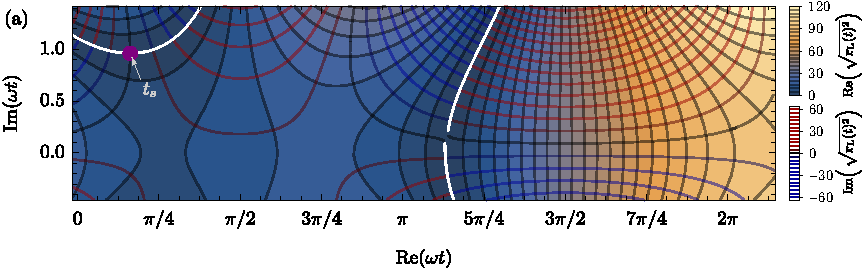
\includegraphics[scale=1]{5-Quantum-orbits/Figures/figure5Da.pdf}
    \label{f5-complex-position-contour-plot}
  }
  \\[-3mm]
  \subfloat{
    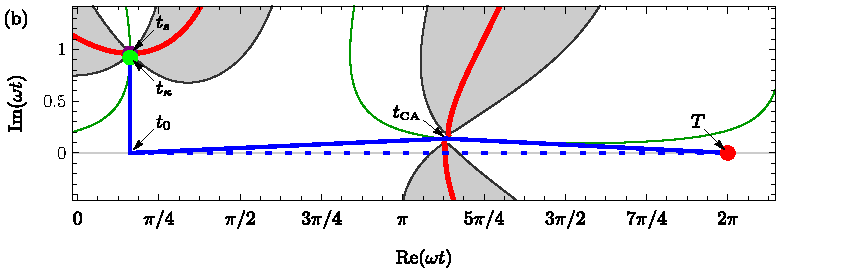
\includegraphics[scale=1]{5-Quantum-orbits/Figures/figure5Db.pdf}
    \label{f5-branch-cut-sketch}
  }
  \captionsetup{width=\textwidth}
  \caption[
  Riemann surface of $\sqrt{\rcl(t)^2}$ over the complex time plane, showing branch cuts that cross the standard integration path along the real axis
  ]{
  \protect\subref{f5-complex-position-contour-plot} Contour plot of the complex distance to the origin, $\sqrt{\rcl(t)^2}$, with the coloured background along the real part and the red, black and blue orthogonal lines representing, respectively, positive, zero and negative imaginary parts. The white lines are branch cuts where the real part is zero and the imaginary part discontinuously changes sign.
  In \protect\subref{f5-branch-cut-sketch} we show a simplification of this picture, with the red lines showing the branch cuts, and the thin green lines the positive real axis of $\vbr^2$. The shaded regions indicate the complex times for which $\Re(\rcl(t)^2)$ is negative, which are undesirable when using gaussian and numerically-obtained ionic potentials, as they would be unphysical there.
  The momentum displayed, $\vbp=(\figurefiveDpo,0,\figurefiveDpp)$, is such that the standard contour (integrating down to the real part $\tn$ of the saddle point $\ts$ and then along the real axis, shown dotted in \protect\subref{f5-branch-cut-sketch}) crosses a branch cut. Instead, one should choose a contour which passes through a time between the branch cuts, which we label $\tca$ and explore in detail in Sec.~\ref{sec:times-of-closest-approach}.
  }
  \label{f5-complex-position-branch-cuts}
\end{figure}


To be somewhat more definite, the branch cut occurs when $\vbr^2$ is real and negative, and~since we can write it as
\begin{equation}
\vbr^2=\Re(\vbr)^2-\Im(\vbr)^2+2i\Re(\vbr)\cdot\Im(\vbr),
\label{e5-r2-parts-breakdown}
\end{equation}
this means that the branch cut requires $\Re(\vbr)$ to be smaller than $\Im(\vbr)$ and occurs when the two are perpendicular. This is relatively hard to picture geometrically, but fortunately there are simpler tools to analyse this. In particular, we only need to consider the entire potential as a single, function of time,
\begin{equation}
U(\rl(t)) = -\frac{1}{\sqrt{\rl(t)^2}},
\label{e5-coulomb-potential-at-the-trajectory}
\end{equation}
a single analytical function of the complex-valued variable $t$, and in this perspective the branch cuts in $U$ are imprinted on the complex time plane via the conformal mapping $t\mapsto \rl(t)^2$. To see this, we show in \reffig{f5-complex-position-contour-plot} an example of the Coulomb potential's behaviour, as a complex conformal map of the function $\sqrt{\rl(t)^2}$ (which has the same branch-cut structure as $U$, but omits the latter's singularities). 




The essential features of this function are the branch cuts, which are shown in white, with a discontinuous sign change in the imaginary part of $\sqrt{\rl(t)^2}$. Unfortunately, the full conformal map can obscure some information, like the position of the real axis, so we show in \ref{f5-branch-cut-sketch} a sketch with the essentials of this function, with the branch cuts shown in red. Here it is important to note that the standard integration contour of \reffig{f5-standard-time-contour} -- straight down from the complex ionization time $\ts$, and then along the real axis, shown dotted in \reffig{f5-branch-cut-sketch} -- can indeed cross the branch cuts when the electron returns near the ion.



\begin{figure}[t!]
  \centering
  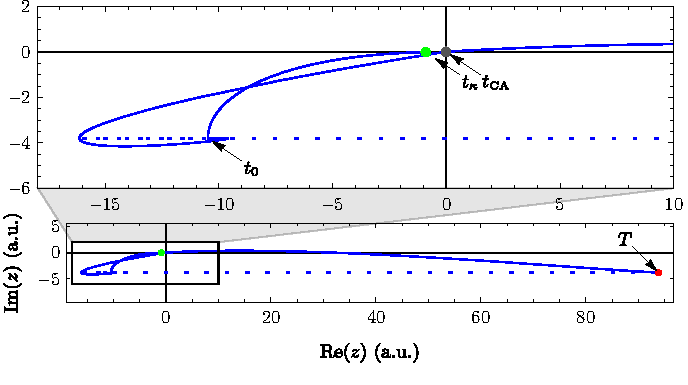
\includegraphics[scale=1]{5-Quantum-orbits/Figures/figure5E.pdf}
  \caption[
  Complex-space trajectory $\zcl(t)$ corresponding to an integration path altered to avoid a Coulomb branch cut
  ]{
  Trajectories in the complex $z$ plane corresponding to the contours shown in \reffig{f5-branch-cut-sketch}. The trajectory starts at $z=-1/\kappa$ at time $\tk$, and departs somewhat from the real position axis as the time goes down to the real axis at $\tn$, as shown in \reffig{f5-imaginary-parts-of-position}. Along the real axis, on the standard contour shown dashed, the electron goes to large negative $\Re(z)$ before turning around towards the core. It then reaches the ion with a large imaginary part, which causes a discontinuous jump in the square root of~\eqref{e5-coulomb-potential}. Deforming the contours to avoid the branch cuts, shown in the solid line, minimizes the imaginary part of $z$ at the moment of recollision; it is then slowly regained before detection at a large real time $T$. The closest approach time $\tca$ marks the minimum value of $\Re(\rcl(t)^2)$ once the $x$ coordinate is taken into account; there $\zcl$ is small but nonzero.
  }
  \label{f5-complex-z-curved-contours}
\end{figure}



This means that to preserve the analyticity of the Coulomb integral~\eqref{e5-coulomb-rl-integral} one must deform the integration contour away from the real axis until the integrand is continuous and analytic throughout the integration path. This will correspondingly change the way the complex position $\rl(t)$ moves through complex space, and the effect turns out to be one of \textit{minimizing} the imaginary part of the position at the time of recollision, when $\Re(\vbr)$ is small, so that the branch cut from \eqref{e5-r2-parts-breakdown} is then avoided. We show in \reffig{f5-complex-z-curved-contours} the corresponding change in the path of $\zl(t)=\uz\cdot\rl(t)$ through the complex plane, as the time $t$ traces out the original, standard time integration contour, shown dashed, and the new, modified contour that avoids the branch cuts, shown as a solid line.


The relationship between the chosen temporal contour and the corresponding trajectory in complex position space, particularly along $z$, is in general rather complicated and it is a hard quantity to visualize. Similarly, the final momentum $\vbp$ has a strong effect on the dependence of the potential $U(\rl(t))$ as a function of time, sometimes very sensitively. To complicate matters further, these variables are all intertwined, with the changes in the momentum affecting the structure of the branch cuts, and therefore the possible paths that the time integration contour can take.



The intertwining of these variables makes the analysis of these situations relatively awkward, and to help disentangle these effects the author has written a software package, the Quantum Orbits Dynamic Dashboard software available as \citer{QuODD}, that enables the user to visualize the effects on the complex-space trajectory of different modifications on the complex-time integration path and of changes in the momentum or the ionization time~$\ts$. We display, in \reffig{f5-quodd-screenshot}, a screen capture of this software, along with its major features. Among other features, the package allows the wide variety of different integration paths to be visualized, by showing in real time the effects of such modifications on the complex-space trajectories as well as the Coulomb integrand.




\begin{figure}[htb]
  \centering
  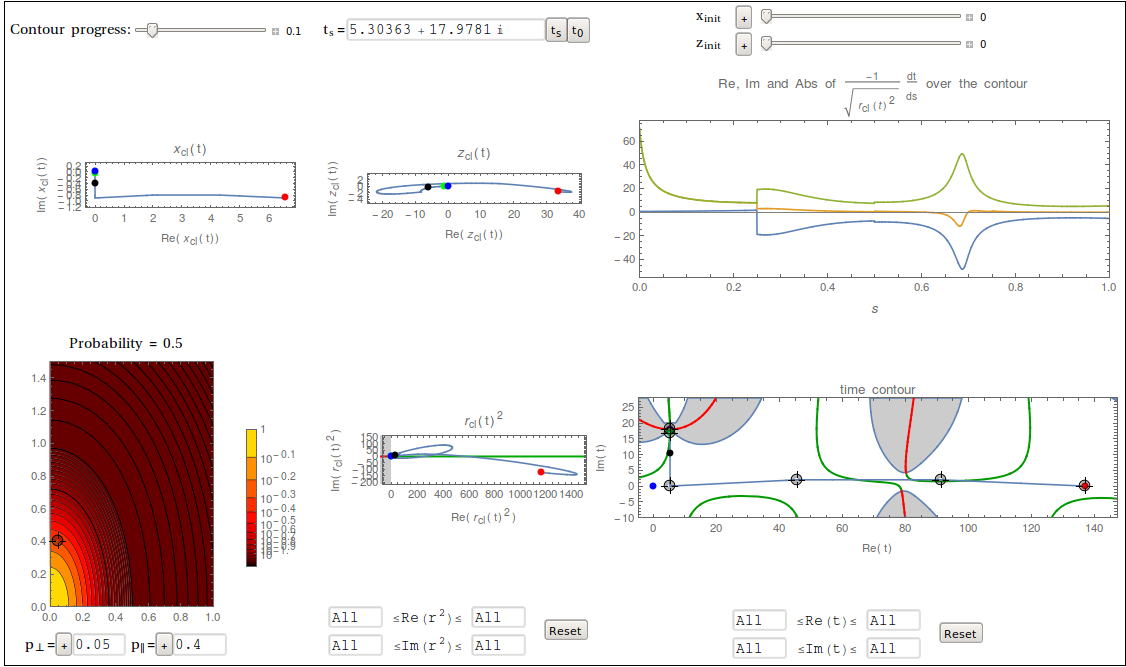
\includegraphics[width=\textwidth]{5-Quantum-orbits/Figures/figure5M.png}
  \captionsetup{width=\textwidth}
  \caption[
  Screenshot of the Quantum Orbits Dynamic Dashboard software
  ]{
  Screenshot of the Quantum Orbits Dynamic Dashboard software from \citer{QuODD}, an open-sourced Mathematica package. The main panels show, on the top row, the $x$ and $z$ coordinates of the laser-driven trajectory, together with the Coulomb integrand, for an integration path over complex time shown at bottom right over a branch cut sketch similar to \reffig{f5-branch-cut-sketch}. (Similarly, the bottom-centre panel shows a complex-plane plot of $\rl(t)^2$.) This integration path, along with the asymptotic momentum $\vbp$, shown at bottom left, and the ionization time $\ts$, can be dynamically modified, with the effects of these modifications on the trajectory and the branch-cut layout tracked in real time.
  }
\label{f5-quodd-screenshot}
\end{figure}






The presence of these Coulomb branch cuts in the complex plane has appeared in the literature occasionally~\cite{popruzhenko_branch-cuts_2014}, but only rarely has it been necessary to shift the integration path away from the sandard contour~\cite{ popruzhenko_branch-cuts_2014, Milosevic_scattering_large}. However, as we have shown, once the electron trajectory is obtained from the ground state through the ARM boundary matching, instead of having an initial condition imposed externally, they become inevitable.

In the rest of this chapter we will show how to handle these branch cuts, by providing an algorithm to programmatically choose a correct integration path, and we will explore the rich geometry unearthed by its key constituents, the times of closest approach to the ion. Later on, in chapter~\ref{chap:LES-NZES}, we will use this method to relate our calculations to experimental features photoelectron spectra. 

A more recent analysis~\cite{keil_branch-cuts_2016}, focusing on ATI spectra at the crossover between direct and rescattered electrons at $2U_p$, also confirms our findings, showing that the photoelectron spectrum there can only be analyzed correctly if a complex tunnel exit is taken into account, with the attendant branch cuts similarly forcing changes in the integration path, which can again be handled well with the method that we provide below.












\section{Times of closest approach}
\label{sec:times-of-closest-approach}
We see, then, that it is possible for branch cuts of the Coulomb potential to cross the real axis, thereby precluding the use of the standard integration contour of \reffig{f5-standard-time-contour} for the Coulomb integral in \eqref{e5-coulomb-rl-integral}, but that it is still perfectly possible to choose temporal integration paths which remain valid by avoiding the branch cuts, passing through the ``slalom gate'' left by the branch cuts of $U(\rl(t))$ as in \reffig{f5-complex-position-contour-plot}.

This can easily be done by hand, by shifting the contour appropriately, if only a single or a few momenta need to be handled, but it is certainly infeasible if one needs to compute a photoelectron spectrum, sampling a large number of different momenta. What is needed, then, is a computational approach: we require a programmatic way to automatically choose the correct integration contour for any given momentum.

The key to obtaining this approach is to examine in detail the space between the two branch cuts, as shown in \reffig{f5-tCA-zoom}. Each branch cut is a contour of constant $\Re(\sqrt{\rl(t)^2})$, which measn that the neighbouring contours must closely follow its direction, and circle around it when it terminates at the branch point. 

\begin{figure}[htb]
  \centering
  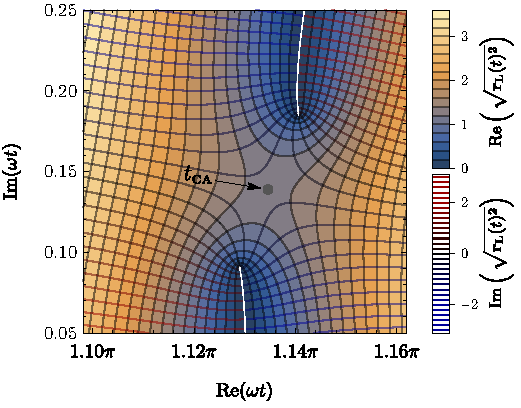
\includegraphics[scale=1]{5-Quantum-orbits/Figures/figure5F.pdf}
  \caption[
  Closer view of the `slalom gate' between two paired Coulomb branch cuts
  ]{
  Closer view of the region between the branch cuts in \reffig{f5-complex-position-contour-plot}. The space between any two branch cuts always contains a saddle point $\tca$, as this is the only way to join the curvatures of the contours next to each branch cut. For contours that pass through it, the saddle point marks the minimum of $\Re\left(\sqrt{\rl(t)^2}\right)$. For valid contours that do not pass through $\tca$, this minimum will be smaller.
  }
  \label{f5-tCA-zoom}
\end{figure}

In the slalom-gate configuration of \reffig{f5-complex-position-contour-plot}, the branch cuts come in pairs that face each other, and they must therefore have two sets of curved  contours at $\Re(\sqrt{\rl(t)^2})=\mathrm{const.}$, facing each other, that must somehow meet in the middle; the only way for this to happen is for there to be a saddle point between the branch cuts. This saddle point is the crucial object which enables the programmatic choice of a contour that avoids the branch cuts, since the saddle point is at the ideal location in between the two cuts. Moreover, the saddle point has a deep physical and geometrical significance, which we will now explore.

To begin with, it is clear from \reffig{f5-tCA-zoom} that if we track the real part of the complex distance to the origin, $\Re(\sqrt{\rl(t)^2})$, over any integration path which crosses the complex~$t$ plane from left to right of the region shown in the figure, $\Re(\sqrt{\rl(t)^2})$ must always decrease, reach a minimum, and then increase again. For some paths -- the ones that cross the branch cuts -- the minimum value of $\Re(\sqrt{\rl(t)^2})$ is zero, but these are forbidden as integration paths. From within the allowed paths, the minimum is shallowest when the path passes through our saddle point.

For this reason, then, we call the saddle point the time of closest approach, and we label it $\tca$. To be precise, then, an integration path that passes through $t=\tca$ maximizes the minimum value of the real part of the distance to the origin, $\Re(\sqrt{\rl(t)^2})$; in addition, it can also be seen to maximize the minimum value of the absolute value, $\left|\sqrt{\rl(t)^2}\right|$, as well. Intuitively, it permits the furthest possible approach to the ion, keeping the origin at arm's length as much as possible.

Similarly, when calculating the Coulomb potential along such a contour, this choice of path minimizes the maximum value of the real part and absolute value of $1/\sqrt{\rl(t)^2}$ (for valid contours which do not cross the branch cuts), so that the Coulomb interaction is kept as bounded as possible throughout the integration. As long as the potential $U(\rl(t))$ stays continuous and analytic, this is not essential (as the integral in \eqref{e5-coulomb-rl-integral} will not change) but passing through $\tca$ means reaching a smallish value through adding smallish quantities, rather than through cancellations between bigger ones. In addition, this choice optimizes the applicability of the approximations that led to \eqref{e5-coulomb-rl-integral}, and it admits the clearest physical interpretation by keeping the imaginary part of the position within the tightest relevant bound possible at the points where this is necessary.

To actually find these saddle points, one simply looks for the zeroes of the time derivative of $\sqrt{\rl(t)^2}$. More simply, though, this can be reduced to the zeroes of $\tfrac{\d}{\d t}\left[\rcl(t)^2\right]$, since they coincide with the zeroes of the square root, so the main criterion is simply
\begin{equation}
\rl(\tca)\cdot\vbv(\tca)=0.
\label{e5-tca-equation}
\end{equation}
This equation is deceptively simple, and one must remember that the left-hand side is a complex-valued function of time through Eq.~\eqref{e5-laser-driven-trajectory}. Nevertheless, it has a compelling physical interpretation, for if a classical electron passes near the nucleus then it is closest to the origin when its velocity and its position vector are orthogonal. This then lends further support to our choice of name for the $\tca$.

In this spirit, then, it is worthwhile to investigate the classical solutions of \eqref{e5-tca-equation} before exploring the solutions in the complex quantum domain. As we shall see, both domains exhibit rich geometrical structures which are closely related to one another. After exploring the geometrical implications in both contexts, we shall use this knowledge to automatically generate correct integration paths for any momentum.







\subsection{Classical solutions}
\label{sec:classical-tcas}

In this context, we can introduce a classical equivalent of our theory by simply taking the real part of our working laser-driven trajectory, as
\begin{equation}
\rcl(t) = \Re\left(\int_{\ts}^{t} \vbp+\vba(\tau) \: \d\tau\right)
,
\label{e5-classical-trajectory}
\end{equation}
and only considering real times. This simplified model is widely used as the classical version of tunnelling, since it is capable of encapsulating much of the tunnelling dynamics in terms of the tunnel exit position $\rl(\tn)$ after integration over the downward leg of the standard contour, while still having a real-valued trajectory that lends itself to further manipulation, as
\begin{equation}
\rcl(t) =  \Re\left(\rl(\tn)\right) + \int_{\tn}^{t} \left[ \vbp+\vba(\tau) \right] \: \d\tau
.
\label{e5-explicit-classical-trajectory}
\end{equation}
Indeed, this real-valued trajectory is the starting point for classical-trajectory based theories like CCFSA or Classical Trajectory Monte Carlo methods, which keep the initial term $\Re(\rl(\tn))$, and then modify the subsequent continuum dynamics.

Within this model, then, the closest-approach points obey the real part of our initial equation \eqref{e5-tca-equation}, 
\begin{equation}
\Re\left[\rl(\tcacl)\cdot\vbv(\tcacl)\right]
=
\rcl(\tcacl)\cdot\vbv(\tcacl)=0
,
\label{e5-tca-classical-equation}
\end{equation}
taken over real times. Unfortunately, this equation -- like the full quantum equation~\eqref{e5-tca-equation}~-- has more solutions than the closest-approach times we want, and these are not always distinguishable from the desired $\tca$. Specifically, the turning points of the classical trajectory, away from the core, are also solutions of \eqref{e5-tca-classical-equation}, since they are also extrema of~$\vbr^2$. On the quantum side, the surface of \reffig{f5-complex-position-contour-plot} also contains saddle points at $\omega t\approx \pi/4$ and $\omega t \approx 3\pi/4$, which correspond to the turning points shown in \reffig{f5-complex-z-curved-contours} to the right and left of the position at $\tn$, respectively.  This means that, to be able to use the closest-approach times as an effective tool to avoid the branch cuts, we will need to distinguish the crucial mid-gate $\tca$ points from the other solutions, and in general this will not be trivial.

In certain cases, though, this is easy, such as for the on-axis case when $\pt=0$, where \eqref{e5-tca-classical-equation} reads
\begin{equation}
\Re\left(\zl(\tcacl)\right)v_z(\tcacl)=0
,
\label{e5-tca-classical-equation-on-axis}
\end{equation}
with solutions that separate cleanly into turning points, for which $v_z(\tcacl)=0$, and closest approaches which degenerate to nucleus flybys at $\zcl(\tcacl)=0$, as shown in \reffig{f5-classical-tca-on-axis}. In this case, the turning points can additionally be classified as minima and maxima of $\rcl(t)^2$, shown respectively in green and red in \reffig{f5-classical-tca-on-axis}, by evaluating the sign of $\tfrac{\d^2}{\d t^2}\rcl(t)^2$. At nonzero $\pt$, it is the collisions that will turn into useful closest-approach times.



\begin{figure}[t!h]
\centering
%\begin{tabular}{c}
%\raisebox{25mm}{\subfloat[]{\makebox[5mm][0mm]{} }}\hspace{-11mm} &
%\addtocounter{subfigure}{-1}
  \subfloat{
    \includegraphics[scale=1]{5-Quantum-orbits/Figures/figure5Ga.pdf}
    \label{f5-classical-tca-on-axis}
  }
  \\
%\raisebox{40mm}{\subfloat[]{\makebox[5mm][0mm]{} }}\hspace{-4mm} &
%\addtocounter{subfigure}{-1}
  \subfloat{
    \includegraphics[scale=1]{5-Quantum-orbits/Figures/figure5Gb.pdf}
    \label{f5-classical-tca-surface}
  }
%\end{tabular}
  \caption[
  Classical closest-approach times, both on-axis at $p_\perp=0$ and as a cusped surface in $\{(\vbp,t)\}$ space
  ]{
  The classical closest-approach times with $p_\perp=0$, satisfying \eqref{e5-tca-classical-equation-on-axis}, separate into two curves  \protect\subref{f5-classical-tca-on-axis}: turning points with $v_z=0$, and collisions with $\zcl=0$, with their intersections representing soft recollisions. At the points marked \texttt{a}, \texttt{b} and \texttt{c} the different roots merge and disappear, with the corresponding trajectories displayed in \reffig{f5-sample-trajectories}.
  For nonzero $p_\perp$, the solutions of the vector equation \eqref{e5-tca-classical-equation} form a single coherent surface \protect\subref{f5-classical-tca-surface} with a sequence of bounded lobes which connect at the soft recollisions, where the surface is locally a cone.
  Local minima and maxima of $\rcl(t)^2$ are shown respectively in green and red in both panels. At the boundary between the two, a maximum and minimum meet, merge and disappear, as shown in the trajectory of \reffig{f5-sample-trajectories-d}; the point then leaves the surface.
  The side  and bottom panels show the projections of the surface on $p_z$ and $p_x$ respectively. 
  An interactive 3D version of this figure is available as Fig.~\href{https://electrondynamicsincomplextimeandspace.github.io/\#figure-s1}{S1} in the Supplementary Information \cite{SupplementaryInformation}.
 }
  \label{f5-classical-tca-plots}
\end{figure}

One of the most interesting features of \reffig{f5-classical-tca-on-axis} is the intersections of the two curves shown, the points at which $\zcl(t)=0$ as well as $v_z(t)=0$, which we will term \textit{soft recollisions} for obvious reasons. In chapter~\ref{chap:LES-NZES} we will link these soft recollisions to interesting physical effects and features on the photoelectron spectra, but for now we will focus on their pivotal role within the geometry of the times of closest approach. Even in the restricted geometry of \reffig{f5-classical-tca-on-axis} they are already crucial, since at these points the number of available roots as $p_z$ is swept across them changes from one to three, as an `inward' turning point turns into an `outward' turning point flanked by two closest-approach points. The classical trajectory shows exactly this behaviour, as shown in \reffig{f5-sample-trajectories}, with this change in $p_z$.

The roots of \eqref{e5-tca-classical-equation-on-axis} can also merge at the extremes of the sinusoidal turning-point curve of \reffig{f5-classical-tca-on-axis}. At these points, the longitudinal momentum becomes greater than the oscillation amplitude $F/\omega$, and the velocity $v_z(t)=p_z - \frac{F}{\omega}\sin(\omega t)$ no longer changes sign. The resulting behaviour of the trajectories is shown in Figs.~\reffig{f5-sample-trajectories-b} and \subref{f5-sample-trajectories-c}, and resembles pulling a winding string until the turns are straight.


\begin{figure}[t]
\begin{center}
  \subfloat{\label{f5-sample-trajectories-a}}%
  \subfloat{\label{f5-sample-trajectories-b}}%
  \subfloat{\label{f5-sample-trajectories-c}}
  \subfloat{\label{f5-sample-trajectories-d}}%
  \includegraphics[scale=1]{5-Quantum-orbits/Figures/figure5H.pdf}
\end{center}   
  \caption[
  Classical trajectories near the critical points of the closest-approach surface
  ]{
  Classical trajectories from near the critical points marked \texttt{a}-\texttt{d} in \reffig{f5-classical-tca-plots}, where the closest-approach roots of \eqref{e5-tca-classical-equation} can merge and disappear, indexed by their reduced momentum $(\omega p_x/F,\omega p_z/F)$. The dots show closest-approach points, which satisfy \eqref{e5-tca-classical-equation} and for which the tangent to the trajectory is orthogonal to the radius vector.
  In the neighbourhood of a soft recollision, \protect\subref{f5-sample-trajectories-a}, an inward turning point turns into an outward turning point flanked by closest-approach points as the momentum increases.
  In \protect\subref{f5-sample-trajectories-b} and \protect\subref{f5-sample-trajectories-c} two turning points, a maximum and a minimum of $\rcl(t)^2$, merge and disappear as $p_z$ goes past the oscillation amplitude $F/\omega$, either in the positive \protect\subref{f5-sample-trajectories-b} or negative \protect\subref{f5-sample-trajectories-c} direction, so $v_z$ no longer changes sign and no turning points occur.
  Similarly, as the transverse momentum $p_x$ increases in \protect\subref{f5-sample-trajectories-d} the $x$ component of the velocity becomes too great for the tangent to be orthogonal to the radius vector; at that point a maximum and minimum of $\rcl(t)^2$ merge and disappear, leaving $\rcl(t)^2$ to grow monotonically.
  }
  \label{f5-sample-trajectories}
\end{figure}


The closest-approach solutions of \eqref{e5-tca-classical-equation} become more interesting when one allows a nonzero transverse momentum $\pt=p_x$. Here the solutions form a single coherent surface, shown in \ref{f5-classical-tca-surface}, that consists of a number of bounded lobes joined together at the soft recollisions, which locally look like cones. Thus, it is possible to continuously connect any two roots of~\eqref{e5-tca-classical-equation} via a path on the surface: the inward turning points and the recollisions, shown as separate green curves in \reffig{f5-classical-tca-on-axis}, can always be smoothly connected via the $p_x\neq 0$ component of the surface. This, in turn, precludes the existence of a simple criterion to distinguish one from the other in the general case.







\begin{figure}[t!]
  \centering
  \includegraphics[scale=1]{5-Quantum-orbits/Figures/figure5I.pdf}
  \caption[
  Quantum solutions of the closest-approach equation
  ]{
  The quantum solutions of the closest-approach equation \eqref{e5-tca-equation} form multiple surfaces which wrap around the classical solutions of \reffig{f5-classical-tca-surface}, closely following the lobes, where the latter exist, and departing at the edges to form pairs of parallel surfaces with imaginary parts of opposite sign. 
  Black dots represent largely real solutions, with red (blue) dots representing solutions with positive (negative) imaginary part.
  An interactive 3D version of this figure is available as Fig.~\href{https://electrondynamicsincomplextimeandspace.github.io/\#figure-s2}{S2} in the Supplementary Information~\cite{SupplementaryInformation}.
 }
  \label{f5-quantum-tca-surface}
\end{figure}


On the other hand, the outward turning points can still be distinguished, as they are the local maxima of $\rcl(t)^2$ and have a different sign of the second derivative $\tfrac{\d^2}{\d t^2}\rcl(t)^2$. These maxima are shown in red in Figs.~\ref{f5-classical-tca-on-axis} and~\subref{f5-classical-tca-surface}, and they form the ``left-facing'' side of the surface in \reffig{f5-classical-tca-surface}. Thus, any horizontal line of constant momentum must enter the surface through a maximum of $\rcl(t)^2$ (red) and leave it through a minimum (green), because the minima and maxima must alternate for any given trajectory. This means that the red (maximum) side of the surface points towards negative $t$, and the green (minimum) side points towards positive $t$. At the boundary between these two parts of the surface, a maximum and a minimum merge and disappear, and the trajectory will then behave as shown in Figs.~\ref{f5-sample-trajectories-b}, \subref{f5-sample-trajectories-c}, or \subref{f5-sample-trajectories-d}, depending on which direction the boundary is approached (i.e. towards positive $p_z$, negative $p_z$, or increasing $|p_x|$, respectively). Horizontal lines of constant momentum will be tangent to the surface at this boundary, and the corresponding trajectory will have a double root of~\eqref{e5-tca-classical-equation}.



\subsection{Quantum solutions}

The quantum solutions have a richer geometry, with an additional dimension -- imaginary time -- to be occupied. The immediate effect of this is to increase the number of available solutions: while in the classical case two real solutions of~\eqref{e5-tca-classical-equation} can merge and disappear, as they do in the points marked \texttt{b} and \texttt{c} in \reffig{f5-classical-tca-on-axis}, in the quantum case the complex solutions of \eqref{e5-tca-equation} are not lost, but will instead move into imaginary time and remain present.



In general, the quantum solutions will be close to the classical ones when the latter exist. As one approaches the end of a lobe on the classical solution surface of \reffig{f5-classical-tca-surface}, however, the quantum solutions approach each other close to the real axis and then diverge into positive and negative imaginary time, keeping a relatively constant real part. If one then projects this to real times, the result is a pair of surfaces which closely follow the red and green parts of the classical surface, and then diverge into roughly parallel planes as they reach the end of each lobe. We show this behaviour in \reffig{f5-quantum-tca-surface}.


The first few closest-approach solutions are relatively easy to handle, and depend smoothly on the momentum. This includes the first minimum and maximum of $\rl(t)^2$, like the ones in \reffig{f5-complex-position-contour-plot}, the birth time $\ts$ itself, and a conjugate solution with negative imaginary part which should be ignored. These solutions occupy specific regions of the complex $t$ plane, as shown in \reffig{f5-complex-tca-plane-structures}, and they can be identified consistently. Moreover, these solutions exhibit close approaches at $\omega t\approx \pi/2$ and $\omega t \approx 3\pi/2$, which are the quantum counterpart of the classical maximum-minimum mergers shown in Figs.~\ref{f5-sample-trajectories-b} and~\subref{f5-sample-trajectories-c}. These are evident in \reffig{f5-complex-tca-plane-structures} as the converging surfaces at those times, and they are of relatively limited interest.



\begin{figure}[t!]
  \centering
  \begin{tabular}{c}
  \subfloat{
    \includegraphics[scale=1]{5-Quantum-orbits/Figures/figure5Ja.pdf}
    \label{f5-tca-grid-patterns}
  }
  \\[-3mm]
  \begin{tabular}{cc}
  \subfloat{
    \includegraphics[scale=1]{5-Quantum-orbits/Figures/figure5Jb.pdf}
    \label{f5-momentum-semicircle}
  }
  &
  \subfloat{
    \includegraphics[scale=1]{5-Quantum-orbits/Figures/figure5Jc.pdf}
    \label{f5-tca-mixing-paths}
  }
  \end{tabular}
  \end{tabular}
  \caption[
  Quantum closest-approach times on the complex time plane
  ]{
  The quantum closest-approach times, which satisfy \eqref{e5-tca-equation}, on the complex time plane. In \protect\subref{f5-tca-grid-patterns} we show the closest approach times corresponding to a grid in momentum space (shown inset). These are generally grid-like in the time plane, though after $\omega t=3\pi/2$ some solutions lie close to the real axis and cannot be discerned in this view.
  At the cusps of Figs.~\ref{f5-classical-tca-surface} and \ref{f5-quantum-tca-surface}, which correspond to soft recollisions, the regular grid-like behaviour breaks and the solutions can no longer be uniquely tagged. 
  This can be seen by following the semicircular path in momentum space shown in \protect\subref{f5-momentum-semicircle}, for which there are three solutions in the gray rectangle of \protect\subref{f5-tca-grid-patterns}, shown in detail in \protect\subref{f5-tca-mixing-paths}. Going once around the semicircle moves the $\tca$ along the bow-shaped curves and, upon returning to the initial point, permutes them cyclically.
  In particular, this path contains an avoided collision between the points marked 2 and 3, and a three-way avoided collision between points 9 and 10. This three-way interaction marks the soft recollision itself.
  An interactive 3D version of this figure, with considerable additional detail, is available as Figs.~\href{https://electrondynamicsincomplextimeandspace.github.io/\#figure-s3}{S3} and~\href{https://electrondynamicsincomplextimeandspace.github.io/\#figure-s4}{S4} in the Supplementary Information \cite{SupplementaryInformation}.
 }
  \label{f5-complex-tca-plane-structures}
\end{figure}


%\begin{figure}
%\caption{hello, this is a \href{http://google.com\#hello}{test}}
%\end{figure}



The most important $\tca$ close approaches occur at and near the soft recollisions, shown inside the gray rectangle of \reffig{f5-tca-grid-patterns} and in \reffig{f5-tca-mixing-paths}, with a complicated momentum dependence which we explore below. In the quantum domain, soft recollisions again represent interactions between three different closest-approach roots. Unlike the classical domain, however, the roots do not merge; instead, two of them move into imaginary time after a three-way avoided collision, shown in \reffig{f5-tca-mixing-paths} between the points marked 9 and~10. The proximity between the multiple saddle points mirrors the increased time the electron spends near the ion in the neighbourhood of a soft recollision.

More interestingly, this three-way collision marks a crucial topological change in the configuration of the branch cuts associated with the recollision, as shown in \reffig{f5-branch-cut-topology-change}. Each of the outer saddle points, $\tcasup{\,(1)}$ and $\tcasup{\,(3)}$, has a pair of branch cuts associated with it, in the same `slalom gate' configuration as in \reffig{f5-tCA-zoom}, and these go off into imaginary time. However, the way in which they do so changes as the longitudinal momentum $p_z$ passes the momentum $\pzsr$ of the soft recollision.


For $p_z$ below $\pzsr$, as in \reffig{f5-branch-cut-topology-open}, the branch cuts loop back to imaginary time without crossing the real time axis. As with the low-momentum trajectory of \reffig{f5-sample-trajectories-a}, the trajectory does not quite reach the collision, and the associated branch cuts do not force a change of contour. At $p_z=\pzsr$, however, the branch cuts touch and reconnect, and for $p_z>\pzsr$ the topology changes to the one shown in \reffig{f5-branch-cut-topology-closed}. Here the trajectory does pass the core, and the associated branch cuts do cross the real axis, forcing the integration contour to change and pass through the gates.


This process has profound implications for the ionization amplitude, because these drastic changes in the integrand occur precisely when it is largest. Thus, choosing the wrong contour in this region accounts for the largest contributions to the integrand, with a correspondingly large effect on the integral. More surprisingly, once the contour is forced to pass through the `gate' $\tca$s, for $p_z$ just above $\pzsr$, their contributions have the effect of suppressing the ionization amplitude there. We will see how this works in more detail in chapter~\ref{chap:LES-NZES}.


We now turn to the momentum dependence of the closest-approach times near the soft recollision, which again presents interesting topological features. The main problem is illustrated in Figs.~\ref{f5-momentum-semicircle} and \subref{f5-tca-mixing-paths}: the different solutions of \eqref{e5-tca-equation} mix, and there is no longer any way to distinguish them from each other, as there was in the classical case. More concretely, traversing a closed loop in momentum space, like the semicircle shown in \reffig{f5-momentum-semicircle}, will move the roots around in such a way that when one returns to the initial point the overall configuration is the same, but the saddle points have been permuted cyclically.

Topologically, this means that the surface defined by \eqref{e5-tca-equation} (a two-dimensional surface in a four-dimensional space) does not separate into distinct components; instead, the surface has a single connected component after $\omega t=3\pi/2$. On the other hand, the surface itself remains singly connected. 
%
%Both of these behaviours are explored in Figs.~S3 and S4 in the Supplementary Information~\cite{SupplementaryInformation}.


This mixing behaviour is unusual in the quantum orbit formalism, where the norm is for rather elaborate indexing schemes to be possible \cite{Becker_rescattering, milosevic_ISFA-standard_2007}, partly because there is usually a single free parameter that governs the motion of the saddle points. Here the control space is two-dimensional, which allows for nontrivial closed loops inside it, and this defeats the possibility of attaching any type of label to individual roots of~\eqref{e5-tca-equation}. 


To be more explicit, it would be convenient to have an alphabet $\mathcal A$ (i.e. a set of discrete labels to tag the roots with, analogous to the set $\{(\alpha,\beta, m)\}$ of Refs.~\citealp{Becker_rescattering, milosevic_ISFA-standard_2007}), together with a tagging function $A\colon \mathcal S \to \mathcal A$ that takes the solution set
\begin{equation}
\mathcal S = \left\{ (\vbp,\tca)\in\mathbb{R}^3\times\mathbb{C}  
\mathrel{}\middle|\mathrel{}
(\vbp+\vba(\tca))\cdot\int_{\ts}^{\tca} (\vbp+\vba(t))\d t=0 
%\text{ for some } \vbp\in\mathbb{R}^3 
\right\}
\end{equation}
of all closest-approach times and assigns each momentum and $\tca$ a label $A(\vbp,\tca) \in \mathcal A$ in a continuous way, and such that for each label $a\in\mathcal A$ the preimage $A^{-1}(a)\subset \mathcal S$ contains a unique root for each momentum $\vbp$. Unfortunately, the existence of nontrivial loops like the one in 
Figs.~\ref{f5-momentum-semicircle} and \subref{f5-tca-mixing-paths} means that any such mapping must either be discontinuous (at locations which must therefore be arbitrary) or assign a single label to all the roots of \eqref{e5-tca-equation} after $\Re(\tca)>3\pi/2$. 


Finally, an interesting consequence of the mixing between roots is that, at certain specific values of $p_x$ and $p_z$, the roots must merge, giving double roots of~\eqref{e5-tca-equation}. However, this behaviour depends very sensitively on the momentum, and it can safely be ignored. (In fact, the very difficulty of tagging the roots, caused by the mixing, makes finding the merge momentum an elusive numerical problem.)


\section{Navigating the branch cuts}
We have seen, then, that it is possible, given any pair of branch cuts, to consistently find a point $\tca$ that sits between them and guarantees a safe passage between the cuts for an integration path. However, these points are found as the solutions of an equation that yields several other roots, and in general it is impossible to distinguish the different types~of~roots. 


Moreover, as shown for example in \reffig{f5-branch-cut-sketch-open}, it can be actively harmful to pass through some of these roots: not all the $\tca$ are useful stepping stones, so in addition to having a way to find the set of stepping stones, we also require a way to choose which $\tca$s the path should go through, and in what order.

This certainly appears as a difficult problem, because such an algorithm should know to reject $\tcasup{\,(1)}$ and $\tcasup{\,(3)}$ in \reffig{f5-branch-cut-sketch-open}, but to take the integration path through them in \reffig{f5-branch-cut-sketch-closed}, even though locally the surface of $\sqrt{\rl(t)^2}$ at each of them is essentially identical, and the two are very close together in momentum space. 

Fortunately, though, it is indeed possible to algorithmically distinguish between the two cases, based on the geometrical fact shown in Figs.~\ref{f5-branch-cut-velocity-open} and \subref{f5-branch-cut-velocity-closed}: the topological change in the structure of the branch cuts between \reffig{f5-branch-cut-sketch-open} and \reffig{f5-branch-cut-sketch-closed} happens simultaneously with a change in the sign of the real part of the squared velocity, $\Re(\vbv(\tcasup{\,(j)})^2)$, of the outer saddle points. Thus, in the closed topology of \reffig{f5-branch-cut-sketch-closed}, where the integration path should pass through all of the $\tcasup{\,(j)}$, the real part of the kinetic energy is positive at those saddle points, whereas in the open topology of \reffig{f5-branch-cut-sketch-open}, where the path  should ignore the outer roots, $\Re(\vbv(\tcasup{\,(1)})^2)$ and $\Re(\vbv(\tcasup{\,(3)})^2)$ are both negative.

The physical content of this criterion is quite clear: in the quantum-orbit formalism, the classically forbidden regions are readily identified in the complex time plane as those regions where the kinetic energy $\frac12 \vbv(t)^2$, or at least its real part, is negative. The undesirable saddle points of \reffig{f5-branch-cut-sketch-open} therefore require the trajectory to tunnel towards the core to be reached, and this is clearly unwanted on physical grounds.

On the other hand, a formal proof of the simultaneity of the topological change in the branch cut structure with the emergence of the $\tca$ from the `barrier' region where~$\Re(\vbv(\tca)^2)<0$ is still lacking; indeed, it appears rather challenging to relate the two structures, since one is a global topological measure and the other is a local measure of a different, only distantly related, dynamical quantity. Thus, at present, this is an empirical fact, with a formal proof left as an interesting open question of the mathematical aspects of this work.







\newgeometry{left=18mm,right=18mm,bottom=10mm}


\captionsetup[figure]{position=top}

\newcommand{\figurefiveKscale}{1}
\begin{figure}[p]
\centering
  \begin{tabular}{cc}
  $\qquad p_z=\figurefiveKppl{}F/\omega$   &    $p_z=\figurefiveKpph{}F/\omega$  
  \\  \hline  \vspace{-2mm} \\
  \subfloat[$\sqrt{\rl(t)^2}$\hspace{-6pt}$\,$]{
    \includegraphics[scale=\figurefiveKscale]{5-Quantum-orbits/Figures/figure5Ka.pdf}
    \label{f5-branch-cut-topology-open}
  }
  & \hspace{-6mm}
  \subfloat[$\sqrt{\rl(t)^2}$ \hspace{10mm}$\,$]{
    \includegraphics[scale=\figurefiveKscale]{5-Quantum-orbits/Figures/figure5Kb.pdf}
    \label{f5-branch-cut-topology-closed}
  }
  \\
  \subfloat[$\vbv(t)^2$]{
    \includegraphics[scale=\figurefiveKscale]{5-Quantum-orbits/Figures/figure5Kc.pdf}
    \label{f5-branch-cut-velocity-open}
  }
  & \hspace{-6mm}
  \subfloat[$\vbv(t)^2$\hspace{10mm}$\,$]{
    \includegraphics[scale=\figurefiveKscale]{5-Quantum-orbits/Figures/figure5Kd.pdf}
    \label{f5-branch-cut-velocity-closed}
  }
  \\
  \subfloat[Branch cut sketch]{
    \includegraphics[scale=\figurefiveKscale]{5-Quantum-orbits/Figures/figure5Ke.pdf}
    \label{f5-branch-cut-sketch-open}
  }
  & \hspace{-6mm}
  \subfloat[Branch cut sketch\hspace{15mm}$\,$]{
    \includegraphics[scale=\figurefiveKscale]{5-Quantum-orbits/Figures/figure5Kf.pdf}
    \label{f5-branch-cut-sketch-closed}
  }
  \end{tabular}

  \begin{tabular}{cc}
  \subfloat[Trajectory]{
    \includegraphics[scale=\figurefiveKscale]{5-Quantum-orbits/Figures/figure5Kg.pdf}
    \label{f5-branch-cut-trajectory-open}
  }
  & \hspace{-6mm}
  \subfloat[Trajectory]{
    \includegraphics[scale=\figurefiveKscale]{5-Quantum-orbits/Figures/figure5Kh.pdf}
    \label{f5-branch-cut-trajectory-closed}
  }
  \end{tabular}
  \captionsetup{width=\textwidth}
  \caption[
  Topological transition, with a branch cut reconnection, at the soft recollision, coinciding with the emergence of the closest-approach times from the tunnelling barrier
  ]{
    During a soft recollision, the quantum times of closest approach will perform a three-way close approach, like that shown in Fig. \ref{f5-tca-mixing-paths} at the first soft recollision between the points 9 and 10. At this close approach, the branch cuts associated with these saddle points will reconnect and change topologies, as shown in \protect\subref{f5-branch-cut-topology-open} and \protect\subref{f5-branch-cut-topology-closed} (and sketched in \protect\subref{f5-branch-cut-sketch-open} and \protect\subref{f5-branch-cut-sketch-closed}, as in \reffig{f5-branch-cut-sketch}). 
    At the point of the topological change, the outer saddlepoints $\tcasup{\,(1)}$ and $\tcasup{\,(3)}$ emerge from the classically forbidden region, and the real part of their kinetic energy $\Re(\tfrac12\vbv(t)^2)$ changes sign, as shown in \protect\subref{f5-branch-cut-velocity-open} and \protect\subref{f5-branch-cut-velocity-closed}. 
%    After the change, the outer saddlepoints do not require tunnelling to get to, and should be crossed by the integration contour.
%    We show in \protect\subref{f5-branch-cut-sketch-open} and \protect\subref{f5-branch-cut-sketch-closed} a sketch of the relevant branch cuts, analogous to \reffig{f5-branch-cut-sketch}, along with the appropriate integration contour for each topology.
    In \protect\subref{f5-branch-cut-trajectory-open} and \protect\subref{f5-branch-cut-trajectory-closed} we show the corresponding trajectories in the complex $z$ plane for those contours. The motion along $z$ is similar to \reffig{f5-sample-trajectories-a}, with a modest imaginary part as in \reffig{f5-imaginary-parts-of-position}, and if the core is not reached does not represent a problem. For the slightly higher momentum of~\protect\subref{f5-branch-cut-trajectory-closed}, however, the trajectory passes the origin and would cross the associated branch cut if taken along the dashed integration contour of \protect\subref{f5-branch-cut-sketch-closed}, so the contour must be deformed to avoid it, as shown by the solid line.
    Here~$p_x=\figurefiveKpo$.
}
\label{f5-branch-cut-topology-change}
\end{figure}


\captionsetup[figure]{position=auto}

\restoregeometry
\clearpage
\onehalfspacing










On the other hand, a formal proof of the simultaneity of the topological change in the branch cut structure with the emergence of the $\tca$ from the `barrier' region where~$\Re(\vbv(\tca)^2)<0$ is still lacking; indeed, it appears rather challenging to relate the two structures, since one is a global topological measure and the other is a local measure of a different, only distantly related, dynamical quantity. Thus, at present, this is an empirical fact, with a formal proof left as an interesting open question of the mathematical aspects of this work.



With this final piece in place, we can set some definite rules for how to choose a contour path. In general, it is sufficient to take, in order of increasing $\Re(\tca)$, those closest-approach times which (i) occur after ionization, (ii) have a reasonably bounded imaginary part, and (iii) have positive kinetic energy. 

To this we add two exceptions. First, we always include the first inward turning point, which lies in the half-strip $-\pi/2<\Re(\omega t)<\pi/2$, $\Im(t)>0$ (as exemplified in \reffig{f5-tca-grid-patterns}) and which helps the integration path avoid regions where $\Re(\vbv(t)^2)<0$ and there is no need to cross them. Secondly, we always include the first closest-approach time, in the strip $\pi/2<\Re(\omega t)<3\pi/2$, $\Im(t)>0$, where it can always be consistently identified, is always necessary to keep the contour on track, and can in some cases have an imaginary part larger than the ionization time.

Putting all of this together, the concrete set of rules we use for choosing the contour is to take those $\tca$s for which
\begin{enumerate}[itemsep=-0.8mm]
\item[] $\Re(\omega \tca)>\omega\tn +\pi/5$ \textbf{and}
\item[] $-\frac13 \tauT<\Im(\tca)\leq \Im(\tk)$ \textbf{and}
\item[] $\Re\left(\vbv(\tca)^2\right) > -u$,
\item[\textbf{or}\hspace{3pt}] $-\pi/2 < \Re(\omega\tca) < \pi/2$ \textbf{and}
\item[] $0\leq\Im(\tca)<\tauT$,
\item[\textbf{or}\hspace{3pt}] $\pi/2 < \Re(\omega\tca) < 3\pi/2$ \textbf{and}
\item[] $\Im(\tca)>0$,
\end{enumerate}
and then traverse them in order of increasing $\Re(\tca)$. (Here $u$ is an adjustable numerical precision, for additional flexibility with the precise moment of emergence of the $\tca$s from the `barrier', which we set by default to $\SI{e-8}{\au}$)

%%% Note hackish \au - period interaction above.


\captionsetup[figure]{position=top}

\newlength{\figurefiveLwidth}
\setlength{\figurefiveLwidth}{0.60\columnwidth}
\begin{figure}[t!]
  \centering
  \begin{tabular}{c}
    \subfloat[$\vbp=(\figurefiveLapo,0,\figurefiveLapp)$]{
      \includegraphics[scale=1]{5-Quantum-orbits/Figures/figure5La.pdf}  
      \label{f5-path-chooser-examples-a}
    }
    \\
    \subfloat[$\vbp=(\figurefiveLbpo,0,\figurefiveLbpp)$]{
      \includegraphics[scale=1]{5-Quantum-orbits/Figures/figure5Lb.pdf}  
      \label{f5-path-chooser-examples-b}
    }
    \\
    \subfloat[$\vbp=(\figurefiveLcpo,0,\figurefiveLcpp)$]{
      \includegraphics[scale=1]{5-Quantum-orbits/Figures/figure5Lc.pdf}  
      \label{f5-path-chooser-examples-c}
    }
    \\
    \subfloat[$\vbp=(\figurefiveLdpo,0,\figurefiveLdpp)$]{
      \includegraphics[scale=1]{5-Quantum-orbits/Figures/figure5Ld.pdf}  
      \label{f5-path-chooser-examples-d}
    }
  \end{tabular}
  \captionsetup{width=\textwidth}
  \caption[
  Sample integration paths produced by the $\tca$ choosing algorithm 
  ]{
  Sample integration paths produced by the $\tca$ choosing algorithm described in the text. Most momenta are straightforward \protect\subref{f5-path-chooser-examples-a}, but near-recollision momenta, like the one shown in \reffig{f5-complex-position-branch-cuts}, do require careful handling, as shown in \protect\subref{f5-path-chooser-examples-b}. The algorithm correctly handles soft recollisions, \protect\subref{f5-path-chooser-examples-c}, as well as higher momenta with harder recollisions~\protect\subref{f5-path-chooser-examples-d}.
  }
  \label{f5-path-chooser-examples}
\end{figure}


\captionsetup[figure]{position=auto}



These rules are relatively heuristic, and they have a fair amount of leeway around them in the choice of parameters. (For example, the choice of $-\frac13 \tauT$ as a lower bound for $\Im(\tca)$ is not particularly strict, and it serves mostly to rule out the extraneous conjugate solution at $\Im(t)<0$, $-\pi/2<\omega t<\pi/2$ shown in \reffig{f5-tca-grid-patterns}.) However, they work well over the relevant region of photoelectron momenta to produce correct integration path choices, particularly including the delicate changes required near soft recollisions as exemplified in \reffig{f5-branch-cut-topology-change}, so they are good enough for the job. (Nevertheless, when using such contours it is always necessary to use a numerical integration algorithm that can detect when the integrand has a discontinuity, and if any such errors are reported during integration they should be duly investigated.)





We display in \reffig{f5-path-chooser-examples} some sample integration contours produced (automatically) with this criterion, which is implemented in software in \citer{ARMSupport}. In general, the navigation is relatively straightforward, and there are never any problems when $p_z<0$ or $\pt$ is sizeable, in which case the contour looks as in \reffig{f5-path-chooser-examples-a}. For electrons that get closer to the nucleus during their oscillations, however, the branch cuts do require more careful navigation, as we have seen, and this is still handled well, as shown in \reffig{f5-path-chooser-examples-d}.


Another feature to note is that in some very specific cases, very close to a soft recollision as shown in \reffig{f5-branch-cut-topology-change} and particularly \reffig{f5-branch-cut-sketch-closed}, the integration path chosen by the above algorithm is topologically correct, but it may pass very close to a Coulomb singularity. While this is formally not a problem, it is not conceptually ideal, so there is some room for improvement in future work if it becomes necessary.


In addition, it is important to note from Figs.~\ref{f5-branch-cut-sketch-open} and \subref{f5-branch-cut-sketch-closed} that at certain momenta, very close to the soft recollision, the gray areas where $\Re(\rl(t)^2)<0$ that surround the branch cuts can join up, creating a passage where all the possible integration paths must necessarily have parts where $\Re(\rl(t)^2)<0$. As far as the Coulomb potential goes, this is not really a problem, because the branch cuts have been correctly handled, but this is also the region where we can no longer trust any correlation interaction potentials obtained through numerical, quantum chemical calculations, as we saw in chapter~\ref{chap:complex-space-potentials}. Fortunately, this region is very small, and as we shall see in the following chapter the dynamics of the photoelectron yield are dominated by the Coulomb dynamics of the direct term, so the correlation-driven yield can safely be ignored in that range.




































   

\chapter{Low-Energy Structures and Near-Zero Energy Structures}
\label{chap:LES-NZES}

Over the past four chapters we have built up a semiclassical theory of tunnel ionization, based on the Analytical $R$-Matrix framework, and we have shown how to tackle several difficulties that come up within it. In this chapter we turn to one of the crucial concepts that emerged as a harsh test of our integration-path toolset -- soft recollisions, where multiple sets of branch cuts and closest-approach times converge and interact in ways that required additional tooling -- and we relate them to specific features in experimental photoelectron spectra known as Low Energy Structures (LES) and (Near-)Zero Energy Structures (NZES).

After reviewing in section~\ref{sec:LES-review} the known experimental features of this structures, and the existing theoretical explanations for these low-energy features, we will show in section~\ref{sec:ARM-soft-recollisions} that the soft recollisions we met in chapter~\ref{chap:quantum-orbits} give rise to photoelectron peaks that correspond to the LES, and which have a dynamically equivalent analogue at much lower energy that is consistent with the NZES. We then show, in section~\ref{sec:classical-soft-recollisions}, that these trajectories also admit a simple classical description, whose scaling can be analysed easily to suggest that the NZES should become easier to probe using target species with higher ionization potential.

The material in this chapter has appeared previously in references
\begin{enumerate}
\item[{\hypersetup{citecolor=black}\citealp{Pisanty_slalom_2016}}.]
\textsc{E.~Pisanty and M.~Ivanov}.
\newblock Slalom in complex time:\ emergence of low-energy structures in tunnel
  ionization via complex time contours.
\newblock \href{http://dx.doi.org/10.1103/PhysRevA.93.043408}{
          \emph{Phys. Rev. A} \textbf{93} no.~4, p.~043\,408 (2016)}.
\newblock \href{http://arxiv.org/abs/1507.00011}{{arXiv}:1507.00011}.

\item[{\hypersetup{citecolor=black}\citealp{Pisanty_kinematic_2016}}.]
\textsc{E.~Pisanty and M.~Ivanov}.
\newblock Kinematic origin for near-zero energy structures in mid-{IR} strong field ionization.
\newblock \href{http://dx.doi.org/10.1088/0953-4075/49/10/105601}{
          \emph{J. Phys. B: At. Mol. Opt. Phys.} \textbf{49} no.~10, p.~105\,601 (2016)}.
\end{enumerate}







\section{Low-Energy Structures in tunnel ionization}
\label{sec:LES-review}
As we saw in the Introduction, the basics of ionization in strong, long-wavelength fields were mostly worked out in the 1960s by Keldysh, Faisal and Reiss, and then further refined by Popov, Perelomov and Terent'ev. Collectively, these theories describe ionization in regimes of high intensity, with the Keldysh adiabaticity parameter $\gamma=\kappa \omega /F = \sqrt{I_p/2U_p}$ distinguishing what is known as the multiphoton regime at $\gamma \gg 1$ from the tunnelling regime at $\gamma \ll 1$.

Most importantly, the expectation from this background is that at longer wavelengths and stronger fields, as $\gamma$ becomes smaller, the tunnelling picture becomes more and more appropriate, and its predictions become more and more accurate. In terms of the photoelectron spectrum, this describes a smooth gaussian envelope, modulated by discrete rings at energies $E_n=n\omega -I_p - U_p$ coming from absorption of discrete numbers of photons or, alternatively, from the interference of wavepackets emitted at different cycles of the laser pulse. In most long-wavelength experiments, though, the spacing $\omega$ between the different rings becomes smaller, and eventually they wash out: each atom emits electrons redshifted by the ponderomotive potential $U_p$ coming from a Stark shift in the continuum~\cite{muller_ponderomotive-shift_1983}, and this intensity-dependent shift can vary across the laser focus, averaging out the rings and leaving a smooth distribution that follows the SFA envelope.

Given this expectation of progressively smoother electron distributions at longer wavelengths, it came as a surprise when, in 2009, experiments at $\SI{1}{\micro\meter}$ and longer wavelengths observed a large spike in photoelectrons at very low energies~\cite{blaga_original_LES, faisal_ionization_surprise}, as shown in \reffig{f6-blaga-original-figure}. Quickly christened Low-Energy Structures (LES), these spikes form in energy regions much smaller than the usual scales considered in such experiments: in the conditions of \reffig{f6-blaga-original-figure}, the direct electrons have a typical energy scale of $2U_p\approx\SI{110}{\electronvolt}$ and the rescattered electrons are typically at the order of $10U_p\approx\SI{550}{\electronvolt}$, whereas the LES has a higher edge $E_\mathrm{H}$ at about $\SI{5}{\electronvolt}$. 

\begin{figure}[thb]
  \centering
  \includegraphics[scale=0.6]{6-LES/Figures/figure6A.jpg}
  \hspace{2mm}
  \caption[
  Initial observation of Low-Energy Structures by C.I. Blaga et al.
  ]{
  Detection of low-energy structures by Blaga and coworkers, showing a large spike at low electron energies that is not predicted by the Keldysh-Faisal-Reiss (KFR) strong-field approximation treatment. The results are shown for atomic argon and molecular nitrogen and hydrogen, under a $\SI{2}{\micro\meter}$ field of intensity $\SI{1.5e14}{W/cm^2}$, having a Keldysh parameter of approximately $\gamma \approx 0.36$.
  Figure excerpted from \citer{blaga_original_LES}.
  }
\label{f6-blaga-original-figure}
\end{figure}
\copyrightfootnote{
\reffig{f6-blaga-original-figure} reprinted by permission from Macmillan Publishers Ltd: %
{\hypersetup{urlcolor=black}%
\href{http://www.nature.com/nphys}{%
\emph{Nature Phys.} \textbf{5}, p. 335 © 2009}.
}}
%% As per NPG T&Cs


Moreover, this upper edge was tested from the beginning to scale, roughly, as $\frac{1}{10}U_p$, which points to a dynamical origin for the structures~\cite{ faisal_ionization_surprise, agostini_ionization-review_2012}, a fact that gets completely missed by the SFA treatment. On the other hand, numerical simulations by Blaga and coworkers~\cite{blaga_original_LES,catoire_angular-distributions_2009} also showed that the structure can be reproduced within numerical time-dependent Schrödinger equation (TDSE) simulations in the single-active-electron approximation, so the problem becomes one of finding a suitable mechanism behind the structures.

The discovery of the LESs sparked a significant effort on the part of both theory and experiment, to better characterize the observed features of the structures and to produce a solid understanding of the mechanisms behind them. Experimentally, the LES was quickly joined by a wealth of intricate structures at that energy range and below, known as Very Low Energy Structures~(VLES), and subsequently yet another peak known as the \mbox{(Near-)Zero} Energy Structure~(NZES). On the theory side, there is a strong consensus that most structures in this range are directly caused by the Coulomb effect of the field, especially when acting on the soft recollisions we explored in chapter~\ref{chap:quantum-orbits} -- trajectories with a turning point close to the ionic core.

In this chapter we will begin by exploring, in section \ref{sec:LES-experiment}, the known experimental features of the LES and associated structures, before moving on in section \ref{sec:LES-theory} to review the current models for their origin, as well as the proposed explanation for the NZES in \ref{sec:NZES-theory}. We will then move on, in section \ref{sec:ARM-soft-recollisions} to the role of soft recollisions in the ARM theory we developed in the previous chapters, and how they impact the ARM predictions on photoelectron spectra; specifically, we will show how the LES peak arises from soft recollisions within ARM theory, and that it is mirrored by a second peak that is consistent with the NZES. Finally, in section \ref{sec:classical-soft-recollisions}, we will distil the ARM results into two paired sets of classical trajectories, at the energy ranges of the LES and NZES, with radically different scaling properties, which then suggests avenues for further testing of the connection.



\subsection{Experimental observations of low-energy structures}
\label{sec:LES-experiment}

On the experimental side, the discovery of the LES was rather quickly followed by the observation of more structures at even lower energy, which were rather quickly dubbed Very Low Energy Structures (VLES)~\cite{VLES_initial, VLES_characterization}. These detections, shown in Figs.~\ref{f6-quan-original-figure} and \ref{f6-wu-original-figure}, unearthed a second set of peaks at even lower energy, showing that there was still more dynamics to be unearthed in the low-energy region of ionization by mid-IR pulses. 

The initial observations were relatively noisy, but in addition to the spike found by Blaga et al., which corresponds to the gentle hump at ${\sim}\SI{3}{\electronvolt}$ for the black curve at $\SI{2}{\micro\meter}$ in \reffig{f6-quan-original-figure-a}, for example, there was clear evidence of a second structure at lower energy, perhaps even more marked than the original LES peak in some cases. Similarly, later measurements \cite{VLES_characterization} examining the structures found them to be universal features, appearing in multiple different noble gases and at a range of intensities and wavelengths, generally in the tunnelling regime of low $\gamma$ (${\sim}0.65$ for neon, ${\sim}0.8$ for krypton, and ${\sim}0.85$ for xenon).


Unfortunately, however, the initial experiments had relatively little resolving power on these structures due to the relatively small volume of data they were able to accumulate. The regimes at $\gamma \sim 1$ and higher have been explored quite thoroughly, and the low-energy set of structures appears in the tunnelling regime where $\gamma = \omega \kappa / F$ is low. This in turn requires a high intensity (which is bounded above by saturation of the sample) or a long wavelength, which is the regime that's the LES/VLES experiments explored.


\begin{figure}[t!]
  \centering
  \subfigure{\label{f6-quan-original-figure-a}}
  \subfigure{\label{f6-quan-original-figure-b}}
  \subfigure{\label{f6-quan-original-figure-c}}
  \subfigure{\label{f6-quan-original-figure-d}}
  \subfigure{\label{f6-quan-original-figure-e}}
  \includegraphics[scale=0.8]{6-LES/Figures/figure6B.png}
  \caption[
  Experimental observation of Very Low Energy Structures by W. Quan et al.
  ]{
  Experimental observation of Very Low Energy Structures~\cite{VLES_initial}, showing in \protect\subref{f6-quan-original-figure-a} the rise of a spike in low-energy electrons in the ionization of xenon at $\SI{8e13}{\watt/\centi\meter^2}$ and wavelengths between $\SI{800}{nm}$ and $\SI{2}{\micro\meter}$. For the longer wavelengths at $\SI{2}{\micro\meter}$ and $\SI{1.5}{\micro\meter}$, shown in \protect\subref{f6-quan-original-figure-c} and \protect\subref{f6-quan-original-figure-e} respectively for two different intensities, two distinct humps (the LES and the VLES) are visible, marked by the dashed lines.  
  Parts \protect\subref{f6-quan-original-figure-b} and \protect\subref{f6-quan-original-figure-d} show classical Monte Carlo simulations for the parameters of \protect\subref{f6-quan-original-figure-a} and \protect\subref{f6-quan-original-figure-c}.
  Figure excerpted from \citer{VLES_initial}.
  }
\label{f6-quan-original-figure}
%\end{figure}
%
%
%
%
%\begin{figure}[htb]
\vspace{2mm}
%
  \centering
  \subfigure{\label{f6-wu-original-figure-a}}
  \subfigure{\label{f6-wu-original-figure-b}}
  \subfigure{\label{f6-wu-original-figure-c}}
  \subfigure{\label{f6-wu-original-figure-d}}
  \subfigure{\label{f6-wu-original-figure-e}}
  \subfigure{\label{f6-wu-original-figure-f}}
  \includegraphics[scale=0.6]{6-LES/Figures/figure6C.png}
  \caption[
  Characterization of Very Low Energy Structures by C.Y. Wu et al.
  ]{
  Photoelectron energy spectra and longitudinal momentum distributions for the ionization of neon (\protect\subref{f6-wu-original-figure-a},\,\protect\subref{f6-wu-original-figure-d}), krypton (\protect\subref{f6-wu-original-figure-b},\,\protect\subref{f6-wu-original-figure-d}) and xenon (\protect\subref{f6-wu-original-figure-c},\,\protect\subref{f6-wu-original-figure-f}) at the wavelengths and intensities shown~\cite{VLES_characterization}.
  The VLES appear as the peaks marked with solid arrows, while the LES are marked with dashed arrows.
  Figure excerpted from \citer{VLES_characterization}.
  }
\label{f6-wu-original-figure}
\end{figure}
\copyrightfootnote{
\reffig{f6-quan-original-figure} reprinted with permission from W. Quan et al., {%
\hypersetup{urlcolor=black}%
\href{http://dx.doi.org/10.1103/PhysRevLett.103.093001}{%
\emph{Phys. Rev. Lett.} \textbf{103}, 093001 (2009)}. %
©~2009 by the American Physical Society.
}
}
%%% As per APS T&Cs
\copyrightfootnote{
\reffig{f6-wu-original-figure} reprinted with permission from C.Y. Wu et al., {%
\hypersetup{urlcolor=black}%
\href{http://dx.doi.org/10.1103/PhysRevLett.109.043001}{%
\emph{Phys. Rev. Lett.} \textbf{109}, 043001 (2012)}. %
©~2012 by the American Physical Society.
}
}
%%% As per APS T&Cs






However, producing intense laser pulses away from the comfort zone around $\SI{800}{\nano\meter}$ afforded by titanium-sapphire laser systems is rather challenging, because to reach the required intensities it is generally necessary to have a very short pulse, and in turn this requires a very broad bandwidth. Generally speaking, there are few laser systems with a bandwidth as broad as titanium-sapphire amplifiers that can produce the required power. To reach longer wavelengths, then, most experiments turn to systems that use optical parametric chirped-pulse amplification (OPCPA), where a strong laser pump is used to amplify a lower-frequency pulse by difference-frequency generation. 

Unfortunately, though, OPCPAs are generally challenged when compared with ti\-ta\-nium-sapphire systems in terms of the repetition rate they are able to produce, and this means that the initial experiments could only collect a limited amount of data which was insufficient for doubly-differential measurements (like angle- and energy-resolved photoelectron spectra) that would help better discern the origin of the structures. This is only a technological problem and not a fundamental limitation, and it was solved over the span of a few years, but it continues to be one of the limitations on what sorts of measurements can be performed in this regime.



Once the repetition-rate limitation was overcome, it became possible to obtain multi-dimensional views on the photoelectron momentum distribution~\cite{ dura_ionization_2013}, which began to exhibit evidence of angular variation in the VLES structures, with a hint of a V-shaped structure; this was then confirmed when kinematically complete measurements of the photoelectron momentum distribution were performed~\cite{pullen_kinematically_2014}, taking full advantage of improvements in detector technology in the form of the Cold Target Recoil Ion Momentum Spectroscopy (COLTRIMS) technique implemented in reaction microscope~(ReMi) experiments~\cite{moshammer_ReMi_2003,reaction_microscope}.



More specifically, the VLES energy range is associated with a V-shaped structure with its cusp near the zero of momentum, as shown in \reffig{f6-pullen-original-full-spectrum}, which is the dominating feature of the low-energy photoelectron momentum distributions, along with yet another peak at even lower energy. 

\begin{figure}[htb]
  \centering
  \includegraphics[scale=1]{6-LES/Figures/figure6D.jpg}
  \caption[
  Observation of (Near-)Zero Energy Structures by Pullen et al.
  ]{
  Low-energy momentum distribution (in linear and log scale for the longitudinal and transverse momentum, respectively) for unaligned molecular nitrogen ionized by a $\SI{3.1}{\micro\meter}$ field at $\SI{e14}{\watt/\centi\meter^2}$~\cite{ pullen_kinematically_2014}, showing peaks and structures at the LES and VLES ranges, highlighted in the side inset, and an additional peak at even lower photoelectron energy.
  Figure excerpted from \citer{pullen_kinematically_2014}.
  }
\label{f6-pullen-original-full-spectrum}
\end{figure}
\copyrightfootnote{
\reffig{f6-pullen-original-full-spectrum} © IOP Publishing. Reproduced with permission. All rights reserved.
}
%% As per terms in IOP email






Upon its discovery, this peak was dubbed a Zero-Energy Structure (ZES), since the centre of the peak is consistent with zero to within the available experimental precision both at the time of its discovery~\cite{pullen_kinematically_2014} and to date. However, as we shall see below, there is reason to suspect that the centre may not be at zero but only close to it, so a much better name for the structure is Near-Zero-Energy Structure (NZES), which we will use throughout and as a synonym for ZES, and which better reflects the fact that in physics it is rather rare to have values exactly at zero instead of merely consistent with it.


The angle-resolved photoelectron spectra of Refs.~\cite{dura_ionization_2013} and \cite{pullen_kinematically_2014}, as well as later publications, have several interesting features worth emphasizing. The first is the relatively trivial observation that, because of the volume element of the cylindrical coordinates being employed, it is naturally harder for electrons to fall exactly on-axis (at $\pt=0$) and on the volume element around it, which explains the detection probability on the lower part of \reffig{f6-pullen-original-full-spectrum}. This effect is also responsible for making the NZES form as a distinct spot separate from the axis, even though the structure is consistent with having its centre at the origin of the momentum plane; it also makes the high detection counts at the NZES spot, and above it, all the more remarkably high, particularly when compared to similar~$\pt$ at~higher $\pp$.


The second important feature is that, in experiments performed in Reaction Microscope detector configuration, the VLES peak which would be expected at the $\SI{100}{\milli\electronvolt}$ range essentially vanishes. This is due to the fact that the previous observations were performed using time-of-flight (TOF) electron spectrometers~\cite{VLES_initial, VLES_characterization}, which have a very narrow acceptance cone of about $\SI{6}{\degree}$ centred on the laser polarization, and this leaves out a large fraction of the produced photoelectrons and the features in their distribution. This acceptance cone is shown as a dashed white line in \reffig{f6-pullen-original-full-spectrum}, and the electrons shown in Figs.~\ref{f6-quan-original-figure} and \ref{f6-wu-original-figure} all originate \textit{below} the dashed line. On the other hand, if the full three-dimensional data is post-selected to only the electrons within that acceptance angle, the VLES peaks reappear~\cite[p.~5]{pullen_kinematically_2014}. This means, then, that the VLES as originally reported are not quite an experimental artefact, but the initial detections are certainly only a very partial look at much richer structures.

Finally, it is important to remark that the upper limit of the electron spectrum at around $\pt\approx\SI{0.3}{\au}$ is an artefact of the detection apparatus, which is configured for low-energy electrons at high resolution, and therefore leaves out higher momenta.





The first of these features also points out an important aspect of the photoelectron spectra in the low-energy region, which is the fact that the transverse momentum distribution will vary wildly for different longitudinal momenta. Indeed, the experimental transverse distributions, shown in \reffig{f6-pullen-original-transverse-spectrum}, show large differences in photoelectron spectra taken over broad $\pp$ ranges and the slice at $|\pp|<\SI{0.02}{\au}$, where the NZES congregates. In this view, the NZES is clearly visible as a spike of width $\Delta\pt\approx\SI{0.05}{\au}$ (though this also includes some electrons from the V-like structure of the VLES).





Since the original detection of the NZES, several improvements in the measurement stability and resolution have enabled better characterizations of the photoelectron distribution structures over momentum space~\cite{ZES_paper}. This includes a series of additional LES peaks, each with a distinct structure at relatively constant transverse momentum, and with progressively smaller longitudinal position, as shown in \reffig{f6-wolter-original-figure} and subsequently refined \cite{Wolter_PRX} as shown in \reffig{f6-wolter-prx-original-figure}. These features were indeed expected, as we shall show below, coming from different members of a family of trajectories.


\begin{figure}[htb]
  \centering
  \includegraphics[scale=1.2]{6-LES/Figures/figure6E.jpg}
  \caption[
  Experimental transverse photoelectron momentum spectra at different longitudinal momenta, observed by Pullen et al.]{
  Transverse photoelectron momentum distributions at different longitudinal momentum for the data displayed in \reffig{f6-pullen-original-full-spectrum}. Integrating over a broad $\pp$ range yields a cusp with a smooth drop-off, whereas a smaller range around zero longitudinal momentum brings out a sharp peak at the origin coming out of a gaussian background.
  Figure excerpted from \citer{pullen_kinematically_2014}.
  }
\label{f6-pullen-original-transverse-spectrum}
\end{figure}
\copyrightfootnote{
\reffig{f6-pullen-original-transverse-spectrum} © IOP Publishing. Reproduced with permission. All rights reserved.
}





\begin{figure}[h!t]
  \vspace{2mm}
  \centering
  \subfigure{\label{f6-wolter-original-figure-a}}
  \subfigure{\label{f6-wolter-original-figure-b}}
  \subfigure{\label{f6-wolter-original-figure-c}}
  \subfigure{\label{f6-wolter-original-figure-d}}
  \includegraphics[scale=0.7]{6-LES/Figures/figure6F.png}
  \caption[
  Measured and CTMC high-resolution photoelectron momentum maps showing LES, VLES and ZES structures, observed by Wolter et al.
  ]{
  Measured momentum maps for the ionization of argon in a $\SI{3.1}{\micro\meter}$ 6.5-cycle pulse at $\SI{9e13}{\watt/\centi\meter^2}$ \cite{ZES_paper}, showing the V-shaped VLES and the NZES peak, as well as two distinct LES structures, in both linear (left) and logarithmic (right) transverse momentum scales. Most of the features are reasonably well reproduced by a classical trajectory Monte Carlo simulation (bottom row).
  Figure excerpted from \citer{ZES_paper}.
  }
\label{f6-wolter-original-figure}
\end{figure}
\copyrightfootnote{
\reffig{f6-wolter-original-figure} reprinted with permission from B. Wolter et al., {%
\hypersetup{urlcolor=black}%
\href{http://dx.doi.org/10.1103/PhysRevA.90.063424}{%
\emph{Phys.\ Rev.\ A} \textbf{90}, 036424 (2014)}. %
© 2014 by the American Physical Society.
}
}
%% As per APS T&Cs






As of this writing, the measurements in \citer{Wolter_PRX}, as showcased for example in \reffig{f6-wolter-prx-original-figure}, essentially represent the state of the art in the experimental observations of the low-energy region of above-threshold ionization in mid-IR fields. In particular, there is clear evidence of multiple LES features, well-resolved V-shape VLES structures, and strong NZES peaks, though the information on the latter is limited mostly to only its presence.





\begin{figure}[htb]
  \centering
  \subfigure{\label{f6-wolter-prx-original-figure-a}}
  \subfigure{\label{f6-wolter-prx-original-figure-b}}
  \includegraphics[width=\textwidth]{6-LES/Figures/figure6G.png}
  \caption[
  Measured photoelectron momentum map showing multiple members of the LES series, observed by Wolter et al.
  ]{
  Momentum map \protect\subref{f6-wolter-prx-original-figure-a} for the ionization of xenon in a $\SI{3.1}{\micro\meter}$ pulse of intensity $\SI{4e13}{\watt/\centi\meter^2}$ \cite{Wolter_PRX}, showing clear LES but slightly muddled VLES V-shape and NZES peak. Line-outs at several different transverse momenta $\pt$ produce longitudinal profiles with distinct LES peaks shown inside dashed circles in \protect\subref{f6-wolter-prx-original-figure-b}. The gray region in \protect\subref{f6-wolter-prx-original-figure-b} is a rough approximation of the features excluded by the TOF acceptance cone, shown as the white dashed line in \protect\subref{f6-wolter-prx-original-figure-a} as in \reffig{f6-pullen-original-full-spectrum}. The data have been symmetrized about $\pp=0$. 
  Figure excerpted from \citer{Wolter_PRX}.
  }
\label{f6-wolter-prx-original-figure}
\end{figure}
\copyrightfootnote{
\reffig{f6-wolter-prx-original-figure} reused under its {%
\hypersetup{urlcolor=black}%
\href{https://creativecommons.org/licenses/by/3.0/}{CC BY licence}, from B. Wolter et al., 
\href{http://dx.doi.org/10.1103/PhysRevX.5.021034}{%
\emph{Phys.\ Rev.\ X} \textbf{5}, 021034 (2015)}. %
}
}




\subsection{Theoretical explanations for low-energy structures}
\label{sec:LES-theory}
In terms of the available theoretical explanations for the structures in the low-energy region of mid-{IR} strong-field ionization, the field is rather more varied and offers a less linear story. There is a general consensus that the LES is caused by the Coulomb potential acting on the mostly classical motion of the electron, and specifically centred on soft recollisions. On the other hand, there are several alternative mechanisms to go from this class of trajectories to peaks in the photoelectron spectrum.


%%% TDSE

As we saw earlier, from its initial detection the LES was reproducible from within TDSE simulations~\cite{blaga_original_LES,catoire_angular-distributions_2009}, and this has been carried forward with TDSE calculations showing the VLES, in their original sense as a single peak under a constrained acceptance angle~\cite{VLES_characterization}. In addition to this there have been some attempts at further exploration of the low-energy region within the TDSE~\cite{telnov_TDSE_with_and_without_Coulomb, lemell_classicalquantum_2013}, but generally the consensus is that those features, and most markedly the LES, are well explained by the TDSE and therefore captured completely by the single-atom Schrödinger equation. Unfortunately, this yields relatively little insight on the origin of the structures, and most of the effort has been directed at building simplified models that explain the structures.


%%% Overview

These efforts largely fall along three lines of inquiry. On the classical side, one can study the global properties of the classical propagation map, and one can also use statistical Monte Carlo methods to predict photoelectron spectra. On a more explicitly quantum side, there is the Coulomb-Corrected SFA (CCSFA), which we discussed in the Introduction and in chapter~\ref{chap:quantum-orbits}, and which embeds the classical trajectory dynamics directly within the quantum SFA framework. Finally, a class of methods known as Improved SFA (ISFA), include a single term of interaction with the core in a Born series and then perform an expanded SFA treatment. This varied set of methods generally agrees on the causes for the LES, in terms of the classes trajectories involved, but they provide multiple interpretations for how those trajectories translate into peaks in photoelectron spectra.	


%%% CTMC

One prominent feature of this set of explanations is that much of the structure that is present can be explained rather well using only classical trajectories, building on electron populations that are built up throughout the laser cycle as ionization bursts given by the quasi-static ADK tunnelling probability. This is known as the Classical Trajectory Monte Carlo (CTMC) method: a large number of electron trajectories are randomly generated, weighed by the ADK rate, and they are then propagated until the end of the pulse using the newtonian equation of motion in the laser field plus the (effective) ionic potential. In essence, the Schrödinger dynamics of the photoelectron are replaced by Liouvillian statistical mechanics with an ADK source term.

This approach is able to reproduce the LES and VLES peaks \cite{CTMC1, CTMC2, zhi_Coulomb-LES_2014, lemell_lowenergy_2012} and, moreover, it is able to dissect those structures by selecting the electrons that do end up inside the relevant structures and exploring their characteristics in terms of ionization time~\cite{VLES_characterization, zhi_Coulomb-LES_2014}, angular momentum~\cite{lemell_lowenergy_2012, lemell_classicalquantum_2013}, and overall shape~\cite{lemell_classicalquantum_2013, xia_near-zero-energy_2015}, a level of access into the internal details of the components of a simulation that is denied to TDSE calculations.



\newlength{\figuresixHheight}
\setlength{\figuresixHheight}{5.5cm}
\begin{figure}[hb]
  \centering
  \subfigure{\label{f6-xia-original-figure-a}}
  \subfigure{\label{f6-xia-original-figure-b}}
  \subfigure{\label{f6-xia-original-figure-c}}
  \subfigure{\label{f6-xia-original-figure-d}}
  \subfigure{\label{f6-xia-original-figure-e}}
  \subfigure{\label{f6-xia-original-figure-f}}
  \subfigure{\label{f6-xia-original-figure-g}}
  \subfigure{\label{f6-xia-original-figure-h}}
  \subfigure{\label{f6-xia-original-figure-i}}
  \subfigure{\label{f6-xia-original-figure-j}}
  \subfigure{\label{f6-xia-original-figure-k}}
  \subfigure{\label{f6-xia-original-figure-l}}
  \begin{tabular}{ccc}
  \includegraphics[height=\figuresixHheight]{6-LES/Figures/figure6Ha.png} 
  & \hspace{0mm} &
  \includegraphics[height=\figuresixHheight]{6-LES/Figures/figure6Hb.png}
  \end{tabular}
  \caption[
  CTMC simulations of VLES V-shaped structure and NZES-like peak, performed by Q.Z. Xia et al.
  ]{
  Photoelectron momenta for argon ionized by a $\SI{e14}{\watt/\centi\meter^2}$ laser at $\SI{3.1}{\micro\meter}$, as obtained via CTMC simulations using \protect\subref{f6-xia-original-figure-a} no Coulomb potential, \protect\subref{f6-xia-original-figure-b} the full Coulomb interaction, and \protect\subref{f6-xia-original-figure-c} Coulomb interactions with a trajectory interference term, as compared to the experimental data from \citer{dura_ionization_2013} shown in \protect\subref{f6-xia-original-figure-d}. The results can be divided into zones and explored with the Coulomb interaction turned on and off, as shown for the different zones of \protect\subref{f6-xia-original-figure-d} over longitudinal momentum (\hyperref[f6-xia-original-figure-e]{e}-\hyperref[f6-xia-original-figure-h]{h}) and kinetic energy (\hyperref[f6-xia-original-figure-i]{i}-\hyperref[f6-xia-original-figure-l]{l}).
  Figure excerpted from \citer{xia_near-zero-energy_2015}.
  }
\label{f6-xia-original-figure}
\end{figure}
\copyrightfootnote{
\reffig{f6-xia-original-figure} adapted (labels (\hyperref[f6-xia-original-figure-e]{e}-\hyperref[f6-xia-original-figure-l]{l}) shifted for clarity), under its {%
\hypersetup{urlcolor=black}%
\href{https://creativecommons.org/licenses/by/3.0/}{CC BY licence}, from Q.Z. Xia et al., 
\href{http://dx.doi.org/10.1038/srep11473}{%
\emph{Sci.\ Rep.}~\textbf{5}, 11473 (2015)}. %
}
}




Further, CTMC simulations can also reproduce much of the V-shaped VLES and a NZES-like peak in the photoelectron momentum spectrum~\cite{xia_near-zero-energy_2015}, shown in \reffig{f6-xia-original-figure-b}, and remarkably close to the equivalent experimental result from \citer{dura_ionization_2013} shown in \reffig{f6-xia-original-figure-d}. In addition to this, CTMC results have conclusively shown that the Coulomb field of the remaining ion is essential to the emergence of LES and related structures~\cite{zhi_Coulomb-LES_2014, xia_near-zero-energy_2015}, as shown for example in \reffig{f6-xia-original-figure-a}: here the ionic potential is completely ignored after the ADK tunnelling stage, completely eliminating the features of \reffig{f6-xia-original-figure-b}. (Similar differences are exhibited in \reffig{f6-xia-original-figure-e}-\subref{f6-xia-original-figure-l}.)



In addition to the statistical look provided by the CTMC method, the classical mechanics of post-tunnelling electrons can also provide deeper, structural looks at what causes the LES peaks, by examining the dynamical maps of the newtonian evolution, from the conditions after ionization to the electron momenta after several laser periods~\cite{Rost_PRL, Rost_JPhysB}. Under this lens, the LES peak is caused by dynamical focusing: the bunching together of electrons that come from a wide array of initial conditions into a relatively small interval, as shown in \reffig{f6-kastner-dynamical-focusing}.





\begin{figure}[htbp]
  \centering
  \subfigure{\label{f6-kastner-original-figure-a}}
  \subfigure{\label{f6-kastner-original-figure-b}}
  \subfigure{\label{f6-kastner-original-figure-c}}
  \subfigure{\label{f6-kastner-original-figure-d}}
  \includegraphics[width=\textwidth]{6-LES/Figures/figure6I.png}
  \caption[
  Dynamical maps for classical trajectories showing `finger'-like structures and the associated photoelectron bunching, as calculated by A. Kästner~et~al.
  ]{
  Dynamical maps for a classical electron released into a monochromatic field $A'=A_0\sin(\omega t)$ under the influence of a Coulomb potential~\cite{Rost_PRL}. The electron is released with ADK rates at a time $t'$, indexed by the vector potential $A'$ at ionization, with initial transverse momentum $p'_\rho$ and zero transverse velocity. The colour scale shows the electron longitudinal momentum $p_z$ as a function of the initial conditions at one \protect\subref{f6-kastner-original-figure-a}, two \protect\subref{f6-kastner-original-figure-b} and three \protect\subref{f6-kastner-original-figure-c} laser periods after ionization. The `fingers' in \protect\subref{f6-kastner-original-figure-b} and \protect\subref{f6-kastner-original-figure-c} represent depletion caused by a soft recollision, and this is accompanied by peaks in the spectrum \protect\subref{f6-kastner-original-figure-d} caused by dynamical focusing: the crossed, looping contours around the saddle points of $p_z(p_\rho',A')$, where the electrons congregate.
  Figure excerpted from \citer{Rost_PRL}.
  }
\label{f6-kastner-dynamical-focusing}
\end{figure}
\copyrightfootnote{
\reffig{f6-kastner-dynamical-focusing} reprinted with permission from A. Kästner et al., {%
\hypersetup{urlcolor=black}%
\href{http://dx.doi.org/10.1103/PhysRevLett.108.033201}{%
\emph{Phys.\ Rev.\ Lett.} \textbf{108}, 033201 (2012)}. %
©~2012 by the American Physical Society.
}
}
%% As per APS T&Cs


This occurs at momenta close to (but not exactly at) the soft-recollision momenta, for which the electron returns to the core, $\vbr(t_r) \approx 0$, for a close interaction with the ion, and moreover it does so with a very low velocity, $\vbv(t_r)\approx 0$, as shown in \reffig{f6-rost-soft-recollisions}. For the full classical trajectories, the soft recollision itself is often `burned' out of the spectrum and sent to radically different momenta, shown as the `fingers' of Figs.~\ref{f6-kastner-original-figure-b} and \subref{f6-kastner-original-figure-c}, but the strong effect on the momentum-momentum mapping causes spots nearby to fold a flat initial distribution into a peak at the zeroes of the derivative of the mapping.


Moreover, once this cause is recognized, it is easy to see that the soft recollisions of \reffig{f6-rost-soft-recollisions} come in multiple types. The principal trajectory type, which causes the main LES peak, has a soft recollision at one and a half periods after it is ionized: it swings past the ion once (at a velocity too high to be meaningfully deflected) and then has a soft recollision on the turning point of its next backwards swing, as shown by the green curve~of~\reffig{f6-rost-soft-recollisions}.




It is possible, however, for trajectories to have a soft recollision later on in the cycle, like the purple, dashed curve, which spends two periods oscillating at relatively large distances from the origin (and, again, passing the ion too quickly to get too deflected), and having a soft recollision on its second backwards turning point. This then generates a series of trajectories starting with the LES peak and going to lower and lower momentum (which we will explore in more depth in section~\ref{sec:classical-soft-recollisions}), causing the series of peaks seen in \reffig{f6-kastner-original-figure-d}; these predicted peaks do appear in experimental spectra~\cite{ZES_paper, Wolter_PRX}, as discussed above, and they are visible in the experimental results shown in Figs.~\ref{f6-wolter-original-figure} and \ref{f6-wolter-prx-original-figure}.

\begin{figure}[t]
\centering
\includegraphics[scale=1]{6-LES/Figures/figure6J.png}
  \caption[
  Soft recollisions as originally presented by A. Kästner et al.
  ]{
  Soft recollisions are trajectories where the electron returns to the vicinity of its parent ion with very small velocity, near a turning point. This can be after a single pass (green curve) or after two (purple curve) or more passes, forming a family of trajectories at different final momenta.
  Figure excerpted from \citer{Rost_JPhysB}.
  }
\label{f6-rost-soft-recollisions}
\end{figure}
\copyrightfootnote{
\reffig{f6-rost-soft-recollisions} © IOP Publishing. Reproduced with permission. All rights reserved.
}
%% As per terms in IOP email






Going some way beyond this analysis, the dynamical map of the full Coulomb-plus-laser trajectories, i.e. the mapping from the momentum at ionization to the momentum after one laser period and beyond, is a rather complicated quantity~\cite[cf.][Fig.~7]{Becker_rescattering}, but if examined in detail it can show some very interesting regularities, shown in~\reffig{f6-kelvich-dynamical-map}.


\begin{figure}[htb]
  \centering
  \subfigure{\label{f6-kelvich-original-figure-a}}
  \subfigure{\label{f6-kelvich-original-figure-b}}
  \includegraphics[width=392pt]{6-LES/Figures/figure6K.png}
  \caption[
  High-resolution dynamical map of full classical photoelectron trajectories, showing LES bunching as the result of a caustic in the dynamical map, as calculated by S.A. Kelvich et al.
  ]{
  Dynamical map of electrons ionized from argon by a $\SI{1.5e14}{\watt/\centi\meter^2}$ field at $\SI{2}{\micro\meter}$, taking a regular grid in momentum space to a complicated shape~\cite{kelvich_coulomb-focusing_2015}. The decrease in width compared to the non-Coulomb case (black rectangle) showcases the known Coulomb focusing, but near the soft recollision at $p_x\approx\SI{0.61}{\au}$ the trajectories are sent to an opposite transverse momentum $p_y$, forming the caustic shown in \protect\subref{f6-kelvich-original-figure-b}, which then accumulates electrons to form an LES peak in the photoelectron spectrum.
  Figure excerpted from \citer{kelvich_coulomb-focusing_2015}.
  }
\label{f6-kelvich-dynamical-map}
\end{figure}
\copyrightfootnote{
\reffig{f6-kelvich-dynamical-map} reprinted with permission from S.\ A. Kelvich et al., {%
\hypersetup{urlcolor=black}%
\href{http://dx.doi.org/10.1103/PhysRevA.93.033411}{\emph{Phys.\ Rev.\ A} \textbf{93}, 033411 (2016)}. %
©~2016 by the American Physical Society.
}
}
%% As per APS T&Cs

It is quite clear, from the detailed mapping, that some regions exhibit chaotic dynamics~\cite{chaotic_dynamics} (which show up as the burned-out hole near the origin, where the electrons are scattered away), but there are also large regions of regularity. For instance, the main LES is clearly visible as the result of a caustic induced by the Coulomb potential, shown in \reffig{f6-kelvich-original-figure-b}, which then causes the electron bunching at those energies.





%%% CCSFA
These results, then, show that classical trajectories capture much of the dynamics of the LES, but in the end the ionization process is quantum mechanical, and it is worthwhile to look for methods that explicitly include the quantum mechanical aspects of the problem. This is, essentially, the Coulomb-corrected SFA (CCFSA) approach which we discussed in section~\ref{sec:emergence-of-complex-trajectories}, and which was developed in Refs.~\citealp{CCSFA_initial_short} and~\citealp{ CCSFA_initial_full} for use in problems like sub-barrier Coulomb effects in tunnel ionization~\cite{TCSFA_sub_barrier}, which it can do quite successfully within the conceptual constraints we detailed in section~\ref{sec:emergence-of-complex-trajectories}.

When applied to the LES, the CCSFA method produces angular distributions somewhat different to the ones obtained by classical-trajectory CTMC methods~\cite{ yan_TCSFA_caustics}, but it does provide a good match to the TDSE distributions, as shown in \reffig{f6-yan-original-figure}, which in principle describes the microscopic response better, prior to the washing out of interference fringes by focal averaging effects. As such, the CCSFA results form a useful bridge, connecting the full Schrödinger equation on one side with the classical understanding in terms of soft recollisions on the other.




\begin{figure}[htb]
  \centering
  \subfigure{\label{f6-yan-original-figure-a}}
  \subfigure{\label{f6-yan-original-figure-b}}
  \subfigure{\label{f6-yan-original-figure-c}}
  \subfigure{\label{f6-yan-original-figure-d}}
  \subfigure{\label{f6-yan-original-figure-e}}
  \includegraphics[width=\textwidth]{6-LES/Figures/figure6L.png}
  \caption[
  CCSFA analysis of the Low-Energy Structures, as performed by T.-M. Yan~et~al.
  ]{
  Photoelectron momentum distributions from argon ionized by a $\SI{2}{\micro\meter}$ field at $\SI{e12}{\watt/\centi\meter^2}$~\cite{ yan_TCSFA_caustics}, via standard SFA \protect\subref{f6-yan-original-figure-a}, a full TDSE simulation~\protect\subref{f6-yan-original-figure-c}, and a CCSFA~(here named TC-SFA) calculation~\protect\subref{f6-yan-original-figure-b}. The CCSFA result provides a good match to the full TDSE, while still providing an intuitive trajectory picture. Specifically, the `cut' at the LES range in \protect\subref{f6-yan-original-figure-b} can be directly associated with a caustic, coming from trajectory type III as per \protect\subref{f6-yan-original-figure-e}, where the electron approaches the ion at low speed, changing the sign of its transverse momentum.
  Figure excerpted from \citer{yan_TCSFA_caustics}.
  }
\label{f6-yan-original-figure}
\end{figure}
\copyrightfootnote{
\reffig{f6-yan-original-figure} reprinted with permission from T.-M. Yan et al., {%
\hypersetup{urlcolor=black}%
\href{http://dx.doi.org/10.1103/PhysRevLett.105.253002}{%
\emph{Phys.\ Rev.\ Lett.} \textbf{105}, 253002 (2010)}. %
©~2010 by the American Physical Society. Labels (d,\,e) shifted for clarity.
}
}
%% As per APS T&Cs





%%% ISFA
In addition to this, it is also possible to do an even deeper quantum approach, by augmenting the normal SFA with a single formal quantum scattering on the ionic potential. This approach, known as the Improved SFA (ISFA), builds a Born series in the Coulomb potential in much the same way that we performed a perturbative expansion with respect to the electron correlation interaction potential $V_{ee}^m$ in chapter~\ref{chap:R-matrix}. It was originally developed to deal with a large plateau of high-energy electrons (between $2U_p$ and $10U_p$) in above-threshold ionization~\cite{goreslavskii_ISFA-standard_1998, milosevic_ISFA-standard_2007}, and it has been very successful there, but it can also be applied to forward scattering at low velocities.

In the LES context, then, the ISFA method can describe the LES peaks~\cite{ Becker_rescattering, Becker_Milosevic_quantum_orbits, Milosevic_scattering_large, Milosevic_reexamination, becker_milosevic_unified_2016}, which appear as a result of forward scattering with the Coulomb core at low energies. This had originally been neglected, because the direct pathway (without rescattering) was deemed dominant at low energies, but the large Coulomb scattering cross section in the forward direction makes up for the difference. 

Moreover, the forward scattering within ISFA can also be used to explain the V-shaped VLES~\cite{Becker_Milosevic_quantum_orbits, becker_ATI-low-energy_2015}, where it shows as the confluence of the locus of several types of forward-scattered quantum orbits, as shown in \reffig{f6-becker-circles-original-figure}, with the predicted spectrum providing a good match to the experimental observations of \reffig{f6-wolter-original-figure}.


\newlength{\figuresixMheight}
\setlength{\figuresixMheight}{6cm}
\begin{figure}[htb]
  \centering
  \subfigure{\label{f6-becker-circles-original-figure-a}}
  \subfigure{\label{f6-becker-circles-original-figure-b}}
  \begin{tabular}{ccc}
  \includegraphics[height=\figuresixMheight]{6-LES/Figures/figure6Ma.jpg}
  & & 
  \includegraphics[height=\figuresixMheight]{6-LES/Figures/figure6Mb.jpg}
  \end{tabular}
  \caption[
  Emergence of the VLES V-shape from forward-scattered quantum orbits within the ISFA formalism, as presented by W. Becker et al.
  ]{
  Emergence of the VLES V-shape from forward-scattered quantum orbits within the ISFA formalism~\cite{becker_ATI-low-energy_2015}. Here multiple quantum orbits (with different starting times, indexed by $\beta$, $\mu$ and $m$) form contributions with different loci, which are essentially universal up to the field momentum scale $A_0=F/\omega$. The intersection of the circular loci at the origin then gives rise to the V shape, as shown in the predicted spectrum \protect\subref{f6-becker-circles-original-figure-b} for argon in a $\SI{3.1}{\micro\meter}$ field at $\SI{9e13}{\watt/\centi\meter^2}$ as in \citer{ZES_paper}. Figure excerpted from~\citer{ becker_ATI-low-energy_2015}.
  }
\label{f6-becker-circles-original-figure}
\end{figure}
\copyrightfootnote{
\reffig{f6-becker-circles-original-figure} © IOP Publishing. Reproduced with permission. All rights reserved.
}
%% As per terms in IOP email


%%% sundries

Finally, in complement to the above methods there is also a smattering of alternative views on the generation of the LES and VLES, most of which are variations on the augmented SFA idea~\cite{Titi_Drake_S_Matrix, Milosevic_LFA, murnane_TCSFA_tunnel_exit}, but generally they add mostly supplementary insights to the ones discussed above.


%%% Pure SMM

On the other hand, the ISFA analysis does also point to an awkward feature: since it is based only on pure laser-driven trajectories, most of its features can be boiled down to just classical trajectories that completely ignore the Coulomb field. Because of this, it is in fact possible to model the LES and the VLES V shape using only the so-called simple-man's model, augmented with only a single act of rescattering on a point nucleus~\cite{off_axis_LES}, and this sends the electrons on curves essentially identical to those shown in \reffig{f6-becker-circles-original-figure-a}, with rather similar predictions for experimental spectra.


%%% Summing up

Ultimately, though, the rough consensus emanating from these approaches is that the LES and VLES are essentially already present at the level of the simple-man's model -- the dynamics of a tunnel-ionized electron driven only by the laser field -- but that they do require the action of the Coulomb field of the ion to appear in a significant way~\cite{Becker_rescattering}. However, the mechanism of this action -- trajectory bunching in CTMC analyses, forward-scattering amplitudes within ISFA, trajectory interference at caustics inside CCSFA -- is still susceptible to multiple interpretations. 


%%% Scaling

As a final note on the theoretical understanding of the LES, it is important to mention one of the main tools used to track it, identify it, and diagnose its origin: the structure's scaling with respect to the laser's wavelength and intensity and the ionization potential of the target species. This is usually measured in terms of the high-energy edge of the feature $E_\mathsf{H}$ (as defined in \reffig{f6-blaga-original-figure}) and scaling measurements were reported in the original detection by Blaga et al.~\cite{blaga_original_LES}, as shown in \reffig{f6-blaga-scaling-original-figure}, as well as in later calculations~\cite{CTMC1, lemell_classicalquantum_2013, murnane_TCSFA_tunnel_exit, LES_Scaling}.





\begin{figure}[thb]
  \centering
  \includegraphics[scale=1]{6-LES/Figures/figure6N.png}
  \caption[
  Scaling of the upper edge energy of the LES, as measured by C.I. Blaga~et~al.
  ]{
  Scaling of the upper edge energy $E_\mathsf{H}$ of the LES structure as measured by Blaga et al.~\cite{blaga_original_LES} for multiple target species and wavelengths, over varying intensities. The scaling is essentially universal, varying with the Keldysh parameter as $E_\mathsf{H}\propto\gamma^{-2}$.
  Figure excerpted from \citer{blaga_original_LES}.
  }
\label{f6-blaga-scaling-original-figure}
\end{figure}
\copyrightfootnote{
\reffig{f6-blaga-scaling-original-figure} reprinted by permission from Macmillan Publishers Ltd: %
{\hypersetup{urlcolor=black}%
\href{http://www.nature.com/nphys}{%
\emph{Nature Phys.} \textbf{5}, p. 335 © 2009}.
}}
%% As per NPG T&Cs

Generally speaking, the LES edge is quite reliably found to scale with the Keldysh parameter as $E_\mathsf{H}\propto\gamma^{-2}$, though this can mostly be refined further to $E_\mathsf{H}\propto U_p$, with a proportionality constant close to $1/10$. This scaling essentially arises from the classical dynamics of the soft recollision within the simple man's model, and we will return to it in section \ref{sec:classical-soft-recollisions}.











\subsection{Theoretical explanations for near-zero energy structures}
\label{sec:NZES-theory}

As we have seen, the theoretical aspects of the LES and the VLES are relatively well understood, with a strong consensus on the fundamental roles of soft recollisions and the Coulomb field in their generation. On the other hand, the NZES is rather more recent and there is less work on the mechanisms behind it. Below, in sections~\ref{sec:ARM-soft-recollisions} and \ref{sec:classical-soft-recollisions}, we will propose a mechanism for the NZES based on an extension of the soft-recollision arguments above. At present, however, the only explanation that has been advanced relates to the role of the constant electric extraction field of the reaction microscope acting on highly excited states left over from the laser pulse~\cite{ZES_paper, Rost_latest} goes here.

It has been known for some time that if an atom is ionized by a strong laser pulse in the tunnelling regime, some fraction of the electron population taken out of the ground state is left in high-lying Rydberg states~\cite{ nubbemeyer_rydberg-creation_2008, landsman_Rydberg-creation_2015, larimian_rydberg-detection_conference_2015}, a process known as frustrated tunnelling, though relatively little is known about these states and their energy, angular momentum, and coherence characteristics. In the experiments where the NZES was observed~\cite{dura_ionization_2013, ZES_paper}, these leftover Rydberg states were also left under the action of the macroscopic electric and magnetic fields, on the order of ${\sim}\SI{1}{\volt/\centi\meter}$ and ${\sim}\SI{e-4}{\tesla}$, used by the reaction microscope to guide the electrons to the detector~\cite{moshammer_ReMi_2003}.




In principle, then, the electric extraction field, weak as it is on the atomic scale (i.e.~$\SI{1}{\volt/\centi\meter}\approx \SI{2e-10}{\au}$), can still liberate these electrons either by over-the-barrier ionization, for whatever population is left above the shallow barrier caused by the extraction field, or through tunnel ionization for states just below that. Indeed, there is some evidence that some electrons can be liberated in this way, from TDSE and CTMC simulations performed in the presence of such an extraction field~\cite{ZES_paper, Rost_latest}, though these are challenging due to the long length scales involved, and -- in the case of TDSE simulations~-- only a limited number of Rydberg states can be taken into account.


Nevertheless, the structure does appear in CTMC simulations with the extraction field, as shown in \reffig{f6-wolter-nzes-original-figure}, and it shows some agreement with experiment. Moreover, CTMC calculations agree with experiment on the width of the VLES V shape as the length of the laser pulse changes, with the scaling shown in \reffig{f6-wolter-scaling-original-figure}.

\begin{figure}[b!]
  \centering
  \includegraphics[width=\textwidth]{6-LES/Figures/figure6Q.png}
  \caption[
  Photoelectron momentum maps from measurements and CTMC simulations, showing a narrowing of the VLES V shape for longer pulses, together with a NZES-like structure, as observed by B. Wolter et al.
  ]{
  Ionization of argon in a $\SI{3.1}{\micro\meter}$ pulse at $\SI{9e13}{\watt/\centi\meter^2}$ at varying pulse lengths~\cite{ZES_paper}, providing a zoom to the low-energy region of \reffig{f6-wolter-original-figure-b}, and its comparison with an equivalent CTMC simulation with the extraction field accounted for. The NZES structure also appears in the CTMC simulation, which agrees with experiment on the narrowing of the VLES V shape.
  Figure excerpted from \citer{ZES_paper}.
  }
\label{f6-wolter-nzes-original-figure}
\end{figure}
\copyrightfootnote{
\reffig{f6-wolter-nzes-original-figure} reprinted with permission from B. Wolter et al., {%
\hypersetup{urlcolor=black}%
\href{http://dx.doi.org/10.1103/PhysRevA.90.063424}{%
\emph{Phys.\ Rev.\ A} \textbf{90}, 063424 (2016)}. %
©~2016 by the American Physical Society.
}
}
%% As per APS T&Cs




In addition to this, the extraction-field mechanism requires that the characteristics of the NZES peak change as the strength of the extraction field changes. This is a hard prediction to explore experimentally, because the extraction field is also a crucial variable both in how many electrons are detected as well as in fixing the final resolution of the detector (i.e. the level of zoom into the photoelectron momentum distribution), so variations there have a strong effect on the rest of the experiment, but there are indeed some hints of variation in the width of the structure in experiment, as shown in \reffig{f6-diesen-scaling-original-figure}. 


\begin{figure}[!t]
  \centering
  \includegraphics[scale=1]{6-LES/Figures/figure6P.png}
  \caption[
  Variation of the width of the VLES V shape with respect to the pulse length, as observed and CTMC-simulated by B. Wolter et al.
  ]{
  Variation of the width of the VLES V shape in \reffig{f6-wolter-nzes-original-figure} with respect to variations in the pulse length, showing good agreement between CTMC simulations and experiment.
  Figure excerpted from \citer{ZES_paper}.
  }
\label{f6-wolter-scaling-original-figure}
\end{figure}
\copyrightfootnote{
\reffig{f6-wolter-scaling-original-figure} reprinted with permission from B. Wolter et al., {%
\hypersetup{urlcolor=black}%
\href{http://dx.doi.org/10.1103/PhysRevA.90.063424}{%
\emph{Phys.\ Rev.\ A} \textbf{90}, 063424 (2016)}. %
©~2016 by the American Physical Society.
}
}
%% As per APS T&Cs




Moreover, there is also some agreement between the observed experimental variations and a simplified semiclassical theory which considers classical electrons, uniformly distributed in Rydberg states just below the ionization threshold, in a single rescaled Coulomb potential plus the extraction field~\cite{Rost_latest}.


\begin{figure}[b]
  \centering
  \includegraphics[scale=1.15]{6-LES/Figures/figure6O.png}
  \caption[
  Measured momentum width of the NZES, compared with predictions from extraction-field theory, as observed by E. Diesen et al.
  ]{
  Momentum width $\Pi^*$ of the NZES in ionization of $\mathrm{N_2}$ in a $\SI{780}{\nano\meter}$ pulse, subsequently ionized by extraction fields of different strengths, showing some variation in the width of the feature with the extraction field strength. The red curve shows the predicted width of extraction from a rescaled Coulomb potential.
  Figure excerpted from~\citer{Rost_latest}.
  }
\label{f6-diesen-scaling-original-figure}
\end{figure}
\copyrightfootnote{
\reffig{f6-diesen-scaling-original-figure} reprinted with permission from E. Diesen et al., {%
\hypersetup{urlcolor=black}%
\href{http://dx.doi.org/10.1103/PhysRevLett.116.143006}{%
\emph{Phys.\ Rev.\ Lett.} \textbf{116}, 143006 (2016)}. %
©~2016 by the American Physical Society.
}
}
%% As per APS T&Cs

On the other hand, the extraction-field mechanism would also require the yield of the structure -- the number of electrons in the NZES -- to change with the extraction field, since if the pulse parameters don't vary then the Rydberg population will not change appreciably, and a stronger extraction field will lower the shallow barrier and thereby liberate a larger population of electrons. (Even further, the Rydberg population is expected to be roughly uniformly distributed over energy just below threshold, so the NZES yield should scale roughly linearly with the extraction field over its $\sim$tenfold variation in \citer{Rost_latest}.) However, this is rather difficult to test experimentally, since changing the extraction field has a strong effect on the entire detection, and there is at present no evidence for this dependence, which represents the clearest way forward in validating this mechanism as a contributor to the NZES.





\section[Soft recollisions in Analytical R-Matrix theory]{Soft recollisions in Analytical $R$-Matrix theory}
\label{sec:ARM-soft-recollisions}

Having seen the current understanding of the LES in the literature, we now turn to what our ARM theory of photoionization can tell us about soft recollisions and their role in photoelectron spectra. 

As we have seen, the ARM formalism works with a different set of trajectories to the ones mentioned above, since it does not use the full Coulomb-laser trajectory used by full classical CTMC theories and by the semiclassical CCSFA, nor does it use the real-valued simple-man's trajectories with only the laser driving as in \citer{ off_axis_LES}. In those real-time theories, the soft recollision shows up topologically as a topological change in the trajectory, as shown in \reffig{f5-classical-tca-on-axis}, and the number of extrema of $\rcl(t)^2$ along the path: from a single inwards turning point, to an outwards turning point flanked by two closest-approach times, as shown in \reffig{f5-sample-trajectories-a}.

The ARM trajectories, on the other hand, are different, because the trajectory path through the complex time plane is no longer constrained to lie on the real axis, which means that the closest-approach solutions are not lost -- they simply go off into the complex plane, where they can still be reached by the integration path over the complex time plane if there is a strong enough reason (such as avoiding Coulomb branch cuts) to do so. The last time we considered the soft recollisions in this context, then, was as a complex interaction between pairs of branch cuts, depicted in \reffig{f5-branch-cut-topology-change}, at which two pairs meet and recombine, changing the branch cut topology that the integration path needs to navigate.


Moreover, although we showed in \reffig{f5-branch-cut-topology-change} a single example at a return time of $\omega t\approx 2\pi$, this behaviour reoccurs every half period thereafter, as is clear from the quantum $\tca$ surface we saw in \reffig{f5-quantum-tca-surface}. Here, for clarity, we revisit \reffig{f5-branch-cut-topology-change}, showing in \reffig{f6-branch-topology-revisited} the change in the branch cut topology of $\sqrt{\rl(t)^2}$ for the first soft recollision, at $\omega t\approx 2\pi$ and a very low momentum, and the second one at $\omega t\approx 3\pi$ and a slightly higher momentum.



\newcommand{\figuresixtwoApo}{0.001}
\newcommand{\figuresixtwoApplone}{0.063}
\newcommand{\figuresixtwoApphone}{0.0635}
\newcommand{\figuresixtwoAppltwo}{0.261}
\newcommand{\figuresixtwoApphtwo}{0.262}

\begin{figure}[htb]
\centering
  \begin{tabular}{cc}
  $\qquad p_z=\figurefiveKppl{}F/\omega$   &    $p_z=\figurefiveKpph{}F/\omega$ \hspace{15mm}
  \\  \hline  \vspace{-2mm} \\
   \subfigure{
    \includegraphics[scale=\figurefiveKscale]{6-LES/Figures/figure6-2Aa.pdf}
    \label{f6-branch-cut-topology-open-one}
  }
  & \hspace{-6mm}
   \subfigure{
    \includegraphics[scale=\figurefiveKscale]{6-LES/Figures/figure6-2Ab.pdf}
    \label{f6-branch-cut-topology-closed-one}
  }
  \\[10mm]
  $\qquad p_z=\figuresixtwoAppltwo{}F/\omega$   &    $p_z=\figuresixtwoApphtwo{}F/\omega$ \hspace{15mm}
  \\  \hline  \vspace{-2mm} \\
   \subfigure{
    \includegraphics[scale=\figurefiveKscale]{6-LES/Figures/figure6-2Ac.pdf}
    \label{f6-branch-cut-topology-open-two}
  }
  & \hspace{-6mm}
   \subfigure{
    \includegraphics[scale=\figurefiveKscale]{6-LES/Figures/figure6-2Ad.pdf}
    \label{f6-branch-cut-topology-closed-two}
  }
  \end{tabular}
  \caption[
  Change in the branch cut topology for the first two soft recollisions
  ]{
  Change in the branch cut topology, as in  \reffig{f5-branch-cut-topology-change}, for the first two soft recollisions. Note that the order of the transition (open to closed, and vice versa) is reversed with respect to increasing $p_z$.
}
\label{f6-branch-topology-revisited}
\end{figure}








As we saw in chapter~\ref{chap:quantum-orbits}, these soft recollisions are the hardest point for the branch cut navigation, since they provide the closest gates with a very sensitive dependence on the problem's parameters. This is emphasized by the very small momentum changes between the left and right columns of \reffig{f6-branch-topology-revisited}, which mark the change in topology, and therefore the switch in the choice of closest-approach times the integration path needs to go through.

In addition to this, however, the soft recollisions also have a strong effect on the ionization amplitude, because these drastic changes in the integrand occur precisely when it is at its largest. Thus, choosing the wrong contour in this region accounts for the largest contributions to the integrand, with a correspondingly large effect on the integral, so correctly navigating the cuts here is even more crucial. 

More surprisingly, however, once the contour is forced to pass through the `gate' $\tca$s, for $p_z$ just on the `closed-gate' topology side of $\pzsr$, the contributions of those saddles have the effect of suppressing the ionization amplitude there.

To see how this comes about, consider the integral $\int U(\rcl(t))\d t$ for the configuration of \reffig{f6-branch-cut-topology-open-one}. Here $\sqrt{\rcl(t)^2}$ has a minimum at the central saddle point, $\tcasup{\,(2)}$, and this translates into a maximum of $1/\sqrt{\rcl(t)^2}$ which dominates the integral. At this point, the approach distance 
\begin{equation}
r_\ast=\sqrt{\rcl(\tcasup{\,(2)})^2}
\end{equation}
is dominated by a modest and positive imaginary part. This means that 
\begin{equation}
U_\ast=-1/r_\ast
\end{equation}
is large and (positive) imaginary, and therefore the correction factor $e^{-i\int U\d t}$ has a large amplitude.

On the other hand, in the configuration of \reffig{f6-branch-cut-topology-closed-one} the integral is dominated by the `gate' closest-approach times, for  which
\begin{equation}
r_\ast'=\sqrt{\rcl(\tcasup{\,(1)})^2}\approx\sqrt{\rcl(\tcasup{\,(1)})^2}
\end{equation} 
is mostly real and much smaller than $r_\ast$. The corresponding potential $U_\ast'=-1/r_\ast'$ is then large, real and negative, and $-iU_\ast'$ is along $+i$. However, here the line element $\d t$ must slope upwards with a positive imaginary part to emphasize the contribution of the saddle point, and this then gives $-i\int U(\rcl(t))\d t$ a large and negative real part. This, in turn, suppresses the amplitude of the correction factor $e^{-i\int U\d t}$. 




This effect is then visible in the photoelectron spectrum as a large peak just below the soft recollision, followed by a deep, narrow dip, which we show in \reffig{f6-po-pp-spectrum}. In an experimental setting, the dip will almost certainly get washed out by nearby contributions unless specific steps are taken to prevent this, but the peak will remain. (In addition, this effect mirrors the redistribution of population seen in classical-trajectory-based approaches, where the peaks caused by dynamical focusing represent trajectories taken from other asymptotic momenta, whose amplitude is therefore reduced.)

\newcommand{\figuresixtwoBfirstpztransition}{0.024} 
\newcommand{\figuresixtwoBthirdpztransition}{0.012} 
\newcommand{\figuresixtwoBfield}{0.05} 
\newcommand{\figuresixtwoBintensity}{Needs To Be Fixed} 
\newcommand{\figuresixtwoBwavelength}{3.1} 
\newcommand{\figuresixtwoBkappa}{1.07} 
\newcommand{\figuresixtwoBgamma}{0.31}

\begin{figure}[htb]
  \centering
  \begin{tabular}{c}
    \includegraphics[width=0.7\columnwidth]{6-LES/Figures/figure6-2B.pdf}
  \end{tabular}
  \caption[
  ARM photoelectron spectra showing Near-Zero Energy Structures
  ]{
  Emergence of the Near-Zero Energy Structures within the Analytical $R$-Matrix theory: incoherent addition of the sub-cycle ionization yields for two adjacent half-cycles, $\tfrac12\big(\left|a(p_x,0,p_z)\right|^2+\left|a(p_x,0,-p_z)\right|^2\big)$, as predicted by the ARM amplitude.
  We ignore the shape factor $R(\vbp)$, and consider for the ionization of unaligned molecular nitrogen by a $\SI{\figuresixtwoBwavelength}{\micro\meter}$ field at $\SI{e14}{\watt/\centi\meter^2}$, with $\gamma=\figuresixtwoBgamma$, as per the parameters of \citer{pullen_kinematically_2014} whose experimental data is shown in Figs.~\ref{f6-pullen-original-full-spectrum} and \ref{f6-pullen-original-transverse-spectrum}. The Coulomb-correction has been integrated over 2.75 laser periods. 
  }
  \label{f6-po-pp-spectrum}
\end{figure}


Here the peak in \reffig{f6-po-pp-spectrum} should be compared with the experimental transverse spectra we showed earlier in \reffig{f6-pullen-original-transverse-spectrum}, which also displayed a sharp spike rising out of a gaussian background for very small longitudinal momentum. Here the spike is not as sharp (it is shown in linear scale instead of logarithmic scale) but given the approximations in ARM theory it is only expected to produce qualitative agreement, which is indeed very striking. 

For this specific case, the momentum scales involved are really very low: here there are two closely spaced transitions at $\pzsr{}= \SI{ \figuresixtwoBfirstpztransition }{\au}$ and $\pzsr{}=\SI{\figuresixtwoBthirdpztransition}{\au}$ (with some interplay between them showing up), and this is roughly at the state of the art of momentum resolution, $\Delta p\sim\SI{0.02}{\au}$, claimed by recent experiments~\cite{ pullen_kinematically_2014, Wolter_PRX}; in terms of energy, it corresponds to a photoelectron energy of about $\SI{8}{\milli\electronvolt}$. Thus, the ARM peak has a finite width, but this is too small to be resolved at present and structures at this range would show up simply as consistent with zero.


The peak in \reffig{f6-po-pp-spectrum} is clearly similar to the NZES structure, as experimentally observed, so it calls for further exploration. Since it is directly associated with the soft recollisions of the previous chapter, we have a clear indication of the possible mechanism for the structure, and we will examine the connection further in the next section.




Finally, it is worth noting that a more recent CCSFA analysis of ATI~\cite{ keil_branch-cuts_2016}, using a complex tunnel exit as in ARM theory (and thereby restricted to only a laser-driven trajectory), and relying on the branch-cut navigation algorithm we developed in chapter~\ref{chap:LES-NZES}, confirms our findings of LES peaks in this energy region.









\section{Classical soft-recollision trajectories}
\label{sec:classical-soft-recollisions}
We have seen, then, that our ARM theory of photoionization predicts a sharp peak at very low electron energies, and we know the class of trajectories -- soft recollisions -- that underpin it. Moreover, we have been forced by our integration-path selection algorithm to grapple with soft recollisions every half cycle, with the complex topological changes depicted in \reffig{f6-branch-topology-revisited} occurring at $\omega t\approx 2\pi,3\pi,4\pi,\ldots$, giving a distinct series of trajectories and therefore a distinct series of LES structures, some of which we have already covered.

However, these trajectories come in two distinct flavours, as depicted in \reffig{f6-trajectories-at-transitions}: one class (shown in dashed red) with the soft recollision on a `backwards' turning point, at $\omega t\approx 3\pi, 5\pi, 7\pi, \ldots$, and a second class with the soft recollision on the `forwards' turning points, at $\omega t\approx 2\pi, 4\pi, 6\pi, \ldots$, shown in solid blue.

\newcommand{\figuresixtwoDgamma}{0.75}

\begin{figure}[ht]
  \centering
  \includegraphics[width=0.6\columnwidth]{6-LES/Figures/figure6-2D.pdf}
  \caption[
  Trajectories with soft recollisions, both on the backwards swing and the forwards turning point
  ]{
  Trajectories with soft recollisions after tunnel ionization, for a Keldysh parameter of  $\gamma=\figuresixtwoDgamma$.}
  \label{f6-trajectories-at-transitions}
\end{figure}

The first class we have already met, in \reffig{f6-rost-soft-recollisions} and first described in Refs.~\citealp{Rost_PRL} and \citealp{Rost_JPhysB}, but the second class has received very little attention in the literature, essentially because most analyses of the soft recollisions as a marker for the LES peaks have used models where the electron trajectory starts at the origin~\cite{Becker_rescattering}. At first blush, ignoring the tunnel exit $\zexit\sim I_p/F$ is relatively safe, since at the wavelengths of interest the quiver amplitude $\zquiv=F/\omega^2$ is much larger, as shown in \reffig{f6-trajectories-at-transitions}. However, for the second class of trajectories, if one ignores the tunnel exit then the whole series collapses into a single trajectory at zero momentum, thereby washing out all the dynamics. However, any reasonable theory of optical tunnelling should place the electrons at the tunnel exit, and doing this unfolds the second series into distinct trajectories.

Moreover, it is quite possible to describe the trajectories shown in \reffig{f6-rost-soft-recollisions} within the quasi-classical formalism that simply looks for real-valued trajectories on real times, and this will help us better understand their characteristics. We retake, then the classical trajectories
\begin{equation}
\rcl(t) = \Re\left(\int_{\ts}^{t} \left[ \vbp+\vba(\tau) \right] \: \d\tau\right)
\backtag{e5-classical-trajectory}
\end{equation}
from section~\ref{sec:classical-tcas}, as our classical trajectories. Within these trajectories, we define the soft recollisions as those real times $\tr$ for which both the velocity and the real part of the trajectory vanish, so that
\begin{subequations}
\label{e6-symbolic-system}
\begin{empheq}[left=\empheqlbrace]{align}
\zcl(\tr)&=\Re\left[ \int_\ts^{\tr} \left(p_z+A(\tau)\right)\d\tau\right]=0 \\
v_z(\tr)&=p_z+A(\tr)=0.
\end{empheq}
\end{subequations}


Putting in explicit values for the vector potential and its integral, this can then be re-expressed as
\begin{subequations}
\label{e6-spelled-out-system}
\begin{empheq}[left=\empheqlbrace]{align}
\zexit+p_z(\tr-\tn)+\frac{F}{\omega^2}\left(\cos(\omega\tr)-\cos(\omega\tn)\right)  &=0 \\
p_z-\frac F\omega \sin(\omega\tr)  &=0,
\end{empheq}
\end{subequations}
where
\begin{align}
\zexit
&=
\Re\left[ \int_\ts^\tn \left(p+A(\tau)\right)\d\tau\right]
%\nonumber\\ &
=
\frac{F}{\omega^2}\cos(\omega\tn) \left(1- \cosh(\omega\tauT)\right)
\end{align}
models the tunnel exit, and reduces to the standard $\zexit\approx -I_p/F$ in the tunnelling limit where  $\gamma\ll 1$.

This system of equations, \eqref{e6-spelled-out-system}, can be solved numerically rather easily, but it is more instructive to consider its linearized version with respect to $p_z$, since all the soft recollisions happen at small energies with respect to $U_p$. To do this, we express the starting time as
\begin{align}
\tn+i\tauT=\ts
& = \frac1\omega  \arcsin\left(\frac{\omega}{F}(p_z+i\kappa)\right)
%\nonumber\\& 
\approx  
\frac{ p_z}{F}\frac{1}{\sqrt{1+\gamma^2}} + \frac{i}{\omega}\arcsinh\left(\gamma\right),
\end{align}
where $\gamma=\omega\kappa/F$ is the Keldysh parameter as usual, so that $\zexit \approx - \frac{F}{\omega^2}\left(\sqrt{1+\gamma^2}-1\right)$. The linearized system now reads
\begin{subequations}
\begin{empheq}[left=\empheqlbrace]{align}
p_z\tr+\frac{F}{\omega^2}\left(\cos(\omega\tr)-\sqrt{1+\gamma^2}\right)  &=0 \\
p_z-\frac F\omega \sin(\omega\tr)  &=0,
\label{e6-pz-to-tr-eqn}
\end{empheq}
\end{subequations}
and to obtain a solution we must linearize $\tr$ with respect to $p_z$. It is clear from \reffig{f6-trajectories-at-transitions}, and from the numerical solutions of \eqref{e6-spelled-out-system}, that the solutions occur close to each $(n+1)\pi$ for $n=1,2,3,\ldots$, so it is justified to write
\begin{equation}
\omega \tr= (n+1)\pi+\omega \,\delta\tr,
\end{equation}
where we expect $\delta\tr$ to be small. 


Putting this in we obtain from \eqref{e6-pz-to-tr-eqn} that $\delta\tr\approx(-1)^{n+1}p_z/F$ and $\cos(\omega\tr) \approx(-1)^{n+1}$, and this gives in turn the drift momentum of the successive soft-recolliding trajectories as 
\begin{equation}
\pzsr \approx \frac F\omega \frac{\sqrt{1+\gamma^2}+(-1)^n}{(n+1)\pi}.
\label{e6-linearized-momenta}
\end{equation}
These are shown in \reffig{f6-soft-recollision-scaling}  , and they are generally a good approximation to the exact solutions of \eqref{e6-spelled-out-system}, shown dotted.


\begin{figure}[htb]
  \centering
  \includegraphics[scale=1]{6-LES/Figures/figure6-2E.pdf}
  \caption[
  Scaling of the soft-recollision momentum as a function of the Keldysh parameter
  ]{
  Scaling of the normalized soft-recollision momentum $\omega p_z/F$ as a function of the Keldysh parameter $\gamma$ for the first six soft-recollision trajectories. Dots show the exact solutions of \eqref{e6-symbolic-system} and lines show the linearized result \eqref{e6-linearized-momenta}.
  }
  \label{f6-soft-recollision-scaling}  
\end{figure}

Here it is quite clear that the trajectories with even $n$ -- our new series, shown solid blue in \reffig{f6-trajectories-at-transitions} -- will scale very differently than the previously known series, which has odd $n$ and was shown in dotted red in \reffig{f6-trajectories-at-transitions}. This scaling, in fact, holds the key to the physical differences between the two classes of trajectories, so it is worth spending some time teasing out its roots and implications.

\begin{itemize}

\item Starting with the even-$n$ trajectories, we can further simplify the momentum to 
\begin{equation}
\pzsr \approx \frac F\omega \frac{\sqrt{1+\gamma^2}+1}{(n+1)\pi},
\end{equation}
which for low $\gamma$ simplifies to
\begin{equation}
\pzsr 
\approx \frac F\omega \frac{2+\frac12 \gamma^2}{(n+1)\pi}
=\frac F\omega \frac{2}{(n+1)\pi}
\approx 2\,\frac{F}{\omega^2} \frac{\omega}{(n+1)\pi}.
\label{e6-even-n-scaling}
\end{equation}
This last form holds most of the physical content for the scaling, because it separates into twice the quiver radius, $2\zquiv=2F/\omega^2$, split over the time between the ionization and the recollision, $(n+1)\pi/\omega$, and this is clearly the distance that the oscillation centroid of the even-$n$ trajectories needs to cover in \reffig{f6-trajectories-at-transitions} for the backwards turning points to pass through the origin.

Moreover, this scaling now gives us a direct line on the behaviour of the LES, because it can be directly translated into an estimate of the signature kinetic energy of the structure,
\begin{equation}
\frac12 \left(\pzsr\right)^2 
\approx \frac{F^2}{\omega^2}\frac{2}{(n+1)^2\pi^2}
=\frac{8}{(n+1)^2\pi^2} U_p,
\end{equation}
where the $\pzsr\sim F/\omega$ momentum scaling translates directly into an energy that scales directly with the ponderomotive potential $U_p$. Further, the numerical constant evaluates to roughly $\frac{1}{10}$. The linearity with respect to $U_p$, together with the numerical constant, matches the known scaling of the LES, as discussed at the end of section~\ref{sec:LES-theory}.

\item Turning to the odd-$n$ trajectories, the $\cos(\omega\tr)\approx (-1)^n$ factor is now odd -- we are on a forwards swing of the orbit -- and this means that the momentum will behave differently, since now
\begin{equation}
\pzsr 
\approx \frac F\omega \frac{\sqrt{1+\gamma^2}-1}{(n+1)\pi}
\approx \frac F\omega \frac{\gamma^2}{2(n+1)\pi}
\approx \frac{\gamma\kappa}{2(n+1)\pi}
\approx \frac{\omega}{F} \frac{\kappa^2/2}{(n+1)\pi}.
\label{e6-pzsr-odd-n-full}
\end{equation}
This scaling is somewhat more complicated, and it is in fact one of the central results of this work; simple as it is, it seems to have avoided description so far.

To begin with, the form $\pzsr\sim \gamma \kappa$, obtained by trading in one factor of $\gamma=\kappa\omega/F$, implies that the high-energy edge of this NZES structure will scale as $\gamma^2$ for a fixed target species, and this marks a straight departure from the LES scaling, which goes~as~$\gamma^{-2}$.

Finally, the last form of the soft-recollision momentum $\pzsr$ in \eqref{e6-pzsr-odd-n-full} tells the rest of the tale, since it can be cleanly reorganized as 
\begin{equation}
\pzsr 
\approx \frac{\zexit}{\Delta t}
= \frac{I_p/F}{(n+1)\pi/\omega}
\propto \frac{I_p\omega}{F},
\label{e6-pzsr-odd-n-summary}
\end{equation}
giving the distance to be covered -- the tunnel width, $\zexit\approx I_p/F$, over the time $\Delta t=(n+1)\pi/\omega$ between ionization and recollision.

\end{itemize}


This last form also marks in a clean way the real difference in scalings between the usual even-$n$ trajectories and our odd-$n$ ones, because when translated into energy it reads
\begin{equation}
\frac12\left(\pzsr\right)^2 
\sim \frac{I_p^2}{U_p}
\sim I_p\gamma^2,
\label{e6-odd-n-energy-scaling}
\end{equation}
that is, for a fixed target species the high-energy edge of this structure should be expected to scale \textit{inversely} with respect to the ponderomotive potential $U_p$, which is completely opposite to the usual behaviour of the LES series.

In addition to this, the energy scaling in \eqref{e6-odd-n-energy-scaling} is also immensely valuable in that it directly suggests the experimental avenues that will help resolve the contribution of our odd-$n$ trajectory series to the observed NZES experimental feature. As we argued earlier, the NZES has so far only been observed to be at energies consistent with zero to the experimental accuracy, and any tools that can help lift this feature to higher energies where the detectors -- already at their state-of-the-art resolution -- can resolve them better will be a valuable avenue for exploration. 



In particular, for the tunnelling mechanism to hold well we require that the Keldysh parameter $\gamma$ be small, which therefore means that if we want the energy in \eqref{e6-odd-n-energy-scaling} to be large this can only be done by going to harder targets with a higher ionization potential; this would ideally be helium, or if possible the helium ion $\mathrm{He^+}$, either as an ionic beam or prepared locally via sequential ionization or a separate pre-ionizing pulse. (In any case, the requirement of a high $I_p$ is consistent with the weak NZES structure observed in xenon~\cite{Wolter_PRX}, which we reproduced in \reffig{f6-wolter-prx-original-figure}.) The scaling in \eqref{e6-odd-n-energy-scaling} is certainly unfavourable, but it points the way to experiments which should be able to resolve whether this mechanism contributes or not. 




As a separate observation, it is interesting to note that the $\gamma^2$ term that is crucial to the scaling of the odd-$n$ trajectories is in fact also present for the even-$n$ scaling, which can be refined to the form
\begin{equation}
\pzsr 
\approx \frac F\omega \frac{2+\frac12 \gamma^2}{(n+1)\pi}
= \left(2\frac{F}{\omega^2}+\frac{I_p}{F}\right) \frac{\omega}{(n+1)\pi}
= \frac{2\zquiv + \zexit}{(n+1)\pi/\omega},
\label{e6-even-n-scaling-with-zexit}
\end{equation}
which cleanly expresses the fact, shown in \reffig{f6-trajectories-at-transitions}, that the odd-$n$ trajectories also need to traverse the tunnel exit to make their soft-recollision date with the ion; here the $\zexit$ contribution is small but it is still present. In fact, this difference in the scaling properties of the LES energy has already been observed~\cite{murnane_TCSFA_tunnel_exit}, and we reproduce the result in \reffig{f6-hickstein-scaling-original-figure}.


For the odd-$n$ series, adding in the tunnel exit represents a small correction to the main result driven by the quiver radius, and this correction is mirrored by similar corrections for the cutoff position in high-harmonic generation \cite{LewensteinHHG} and in high-order above-threshold ionization \cite{ HATI_quantum_correction, HATI_quantum_correction_2, HATI_quantum_correction_3}, so this comes about as yet another example of fairly standard tunnelling theory. For our even-$n$ series of trajectories, on the other hand, this correction is applied on top of a zero result, so it becomes the driving term for the scaling dynamics of this series of trajectories.


In addition to the scaling dynamics, if the odd-$n$ do get lifted from consistent-with-zero by experiments with enough resolution, there is also a specific signature in the ratio of the momenta of the different structures within each series, which is relatively universal, coming from the fact that each series scales with $n$ as $1/(n+1)$, but with even $n$ for one and odd $n$ for the other. Thus, the momentum ratios between successive peaks of the LES series are expected to go down with $n$ as $3/5,5/7,7/9,\ldots$~\cite{Rost_PRL, Rost_JPhysB}, whereas the odd-$n$ series should scale down as $1/2,2/3,3/4,\ldots$. The way things stand, however, it will be hard enough to lift even the first peak out of the experimental zero of energy.




\begin{figure}[t!]
  \centering
  \includegraphics[scale=1.2]{6-LES/Figures/figure6R.png}
  \caption[
  Experimental scaling of the LES width, as observed by D.D. Hickstein et al., showing departures from the naive theory caused by the tunnel width
  ]{
  Scaling of the LES width for ionization of argon and xenon in $\SI{1.3}{\micro\meter}$ and $\SI{2}{\micro\meter}$ fields at varying intensity, with respect to the ponderomotive energy of the field. The naive scaling as per~\eqref{e6-even-n-scaling} is shown dashed, while the solid lines denote a semiclassical tunnelling theory with the tunnel exit included, as in~\eqref{e6-even-n-scaling-with-zexit}.
  Figure excerpted from \citer{murnane_TCSFA_tunnel_exit}.
  }
\label{f6-hickstein-scaling-original-figure}
\end{figure}
\copyrightfootnote{
\reffig{f6-hickstein-scaling-original-figure} reprinted with permission from D.D. Hickstein et al., {%
\hypersetup{urlcolor=black}%
\href{http://dx.doi.org/10.1103/PhysRevLett.109.073004}{%
\emph{Phys.\ Rev.\ Lett.} \textbf{109}, 073004 (2012)}. %
©~2012 by the American Physical Society.
}
}
%% As per APS T&Cs






\newcommand{\figuresixtwoCpomult}{1.5} 
\newcommand{\figuresixtwoCfield}{0.05} 
\newcommand{\figuresixtwoCkappa}{1.07}
\begin{figure}[hbt]
  \centering
  \includegraphics[scale=1]{6-LES/Figures/figure6-2C.pdf}
  \caption[
  Scaling of the ARM spectrum, including LES and NZES peaks, as a function of $\gamma$ and the wavelength
  ]{
  Variation of the on-axis ionization amplitude $|a(\vbp)|^2$, in an arbitrary logarithmic scale, as a function of the wavelength and the corresponding Keldysh parameter~$\gamma$. The sudden drops in amplitude of \reffig{f6-po-pp-spectrum} shift along the momentum axis with a scaling that closely matches the classical soft-recollision trajectories, shown as red dots. Here the transverse momentum $\pp$ has been chosen so that the transverse coordinate of the classical trajectory has a small but positive value, $x = 1.07\tfrac{1}{\kappa}$, at the first soft recollision at $\omega t\approx 2\pi$, to avoid the hard singularity of the Coulomb kernel. 
  Here we take $F=\SI{\figuresixtwoCfield}{\au}$ $\kappa=\SI{\figuresixtwoCkappa}{\au}$, scaling $\gamma$ as a function of $\omega$ only.
  }
\label{f6-spectrum-scaling}
\end{figure}





Coming back to the ARM results, the near-zero energy peaks shown in \reffig{f6-po-pp-spectrum}, along with similar peaks associated with the LES regime, scale exactly as they need to, which we show in \reffig{f6-spectrum-scaling}: the sharp changes in the spectrum, caused by the soft recollisions' topological transition, closely track the classical soft recollision scaling of \reffig{f6-soft-recollision-scaling}, underscoring the fundamental link between the two.


In this connection, it is worth remarking here that the soft recollisions, a crucial concept for our (seemingly abstract) branch-cut navigation algorithm of chapter~\ref{chap:quantum-orbits}, are brought directly to experimental life in the form of the Low-Energy Structures. The navigation algorithm is completely dependent on the resolution of the soft recollisions, but more importantly it requires the solution of both the even-$n$ and the odd-$n$ families to allow for fully functional ARM spectra in linear fields. 

Thus, it is the abstract branch-cut navigation that makes the discovery of the odd-$n$ soft recollision series inescapable (in contrast, for example to other approaches, where the odd-$n$ series is still present, but it is by nature much easier to miss); our account of the NZES therefore underscores the importance of the branch-cut navigation formalism. Other recent applications, in a higher-energy scenario, also underscore this~\cite{keil_branch-cuts_2016}.



Finally, it is also important to point out that, irrespective of the precise mechanism which translates the soft-recolliding trajectories into peaks in the photoelectron spectrum -- which can be the ARM method of tracking imaginary phases over laser-driven trajectories, but also the CCSFA method with semiclassical calculations on top of full trajectories, the ISFA interpretation in terms of single Born scattering terms, or the Monte Carlo focusing mechanism -- it is quite clear that the even-$n$ trajectories shown in \reffig{f6-trajectories-at-transitions} translate into photoelectron energy peaks, and the same should apply for the odd-$n$ trajectories, which are dynamically very similar. This can be seen, for example, in \reffig{f6-kelvich-dynamical-map}, where the first odd-$n$ recollision causes a caustic similar to the one behind the standard LES, but at NZES energies, but a closer investigation is required, on all of the mechanisms, to establish the exact nature of the connection and the contribution of this mechanism to the NZES.









































\part{High-order harmonic generation}
\label{part:II}







\chapter{A brief introduction to high-order harmonic generation}
\label{chap:HHG-intro}

Having spent the previous six chapters on the physics of ionization in strong fields, we will now switch tracks to a separate strong-field physics phenomenon, often considered the flagship experiment of the field; high-order harmonic generation (HHG). Broadly speaking, this describes the emission of high-frequency radiation that results when a strong laser pulse interacts with matter, usually in the form of a femtosecond pulse interacting with a gas. In a typical setting, this will result in a broad comb of harmonics of the driving laser, as shown in \reffig{f7-standard-harmonic-spectrum}, usually with a long plateau with harmonics at essentially the same intensity.

\begin{figure}[htb]
  \centering
  \includegraphics[scale=1]{7-HHG-intro/Figures/figure7B.pdf}
  \caption[
  Archetypical HHG spectrum
  ]{
  Archetypical HHG spectrum, calculated using SFA theory for helium in a $\SI{800}{\nano\meter}$ field at $\SI{e14}{W/cm^2}$, in an arbitrary logarithmic scale. Typical features include an exponential drop-off for low-order harmonics, a flat plateau between the ionization threshold at $n\omega>I_p$ and the harmonic cutoff $n_\mathrm{max}\omega\approx I_p+3.17U_p$, and exponential decay drop-off after that.
  }
\label{f7-standard-harmonic-spectrum}
\end{figure}



High-order harmonic generation is one of the most varied and dynamic parts of strong-field physics: it offers the technological promise of bright pulses of extremely high-fre\-quen\-cy radiation, which can be used to probe matter at its fundamental timescales~\cite{popmintchev_record_2012, calegari_phenylalanine_2014}; it can be employed `in situ' use the harmonic generation process as an incisive and fast probe of the structure and dynamics of the generation medium~\cite{mairesse_high-harmonic-spectroscopy_2010}; and it offers a flexible platform where it is possible to produce finely-tailored driving pulses to control the electronic motion to a remarkable extent~\cite{ chipperfield_ideal_2009, brugnera_hhg-orthogonal_2011}, with a direct impact on the experimental signal.


Here we will be concerned with the latter possibility: the use of driving fields with nontrivial polarizations to extract information about the medium and the harmonic generation process, and to extend the regimes that the generated radiation can access. More concretely, in chapters~\ref{chap:spin-HHG} and~\ref{chap:nondipole-HHG} we will deal mostly with `bicircular' fields -- combinations of counter-rotating circularly polarized driving lasers, which combine to form flexible and varied field shapes, both at each individual point and as a coherent variation across the sample. In addition, bicircular fields have the appeal that each circular driver on its own would produce no harmonics, but when combined they are as efficient as linear drivers, with a much broader toolset.

Before we begin, however, it is necessary to start with a brief review of the harmonic generation process and its theoretical description. There are several good HHG reviews in the literature~\cite{ JoachainHHGReview, krausz-ivanov_attosecond-review_2009, HHGTutorial, kohler_chapter_2012}, so we will refer the reader interested in further details to those works, but we will work through the fundamental material here. In this chapter, we will showcase the basic framework of our understanding of HHG, and we will lay the foundation for the calculations, within the so-called Lewenstein model~\cite{LewensteinHHG}, that underpin our work in the next two chapters. 

Then, in chapter~\ref{chap:spin-HHG}, we will use this theory to analyse the conservation properties of spin angular momentum in HHG using bicircular fields of different frequencies -- one infrared field and its second harmonic -- and later, in chapter~\ref{chap:nondipole-HHG}, we will use non-collinear bicircular beams at the same wavelength to probe the harmonic emission at the breakdown of the dipole approximation as the wavelength of the driver increases, extending the standard Lewenstein model to this beyond-dipole situation.



This chapter reviews standard material from the literature, roughly following \citer{HHGTutorial} for the technical material. This material, along with original developments on HHG beyond the dipole approximation, is implemented as an open-source Mathematica package in
\begin{enumerate}
\item[{\hypersetup{citecolor=black}\citealp{RB-SFA}}.]
\textsc{E.~Pisanty}.
\newblock {RB-SFA}: {H}igh {H}armonic {G}eneration in the {S}trong {F}ield
  {A}pproximation via {M}athematica.
\newblock \url{https://github.com/episanty/RB-SFA}, \href{http://dx.doi.org/10.5281/zenodo.164626}{v2.1.2} (2016).
\end{enumerate}







\section{Theoretical approaches to HHG}
\label{sec:hhg-intro-intro}


The main tool used to understand and explore the generation of high-order harmonics by a strong field is generally known as the three-step model~\cite{corkum_plasma-perspective_1993, LewensteinHHG}, which is shown schematically in \reffig{f7-corkum-three-step-model}. In this model, when the strong laser driver reaches an atom of the target, each field maximum will ionize a fraction of the population through tunnel ionization \subref{f7-corkum-three-step-model-a}, liberating electron population onto the continuum. Once liberated, this electron will move in the continuum driven essentially by the laser, oscillating away from the ion~\subref{f7-corkum-three-step-model-b} and then back towards it~\subref{f7-corkum-three-step-model-c}. Finally, in the third step and final step, the electron will pass by its parent ion~\subref{f7-corkum-three-step-model-d}, and in the ensuing collision it will emit a burst of radiation which will go on to form part of the harmonic emission.




\begin{figure}[htb]
  \centering
  \subfigure{\label{f7-corkum-three-step-model-a}}
  \subfigure{\label{f7-corkum-three-step-model-b}}
  \subfigure{\label{f7-corkum-three-step-model-c}}
  \subfigure{\label{f7-corkum-three-step-model-d}}
  \includegraphics[scale=1.2]{7-HHG-intro/Figures/figure7A.png}
  \caption[
  Essential components of the three-step model of HHG
  ]{
  Main components of the three-step model, as described in the text: ionization~\protect\subref{f7-corkum-three-step-model-a}, propagation~\protect\subref{f7-corkum-three-step-model-b},\,\protect\subref{f7-corkum-three-step-model-c}, and recollision~\protect\subref{f7-corkum-three-step-model-d}.
  Figure excerpted from \citer{corkum_hhg-review_2007}.
  }
\label{f7-corkum-three-step-model}
\end{figure}
\copyrightfootnote{
\reffig{f7-corkum-three-step-model} copyright footnote.
}


Even within its simplified confines, the three-step model can be understood in a variety of different ways. For example, on a purely classical level, the field can be seen as liberating a small population of classical electrons in the ionization step, which then propagate and, when they come back to their parent ion, recombine into the electron hole they left behind, emitting their kinetic energy as either \textit{Bremsstrahlung} radiation or some form of radiative quantum transition. This is generally known as the simple-man's model of harmonic emission, and it can account well for some spectral features (like the location of the cutoff at $n_\mathrm{max}\omega\approx I_p+3.17U_p$, which arises as $I_p$ plus the maximal kinetic energy of classical electrons that are ionized into zero longitudinal velocity at any point during the field) but it has no answer for things like the harmonic intensity.

One level above that, with the electron described throughout as a quantum particle with a wavefunction of its own, we can recognize the ionization step simply as the leakage of some amount of electron wavefunction away from the bound states of the atom, which is then jostled about by the driving field. When this continuum wavepacket is then driven back to the neighbourhood of the atom, it has acquired a significant momentum and energy (so it has a short wavelength and high frequency) but it remains coherent with the remaining bound wavefunction, so the two will interfere, which causes the total wavefunction to oscillate back and forth quickly. This translates into oscillations of the electron's dipole moment, which therefore emits radiation.



In general, the theoretical analysis of high-harmonic generation offers difficulties on a wide number of levels. For example, the three-step model assumes that only a single electron is responsible for the harmonic emission (which is known as the Single-Active Electron approximation, or SAE), and this is generally quite accurate. However, it can fail when there are multi-electron dynamics happening inside the ion during the electron excursion, in which case full-dimensionality TDSE simulations of the interaction are necessary; these are possible~\cite{spanner_full-dimensionality_2012} but very demanding computationally.


Similarly, even inside the single-active-electron approximation it can happen that there is a significant effect of the excited (but bound) states of the atom on the harmonic emission~\cite{schoun_cooper-tdse_2014, yanjun_bound-state-hhg_2011}, in which case it is still necessary to solve the Schrödinger equation numerically. This can be via a number of approaches~\cite{scrinzi_TDSE_chapter, patchkovskii_SCID_2016}, but it is generally a challenging computation: the long excursion amplitudes require a large numerical grid, the high electron momenta require a very fine grid spacing, and the high energies call for very small time steps, all of which combine to make for very intensive calculations in the near IR, and especially so in the mid-IR domain.


In addition to these difficulties on the microscopic response of each atom in the sample, HHG is also a macroscopic phenomenon, since the harmonic emission from all the atoms in the sample is added together to produce the detected signal~\cite{ popmintchev_phase-matching_2009, popmintchev_record_2012}, leading to the phase-matching problems that occur throughout nonlinear optics~\cite{boyd_nonlinear-optics}. While this means that HHG can be used to provide very bright sources of UV and soft x-ray radiation, it also means that to predict the experimental response one needs to account for the macroscopic propagation of the pulse~\cite{jin_hhg-propagation_2011}, which adds a layer of complexity and makes \textit{ab initio} single-atom calculations infeasible. In this work we will not consider phase-matching aspects of~HHG further.




Fortunately, however, there is indeed a simple tool that can provide a deep insight into the generation of high-order harmonics while still providing a quantitatively good approximation to the harmonic emission. This is known as the Lewenstein model~\cite{LewensteinHHG}, and it is essentially an application of the Keldysh-style Strong-Field Approximation --~the assumptions that there is only one relevant atomic state, and that the electron dynamics in the continuum are completely driven by the laser field -- to the calculation of the harmonic emission. In the rest of this chapter, we will flesh out this construction, to be built upon in chapters~\ref{chap:spin-HHG} and~\ref{chap:nondipole-HHG}.




\section{Harmonic generation within the strong-field approximation}
\label{sec:lewenstein-hhg}
We consider, then, the generation of harmonics by a quantum system in a strong laser field, which we investigate via the dipole moment of the electron,
\begin{equation}
\vbD(t) = \matrixel{\Psi(t)}{\hat{\vbd}}{\Psi(t)},
\end{equation}
which in turn relates to the amplitude of the emitted radiation via the dipole acceleration~$\tfrac{\d^2}{\d t^2} \vbD(t)$~\cite{lipson_optical-physics}. To tackle this problem, within the Lewenstein model, we will make the key assumptions that only one electron is active, that the nucleus stays fixed in space, that the dynamics occurs in length scales much smaller than the laser wavelength (i.e. the dipole approximation), that only a single atomic bound state is involved, and that once in the continuum the electron is wholly driven by the laser field in Volkov-state dynamics.

(These last two, in particular, are a departure from our earlier developments on multi-electron dynamics and the inclusion of the Coulomb field in the continuum, and indeed it is possible to build multi-channel HHG descriptions~\cite{ HHGTutorial, smirnova_multielectron-hhg_2009, mairesse_high-harmonic-spectroscopy_2010}, as well as including the effects of the Coulomb potential~\cite{ARM_Coulomb_HHG}, but they will not be necessary for our purposes here.)

We therefore formulate the Schrödinger equation for our system as
\begin{equation}
i\frac{\d}{\d t}\ket{\Psi(t)}
= H(t)\ket{\Psi(t)}
=\left[ \frac{\vbp^2}{2} + U(\vbr) + V_L(t) \right]\ket{\Psi(t)},
\end{equation}
where $U(\vbr)$ is an effective atomic potential, and
\begin{equation}
V_L(t) = -\vbd\cdot \vbf(t)
\end{equation}
is the laser interaction in the length gauge, with $\vbf(t)=-\frac{\d}{\d t}\vba(t)$ for the vector potential~$\vba(t)$. To solve this Schrödinger equation, we use the same trick we described in the Mathematical Aside~\ref{aside.dyson-expansion}, the Dyson expansion, to momentarily duck the question. That is, we can simply separate the full propagator $U(t,t')$ for $H(t)$ into a bound-state evolution $U_0(t,t_0)$, for which $i\tfrac{\d}{\d t}U_0(t,t_0)= \left(\tfrac12 \vbp^2 + U(\vbr)\right)U(t,t_0)$, from the full solution, giving the formal solution
\begin{equation}
\ket{\Psi(t)}
=
-i\int_{t_0}^{t} \d t'
U(t,t')
V_L(t')
U_0(t',t_0)\ket{\Psi_g}
+
U_0(t,t_0)\ket{\Psi_g}
.
\label{e7-hhg-dyson-expansion-full}
\end{equation}

Here, as in the SFA treatment we reviewed in the Introduction, we already have a clean form of the Ansatz we needed: a ground-state component $U_0(t,t_0) \ket{\Psi_g} = e^{-iE_g(t-t_0)}\ket{\Psi_g}$, superposed with a continuum wavefunction ionized at a superposition of times $t'$ via the laser coupling $V_L(t')$. In essence, then, the Lewenstein version of the Strong-Field Approximation here consists in changing the full propagator in the integral, $U(t,t')$, for one that is only driven by the laser: thus, we write
\begin{equation}
\ket{\Psi(t)}
=
-i\int_{t_0}^{t} \d t'
e^{-iE_g(t'-t_0)}
U_L(t,t')
V_L(t')
\ket{\Psi_g}
+
e^{-iE_g(t-t_0)}\ket{\Psi_g}
\label{e7-hhg-dyson-expansion-sfa}
\end{equation}
where $U_L(t,t')$ obeys $i\tfrac{\d}{\d t}U_L(t,t')= \left(\tfrac12 \vbp^2 + V_L(t)\right)U(t,t')$.

Moreover, we can now substitute this back in to our expression for the harmonic dipole $\vbD(t)$, which gives
\begin{align}
\vbD(t)
& = \matrixel{\Psi(t)}{\hat{\vbd}}{\Psi(t)}
\nonumber \\ & =
\int_{t_0}^{t} \d t'
\int_{t_0}^{t} \d t''
e^{-iE_g(t'-t'')}
\bra{\Psi_g}
V_L(t'')
U_L(t'',t)
\,\hat{\vbd}\,
U_L(t,t')
V_L(t')
\ket{\Psi_g}
\nonumber \\ & \qquad
-i\int_{t_0}^{t} \d t'
e^{+iE_g(t-t')}
\bra{\Psi_g}
\hat{\vbd}
U_L(t,t')
V_L(t')
\ket{\Psi_g}
\nonumber \\ & \qquad
+i\int_{t_0}^{t} \d t'
e^{-iE_g(t-t')}
\bra{\Psi_g}
V_L(t')
U_L(t',t)
\hat{\vbd}
\ket{\Psi_g}
\nonumber \\ & \qquad
+\matrixel{\Psi_g}{\vbd}{\Psi_g}
,
\end{align}
with the last term vanishing since $\matrixel{\Psi_g}{\vbd}{\Psi_g}=0$. Here we apply an additional approximation, neglecting the initial term, which represents continuum-continuum transition and is not part of the three-step model we wish to measure (and, in any case, should be weak unless there is significant population in the continuum). We are left, then, with a single integral, which we extend to negative infinity for definiteness now that the phase $e^{-iE_gt_0}$ has dropped out, and its conjugate:
\begin{align}
\vbD(t)
& = 
-i\int_{-\infty}^{t} \d t'
e^{+iE_g(t-t')}
\bra{\Psi_g}
\hat{\vbd}\,
U_L(t,t')
V_L(t')
\ket{\Psi_g}
+\cc
\label{e7-harmonic-dipole-symbolic}
\end{align}

Here we are mostly finished making approximations, and the expression~\eqref{e7-harmonic-dipole-symbolic} is in a way our final result for the harmonic dipole, though of course it is not much use in its symbolic form. There is, of course, much we can still say about this expression, since we know the solutions of the Schrödinger equation for $U_L(t,t')$, the Volkov solutions $\ket{ \vb{k}^{\mathrm{(V)}}(t)}$ from \eqref{e2-volkov-wavefunctions}, and we can therefore simply write it down as
\begin{align}
U_L(t,t') 
& = 
\int\d\vbp  \ket{\vbp^{\mathrm{(V)}}(t)}\bra{\vbp^{\mathrm{(V)}}(t')}
\nonumber \\ & = 
\int\d\vbp
\ket{\vbp+\vba(t)}\bra{\vbp+\vba(t')}
e^{-\frac{i}{2} \int_{t'}^{t}\left(\vbp+\vba(\tau)\right)^2\d\tau}
,
\label{e7-volkov-propagator}
\end{align}
in terms of the plane wave states $\ket{\vbp+\vba(t)}$ and $\ket{\vbp+\vba(t')}$. Substituting this into the harmonic dipole from \eqref{e7-harmonic-dipole-symbolic}, and setting $E_g=-I_p$, we get
\begin{align}
\vbD(t)
& = 
-i\int_{-\infty}^{t} \d t'
\int\d\vbp
\matrixel{\Psi_g}
  {\hat{\vbd}}
  {\vbp+\vba(t)}
\matrixel{\vbp+\vba(t')}
  {V_L(t')}
  {\Psi_g}
e^{-iI_p(t-t')-\frac{i}{2} \int_{t'}^{t}\left(\vbp+\vba(\tau)\right)^2\d\tau}
\nonumber \\ & \qquad 
+\cc
\label{e7-harmonic-dipole-symbolic-with-plane-waves}
\end{align}

Here we can make some further simplifications, by encapsulating the dipole transition matrix element $\matrixel{\vbp+\vba(t)}{\hat{\vbd}}{\Psi_g}$ from the ground state to plane wave states as the function
\begin{equation}
\vbd(\vbp+\vba(t))
=
\matrixel{\vbp+\vba(t)}{\hat{\vbd}}{\Psi_g},
\end{equation}
which also applies to the ionization matrix element
\begin{equation}
\matrixel{\vbp+\vba(t')}{V_L(t')}{\Psi_g}
 = 
-\vbf(t')\cdot\matrixel{\vbp+\vba(t')}{\hat{\vbd}}{\Psi_g}
 = 
-\vbf(t')\cdot \vbd(\vbp+\vba(t')).
\end{equation}
Moreover, we can recognize the phase in \eqref{e7-harmonic-dipole-symbolic-with-plane-waves} as essentially the Volkov action from \eqref{e2-volkov-action-definition}, and we define this more precisely as
\begin{equation}
S_V(\vbp,t,t')
=
I_p(t-t')
+\frac{1}{2} \int_{t'}^{t}\left(\vbp+\vba(\tau)\right)^2\d\tau
.
\label{e7-volkov-action}
\end{equation}
With this notation in place, then, we have the harmonic dipole in the form
\begin{align}
\vbD(t)
& = 
+i\int_{-\infty}^{t} \!\!\! \d t'\!
\int\!\d\vbp \,\,
\vbd(\vbp+\vba(t))^*
e^{-iS_V(\vbp,t,t')}  \,
\vbf(t')\cdot \vbd(\vbp+\vba(t'))
+\cc
\label{e7-harmonic-dipole-momentum-integral}
\end{align}

This is, mostly, our final result, and it gives us a direct, calculable line on the harmonic dipole, which can be obtained by direct numerical integration of the four-dimensional integrals over $t'$ and $\vbp$ if necessary~\cite{LewensteinHHG}, with a one-dimensional index over $t$. 

In practice, however, it is generally always acceptable to simplify this one step further by taking the saddle-point approximation, as per \eqref{e2-SPA-statement}, over the intermediate momentum $\vbp$, because the phase \eqref{e7-volkov-action} is exactly quadratic, so there is always a single momentum saddle point, given by the linear equation
\begin{equation}
\frac{\partial S_V}{\partial \vbp}(\vbp_s,t,t')
=
\int_{t'}^{t} \left(\vbp_s+\vba(\tau)\right)\d\tau
=0
,
\label{e7-momentum-saddle-equation}
\end{equation}
and the action is generally gaussian around it. 

Here it is interesting to remark that the uniqueness of the momentum saddle point can also be usefully rephrased as stating that given any two arbitrary ionization and recollision times $t'$ and $t$, there will always exist a unique canonical momentum $\vbp$ such that an electron ionized at $t'$ will recollide with the ion at time $t$. The condition \eqref{e7-momentum-saddle-equation}, then, can also be read as a return condition: an electron ionized at time $t'$ will have trajectory $\vbr(t)=\int_{t'}^{t} \left(\vbp+\vba(\tau)\right)\d\tau$, and \eqref{e7-momentum-saddle-equation} asks that this trajectory return to~the~origin.

Performing this saddle-point approximation over $\vbp$, then, leaves us with the harmonic dipole in the form
\begin{align}
\vbD(t)
& = 
+i\int_{-\infty}^{t} \!\!\! \d t'
\left(\frac{2\pi}{\partial^2 S_V/\partial \vbp^2}\right)^{3/2}
\vbd(\vbp_s+\vba(t))^*
e^{-iS_V(t,t')}  \,
\vbf(t')\cdot \vbd(\vbp_s+\vba(t'))
+\cc
,
\label{e7-harmonic-dipole-momentum-spa}
\end{align}
where $\partial^2 S_V/\partial \vbp^2$ denotes the determinant of the Hessian of $S_V$ with respect to $\vbp$ at the saddle point, which can easily be calculated to be the excursion time $\partial^2 S_V/\partial \vbp^2 = t-t'$. Here one must note that this can in fact vanish -- or at least become very small --, so it is necessary to regularize it in the form
\begin{equation}
\left(\frac{2\pi}{\partial^2 S_V/\partial \vbp^2}\right)^{3/2}
=
\left(\frac{2\pi}{t-t' + i\varepsilon}\right)^{3/2}
.
\end{equation}
The regularization here is also a mathematical necessity, since in the limit where $t-t'$ is small the saddle-point approximation does not actually hold (since the gaussian in \eqref{e7-harmonic-dipole-momentum-integral} is then much broader than the other factors). Adding the regularization factor $i\varepsilon$ actually corresponds to multiplying the spatial factors $\vbd(\vbp_s+\vba(t))^*\vbf(t')\cdot \vbd(\vbp_s+\vba(t'))$ by a broad gaussian, which is mostly acceptable as long as the gaussian is much broader than the characteristic scale $\kappa = \sqrt{2I_p}$ at which they vary. This then sets $\varepsilon \sim 0.1/I_p$ as the appropriate scale for this regularization factor.

That aside, the harmonic dipole in the saddle-point regime for $\vbp$ reads
\begin{align}
\vbD(t)
& = 
+i\int_{-\infty}^{t} \!\!\! \d t'
\left(\frac{2\pi}{t-t' + i\varepsilon}\right)^{3/2}
\vbd(\vbp_s+\vba(t))^*
e^{-iS_V(t,t')}  \,
\vbf(t')\cdot \vbd(\vbp_s+\vba(t'))
+\cc
,
\label{e7-harmonic-dipole-final}
\end{align}
with the factor $\left(\frac{2\pi}{t-t' + i\varepsilon}\right)^{3/2}$ providing a clean representation of the spreading of the electron wavepacket while it is in the continuum. This form is particularly useful and flexible, and it permits the calculation of the harmonic dipole using only a single-dimensional numerical integral, which can be done quickly and cheaply, and it is the main form implemented in \citer{RB-SFA} and in the calculations in the following chapters.



In addition to this, however, it is still possible to take the saddle-point approximations somewhat further, and apply them to the temporal integrals. One way to do this is to keep the evaluation time $t$ fixed and perform the saddle-point approximation over $t'$, but it is much more useful to do this directly for the Fourier transform of the harmonic dipole,
\begin{align}
\widetilde{\vbD}(\Omega)
& = 
+i
\int_{-\infty}^\infty \!\!\! \d t 
\int_{-\infty}^{t} \!\!\! \d t'
\left(\frac{2\pi}{\partial^2 S_V/\partial \vbp^2}\right)^{3/2} \!
\vbd(\vbp_s+\vba(t))^*
e^{i\Omega t-iS_V(t,t')}  \,
\vbf(t')\cdot \vbd(\vbp_s+\vba(t'))
\nonumber \\ & \qquad
+\cc
\label{e7-harmonic-dipole-fourier}
\end{align}
(where one must change $\Omega\to-\Omega$ in the complex conjugate term), since in the end we will be primarily interested in frequency-domain harmonic spectra.





This form is then again well approximated in the saddle-point regime, where the saddle points are given by the system
\begin{subequations}
\begin{empheq}[left=\empheqlbrace]{align}
\frac{\partial S}{\partial t'} = 0
\quad \implies \quad
\frac12(\vbp_s+\vba(t'))^2 +I_p &= 0
\label{e7-temporal-saddle-point-equations-tt}
\\
\frac{\partial S}{\partial t} = 0
\quad \implies \quad
\frac12(\vbp_s+\vba(t))^2 + I_p & = \Omega,
\label{e7-temporal-saddle-point-equations-t}
\end{empheq}
which admits the clean semiclassical interpretation of conservation of energy during the tunnelling step, in \eqref{e7-temporal-saddle-point-equations-tt} and exactly analogous to the saddle-point equations for ionization from chapter~\ref{chap:R-matrix}, and in the recombination step, in \eqref{e7-temporal-saddle-point-equations-t}.
\label{e7-temporal-saddle-point-equations}
\end{subequations}


The saddle-point approximation for $\widetilde{\vbD}(\Omega)$ is the fastest to calculate, though it requires an additional framework to find all the saddle point pairs and decide which ones should be kept in which regime, and it is generally very accurate at a fraction of the computational cost. For our purposes, however, we will only recur to the saddle-point method for $\widetilde{\vbD}(\Omega)$ for the largest calculations we will attempt in chapter~\ref{chap:nondipole-HHG}, so we will refer the reader interested in the details to the literature for further information.






As mentioned earlier, the author's implementation of this (standard) theory is available as an open-source Mathematica package at \citer{RB-SFA}; this is one of a handful of such packages~\cite{rhyno_thesis, rhyno_code, hhgmax_thesis, hhgmax_code, slimp_paper, ClassSTRONG_paper} but it is probably the simplest to install and use, with a sample usage (used to produce the typical spectrum shown in \reffig{f7-standard-harmonic-spectrum}) displayed below in \reffig{f7-RBSFA-screenshot}.




\begin{figure}[htbp]
  \centering
  \fbox{
  \includegraphics[width=0.9\textwidth]{7-HHG-intro/Figures/figure7C.pdf}
  }
  \captionsetup{width=0.96\textwidth}
  \caption[
  Sample screenshot of the RBSFA code used to calculate HHG spectra
  ]{
  Screenshot of the code used to produce \reffig{f7-standard-harmonic-spectrum} with the RB-SFA Mathematica package available as \citer{RB-SFA}. The code implements the standard SFA theory developed in this chapter, along with the beyond-dipole corrections discussed in chapter~\ref{chap:nondipole-HHG}, and it is simple and easy to use.
  }
\label{f7-RBSFA-screenshot}
\end{figure}


At this point, having reviewed the general features of high-order harmonic generation, and having built the SFA framework we will use for calculations, we now turn to its applications in the following two chapters.




































\chapter{Spin conservation in bicircular high-order harmonic generation}
\label{chap:spin-HHG}
This chapter examines high-order harmonic generation from the perspective of looking for harmonics with circular polarization, which is technologically interesting and also provides a window into the structure of the conservation laws in HHG. In particular, we examine the first experimental scheme to successfully produce circularly polarized harmonics, using a combination of two drivers, one at $\SI{800}{nm}$ and its second harmonic at $\SI{400}{nm}$, with opposite circular polarizations (`bicircular' fields), and we describe a photon-picture model for the exchange of spin angular momentum in the process.





This chapter contains work previously published in references

\begin{enumerate}
\item[{\hypersetup{citecolor=black}\citealp{Ivanov_nature_photonics_2014}}.]
\textsc{M.~Ivanov and E.~Pisanty}.
\newblock High-harmonic generation:\ taking control of polarization.
\newblock \href{http://dx.doi.org/10.1038/nphoton.2014.141}{
          \emph{Nature Photon.} \textbf{8} no.~7, pp.~501--503 (2014)} (News \& Views).

\item[{\hypersetup{citecolor=black}\citealp{Pisanty_spin_conservation_2014}}.]
\textsc{E.~Pisanty, S.~Sukiasyan and M.~Ivanov}.
\newblock Spin conservation in high-order-harmonic generation using bicircular fields. 
\newblock \href{http://dx.doi.org/10.1103/PhysRevA.90.043829}{
          \emph{Phys. Rev. A} \textbf{90} no.~4, p. 043\,829 (2014)}.
\newblock \href{http://arxiv.org/abs/1404.6242}{{arXiv}:1404.6242}.

\end{enumerate}





\section{Circular polarization in high-order harmonic generation}
\label{sec:circular-harmonics-intro}
As we saw in chapter~\ref{chap:HHG-intro}, HHG is a very versatile process and it is very useful both as a tool to explore the dynamics and structure of atoms and molecules using the harmonic generation process itself, as well as a flexible source of short, bright, coherent pulses of high-frequency radiation for use in further experiments. Over the two decades since the discovery of HHG, significant progress has been made in improving the toolset that it provides as a light source, by increasing the cut-off frequency, flux and coherence, the design of gating schemes that allow the use of a single radiation burst, and the increasing control over the emitted radiation, among many others.

One tool that has mostly lacked from this development is the polarization of the emitted harmonics, which has been essentially confined to linear polarizations along the polarization of the driving IR field. This allows for plenty of interesting physics, including vector manipulations on light by using multiple pulses with different linear polarizations, but it also rules out circularly polarized pulses, which limits the extent to which the angular momentum structure of atoms and molecules can be probed.

More importantly, however, the lack of circularly polarized pulses completely eliminates the extent to which the chiral structures of matter can be investigated. This is an important consideration in the study of biomolecules, most of which are chiral~\cite{hergenhahn_pecd-camphor-x-ray_2004, bowering_x-ray-molecular-dichroism_2001}, as well as in the study of magnetic properties of matter~\cite{ boeglin_synchrotron-circular_2010, stamm_femtosecond-xmcd_2007}, since the magnetization of a material is also a chiral property. In fact, the X-ray magnetic circular dichroism (XMCD) of magnetic materials -- the differential absorption of one circular polarization over its opposite handedness by a magnetized material -- is an important tool in their study.


Fortunately, it has been possible for some time to produce the circularly polarized radiation required by these fields, using synchrotron and free-electron laser (FEL) radiation produced using suitable undulators~\cite{bahrdt_fel-circular-initial_1992, allaria_FEL-circular_2014, lutman_FEL-polarization_2016}, and among other things this has enabled the growth of XMCD as a tool for the time-domain study of fast magnetization processes. However, synchrotrons and FELs are facility experiments, requiring a large and particle accelerator to function, and this makes beam time on those experiments a scarce resource. Generally, this is solved by going to table-top sources based on HHG, but for circular polarizations this is an issue; it is therefore desirable to extend the capabilities of HHG to include chiral polarizations with nonzero helicity.



The immediate response to this problem, of course, is to try to produce high-order harmonics using an elliptically polarized driver, but this does not work. The generation of high-order harmonics is in its essence a recollision-based phenomenon, and in the presence of an elliptical driver the three-step-model electrons will be shifted aside and miss the ion in their oscillations, quickly quenching the harmonic emission~\cite{antoine_harmonics-polarization_1997, moller_hhg-elliptical-fields_2012, li_quantum-orbit-ellipticity-hhg_2013}. (Moreover, as we shall see later, there are fundamental selection rules~\cite{SelectionRulesInHHG, averbukh_stability_2002} which prevent a circularly polarized driver from emitting \textit{any} harmonic radiation.)


Similarly, it is tempting to attempt to borrow from the optical domain techniques and look for an extreme-ultraviolet (XUV) waveplate to apply to linearly-polarized HHG pulses. Unfortunately, there are no transmissive waveplates in the XUV regime, as materials become opaque at the thicknesses where they would become birefringent. It is possible to build circular polarizers using a succession of grazing-incidence reflections~\cite{vodungbo_hhg-waveplate_2011}, but this is a challenging technique and it has not gained much traction~\cite{willems_hhg-waveplate_2015}. Moreover, the efficiency of such polarizers is very low, limiting the source brightness and therefore the usefulness for applications; this circular HHG signal can be amplified using a plasma soft-X-ray-laser amplifier~ \cite{depresseux_hhg-then-plasma-laser_2015}, but this raises the experiment's complexity even further.



Over the years there have also been several proposals for how to provide for circularly-polarized HHG, generally challenging to implement; these have included 
%
the use of multi-colour beams, with orthogonal polarizations~\cite{ruiz_elliptical-pulses-two-color_2009} 
%
or propagation directions~\cite{tong-chu_crossed-beam_1998, fleischer_linear-plus-elliptical-driver_2013}, 
%
the use of strong static~\cite{borca_static-field-circular-harmonics_2000}
%
and terahertz~\cite{yuan_elliptical-terahertz_2013} fields,
%
nanostructure arrays~\cite{husakou_circular-harmonics-nanostructures_2011}, 
%
and quasi phase matching with a birefringent waveguide~\cite{liu_circular-hhg-quasi-phase-matching_2012}. 



Somewhat more happily, circular harmonics have been produced using a single linearly-polarized driver on aligned molecules~\cite{zhou_aligned-molecules-elliptical-hhg_2009, mairesse_high-harmonic-spectroscopy_2010}, though at very low ellipticity and efficiency, 
%
as well as with or\-tho\-go\-na\-lly-polarized two-colour drivers~\cite{lambert_circular-hhg-cross-polarized_2015, stremoukhov_elliptical-harmonics_2016}
%
and, at low efficiency, with atoms and elliptically polarized drivers~\cite{ weihe_harmonics-polarization_1995, antoine_harmonics-polarization_1997, strelkov_harmonics-polarization-origin_2011}
%
More recently, and more promisingly, Ferré et al. used an elliptical driver, with resonantly produced harmonics, to produce reasonably bright elliptically polarized high-order harmonics~\cite{ferre_circular-harmonics_2015}.

The real breakthrough, however, came in 2014, when A.\,Fleischer and co-workers produced bright, fully circular high-order harmonics using only three-step-model physics~\cite{fleischer_spin_2014}. They used two counter-rotating circularly polarized drivers of equal intensity but different frequency, one at $\SI{800}{nm}$ and its second harmonic at $\SI{400}{nm}$, which combine to make the trefoil-shaped field shown in \reffig{f8-bicircular-field-sketch}, and which is known in the literature as a `bicircular' configuration. This field shape then permits recollisions, and its selection rules permit harmonic emission at arbitrarily high frequencies. It will be our main object of study in this chapter.


\begin{figure}[htb]
  \centering
  \includegraphics[scale=1]{8-Spin-HHG/Figures/figure8A.png}
  \caption[
  Bicircular field configuration: a right-circular $\SI{800}{nm}$ field combines with a left-circular $\SI{400}{nm}$ one to make a trefoil-shaped total field
  ]{
  Bicircular field configuration, formed by the equal-intensities superposition of an infrared right-circular driver at $\SI{800}{nm}$ (left inset) and its second harmonic at $\SI{400}{nm}$ with left-circular polarization (right inset). Both fields are shown as arrows over a third of the infrared period; in this interval the right-circular infrared covers a \SI{120}{\degree} angle, while the second harmonic covers \SI{240}{\degree} in the opposite direction, so they are equal at the start and end of the interval. When superposed, the two fields combine to form the three-lobed trefoil shown in purple.
  }
  \label{f8-bicircular-field-sketch}
\end{figure}

Bicircular fields had been explored in the literature for some time~\cite{ EichmannExperiment, SFALong, SFAMilosevic, milosevic_bicircular-hhg_2000, SFAMilosevicBecker, milosevic_unusual-nonlinear-polarization_2000, milosevic_hhg-laser-phys_2001, averbukh_stability_2002, SFACeccherini, MilosevicIsolatedPulses}, and indeed an early experiment \cite{EichmannExperiment} implemented the variation, observing signal with the correct selection rules, but (for reasons which remain unclear) it was not followed up experimentally for some time. The recent detection by Fleischer et al., however, sparked a flurry of interest in the mechanism, both theoretical and experimental.


Experimentally, the available information about the process has grown considerably. In their initial detection, Fleischer et al. used a rotating linear polarizer, as shown in \reffig{f8-fleischer-bicircular-spectrum-a}, with a very low dependence of the signal on the polarizer angle, implying that the harmonics were circularly polarized. This was further confirmed when later experiments swapped the gas jet for a gas-filled hollow waveguide, allowing for enough signal to perform X-ray magnetic circular dichroism experiments~\cite{kfir_generation_2015, fan_bright-circularly_2015}, providing an unambiguous confirmation of a nonzero helicity.

(On the other hand, the available XMCD experiments using this XUV source do not quite agree with the corresponding measurements performed on synchrotron light sources, which are more established. This does not invalidate the observation of the \textit{presence} of helicity, since mirror versions of the same observe different results, regardless of their orientation, but it does call for much more careful polarimetry measurements on that radiation to confirm the amount of helicity of the radiation. Unfortunately, reliable XUV polarimetry in this regime, particularly with respect to the helicity of the radiation, is a very challenging task.)


Further experimental developments have expanded the mechanism to other combinations of driver wavelengths~\cite{fan_bright-circularly_2015}, explored the role of chirality in the phase-matching conditions for generation inside a hollow waveguide~\cite{kfir_chiral-phase-matching_2016}, and simplified the non-collinear Mach-Zehnder-type interferometer used in \citer{fleischer_spin_2014} to obtain the bicircular fields, as shown in \reffig{f8-fleischer-bicircular-spectrum-a}, for a simpler in-line configuration~\cite{kfir_in-line-bicircular_2016}. In addition, and of special interest for our following chapter, the bicircular configuration has also been extended to non-collinear beam configurations~\cite{hickstein_non-collinear_2015}, allowing for the spatial selection of beams with different helicities. 

$\quad$


\begin{figure}[b!h]
  \centering
  \subfloat{\label{f8-fleischer-bicircular-spectrum-a}}
  \includegraphics[scale=0.85]{8-Spin-HHG/Figures/figure8Ba.png}
  \\[4mm]
  \subfloat{\label{f8-fleischer-bicircular-spectrum-b}}
  \includegraphics[height=4cm]{8-Spin-HHG/Figures/figure8Bb.png}
  \hspace{5mm}
  \subfloat{\label{f8-fleischer-bicircular-spectrum-c}}
  \includegraphics[height=4cm]{8-Spin-HHG/Figures/figure8Bc.png}
  \caption[
  Initial observation of bicircular high-order harmonics by A. Fleischer~et~al.
  ]{
  Initial observation of bicircular high-order harmonics~\cite{fleischer_spin_2014}, showing a schematic of the experiment~\protect\subref{f8-fleischer-bicircular-spectrum-a}, and a sample harmonic spectrum~\protect\subref{f8-fleischer-bicircular-spectrum-b}. The second harmonic is generated in a nonlinear BBO crystal, and the two fields are split and recombined using dichroic mirrors (DM), with their circular polarizations set using independent waveplates. 
  The harmonics are emitted in pairs of lines, at intensities comparable to those with linearly polarized drivers, shown dashed in \protect\subref{f8-fleischer-bicircular-spectrum-b}.
  After the harmonic generation in a gas jet, a rotating linear polarizer tests the polarization of the harmonics, with the corresponding traces (shown in \protect\subref{f8-fleischer-bicircular-spectrum-c}) displaying little variation in the intensity with respect to the polarizer angle.
%  \\ \ \\
  Figure excerpted from \citer{fleischer_spin_2014}.
  }
  \label{f8-fleischer-bicircular-spectrum}
\end{figure}

\copyrightfootnote{
\reffig{f8-fleischer-bicircular-spectrum} copyright tagline.
}

$\quad$

Finally, it is also important to note that recent experiments performing detailed polarimetry on the resultant HHG radiation~\cite{veyrinhas_polarimetry-original_2013, veyrinhas_depolarized-hhg-atto_2015, chen_tomographic-hhg-polarimetry_2016}, with the crucial finding that the harmonics can be produced in a partially depolarized state~\cite{veyrinhas_depolarized-hhg-atto_2015}. The origin of this depolarization is completely unclear, though it may to originate from spatial variations of the harmonic polarization across the laser focus. Regardless of its origin, the finding underscores the need for helicity-dependent XMCD observations, above and beyond the rotational invariance with respect to a linear polarizer, as the hallmark confirmation that circular harmonics are being emitted.



On the theory side, most of the early papers focus on explaining the original observation~\cite{EichmannExperiment} and providing a suitable quantum-orbit SFA theory \cite{SFALong, SFAMilosevicBecker,milosevic_hhg-laser-phys_2001} and understanding the temporal structure of the HHG emission~\cite{milosevic_unusual-nonlinear-polarization_2000}, which we will also explore below. In the aftermath of the initial observation, interest has shifted to the angular momentum structure of the emission [\citealp{Ivanov_nature_photonics_2014, Pisanty_spin_conservation_2014}, with a similar later observation in~\citealp{milosevic_bicircular-angular-momentum_2015}], which is the work we will explore in depth in this chapter, as well as the implications for selection rules for molecules in bicircular fields~\cite{reich-madsen_molecular-symmetries_2016, baykusheva_bicircular-hhg-spectroscopy, liu_selection-rules-hhg_2016, mauger_bicircular-molecular-hhg, odzak_polyatomic-bicircular_2016, yuan-bandrauk_circular-hhg-extended-asymmetric-molecules_2011}, and the search for ways to maximize the global helicity of the harmonic emission~\cite{kfir_chiral-phase-matching_2016, milosevic_elliptical-apt_2015, milosevic_circularly_2015, medisauskas_generating_2016} and to obtain single circularly polarized attosecond pulses~\cite{ medisauskas_generating_2016, hernandez_isolated-circular-pulses_2016}. Finally, to round things out, is a clean analysis of bicircular HHG in a frame that rotates with the total electric field~\cite{reich-madsen_rotating-frame-bicircular_2016}.




In addition to this, because they allow tunnel-ionized electrons to return to the ion where they can interact with it, bicircular fields have also shown to be of considerable interest for studies of strong-field ionization~\cite{ mancuso_bicircular-ionization_2015,mancuso_bicircular-rescattering_2016,ngoko-starace_multistart-spiral-ionization_2016, milosevic_bicircular-ionization-sfa_2016, chaloupka_bicircular-double-ionization_2016}, as well as above-threshold detachment~\cite{kramo_bicircular-atd_2007}, electron rescattering~\cite{hasovic_rescattering-bicircular_2016}, non-sequential double ionization~\cite{eckart_bicircular-nsdi_2016},  and laser-assisted recombination~\cite{odzak_bicircular-laser-assisted-recombination_2015}, as well as for inducing spin polarization for electrons ionized by strong fields in the presence of spin-orbit coupling~\cite{ milosevic_bicircular-spin-polarization_2016, hartung_spin-polarization-ionization_2016}.











\section{Selection rules in bicircular HHG}
\label{sec:hhg-selection-rules}
There are multiple ways to understand the harmonic emission induced by bicircular fields, and much of our analysis will focus on a frequency-domain analysis of the radiation in terms of photon transfers within a parametric optical process. However, it is important to ground this first in a time-dependent view of the induced harmonic dipole.


HHG is, at its core, a recollision phenomenon, and bicircular fields are only able to produce high-order harmonics efficiently because electrons that are tunnel-ionized near the peak of each lobe have a large probability of recolliding with the ion. The trajectories in question are mostly of the  character showin in \reffig{f8-fleischer-trajectories}, with the ionization just before one field maximum and the recollision at the close of the following lobe. 

This has two important consequences. The first is that each burst of XUV emission comes from a single recollision event with a well-defined direction, so each burst of radiation will mostly be linearly polarized. However, because of the three-fold symmetry of the field, each of these recollisions, with their attendant bursts of XUV radiation, is necessarily mirrored by two other identical sets of trajectories and radiation bursts, trailing each other by a third of a period of the fundamental and rotated with respect to each other by~\SI{120}{\degree}. The HHG radiation, then, consists of a train of attosecond pulses, linearly polarized along directions that rotate steadily during the pulse, as shown in \reffig{f8-typical-bicircular-apt}.




%\pagebreak

\begin{figure}[h!]
  
  \vspace{10mm}
  
  \centering
  \includegraphics[scale=0.8]{8-Spin-HHG/Figures/figure8D.png}
  \caption[
  Typical trajectories that result in HHG emission from bicircular fields, as calculated by A. Fleischer~et~al.
  ]{
  Typical trajectories resulting in harmonic emission in a bicircular field, with the ionization and recollision times $t_i$ and $t_r$ corresponding to the trajectory shown in black. Because of the symmetry of the field, there will be two additional identical trajectories (shown in blue and green) each period, oriented at \SI{120}{\degree} from each other.
  Figure excerpted from \citer{fleischer_spin_2014}.
  }
  \label{f8-fleischer-trajectories}
  
  \vspace{15mm}
  
  \centering
  \includegraphics[scale=1]{8-Spin-HHG/Figures/figure8C.pdf}
  \caption[
  Typical attosecond pulse train produced by bicircular fields: a train of linearly polarized attosecond bursts, rotated by $\SI{120}{\degree}$ from each other
  ]{
  Typical attosecond pulse train produced by the bicircular fields of \reffig{f8-bicircular-field-sketch}; the harmonic dipole consists of a train of linearly polarized attosecond pulses, with a polarization that rotates by \SI{120}{\degree} from pulse to pulse, exactly mirroring the symmetry of the total driving field.
  (It is also important to remark that this example, showing hydrogen in a monochromatic $\SI{\figureEightCwavelength}{nm}$ field at $\SI{\figureEightCintensity}{W/cm^2}$, has been filtered to include only harmonics above the $\figureEightCcutoff^{\rm th}$ with respect to the fundamental.)
  }
  \label{f8-typical-bicircular-apt}
  
  \vspace{0mm}
  
\end{figure}

\vfill

$\quad$

\copyrightfootnote{
\reffig{f8-fleischer-trajectories} copyright tagline.
}




The harmonic emission, however, is much easier to understand from a frequency domain perspective. For the usual high-order harmonic generation, with a linearly polarized driver, the time-dependent picture of the three-step model can be usefully complemented by a photon picture analogous to the ones from harmonic generation in perturbative nonlinear optics, where we envision $n$ photons of the linear driver at photon energy $\omega$ as combining to form a single harmonic photon at energy $n\omega$, as exemplified in \reffig{f8-initial-photon-diagrams-a}. This simplistic picture is quite capable of explaining the discrete nature of high-harmonic spectra as shown in \reffig{f7-standard-harmonic-spectrum}, including the restriction to only odd harmonic orders once we account for the conservation of photon parity.






\begin{figure}[b!]
  \centering
  \subfloat[]{
    
\begingroup
\fontsize{10pt}{12pt}\selectfont

\begin{tikzpicture}[
   scale=0.5,
   level/.style={thick},
   photon/.style={thick,->,shorten >=0.5pt,shorten <=0.5pt,>=stealth},
 ]    
 \nnewlength{\smap} \setlength{\smap}{2cm} % small photon
 \nnewlength{\bigp} \setlength{\bigp}{3cm} % big photon
 \nnewlength{\sep} \setlength{\sep}{0.35cm} % (1/2) separation between the up and down arrows of each diagram
 \nnewlength{\lvlwidth} \setlength{\lvlwidth}{0.75cm} % (1/2) width of the horizontal 'level' lines
%
 \draw[level] (-\lvlwidth,  0cm) -- (\lvlwidth,  0cm);
 \draw[level] (-\lvlwidth,7\smap) -- (\lvlwidth,7\smap);
 \draw[photon] (-\sep, 0\smap) -- (-\sep, 1\smap) node[midway, left] {\begin{turn}{90}$\omega,\linpol$\end{turn}};
 \draw[photon] (-\sep, 1\smap) -- (-\sep, 2\smap) node[midway, left] {\begin{turn}{90}$\omega,\linpol$\end{turn}};
 \draw[photon] (-\sep, 2\smap) -- (-\sep, 3\smap) node[midway, left] {\begin{turn}{90}$\omega,\linpol$\end{turn}};
 \draw[photon] (-\sep, 3\smap) -- (-\sep, 4\smap) node[midway, left] {\begin{turn}{90}$\omega,\linpol$\end{turn}};
 \draw[photon] (-\sep, 4\smap) -- (-\sep, 5\smap) node[midway, left] {\begin{turn}{90}$\omega,\linpol$\end{turn}};
 \draw[photon] (-\sep, 5\smap) -- (-\sep, 6\smap) node[midway, left] {\begin{turn}{90}$\omega,\linpol$\end{turn}};
 \draw[photon] (-\sep, 6\smap) -- (-\sep, 7\smap) node[midway, left] {\begin{turn}{90}$\omega,\linpol$\end{turn}};
 \draw[photon] (\sep,7\smap) -- (\sep,  0cm) node[midway,right] {\begin{turn}{90}$7\omega,\linpol$\end{turn}};
%
\end{tikzpicture}

\endgroup





    \label{f8-initial-photon-diagrams-a}
  }
  \hspace{5mm}
  \subfloat[]{
    
\begingroup
\fontsize{10pt}{12pt}\selectfont

\begin{tikzpicture}[
   scale=0.5,
   level/.style={thick},
   photon/.style={thick,->,shorten >=0.5pt,shorten <=0.5pt,>=stealth},
 ]    
 \nnewlength{\smap} \setlength{\smap}{2cm} % small photon
 \nnewlength{\bigp} \setlength{\bigp}{3cm} % big photon
 \nnewlength{\sep} \setlength{\sep}{0.35cm} % (1/2) separation between the up and down arrows of each diagram
 \nnewlength{\lvlwidth} \setlength{\lvlwidth}{0.75cm} % (1/2) width of the horizontal 'level' lines
 \nnewlength{\cancelm} \setlength{\cancelm}{0.82cm} % horizontal offset of the center of the cancelling cross
 \nnewlength{\canceld} \setlength{\canceld}{0.75cm} % (1/2) horizontal width of the cancelling cross
 \nnewlength{\cancelv} \setlength{\cancelv}{1.7cm} % (1/2) height of the cancelling cross
%
 \draw[level] (-\lvlwidth,  0cm) -- (\lvlwidth,  0cm);
 \draw[level] (-\lvlwidth,7\smap) -- (\lvlwidth,7\smap);
 \draw[photon] (-\sep, 0\smap) -- (-\sep, 1\smap) node[midway, left] {\begin{turn}{90}$\omega,\rightpol$\end{turn}};
 \draw[photon] (-\sep, 1\smap) -- (-\sep, 2\smap) node[midway, left] {\begin{turn}{90}$\omega,\rightpol$\end{turn}};
 \draw[photon] (-\sep, 2\smap) -- (-\sep, 3\smap) node[midway, left] {\begin{turn}{90}$\omega,\rightpol$\end{turn}};
 \draw[photon] (-\sep, 3\smap) -- (-\sep, 4\smap) node[midway, left] {\begin{turn}{90}$\omega,\rightpol$\end{turn}};
 \draw[photon] (-\sep, 4\smap) -- (-\sep, 5\smap) node[midway, left] {\begin{turn}{90}$\omega,\rightpol$\end{turn}};
 \draw[photon] (-\sep, 5\smap) -- (-\sep, 6\smap) node[midway, left] {\begin{turn}{90}$\omega,\rightpol$\end{turn}};
 \draw[photon] (-\sep, 6\smap) -- (-\sep, 7\smap) node[midway, left] {\begin{turn}{90}$\omega,\rightpol$\end{turn}};
 \draw[photon] (\sep,7\smap) -- (\sep,  0cm) node[midway,right] {\begin{turn}{90}$7\omega,7\rightpol$\end{turn}};
%
 \draw[thick] (\cancelm - \canceld, 7\smap/2 - \cancelv) -- (\cancelm + \canceld, 7\smap/2 + \cancelv);
 \draw[thick] (\cancelm + \canceld, 7\smap/2 - \cancelv) -- (\cancelm - \canceld, 7\smap/2 + \cancelv);
%
\end{tikzpicture}

\endgroup





    \label{f8-initial-photon-diagrams-b}
  }
  \hspace{5mm}
  \subfloat[]{
    
\begingroup
\fontsize{10pt}{12pt}\selectfont

\begin{tikzpicture}[
   scale=0.5,
   level/.style={thick},
   photon/.style={thick,->,shorten >=0.5pt,shorten <=0.5pt,>=stealth},
 ]    
 \nnewlength{\smap} \setlength{\smap}{2cm} % small photon
 \nnewlength{\bigp} \setlength{\bigp}{3cm} % big photon
 \nnewlength{\sep} \setlength{\sep}{0.35cm} % (1/2) separation between the up and down arrows of each diagram
 \nnewlength{\lvlwidth} \setlength{\lvlwidth}{0.75cm} % (1/2) width of the horizontal 'level' lines
%
 \draw[level] (-\lvlwidth,  0cm) -- (\lvlwidth,  0cm);
 \draw[level] (-\lvlwidth,7\smap) -- (\lvlwidth,7\smap);
 \draw[photon] (-\sep, 0\smap) -- (-\sep, 1\smap) node[midway, left] {\begin{turn}{90} $\omega,\rightpol$\end{turn}};
 \draw[photon] (-\sep, 1\smap) -- (-\sep, 2\smap) node[midway, left] {\begin{turn}{90} $\omega,\rightpol$\end{turn}};
 \draw[photon] (-\sep, 2\smap) -- (-\sep, 3\smap) node[midway, left] {\begin{turn}{90} $\omega,\rightpol$\end{turn}};
 \draw[photon] (-\sep, 3\smap) -- (-\sep, 5\smap) node[midway, left] {\begin{turn}{90} $2\omega,\leftpol$\end{turn}};
 \draw[photon] (-\sep, 5\smap) -- (-\sep, 7\smap) node[midway, left] {\begin{turn}{90} $2\omega,\leftpol$\end{turn}};
 \draw[photon] (\sep,7\smap) -- (\sep,  0cm) node[midway,right] {\begin{turn}{90} $7\omega,\rightpol$\end{turn}};
%
\end{tikzpicture}

\endgroup





    \label{f8-initial-photon-diagrams-c}
  }
  \hspace{5mm}
  \subfloat[]{
    
\begingroup
\fontsize{10pt}{12pt}\selectfont

\begin{tikzpicture}[
   scale=0.5,
   level/.style={thick},
   photon/.style={thick,->,shorten >=0.5pt,shorten <=0.5pt,>=stealth},
 ]    
 \nnewlength{\smap} \setlength{\smap}{2cm} % small photon
 \nnewlength{\bigp} \setlength{\bigp}{3cm} % big photon
 \nnewlength{\sep} \setlength{\sep}{0.35cm} % (1/2) separation between the up and down arrows of each diagram
 \nnewlength{\lvlwidth} \setlength{\lvlwidth}{0.75cm} % (1/2) width of the horizontal 'level' lines
%
 \draw[level] (-\lvlwidth,  0cm) -- (\lvlwidth,  0cm);
 \draw[level] (-\lvlwidth,8\smap) -- (\lvlwidth,8\smap);
 \draw[photon] (-\sep, 0\smap) -- (-\sep, 1\smap) node[midway, left] {\begin{turn}{90} $\omega,\rightpol$\end{turn}};
 \draw[photon] (-\sep, 1\smap) -- (-\sep, 2\smap) node[midway, left] {\begin{turn}{90} $\omega,\rightpol$\end{turn}};
 \draw[photon] (-\sep, 2\smap) -- (-\sep, 4\smap) node[midway, left] {\begin{turn}{90} $2\omega,\leftpol$\end{turn}};
 \draw[photon] (-\sep, 4\smap) -- (-\sep, 6\smap) node[midway, left] {\begin{turn}{90} $2\omega,\leftpol$\end{turn}};
 \draw[photon] (-\sep, 6\smap) -- (-\sep, 8\smap) node[midway, left] {\begin{turn}{90} $2\omega,\leftpol$\end{turn}};
 \draw[photon] (\sep,8\smap) -- (\sep,  0cm) node[midway,right] {\begin{turn}{90} $8\omega,\leftpol$\end{turn}};
%
\end{tikzpicture}

\endgroup



    \label{f8-initial-photon-diagrams-d}
  }
  \hspace{5mm}
  \subfloat[]{
    
\begingroup
\fontsize{10pt}{12pt}\selectfont

\begin{tikzpicture}[
   scale=0.5,
   level/.style={thick},
   photon/.style={thick,->,shorten >=0.5pt,shorten <=0.5pt,>=stealth},
 ]    
 \nnewlength{\smap} \setlength{\smap}{2cm} % small photon
 \nnewlength{\bigp} \setlength{\bigp}{3cm} % big photon
 \nnewlength{\sep} \setlength{\sep}{0.35cm} % (1/2) separation between the up and down arrows of each diagram
 \nnewlength{\lvlwidth} \setlength{\lvlwidth}{0.75cm} % (1/2) width of the horizontal 'level' lines
%
 \draw[level] (-\lvlwidth,  0cm) -- (\lvlwidth,  0cm);
 \draw[level] (-\lvlwidth,8\smap) -- (\lvlwidth,8\smap);
 \draw[photon] (-\sep, 0\smap) -- (-\sep, 1\smap) node[midway, left] {\begin{turn}{90}$\omega,\linpol$\end{turn}};
 \draw[photon] (-\sep, 1\smap) -- (-\sep, 2\smap) node[midway, left] {\begin{turn}{90}$\omega,\linpol$\end{turn}};
 \draw[photon] (-\sep, 2\smap) -- (-\sep, 3\smap) node[midway, left] {\begin{turn}{90}$\omega,\linpol$\end{turn}};
 \draw[photon] (-\sep, 3\smap) -- (-\sep, 4\smap) node[midway, left] {\begin{turn}{90}$\omega,\linpol$\end{turn}};
 \draw[photon] (-\sep, 4\smap) -- (-\sep, 5\smap) node[midway, left] {\begin{turn}{90}$\omega,\linpol$\end{turn}};
 \draw[photon] (-\sep, 5\smap) -- (-\sep, 6\smap) node[midway, left] {\begin{turn}{90}$\omega,\linpol$\end{turn}};
 \draw[photon] (-\sep, 6\smap) -- (-\sep, 7\smap) node[midway, left] {\begin{turn}{90}$\omega,\linpol$\end{turn}};
 \draw[photon] (-\sep, 7\smap) -- (-\sep, 8\smap) node[midway, left] {\begin{turn}{90}$\omega,\linpol$\end{turn}};
 \draw[photon] (\sep, 8\smap) -- (\sep, 7\smap) node[midway, right] {\begin{turn}{90}$\omega,\linpol$\end{turn}};
 \draw[photon] (\sep,7\smap) -- (\sep,  0cm) node[midway,right] {\begin{turn}{90}$7\omega,\linpol$\end{turn}};
%
\end{tikzpicture}

\endgroup





    \label{f8-initial-photon-diagrams-e}
  }
  
  \caption[
  Photon pictures for harmonic generation in linear, circular and bicircular fields
  ]{
  Photon pictures for harmonic generation. Linear drivers \protect\subref{f8-initial-photon-diagrams-a} can simply combine an odd number $n$ of photons at frequency $\omega$ to make a single $n\omega$ harmonic. For a single circularly-polarized driver, however, each driver photon to be combined contributes one unit of angular momentum to the balance, but the harmonic photon can only take away a single one of those units, so the channel is forbidden~\protect\subref{f8-initial-photon-diagrams-b}. With bicircular drivers, on the other hand~\protect\subref{f8-initial-photon-diagrams-c},\,\protect\subref{f8-initial-photon-diagrams-d}, the emission can combine $n$ photons of the fundamental with $n\pm1$ photons of its oppositely-polarized second harmonic, leaving one net unit of angular momentum which can be discharged with a harmonic photon. (It is also important to remark, on the other hand, that these diagrams are incomplete representations of the process, and that higher-order terms involving more transfers, like the one shown in \protect\subref{f8-initial-photon-diagrams-e}, also provide significant contributions.)
  }
\label{f8-initial-photon-diagrams}
\end{figure}




On the other hand, it is important to note that this photon picture is a very incomplete account of the high-order harmonic generation process. For perturbative harmonic generation, it is possible to turn the intuitive diagrams of \reffig{f8-initial-photon-diagrams} into formal Feynman diagrams that can be used for quantitative calculations of the harmonic emission. HHG, however, is a non-perturbative process, and higher-order processes including absorption and stimulated re-emission of photons into the driver field, like the one shown in \reffig{f8-initial-photon-diagrams-e}, also have significant contributions. In fact, there is as yet no formal theory that can use such an expansion to quantitatively account for high-order harmonic emission.

Nevertheless, the photon diagrams of \reffig{f8-initial-photon-diagrams} are still very useful tools, because if all the diagrams that contribute to a specific channel share some feature (like, for example, polarization), then this will be preserved in the final emission. 

Ultimately, though, photon diagrams like these are a stand-in for rather different language that describes the dynamical symmetries of the system and the selection rules that result from them~\cite{SelectionRulesInHHG, averbukh_stability_2002}. For example, the confinement to integer multiples of the driving frequency comes about because the driver is periodic, so the response must also be periodic, which constrains its Fourier spectrum. Similarly, the parity requirement of only-odd harmonics comes from the symmetry of the field: delaying a monochromatic linear driver is equivalent to inverting it, so for every burst there will be a mirrored burst a half-period later, with inverted polarization, and the contributions of these two to each even harmonic will exactly cancel out. Throughout this chapter, this will be the essential meaning of the word `photon'.




In this photon picture, then, bicircular high-order harmonic emission can be understood rather easily: we have a small subset of arrows, 
\begin{itemize}
  \item fundamental driver photons of frequency $\omega$ and right-handed (${\rightpol}\!$) polarization, each carrying $+1$ unit of spin angular momentum, 
  \item second-harmonic driver photons of frequency $2\omega$ and left-handed (${\leftpol}\!$) polarization, carrying $-1$ unit of spin angular momentum, and 
  \item harmonic emission photons of frequency $n\omega$, carrying $\pm1$ unit of spin angular momentum with right/left circular polarization (or possibly a superposition of the two, coming from the coherent addition of different diagrams with different harmonic polarization),
\end{itemize}
and very restricted ways to combine them. Here it is easy to see that the only way to end up with a single unit of angular momentum, in either direction, is to combine $n$ photons of the fundamental with $n+1$ photons of the second harmonic, or vice versa, as shown in Figs.~\ref{f8-initial-photon-diagrams-c} and \protect\subref{f8-initial-photon-diagrams-d}. This then directly results in spectra like the one shown in~\reffig{f8-fleischer-bicircular-spectrum-b}, containing all integer orders except those divisible by three. These are the labels shown in green and red in~\reffig{f8-fleischer-bicircular-spectrum-b}, marking each harmonic channel by the number of photons it takes from each driving field.


Similarly, this spectral restriction also follows from a dynamical-symmetries perspective, by taking the overlap of the series of pulses in \reffig{f8-typical-bicircular-apt} with a harmonic of frequency $3k\omega$: after a delay of a third of the period, the $3k\omega$ harmonic is unchanged, but the three successive radiation bursts provide amplitudes rotated from each other by \SI{120}{\degree} which collectively cancel out. A more formal analysis~\cite{SelectionRulesInHHG, averbukh_stability_2002} can then extend this idea to counter-rotating bichromatic circular fields of arbitrary frequencies $\omega_1$ and $\omega_2$, and show that it can only emit harmonics at energies of the form $n\omega_1+(n\pm 1)\omega_2$.





\section{Experimental confirmation of the selection rules}
There are, then, solid theoretical reasons for the selection rules governing the spectrum displayed in \reffig{f8-fleischer-bicircular-spectrum-b}, as seen by Fleischer et al.~\cite{fleischer_spin_2014} and earlier by Eichman et al.~\cite{EichmannExperiment}, and this theory combines with the polarization measurements to give assurances that the harmonics are indeed circularly polarized.

However, in analogy with previous experiments that explored the conservation by HHG of energy \cite{EnergyConservationExperiment} and linear~\cite{ MomentumConservationExperiment} and angular momentum~\cite{ OAMConservationExperiment}, Fleischer et al. went further in exploring the connection to photon spin angular momentum by modifying the experiment in two ways.

The first was to confirm the channel identification by detuning one of the drivers: they used the phase matching in the second-harmonic generation step to select a pulse centred around $\SI{410}{nm}$ instead of the exact frequency doubling at $\SI{400}{nm}$ (remaining, of course, inside the doubled bandwidth of the fundamental). This changes the frequency ratio to $\omega_2=r\omega_1=r\omega=1.95\omega_1$, and it changes the symmetry of the Lissajous figure traced out by the total field (i.e. as displayed in \reffig{f8-bicircular-field-sketch}) from three-fold to 2.95-fold, so the trefoil rotates slowly over multiple periods of the fundamental. 

The effect of these changes on the harmonic order $n\omega_1+(n\pm 1)\omega_2$ is to slightly detune all of the harmonics, and to do so by different amounts depending on the channel in question. The results of this are evident in the redshifted spectrum displayed in~\reffig{f8-fleischer-bicircular-spectrum-b}, and the amount of each detuning confirms the channel identifications shown there, confirming that the selection rule is of the form $n\omega_1+(n\pm 1)\omega_2$ (i.e. confirming the split between $\omega_1$ and $\omega_2$ photons).



More interestingly, Fleischer and co-workers also investigated the conservation of spin angular momentum in this experiment, by degrading the circular polarization of the two drivers to different ellipticities, by adjusting the angles $\alpha$ and $\beta$ of the quarter-wave plates that set this ellipticity in the experiment as shown in \reffig{f8-fleischer-bicircular-spectrum-a}; we display the Fleischer et al. experimental results in~Fig.~\ref{f8-fleischer-ellipticity-scan}.% and \ref{f8-fleischer-ellipticity-results}.



\begin{figure}[ht]
  \centering
  \subfloat{\label{f8-fleischer-ellipticity-scan-a}}
  \subfloat{\label{f8-fleischer-ellipticity-scan-b}}
  \subfloat{\label{f8-fleischer-ellipticity-scan-c}}
  \subfloat{\label{f8-fleischer-ellipticity-scan-d}}
  \subfloat{\label{f8-fleischer-ellipticity-scan-e}}
  \subfloat{\label{f8-fleischer-ellipticity-scan-f}}
  \includegraphics[width=\textwidth]{8-Spin-HHG/Figures/figure8G.png}
  \caption[
  Experimental ellipticity scans on the drivers for bicircular HHG, as observed by A. Fleischer~et~al.
  ]{
  Experimental ellipticity scans for bicircular harmonic generation~\cite{fleischer_spin_2014}, as a function of the waveplate angles $\alpha$ and $\beta$, where $\alpha=\SI{0}{\degree}$ and \SI{90}{\degree} produce a linear fundamental and $\alpha=\SI{45}{\degree}$ makes it circular, and analogously for $\beta$. The spectra are shown in linear~\protect\subref{f8-fleischer-ellipticity-scan-a} and log scale~\protect\subref{f8-fleischer-ellipticity-scan-b}, and in comparison with a linear-scale equivalent TDSE simulation~\protect\subref{f8-fleischer-ellipticity-scan-c} for ellipticity scans of the fundamental, and analogously in \protect\subref{f8-fleischer-ellipticity-scan-d},\,\protect\subref{f8-fleischer-ellipticity-scan-e} and \protect\subref{f8-fleischer-ellipticity-scan-f} for ellipticity scans of the second harmonic.
  Figure excerpted from \citer{fleischer_spin_2014}.
  }
  \label{f8-fleischer-ellipticity-scan}
\end{figure}
\copyrightfootnote{
\reffig{f8-fleischer-ellipticity-scan} copyright tagline.
}



In response to this change in the driving fields, the harmonic emission shows a rich pattern, as exemplified in \reffig{f8-fleischer-ellipticity-scan-a} and the equivalent TDSE simulation in \reffig{f8-fleischer-ellipticity-scan-c}, with the harmonic emission remaining bright over a considerable range of driver ellipticities. Moreover, polarization measurements also revealed that, outside of the bicircular $\alpha=\beta=\SI{45}{\degree}$ centerline the harmonics become elliptically polarized with a range of ellipticities, with the waveplate angles affording significant control over the harmonics' polarization at only moderate cost in the harmonic emission.

The most interesting feature in the experimental spectra is the appearance, out of the centerline, of additional channels that were originally forbidden, and which are very clearly marked by their different redshifts as compared to the integer multiples of the fundamental frequency. Some of these channels appear on the previously forbidden $3k\omega$ harmonics such as the $(9,6)$ channel that is visible in \reffig{f8-fleischer-ellipticity-scan-c} just below $21\omega_1$. Others, like the $(10,5)$ channel below $20\omega_1$, flank the centerline channels after they decay. 


These channels are forbidden in the fully circular case -- there is too much angular momentum for the harmonic photon to take away -- but with the decrease in the angular momentum of the fundamental, they become allowed. However, this viewpoint mostly avoids the real question here: these channels have very evident start and end points over the waveplate angle $\alpha$, and it falls on theory to explain these features. This is unlikely to be possible in a detailed, quantitative way (which can be done via SFA calculations, or even TDSE simulations if necessary, at the cost of an intuitive understanding of the process), but it should be possible to use the quantum theory of spin angular momentum for the light field, at least in an approximate way, to explain the major features of these ellipticity scans.






\section{Conservation of spin angular momentum}

\subsection{Expectation-value model}
\label{sec:expectation-value-model}
In their original work, Fleischer et al. provided a model based on the expectation value of angular momentum, which we will review in this section. It is moderately successful, and provides a reasonable prediction of the existence ranges of several channels, shown as ellipses in \reffig{f8-fleischer-ellipticity-scan}, but it has some conceptual problems and it requires the emission of each individual channel as an open process as regards angular momentum. Later, in section~\ref{sec:decomposition-based-model}, we will propose an alternative model that can also explain the data while retaining the parametric aspect of HHG.


The channel assignments, which are made unambiguous by the detuning of the second harmonic, clearly specify a number of channels at harmonic frequency
\begin{equation}
 \Omega_{(n_1,n_2)}=n_1\omega+n_2 r\omega,
\end{equation}
for integer $n_1$ and $n_2$, and with $r=1.95$, which represent the absorption of $n_1$ fundamental photons and $n_2$ second-harmonic photons. In Fleischer et al.'s expectation-value model, each of these photons is then understood as carrying the expectation value of the spin of its respective field, as is the emitted harmonic photon.


To find this expected value, we take an arbitrary elliptical field with signed ellipticity~$\eps$, and we decompose it as a sum of two opposite circular polarizations, $\ue_R=\tfrac{1}{\sqrt{2}}\left(\ue_x+i\ue_y\right)$ and $\ue_L=\tfrac{1}{\sqrt{2}}\left(\ue_x-i\ue_y\right)$, yielding
\begin{equation}
 \vbf=
 \frac{F_0e^{-i\omega t}}{2\sqrt{2}}
 \left(
 \frac{1+\eps}{\sqrt{1+\eps^2}}\ue_R
 +
  \frac{1-\eps}{\sqrt{1+\eps^2}}\ue_L
 \right)
 +\cc
 \label{e8-elliptical-as-sum-of-circular-polarizations}
\end{equation}
(where we ignore the relative phase between the two components, which gives the orientation of the polarization ellipse). Here the right-circular $\ue_R$ component has definite spin $\sigma_1=+1$ and the left-circular $\ue_L$ has spin $\sigma_2=-1$, which means that the expected spin angular momentum of the field can be calculated to be
\begin{equation}
 \langle\hat{\sigma}\rangle=\frac{2\eps}{1+\eps^2}
 \label{e8-expected-angular-momentum-ellitpicity}
\end{equation}
in units of $\hbar$. For a field generated by shining linearly po\-la\-rized light on a half-wave plate at an angle $\alpha$ to its fast axis, as in the experiment, the ellipticity thus reduces to 
\begin{equation}
 \langle\hat{\sigma}\rangle=\sin(2\alpha).
 \label{e8-expected-angular-momentum-from-angle}
\end{equation}



Under these assumptions, the conservation equation can now be formulated: the spin of the resulting harmonic photon on the channel $(n_1,n_2)$ must be
\begin{equation}
 \langle\hat\sigma_{(n_1,n_2)}\rangle=n_1\langle\hat\sigma_1\rangle + n_2\langle\hat\sigma_2\rangle + \delta_{(n_1,n_2)},
 \label{e8-model-1-equation}
\end{equation}
where $\langle\hat{\sigma}_1\rangle=\sin(2\alpha)$,  $\langle\hat{\sigma}_2\rangle=\sin(2\beta)$, and $\alpha$ and $\beta$ are the angles between the fast axes of the waveplates and the initial linear driver polarizations. 


Here each of the three angular momenta can be measured independently, both experimentally and numerically, and thus a deviation term $\delta_{(n_1,n_2)}$ has been introduced for consistency. Within the expectation-value model, the harmonic generation process is parametric if and only if this term is zero. Fleischer et al. attribute deviations from this to the failure of perturbative nonlinear optics and the presence of additional excitations, and call $\delta_{(n_1,n_2)}$ a `strong field correction'. This model makes multiple predictions which agree with the experiment, though some of them require nonzero values of $\delta_{(n_1,n_2)}$.

\begin{enumerate}[label=(\roman*)]

 \item
 For the symmetric case where $\alpha=\beta=\SI{45}{\degree}$, we have $\sigma_1=1$ and $\sigma_2=-1$, setting \mbox{$\delta_{(n_1,n_2)}=0$} turns the basic relation \eqref{e8-model-1-equation} into $\sigma_{(n_1,n_2)}=n_1-n_2$. From here, imposing the boundedness of photon spins, 
 \begin{equation}
 |\sigma_{(n_1,n_2)}|\leq 1,
 \label{e8-photon-spin-boundedness}
 \end{equation} coupled with the parity constraint, means that $n_1$ and $n_2$ must differ by unity, which matches the experimental predictions.
 
 \item
 As the fundamental driver's waveplate is rotated away from the symmetric case, this restriction must be expanded to include the magnitude of $\sigma_2$, and now reads
 \begin{equation}
 |n_1\sin(2\alpha) - n_2| \leq 1.
 \label{e8-channel-existence-region}
 \end{equation}
 For each channel $n_1$ and $n_2$ are fixed, so this reads as a restriction on $\alpha$, and gives the region where the channel is allowed:
 \begin{equation}
 \frac12\arcsin\left(\frac{n_2-1}{n_1}\right)\leq\alpha\leq\frac12\arcsin\left(\frac{n_2+1}{n_1}\right).
 \label{e8-channel-existence-region-unbundled}
 \end{equation}
 This region matches well the observed range of certain channels, such as (7,6), (8,7), and (9,8), and this provides the basis for the ellipses depicted in \reffig{f8-fleischer-ellipticity-scan}
 
 For certain series of channels, like (13,4), (12,5), (11,6), (10,7) and (9,8), this restriction also correctly predicts a V-shaped pattern where decreasing harmonic order gives an allowed region further from $\alpha=\SI{45}{\degree}$. On the other hand, to obtain the correct regions, correction factors as high as $|\delta_{(n_1,n_2)}|=3$ are required, and these are not consistent across these channels (see, in particular, the supplementary information of \citer{fleischer_spin_2014}).
 
 \item \label{e8-disallowed-channels-discontinuity}
 For certain channels like (6,7) or (7,8), setting $\delta_{(n_1,n_2)}$ to zero makes the restriction~\eqref{e8-channel-existence-region} take the form
 \begin{equation}
 \sin(2\alpha) \geq 1.
 \label{e8-channel-existence-discontinuity}
 \end{equation}
 This implies that parametric channels of this form are only allowed for $\alpha = \SI{45}{\degree}$, but not for any nearby angles. This discontinuity is not present elsewhere in the formalism, and it is not observed in experiment or in simulations, so one is forced, within the expectation-value model, to abandon conservation of spin angular momentum in the generation each individual harmonic.
 
 \item
 In its form $\frac{n_2-1}{n_1}\leq\sin(2\alpha)$, the restriction \eqref{e8-channel-existence-region} means that, for $\beta$ fixed at \SI{45}{\degree}, only channels with $n_1\geq n_2-1$ can exist, which is in agreement with experiment.

\end{enumerate}


Finally, within this model it is possible to study the deviation $\delta_{(n_1,n_2)}$ as a function of the experimental parameters. Fleischer et al. show~\cite{fleischer_spin_2014} that the average of this quantity over all the channels tends to be close to zero, which would indicate the possibility that harmonics are emitted in pairs, with the production of each pair conserving angular momentum. This is indeed possible, in principle, and in such a process Eq.~\eqref{e8-model-1-equation} would be replaced by a more general conservation law for the two correlated channels seen as a single process. However, this picture does require a re-understanding of the three-step model.





\subsection{Decomposition-based model}
\label{sec:decomposition-based-model}

Several of these features of the expectation-value model are undesirable, most markedly the unphysical discontinuity from point \ref{e8-disallowed-channels-discontinuity}, but these can be fixed by going to a slightly more sophisticated model, which we term here the decomposition-based model. This model will allow us to explain the above features while still allowing for the generation of each harmonic to preserve spin angular momentum independently of the other channels.


The key to this model is seeing Eq.~\eqref{e8-elliptical-as-sum-of-circular-polarizations} as indicating the presence of a third wave (a counter-rotating wave at the same, degenerate frequency) which must be included as such, instead of a change to the angular momentum carried by each photon of the driver. To bring this to the forefront, we rephrase expression \eqref{e8-elliptical-as-sum-of-circular-polarizations} in the form
\begin{equation}
 \vbf=
 \frac{F_0e^{-i\omega t}}{2}
 \left(
 \cos(\delta\alpha)\ue_R
 +
  \sin(\delta\alpha)\ue_L
 \right)
 +\cc,
 \label{e8-elliptical-as-two-fields}
\end{equation}
where $\delta\alpha=\alpha-\pi/4$ and we have used $\eps=\tan(\alpha)$. We focus for simplicity on the case where $\beta$ is fixed at \SI{45}{\degree}.


Within the decomposition-based model, the problem consists now of \textit{three} waves which can combine to form harmonics: a left-circular harmonic driver at frequency $r\omega=1.95\omega,$ and two fundamental drivers at frequency $\omega$, one right-circular with relative amplitude $\cos(\delta\alpha)$ and one left-circular with relative amplitude $\sin(\delta\alpha)$. Each channel is now characterized by three integers, $(n_+,n_-;n_2)$, where $n_+$ ($n_-$) photons are absorbed from the right- (left-)circular fundamental driver, and $n_2$ from the harmonic driver, to give an emitted frequency of
\begin{equation}
 \Omega_{(n_+,n_-;n_2)}=(n_+ + n_-)\omega+n_2r\omega.
 \label{e8-model-2-energy-conservation}
\end{equation}


Certain channels require negative values for $n_-$ or $n_+$ for one or both spins of the harmonic photon. In this case, the channel represents stimulated emission into that driver. This is necessary, for example, to explain the observed generation of elliptically polarized photons on channels of the form $(n_1,n_1+1)$ like $(6,7)$ and $(7,8)$. This is, however, not too surprising; in fact, we already met one similar process in \reffig{f8-initial-photon-diagrams-e}. In this extreme nonlinear setting, each harmonic contains contributions from processes of very many orders, and all but the lowest of these contain absorption and stimulated re-emission of photons from and to the driver fields.

Since each field has photons of a definite spin, the conservation of angular momentum reads in this model as
\begin{equation}
 \sigma_{(n_+,n_-;n_2)}=n_+\sigma_+ + n_-\sigma_- + n_2\sigma_2,
 \label{e8-model-2-angular-momentum-conservation}
\end{equation}
where $\sigma_+=+1$ and $\sigma_-=\sigma_2=-1$.


To obtain predictions, we apply the basic principle that the amplitude of an $n$-photon process should scale as the $n^\text{th}$ power of the driving field. This describes the leading term in the corresponding perturbation expansion, and applies both to absorption and to stimulated emission.


As the waveplate is rotated away from the symmetric setting at $\alpha=\SI{45}{\degree}$, the initial energy is transferred from the right-circular driver to the left-circular one. Each channel $(n_+,n_-;n_2)$ absorbs an independent number of photons from each driver, which means that its amplitude must have a basic dependence of the form
\begin{equation}
 F_{(n_+,n_-,n_2)}\sim\cos^{|n_+|}(\delta\alpha)\sin^{|n_-|}(\delta\alpha),
 \label{e8-basic-alpha-dependence}
\end{equation}
and the harmonic intensity is the square of this,
\begin{equation}
 I_{(n_+,n_-;n_2)}\sim\cos^{2|n_+|}(\delta\alpha)\sin^{2|n_-|}(\delta\alpha).
 \label{e8-basic-intensity-alpha-dependence}
\end{equation}
For most channels $n_+$ and $n_-$ are relatively large integers, so the functions in \eqref{e8-basic-alpha-dependence} and \eqref{e8-basic-intensity-alpha-dependence} can be rather sharply peaked. 



Within this model there are no hard boundaries to the existence regions, and the harmonics are in principle possible for any set of laser parameters. Instead, the predictions are in terms for the basic profile of each channel as a function of the driver ellipticity. However, a good approximation to the relevance region of each channel is the region where it is above half of its maximum intensity; we display these regions in \reffig{f8-existence-region-ellipses}. 




\begin{figure}[h]
  \centering
  \subfloat{
    \includegraphics[scale=1]{8-Spin-HHG/Figures/figure8Ia.png}
  }
  \hspace{0mm}
  \subfloat{
    \includegraphics[scale=1]{8-Spin-HHG/Figures/figure8Ib.png}
  }
  
  \captionsetup{width=\textwidth}
  \caption[
  Existence regions for bicircular harmonics using the decomposition-based model, compared to SFA simulations
  ]{
  Existence regions for the different harmonics predicted by the decomposition-based model compared to SFA numerical simulations. The ellipses are drawn with arbitrary widths at the half-maximum-intensity ranges in ellipticity defined by Eq.~\eqref{e8-basic-intensity-alpha-dependence}. We display only the lowest-order channel for each harmonic order and helicity, though higher-order channels are also present which partly overlap with the ones displayed. 
  The simulations use a 10-cycle flat-top envelope with equal-intensity $\SI{2e14}{W/cm^2}$ fields driving argon, as in \citer{fleischer_spin_2014}.
  }
  \label{f8-existence-region-ellipses}
\end{figure}




One interesting feature of this model is that each channel splits into two different channels with opposite spin. For instance, the channel identified as $(10, 5)$ in the expectation-value model, at frequency $\Omega=(10+5r)\omega$, splits into the two channels $(8, 2; 5)$ and $(7, 3; 5)$, with spin $+1$ and $-1$ respectively, giving it an elliptical polarization that depends on the relative weights of the two channels. In general, the channel $(n_1,n_2)$ splits into the \mbox{channels}
\begin{equation}
 (n_+,n_-,n_2)=\left(\frac{n_1+n_2+\sigma}{2},\frac{n_1-n_2-\sigma}{2};n_2\right)
 \label{e8-channel-translation}
\end{equation}
with spin $\sigma=\pm1$. For this expression to give integer $n_\pm$, the sum $n_1+n_2$ must be an odd integer, which matches the parity constraint of the expectation-value model.

As is seen in \reffig{f8-existence-region-ellipses}, the existence regions for these two channels overlap but do not coincide, and they agree rather well with numerical simulations without any free parameters. The superposition of right- and left-circular contributions whose amplitude peaks at different driver ellipticities helps explain the rich dynamics of the polarization of each harmonic shown by both experiment and numerics. 





One important feature of this model is its behaviour for channels of the form $(n_1,0;n_1+1)$, like $(6,0;7)$. As remarked in point \ref{e8-disallowed-channels-discontinuity} above, conservation of angular momentum closes this channel within the expectation-value model for $\alpha\neq\SI{45}{\degree}$: the second-harmonic driver contributes $-7$ units of angular momentum, and the six spins of $\sin(2\alpha)$ are only sufficient to allow a physical harmonic spin of $\sigma \geq -1$ when $\sin(2\alpha)=1$. Within the decomposition-based model, on the other hand, a slightly off-circular field can still produce harmonics: it is seen as a circular field of slightly reduced intensity, with the added presence of a left-circular driver which cannot participate in the process at that order, so the harmonic signal is only reduced slightly, as observed in experiment and in numerics.

The other predictions of the expectation-value model can also be replicated. The symmetric case is identical for both models, so the restriction that $|n_1+n_2|=1$ there also holds; the V-shaped pattern is explained well together with the existence regions of the harmonics; and the restriction that $n_1\geq n_2-1$ is a consequence of the identity $n_+=n_- + n_2 + \sigma$.

It should be stressed, however, that modelling HHG with lowest-order perturbation theory has intrinsic limitations, starting with the complete lack of a harmonic plateau. In this extreme nonlinear setting, many orders of perturbation theory contribute to each harmonic, involving many steps of absorption and stimulated emission of driver photons, and there is as yet no consistent theory to account for their interference. Nevertheless, the basic ellipticity dependence of the lowest order, embodied in \eqref{e8-basic-alpha-dependence} and \eqref{e8-basic-intensity-alpha-dependence}, is a good guide to where to look for each channel; as we have seen, it is remarkably successful.














\section{Subchannel splittings}
\label{sec:subchannel-splittings}
We see, then, that the decomposition-based model can account well for the main features seen in the experiment and in numerical simulations. However, because of its limitations, it is desirable to have additional confirmation that it is indeed the correct way to understand the process.

One way to do this is to exploit the principle that the right- and left-circular components of an elliptical field must be treated independently by actually tuning their frequencies independently. That is, to modify the field in \eqref{e8-elliptical-as-two-fields} into the form
\begin{equation}
 \vbf=
 \frac{E_0}{2}
 \left(
 \cos(\delta\alpha)e^{-i\omega t}\ue_R
 +
  \sin(\delta\alpha)e^{-i\omega' t}\ue_L
 \right)
 +\cc,
 \label{e8-detuned-elliptical-field}
\end{equation}
where the frequency $\omega'$ of the counter-rotating fundamental is now independent of $\omega$. In such a field, the energy conservation equation reads
\begin{equation}
 \Omega_{(n_+,n_-;n_2)}=n_+\omega + n_-\omega'+n_2r\omega,
 \label{e8-modified-energy-conservation}
\end{equation}
and the old channels $(n_1,n_2)$ should split into the two subchannels of \eqref{e8-channel-translation} with a splitting proportional to the detuning $\delta=\omega'-\omega$.



In the time domain, the field in \eqref{e8-detuned-elliptical-field} has an elliptical polarization which slowly rotates over time, since the two circular components, at close to the same frequency, accumulate a relative phase throughout the pulse. Here the axes of this ellipse need to perform at least one full rotation: for a splitting of $\delta$ to be detected in the spectrum, the harmonic linewidth must be of that order, which means the pulse must be longer than $2\pi/\delta$, and therefore the two circular components accumulate a relative phase of at least $2\pi$ over the whole pulse.

This variation on the experiment can, in principle, be tested experimentally, though this adds a further layer of complexity. On the other hand, it is straightforward to implement numerically and it does not add new complications to the numerical methods, which must already be general enough to deal with arbitrary polarizations in two dimensions. (It does, however, add to the required duration of the simulation, which can be a problem for TDSE-based approaches.)






\begin{figure}[b!]
  \centering
  \subfloat{
    \includegraphics[scale=1]{8-Spin-HHG/Figures/figure8Ja.png}
  }
  \hspace{0mm}
  \subfloat{
    \includegraphics[scale=1]{8-Spin-HHG/Figures/figure8Jb.png}
  }
  
  \captionsetup{width=\textwidth}
  \caption[
  Harmonic spectra for detuned bicircular drivers as a function of the relative detuning $\delta=\omega'/\omega-1$ between the right- and left-circular components of the elliptically polarized fundamental driver
  ]{
  Dependence of the harmonic energies as a function of the relative detuning $\delta/\omega = \omega'/ \omega-1$ between the right- and left-circular components of the elliptically polarized fundamental driver, as in Eq.~\eqref{e8-modified-energy-conservation}, with the different channels marked and changing linearly at different slopes..
  The simulation uses the software from \citer{RB-SFA}, with a 25-cycle flat-top pulse with 2$\tfrac 12$ cycles of sinusoidal on- and off-ramp; we use equal-intensity drivers at $\SI{2e14}{W/cm^2}$, driving argon with an $S$-type orbital, and we set $\alpha=\SI{35}{\degree}$.
  }
  \label{f8-SFA-splittings-spectrum}
\end{figure}


As a test of this variation, then, we calculate the resulting spectra within the SFA, by direct numerical integration as we developed it in \ref{sec:lewenstein-hhg} and as implemented in \citer{RB-SFA}. These results are shown in Fig.~\ref{f8-SFA-splittings-spectrum}, and they show the correct linear dependence of the harmonic energy $\Omega_{(n_+,n_-;n_2)}$ as a function of the relative detuning $\delta/\omega$ between the two circular components of the fundamental. Subchannels with as many as seven photons absorbed from the left-circular component can be identified, even though, at $\alpha=\SI{35}{\degree}$, the counter-rotating component of the fundamental carries only $\sin^2(\delta\alpha)\approx 3\%$ of the total~intensity.





While it is clear that there are additional mechanisms and higher-order channels at work (as shown, particularly, by the intensity modulations of the harmonic lines over detuning), the harmonic energies follow very tightly the essential linear dependence with the correct slopes. This is strong evidence that the photon-exchange picture of the decomposition-based model is the correct way of interpreting the experiment, both in the detuned cases and in the degenerate case of pure elliptical polarization, when $\omega'=\omega$.












%\pagebreak
\section{The four-wave mixing case}
\label{sec:four-wave-mixing}

Having reviewed both models, in the rest of this chapter we will focus on the lowest-order channel, $(1,2)$, which reduces to sum-frequency generation in the standard four-wave mixing nonlinear optics formalism. This process is possible at much lower intensities, where ionized electrons cannot carry away angular momentum, so this brings the problems of the expectation-value model to the fore. This also means that the standard methods of perturbative nonlinear optics are applicable, and we show that this coincides with the predictions of the decomposition-based model.

Consider, then, the channel $(1,2)$, which is of the problematic form $(n_1,n_1+1)$ discussed in point \ref{e8-disallowed-channels-discontinuity} above. This is essentially the generation of the sum frequency $\omega_3=\omega_1+2\omega_2$ \cite{BloembergenSecondHarmonic}, and it can be done at much lower intensities in any medium with an isotropic third-order susceptibility tensor $\chit$; it is shown schematically in \reffig{f8-four-wave-mixing-diagram}. As before, the driver at $\omega_2=r\omega$ is fixed at a left circular polarization, while the ellipticity $\eps$ of the driver at $\omega_1=\omega$ can be varied from right circular through linear to left circular.




\begin{figure}[ht]
  \centering
  
\begingroup
\fontsize{10pt}{12pt}\selectfont

\begin{tikzpicture}[
   scale=0.5,
   level/.style={thick},
   photon/.style={thick,->,shorten >=0.5pt,shorten <=0.5pt,>=stealth},
 ]    
 \nnewlength{\smap} \setlength{\smap}{2.3cm} % small photon
 \nnewlength{\bigp} \setlength{\bigp}{3.6cm} % big photon
 \nnewlength{\offset} \setlength{\offset}{6.3cm} % center of the right and left diagrams
 \nnewlength{\sep} \setlength{\sep}{0.35cm} % (1/2) separation between the up and down arrows of each diagram
 \nnewlength{\lvlwidth} \setlength{\lvlwidth}{0.75cm} % (1/2) width of the horizontal 'level' lines
 \nnewlength{\cancelm} \setlength{\cancelm}{0.82cm} % horizontal offset of the center of the cancelling cross
 \nnewlength{\canceld} \setlength{\canceld}{0.75cm} % (1/2) horizontal width of the cancelling cross
 \nnewlength{\cancelv} \setlength{\cancelv}{1.7cm} % (1/2) height of the cancelling cross
%
 \draw[level] (-\offset-\lvlwidth,  0cm) -- (-\offset+\lvlwidth,  0cm);
 \draw[level] (-\offset-\lvlwidth,\smap+2\bigp) -- (-\offset+\lvlwidth,\smap+2\bigp);
 \draw[photon] (-\offset-\sep,    0cm) -- (-\offset-\sep, \smap) node[midway, left] {\begin{turn}{90}$\omega_1,\,\eps$\epol\end{turn}};
 \draw[photon] (-\offset-\sep,  \smap) -- (-\offset-\sep,\smap+\bigp) node[midway, left] {\begin{turn}{90}$\omega_2,\leftpol$\end{turn}};
 \draw[photon] (-\offset-\sep, \smap+\bigp) -- (-\offset-\sep,\smap+2\bigp) node[midway, left] {
    \begin{turn}{90}$\omega_2,\leftpol$ \end{turn}
    };
 \draw[photon] (-\offset+\sep,\smap+2\bigp) -- (-\offset+\sep,  0cm) node[midway,right] {\begin{turn}{90}$\omega_1+ 2\omega_2,$ ?\end{turn}};
%
 \node at (-\offset/2-1.2cm,\smap/2+\bigp-0.08cm) {\scalebox{1.5}{$=$}};
 \node at (-\offset/2+0.5cm,\smap/2+\bigp) {$\cos(\delta\alpha)$};
%
 \draw[level] (-\lvlwidth,  0cm) -- (\lvlwidth,  0cm);
 \draw[level] (-\lvlwidth,\smap+2\bigp) -- (\lvlwidth,\smap+2\bigp);
 \draw[photon] (-\sep,    0cm) -- (-\sep, \smap) node[midway, left] {\begin{turn}{90}$\omega_1,\rightpol$\end{turn}};
 \draw[photon] (-\sep,  \smap) -- (-\sep,\smap+\bigp) node[midway, left] {\begin{turn}{90}$\omega_2,\leftpol$\end{turn}};
 \draw[photon] (-\sep, \smap+\bigp) -- (-\sep,\smap+2\bigp) node[midway, left] {\begin{turn}{90}$\omega_2,\leftpol$ \end{turn}};
 \draw[photon] (\sep,\smap+2\bigp) -- (\sep,  0cm) node[midway,right] {\begin{turn}{90}$\omega_1+ 2\omega_2,\leftpol$\end{turn}};
%
 \node at (\offset/2-1.0cm,\smap/2+\bigp-0.006cm) {\scalebox{1.5}{$+$}};
 \node at (\offset/2+0.65cm,\smap/2+\bigp) {$\sin(\delta\alpha)$};
%
 \draw[level] (\offset-\lvlwidth,  0cm) -- (\offset+\lvlwidth,  0cm);
 \draw[level] (\offset-\lvlwidth,\smap+2\bigp) -- (\offset+\lvlwidth,\smap+2\bigp);
 \draw[photon] (\offset-\sep,    0cm) -- (\offset-\sep, \smap) node[midway, left] {\begin{turn}{90}$\omega_1,\leftpol$\end{turn}};
 \draw[photon] (\offset-\sep,  \smap) -- (\offset-\sep,\smap+\bigp) node[midway, left] {\begin{turn}{90}$\omega_2,\leftpol$\end{turn}};
 \draw[photon] (\offset-\sep, \smap+\bigp) -- (\offset-\sep,\smap+2\bigp) node[midway, left] {\begin{turn}{90}$\omega_2,\leftpol$\end{turn}};
 \draw[photon] (\offset+\sep,\smap+2\bigp) -- (\offset+\sep,  0cm) node[midway,right] {\begin{turn}{90}$\omega_1+ 2\omega_2, \,3\!\leftpol$\end{turn}};
%
 \draw[thick] (\offset+\cancelm - \canceld, \smap/2+\bigp - \cancelv) -- (\offset+\cancelm + \canceld, \smap/2+\bigp + \cancelv);
 \draw[thick] (\offset+\cancelm + \canceld, \smap/2+\bigp - \cancelv) -- (\offset+\cancelm - \canceld, \smap/2+\bigp + \cancelv);
%
\end{tikzpicture}

\endgroup










  
  \vspace{3mm}
  \caption[
  Feynman diagram for the $(1,2)$ channel in bicircular HHG with one elliptical and one circular driver
  ]{
  The channel $(1,2)$, essentially a four-wave mixing process at its lowest order and therefore also observable in the perturbative regime, for an elliptical driver at frequency $\omega_1$ and a left-circular driver at frequency $\omega_2$ combining to make a left-circular harmonic at frequency $\omega_1+\omega_2$. By decomposing the elliptical driver as a superposition of circular polarizations one obtains an allowed process with a right-circular $\omega_2$ driver, and a forbidden process with three left-circular drivers which has too much angular momentum for a single harmonic photon.
  }
\label{f8-four-wave-mixing-diagram}
\end{figure}






From the perspective of the expectation-value model, the process cannot happen unless the $\omega_1$ driver has a right circular polarization, with an ellipticity of $\eps=1$. If the field is even slightly elliptical, the expectation value of the spin per photon decreases to $\langle\sigma_1\rangle  =2\eps/(1+\eps^2) =\sin(2\alpha) <1$, and there is no longer a way for the total spin to be greater than~$-1$.

Within the decomposition-based model, on the other hand, the elliptical driver is understood as a superposition of circularly polarized drivers of spin $\pm1$, each with amplitude $(1\pm\eps)/\sqrt{2(1+\eps^2)}$. If the polarization is slightly off-circular, most of the amplitude is in the right-circular driver, which can still participate in the process, and a slightly reduced harmonic signal is obtained. 

$\quad$

More specifically, as the allowed process takes in one photon from the right-circular component at frequency $\omega_1$, the harmonic field will be proportional to the component's amplitude,
\begin{equation}
E\sim\frac{1+\eps}{\sqrt{2(1+\eps^2)}}=\cos(\delta\alpha),
\end{equation}
and the output intensity will be the square of this. Here one should also note that there will be some nonzero harmonic intensity for \textit{all} ellipticities except for the completely left-circular case, which includes many cases with negative expectation value of the \mbox{photon spin}.



The predictions of the decomposition-based model are here in complete agreement with the predictions of standard perturbative nonlinear optics \cite{VectorFourWaveMixing, AgrawalFiberOptics}, which was shown early on to conserve spin angular momentum \cite{BloembergenConservationLaws, SelectionRulesNonlinearOptics}. In this treatment, the sum-frequency wave at $\omega_3=\omega_1+2\omega_2$ is generated by the nonlinear polarization 
\begin{equation}
\vbP^{(3)}=\epsilon_0\chit
\tdots
\vbf\,\vbf\,\vbf,
\label{e8-nonlinear-polarization-definition}
\end{equation}
where the vertical dots denote a three-way tensor contraction. In component form, this relation reads $P^{(3)}_i=\epsilon_0 \sum_{jkl} \chi^{(3)}_{ijkl} F_jF_kF_l$.



To obtain the sum-frequency component of this polarization, one expresses the electric field as a sum over the participating modes, 
\begin{equation}
  \vbf=\sum_{\alpha=1}^3\left[
  \vbf_\alpha e^{i(\vbk_\alpha\cdot \vbr-\omega_\alpha t)}
  +
  \vbf_\alpha^\ast e^{-i(\vbk_\alpha\cdot \vbr-\omega_\alpha t)}
  \right]
  \label{e8-electric-field-with-conjugate}
\end{equation}
and looks for the component of the polarization which oscillates as $e^{i(\vbk_3\cdot\vbr-\omega_3 t)}$. Substituting the expression~\eqref{e8-electric-field-with-conjugate} into the contraction in \eqref{e8-nonlinear-polarization-definition} results in eight terms, depending on whether $\vbf_\alpha$ or its conjugate is taken. Each of the eight terms describes a different process, which include parametric amplification or self- and cross-phase modulation \cite{AgrawalFiberOptics}; the sum-frequency generation process we want is the term with three factors of  $\vbf_\alpha$. This has the polarization amplitude
\begin{equation}
\vbP_3=\epsilon_0\chit
\tdots
\vbf_1\vbf_2\vbf_2 e^{i\varphi},
\label{e8-nonlinear-polarization-amplitudes}
\end{equation}
where $\varphi=(\vbk_1+2\vbk_2-\vbk_3)\cdot\vbr-(\omega_1+2\omega_2-\omega_3)t$.




To calculate the contraction in \eqref{e8-nonlinear-polarization-amplitudes} we impose the isotropy condition on the susceptibility tensor $\chit$. The only isotropic tensors of rank 4 have a component form $\delta_{ij}\delta_{kl}$ \cite[\S3.03]{JeffreysJeffreys}, which corresponds to the tensor action 
\begin{equation}
\stackrel{\leftrightarrow}{\delta}\, \,\tdots\vb{u}\vb{v}\vb{w}=\vb{u}(\vb{v}\cdot\vb{w}).
\end{equation}
That is, the tensor contracts its second and third inputs, and produces a vector along its first input. The contraction in \eqref{e8-nonlinear-polarization-amplitudes} produces three terms of this form, with different permutations of its inputs. Each of these terms will in principle have a different frequency-dependent complex scalar susceptibility $\chi^{(3)}_\text{s}(\omega_\alpha,\omega_\beta,\omega_\gamma)$, but only one term will be allowed so this distinction can be dropped.





Under these conditions, the sum-frequency polarization becomes
%\vspace{-1mm} %% to prevent some horrible spacings between text and equations. HACK!
\begin{equation}
\vbP_3=\epsilon_0\chis e^{i\varphi} \left(\vphantom{\sum_i}
2\vbf_2(\vbf_1\cdot\vbf_2)+\vbf_1(\vbf_2\cdot\vbf_2)
\right).
\label{e8-nonlinear-polarization-inner-products}
\end{equation}
Here $\vbf_2=F_2\ue_L$ is left polarized, which means that the second term vanishes: in a frame where the propagation direction is in the $z$ axis,
\begin{equation}
 \ue_L\cdot\ue_L=
 \frac{1}{\sqrt{2}}\begin{pmatrix}1\\i\\0\end{pmatrix}
 \cdot
 \frac{1}{\sqrt{2}}\begin{pmatrix}1\\i\\0\end{pmatrix}
 =0.
\label{e8-el-dot-el-inner-product}
\end{equation}
The amplitude for the field at $\omega_1$ encodes the ellipticity dependence, through the analog of~\eqref{e8-elliptical-as-sum-of-circular-polarizations},
\begin{equation}
 \vbf_1=
 F_1
 \left(
 \frac{1+\eps}{\sqrt{2(1+\eps^2)}}\ue_R
 +
  \frac{1-\eps}{\sqrt{2(1+\eps^2)}}\ue_L
 \right).
 \label{e8-elliptical-driver-polarization-decomposition}
\end{equation}
This is projected on the amplitude $\vbf_2$, which eliminates the left-circular component as per the inner product in~\eqref{e8-el-dot-el-inner-product}, and multiplies the left-circular vector $\vbf_2$, so that the final amplitude is
\begin{equation}
\vbP_3=\epsilon_0\chis e^{i\varphi} F_1F_2^2 \frac{1+\eps}{\sqrt{2(1+\eps^2)}}\ue_L.
\label{e8-nonlinear-polarization-final-result}
\end{equation}





The ellipticity dependence of this result is exactly that predicted by the decomposition-based model, and indeed it's clear that its predictions in the general case simply represent the leading-order perturbative term for the channel; the expectation-value model, on the other hand, predicts the process is forbidden except for $\eps=1$. Therefore, at least in the cases where perturbative optics holds, using the expectation value of each photon's angular momentum in the conservation equation leads to incorrect results. 

This is slightly counter-intuitive, as one does expect a conservation equation to hold at the level of expectation values for every conserved quantity, but a direct application in the form of Eq.~\eqref{e8-model-1-equation} is inconsistent with formal perturbative treatments where those are available, and would need further justification for its use in more highly nonlinear cases.

Nevertheless, it is indeed possible to understand the generation of harmonics by elliptical drivers, in both the perturbative and extreme-nonlinear cases, in terms of a simple photon picture, even when that photon picture is manifestly inadequate for many essential aspects of the emitted radiation. Our model provides a simple framework for this understanding, which is in agreement with the available experimental observations and whose predictions are borne out by numerical calculations. 

This allows us to conclude, then, that high-order harmonic generation generally conserves spin angular momentum, in the detailed sense of parametric photon-to-photon processes -- or, at least, it does so in this specific situation, which stretches that behaviour to its limits. HHG, as shown in our model and later minor extensions by others~\cite{milosevic_bicircular-angular-momentum_2015}, is so far consistent with a picture as a parametric process where multiple driver photons get up-converted into harmonic photons and the atom returns to its ground state after the recombination step, at least as far as angular momentum is conserved.



































%\begin{figure}[t!]
%  \centering
%  \subfloat{\label{f8-fleischer-ellipticity-results-a}}
%  \subfloat{\label{f8-fleischer-ellipticity-results-b}}
%  \subfloat{\label{f8-fleischer-ellipticity-results-c}}
%  \subfloat{\label{f8-fleischer-ellipticity-results-d}}
%  \subfloat{\label{f8-fleischer-ellipticity-results-e}}
%  \subfloat{\label{f8-fleischer-ellipticity-results-f}}
%  \includegraphics[width=\textwidth]{8-Spin-HHG/Figures/figure8H.png}
%  \caption{
%  Ellipticity measurements for bicircular harmonic 
%  Figure excerpted from \citer{fleischer_spin_2014}.
%  }
%  \label{f8-fleischer-ellipticity-results}
%\end{figure}
%\unmarkedfntext{
%\reffig{f8-fleischer-ellipticity-results} copyright tagline.
%}








%\vspace{1.5cm}
%
%
%Experiment. Fleischer original \cite{fleischer_spin_2014}. Then brighter and with XMCD in \cite{kfir_generation_2015, fan_bright-circularly_2015}, mix of 800+1300 in \cite{fan_bright-circularly_2015}, chiral phase matching \cite{kfir_chiral-phase-matching_2016}, in-line generation \cite{kfir_in-line-bicircular_2016}. Noncollinear \cite{hickstein_non-collinear_2015}.
%
%
%Initial theory \cite{EichmannExperiment, SFALong, SFAMilosevic, milosevic_bicircular-hhg_2000, SFAMilosevicBecker, milosevic_unusual-nonlinear-polarization_2000, milosevic_hhg-laser-phys_2001, averbukh_stability_2002, SFACeccherini, MilosevicIsolatedPulses},
%
%First full quantum-orbit \cite{SFAMilosevicBecker}. First time-dependent view of APT \cite{milosevic_unusual-nonlinear-polarization_2000}.
%
%
%Elliptical fields kill HHG, \cite{moller_hhg-elliptical-fields_2012}, but it's actually just down to selection rules \cite{SelectionRulesInHHG}.
%
%
%Theory after the Fleischer expt: 
%\cite{milosevic_bicircular-angular-momentum_2015} \cite{milosevic_circularly_2015}  \cite{medisauskas_generating_2016} \cite{hernandez_isolated-circular-pulses_2016} 
%\cite{reich-madsen_rotating-frame-bicircular_2016, reich-madsen_molecular-symmetries_2016} %the latter with detuning plots similar to mine
%\cite{baykusheva_bicircular-hhg-spectroscopy}, \cite{liu_selection-rules-hhg_2016}, \cite{mauger_bicircular-molecular-hhg}, \cite{odzak_polyatomic-bicircular_2016} \cite{yuan-bandrauk_circular-hhg-extended-asymmetric-molecules_2011}
%
%Detuning plots in \cite{reich-madsen_molecular-symmetries_2016}
%
%
%
%Circular attosecond pulses in \cite{medisauskas_generating_2016, hernandez_isolated-circular-pulses_2016}
%
%
%
%Ionization in bicircular fields \cite{mancuso_bicircular-ionization_2015,mancuso_bicircular-rescattering_2016,ngoko-starace_multistart-spiral-ionization_2016, milosevic_bicircular-ionization-sfa_2016, eckart_bicircular-nsdi_2016, chaloupka_bicircular-double-ionization_2016, kramo_bicircular-atd_2007}
%
%Laser-assisted recombination \cite{odzak_bicircular-laser-assisted-recombination_2015}
%
%Electron rescattering \cite{hasovic_rescattering-bicircular_2016}
%
%Elliptical APTs from $p$ states \cite{milosevic_elliptical-apt_2015}		
%
%Using it for spin polarization \cite{milosevic_bicircular-spin-polarization_2016, hartung_spin-polarization-ionization_2016}
%
%
%Polarimetry \cite{veyrinhas_polarimetry-original_2013, veyrinhas_depolarized-hhg-atto_2015}, \cite{chen_tomographic-hhg-polarimetry_2016}
%
%\def\bibAnnoteFile#1{\texttt{\detokenize{#1}}}
%\setlist{noitemsep}
%
%Circular harmonics experiments:
%\begin{itemize}
%  \item Ferré, elliptical driver, resonant harmonics \cite{ferre_circular-harmonics_2015}
%  \item Vodungbo XUV waveplate \cite{vodungbo_hhg-waveplate_2011}, single application in \cite{willems_hhg-waveplate_2015}.
%  \item linear driver with aligned molecules  \cite{zhou_aligned-molecules-elliptical-hhg_2009}
%  \item Circular XUV from FELs \cite{bahrdt_fel-circular-initial_1992} \cite{allaria_FEL-circular_2014} \cite{lutman_FEL-polarization_2016}
%  \item plasma-based soft-X-ray laser \cite{depresseux_hhg-then-plasma-laser_2015},  built on top of Vodungbo waveplate
%\end{itemize}
%
%Circular harmonics proposals:
%\begin{itemize}
%  \item via quasi phase matching \cite{liu_circular-hhg-quasi-phase-matching_2012}
%  \item crossed beams, linear plus elliptical in the orthogonal plane \cite{fleischer_linear-plus-elliptical-driver_2013}
%  \item cross-polarized two colour \cite{lambert_circular-hhg-cross-polarized_2015}, \cite{ruiz_elliptical-pulses-two-color_2009}
%\end{itemize}










































\chapter[Nondipole effects in HHG using noncollinear bicircular beams]{Nondipole effects in high-order harmonic generation using noncollinear bicircular beams}
%\chaptermark{Nondipole effects in HHG using noncollinear bicircular beams}
\label{chap:nondipole-HHG}
In this chapter we turn to the extension of HHG in another frontier -- the extension of the plateau to higher harmonic cutoffs, in the search for shorter wavelengths and the possibility of shorter pulses and experiments at higher temporal resolutions. 

At first brush, increasing the HHG cutoff -- $\Omega_\mathrm{max}=I_p + 3.17U_p$ -- is simply a technological challenge in increasing the intensity and using longer wavelengths, and ensuring that the phase matching works. However, there is also a fundamental limit, because as the cutoff energy increases, the electron will eventually be fast enough that the Lorentz force, $\vbf_\mathrm{m}=\vbv/c\times\vbb$, becomes significant.

In this chapter we develop and test a way to overcome this limitation, by using building of the constructions of the chapter~\ref{chap:spin-HHG}: the use of two counter-rotating circularly polarized driving lasers, this time at equal frequencies and with non-collinear propagation directions.




The material in this chapter has previously appeared in reference

\begin{enumerate}
\item[{\hypersetup{citecolor=black}\citealp{Pisanty_lorentz_2016}}.]
\textsc{E.~Pisanty, D.~D. Hickstein, B.~R. Galloway, C.~G. Durfee, H.~C. Kap\-teyn, M.~M. Murnane and M.~Ivanov}.
\newblock High harmonic interferometry of the Lorentz force in strong
  mid-infrared laser fields. \href{http://arxiv.org/abs/1606.01931}{arXiv:1606.01931} (2016).
\end{enumerate}


\noindent
Moreover, the extensions to the Lewenstein-model SFA calculations are implemented and openly available as

\begin{enumerate}
\item[{\hypersetup{citecolor=black}\citealp{RB-SFA}}.]
\textsc{E.~Pisanty}. RB-SFA: High Harmonic Generation in the Strong Field Approximation via Mathematica. \url{https://github.com/episanty/RB-SFA} (2016).
\end{enumerate}





\section{The Lorentz force in high-order harmonic generation}

As we saw in chapter~\ref{chap:HHG-intro}, high-order harmonic generation generally produces a flat plateau of harmonics that extends through to the high-harmonic cutoff at frequency
\begin{equation}
\Omega_\mathrm{max}=I_p + 3.17U_p = I_p + 3.17 \frac{F^2}{4\omega^2}.
\end{equation}
In general, one of the goals of the field is to extend this cutoff frequency, by using higher intensities and longer driving wavelengths, since higher cutoffs open new experimental regimes with bigger photon energies, such as exploration of the water window using bright and coherent soft x-ray microscopes, and the testing of ultrafast phenomena at even faster time-scales, such as relaxation phenomena in core electrons in biological molecules, among~others. 

To a certain extent -- or, at least, as far as the three-step model is concerned -- increases in the field intensity and wavelength are roughly equivalent, since they both increase $U_p$ and decrease the Keldysh parameter $\gamma$. However, there is a definite preference for increasing the cutoff via increases in the driver wavelength, since increasing the intensity too much will eventually saturate the ionization of the sample, and while one can hope for high-harmonic emission from highly charged ionic species, it has yet to be experimentally demonstrated.

Increasing the wavelength, on the other hand, increases the ponderomotive energy of the field (essentially, by giving the electron a longer time in which to harvest energy from the field), without risking ionization saturation. Producing high-intensity laser systems at wavelengths longer than $\SI{800}{nm}$ is a technological challenge, mostly met via optical parametric chirped-pulse amplifiers, and while longer wavelengths do offer lower intensities and repetition rates than the better tested titanium-sapphire technology, the available intensities at long wavelength are rising and are predicted to continue increasing as technology develops.

Beyond this technological limitation, long-wavelength HHG is limited by the fact that, with the electron spending longer times in the continuum, its wavepacket will spread further, which then diminishes the recollision probability. Moreover, as the driving wavelength increases and the harmonic wavelength becomes ever shorter, the challenges posed by phase matching can change considerably~\cite{popmintchev_phase-matching_2009}. Nevertheless, both of these limitations can be successfully addressed, and harmonics as high as $\SI{1.4}{keV}$ -- with harmonic orders as high as $5000$ -- have been produced using $\SI{3.9}{\micro m}$ drivers~\cite{ popmintchev_record_2012}. Indeed, wavelengths as high as $\SI{10.6}{\micro m}$ are under consideration~\cite{ hernandez_nine-micron_2013, zhu_non-dipole_2016, emelina_possibility_2014}.




However, this programme runs into a surprising limitation in that the dipole approximation breaks down in the \textit{long} wavelength regime: as the wavelength increases, the electron has progressively longer times to accelerate in the field, and the magnetic Lorentz force $\vbf_\mathrm{m}=\vbv/c \times \vbb$ becomes significant~\cite{reiss_dipole-approximation_2000}. This pushes the electron along the laser propagation direction and, when strong enough, makes the electron wavepacket completely miss its parent ion, quenching all recollision phenomena, including high harmonic generation~\cite{potvliege_photon_2000, walser_hhg_2000,kylstra_photon_2001, kylstra_photon_2002, chirila_analysis_2004, chirila_nondipole_2002, milosevic_relativistic_2002, milosevic_relativistic_2002-1, emelina_possibility_2014} (but also extending e.g. to above-threshold ionization~\cite{klaiber_above-threshold_2005}). In this regime, the usual harmonic plateau drops by several orders of magnitude and it loses intensity at the cutoff, as showcased in \reffig{f6-emelina-original-spectrum}.


Multiple schemes have been proposed to overcome this limitation, falling along two main lines: the generating medium, and the driving fields. On the side of the medium, proposals have ranged from 
%
antisymmetric molecular orbitals~\cite{ fischer_enhanced_2006} 
%
through relativistic beams of highly-charged ions~\cite{ mocken_bound-mev_2004, avetissian_high-order_2011}
% 
to exotic matter like positronium~\cite{henrich_positronium_2004, hatsagortsyan_microscopic_2006} 
%
or muonic atoms~\cite{muller_exotic_2009}. 
%
Most of these represent significant challenges in target engineering, and the only one that is currently feasible, the use of antisymmetric molecular orbitals to ionize from one site and recombine on the other, has limited ability in terms of the Lorentz drift it can accommodate.



\begin{figure}[t!]
  \centering
  \includegraphics[scale=1.15]{9-Nondipole-HHG/Figures/figure9A.png}
  \caption[
  Damping of HHG emission by the Lorentz force at $\SI{8}{\micro\meter}$ and $\SI{e15}{W/cm^2}$, by several orders of magnitude with respect to the dipole-approximation ideal, as calculated by A.S. Emelina~et~al.
  ]{
  Damping by the Lorentz force of the harmonic emission of helium under a six-cycle pulse at $\SI{8}{\micro\meter}$ and $\SI{e15}{W/cm^2}$, as compared to the same conditions under the dipole approximation, shown in gray.
  Figure excerpted from \citer{emelina_possibility_2014}.
  }
\label{f6-emelina-original-spectrum}
\end{figure}
\copyrightfootnote{
\reffig{f6-emelina-original-spectrum} © IOP Publishing. Reproduced with permission. All rights reserved.
}
%% Copyright note is temporary pending IOP reply.




Similarly, driving-field proposals also represent significant challenges. The proposed methods include 
%
counter-propagating mid-IR beams~\cite{ taranukhin_relativistic_2000, taranukhin_high-order_2002, milosevic_lasers-attosecond-nuclear_2004, verschl_relativistic_2007,verschl_consecutive-laser-pulses_2007}, 
%
the use of auxiliary fields propagating in orthogonal directions~\cite{ chirila_nondipole_2002}, 
%
fine tailoring of the driving pulses~\cite{klaiber_relativistic_2006, klaiber_fully_2007,liu_laser-guided_2009}, 
%
coun\-ter-propagating trains of attosecond pulses~\cite{ hatsagortsyan_laser_driven_2008, kohler_phase-matched_2011} 
in the presence of strong magnetic fields \cite{verschl_refocussed_2007}, 
%
and collinear and non-collinear X-ray initiated HHG~\cite{klaiber_coherent_2008, kohler_macroscopic_2012}. 
%
Generally, these methods also pose significant challenges: as examples, counter-propagating beams make it very hard to direct the harmonic emission into a single beam, orthogonal beams severely limit the interaction region, and finely-tailored pulses have yet to be demonstrated at sufficient intensity to produce harmonic emission. 

Perhaps most promisingly, it is possible to eliminate the effect of the magnetic force, at least in parts of the interaction region, with the use of a very tight focus for the driving laser~\cite{liu_laser-guided_2009, lin_tight-focus_2006}, which can also be extended to long-wavelength light in narrow waveguides~\cite{galloway_lorentz_2016}. This method uses the fact that, in a tight laser focus, scalar optics fails, and the vector optics of a gaussian focus give a field with a nonzero component along the propagation direction~\cite{maltsev_nondipole-ati_2003}, which can then be used to manipulate the continuum electron's motion along this direction. 

Unfortunately, this method requires a very tight focus to work; the required focal lengths are within the present possibilities, but this still presents severe challenges through its impact on phase matching. Moreover, the effect will vary, strongly, across the focus~\cite{galloway_lorentz_2016}, making the far-field properties of the emission a complete (but interesting) unknown at this point.






\section{Cancelling the Lorentz force with noncollinear beams}
In this chapter we will propose and develop an alternative method for dealing with the Lorentz force, which will allow experiments that cancel this drift to re-enable harmonic emission as well as to probe it and demonstrate it in HHG experiments using currently available technology.

We address the motion in the propagation dimension using a forwards-elliptical field~-- a field with a polarization ellipse with a minor axis along the propagation direction, or more specifically along the direction of the Lorentz force -- exactly as achieved by the tight-focussing scheme described above. However, there is a much simpler way to achieve this ellipticity, and it is through the use of two counter-rotating, bicircular fields, of the same frequency, which are focussed non-collinearly, as shown in \reffig{f8-field-configuration}.


\begin{figure}[htb]
  \centering
  \subfloat{\label{f8-field-configuration-beams}}
  \subfloat{\label{f8-field-configuration-ellipses}}
  \includegraphics[width=0.7\textwidth]{9-Nondipole-HHG/Figures/figure9B.png} 
  \caption[
  Proposed beam configuration for probing the Lorentz-force action: two non-collinear, counter-rotating circularly polarized beams of the same frequency, with the resulting field configuration showing forwards ellipticity
  ]{
  The proposed beam configuration \protect\subref{f8-field-configuration-beams}, with two non-collinear, counter-rotating circularly polarized beams converging on a gas jet, typically at a beam half-angle $\theta$ of the order of \SI{5}{\degree}. At their focus, the two beams generate a polarization gradient~\protect\subref{f8-field-configuration-ellipses} which includes points with an elliptical polarization with the minor axis along the centreline of the system.
  }
\label{f8-field-configuration}
\end{figure}



In general, adding two coplanar circular polarizations at the same frequency simply results in a linear polarization at that frequency, with the polarization direction determined by the relative phase between the two circular components. Here, however, the two circular polarizations are \textit{not} coplanar, since the propagation directions are at a slight angle, which means that they have a nonzero component along the centreline of the system, the $z$ axis of \reffig{f8-field-configuration}, and this component of the two fields can still add constructively to give an elliptical polarization with the minor axis along the centreline. Conversely, at these points the off-plane magnetic field components of the two beams cancel out, giving a Lorentz force along the centreline and in the plane of ellipticity of the electric field.

This configuration, then, affords us a good measure of control over the propagation-direction component of the electric field, and therefore allows us to influence the motion of the electron in this direction. Most interestingly, the electric field component can be chosen to guide the electron back to the ion even in the presence of a nonzero Lorentz force.

However, this can only happen once per period, because the symmetries of the Lorentz force and the forwards ellipticity do not match: the Lorentz force pushes forward along the propagation direction on both half-cycles (as shown in \reffig{f8-schematic-trajectories-c}) and the ellipticity pushes backwards for one ionization burst but forwards on the other (as shown in \reffig{f8-schematic-trajectories-b}), so while one trajectory can be recovered, the other ionization burst will be inevitably lost. This will, of course, have an impact on the signal -- but half of the signal we initially wanted is still an improvement over no signal at all.




More importantly, however, this break in the symmetry between half-cycles also leaves clear marks on the spectrum, in particular through the presence of even harmonics. With a linear driving field (even in the presence of the magnetic Lorentz force), the contributions to the even harmonics of the two opposite recollisions in each laser cycle exactly cancel, leaving only the odd harmonics observed in \reffig{f7-standard-harmonic-spectrum}. Here, however, the two half cycles have different weight (and indeed one of them may not emit at all), so the result will be a signal in the even harmonics. 


\begin{figure}[t!]
  \centering
  \subfloat{\label{f8-schematic-trajectories-a}}
  \subfloat{\label{f8-schematic-trajectories-b}}
  \subfloat{\label{f8-schematic-trajectories-c}}
  \subfloat{\label{f8-schematic-trajectories-d}}
  \includegraphics[width=0.55\textwidth]{9-Nondipole-HHG/Figures/figure9C.png} 
  \caption[
  Schematic electron trajectories in a forwards-elliptical field, with the effect of the ellipticity, the Lorentz force, and their combination
  ]{
  Schematic trajectories for the beam configuration of \reffig{f8-field-configuration}. The usual linear trajectories~\protect\subref{f8-schematic-trajectories-a} are shifted by the ellipticity~\protect\subref{f8-schematic-trajectories-b}, which cancels the Lorentz drift that would otherwise occur for a linear driver~\protect\subref{f8-schematic-trajectories-c}, driving the electron back to the ion~\protect\subref{f8-schematic-trajectories-d} and thereby re-enabling the harmonic emission.
  }
\label{f8-schematic-trajectories}
\end{figure}



Moreover, because this even-harmonics signal depends on the \textit{difference} between the two radiation bursts, it can be measurable even if the Lorentz-force effect is small. This means, in turn, that the mechanism can be used to provide an experimental observation of the Lorentz-force effect within HHG: because it requires very high intensities and long wavelenths, the effect has only been observed in ionization experiments~\cite{smeenk_partitioning_2011, ludwig_breakdown_2014}, but its presence is yet to be confirmed within HHG, and the onset of the harmonic die-out shown in \reffig{f6-emelina-original-spectrum} is still technologically some way away. However, as we shall see, the even harmonics signal is strong enough to be detected by sources that are currently available.


Here it is interesting to remark that the even-harmonics signal, in fact, depends interferometrically on the difference between the two radiation bursts, so it can be triggered by a difference in phase as well as in amplitude. This radically changes the scaling of the signal with respect to the experimental parameters -- it goes linearly with the ratio of the Lorentz drift to the wavepacket width, instead of quadratically, making it much easier to detect. In this chapter we will not explicitly trace the even-harmonics signal to the difference in phase between the two radiation bursts (as opposed to a difference in amplitude), leaving that for future work, but the calculated strength of the even harmonics is sufficient for the experimental prediction, and strong evidence that interferometric effects are indeed present.




It is also important to note the strong connections of this experiment to the bicircular experiments described in chapter~\ref{chap:spin-HHG}. Here, as opposed to the collinear, bichromatic experiments described there, we have single-frequency fields in a non-collinear arrangement, but much of the spirit of the results there holds: the selection rules are still valid, and in the photon picture each harmonic photon comes from $n$ photons from one beam and $n\pm1$ photons from the other, except that now the effect of this selection rule is not in energy but in the transverse momentum of the photon. Thus, each harmonic is confined to two symmetric spots on either side of the centreline. This has, in fact, been observed experimentally by D.\,Hickstein and co-workers~\cite{hickstein_non-collinear_2015}, and we refer the reader there for a closer analysis of the angular selection rules.


Similarly, and as we argued in section~\ref{sec:hhg-selection-rules}, this photon picture is grounded in the symmetries of the experiment. In this specific case, the two counter-rotating beams set up a polarization grating across the focus, as shown in \reffig{f8-field-configuration-ellipses}, with the direction of the main polarization rotating as the phase between the two beams changes across the focus. In this chapter, however, we will ignore the effects of this polarization grating, concentrating on the microscopic emission from a single location where the forwards ellipticity is strongest. 

Likewise, we will leave for future work the photon-picture and far-field propagation properties of the even harmonics, focusing only on their strength at the place where their emission is maximal. While this leaves open the question of how strong the overall even-harmonics emission will be, it also leaves untouched another major advantage of the even-harmonics signal -- that the even harmonics must, by symmetry, be spatially separated from the odd-harmonics signal, making their detection far easier.



The possibility of a forwards-elliptical field, with its polarization ellipse along the propagation direction, runs counter to most of the intuitions built by standard plane-wave vacuum electrodynamics, but it is indeed possible. Moreover, this configuration provides a flexible, readily available experimental setup, especially when compared to the challenging experimental proposals we considered earlier. 

In particular, the non-collinear beams allow the focal spot size (and therefore the laser intensity) to be decoupled from the degree of forwards ellipticity. This ability is crucial, since it allows the ionization fraction to be tuned for phase-matching, and more generally (and in contrast to the tight-focusing scheme of Refs.~\citealp{galloway_lorentz_2016} and \citealp{lin_tight-focus_2006}) it makes the entire focal geometry available as a tool for phase matching. This then makes the scheme light and flexible, with a lot of scope to adapt to multiple different requirements.




\section{High-order harmonic generation beyond the dipole approximation}

To bring things on a more concrete footing, we consider the harmonics generated in a noble gas by two beams with opposite circular polarizations propagating in the $x,z$ plane (in the reference frame of \reffig{f8-field-configuration-beams}), with wavevectors 
\begin{equation}
\mathbf k_\pm=k(\pm \sin(\theta),0,\cos(\theta)),
\end{equation}
where the angle $\theta$ to the centreline on the $z$ axis is typically small. The vector potential therefore reads
\begin{align}
\vba  (\vbr,t)
& =
\sum_\pm
\frac{F}{2\omega}
\begin{pmatrix}
\cos(\theta)\cos(\vbk_\pm\cdot\vbr-\omega t) \\
\pm\sin(\vbk_\pm\cdot\vbr-\omega t)\\
\pm\sin(\theta)\cos(\vbk_\pm\cdot\vbr-\omega t)
\end{pmatrix}
\nonumber \\ & =
\frac{F}{\omega}
\begin{pmatrix}
\phantom{-}  \cos(\theta)\cos(kz\cos(\theta)-\omega t)\cos(kx\sin(\theta)) \\
\phantom{-\sin(\theta)}  \cos(kz\cos(\theta)-\omega t)\sin(kx\sin(\theta))\\
-\sin(\theta)\sin(kz\cos(\theta)-\omega t)\sin(kx\sin(\theta))
\end{pmatrix}.
\label{e9-full-field}
\end{align}



As an initial approximation, for small $\theta$, the polarization planes coincide, and the polarization becomes linear, with a direction which rotates across the focus: 
\begin{equation}
\vba(\vbr,t)
\approx
\frac{F}{\omega}
\begin{pmatrix}
\cos(kx\sin(\theta)) \\
\sin(kx\sin(\theta)) \\
0
\end{pmatrix}
\cos(\omega t),
\end{equation}
where we set $z=0$ and therefore just examine a single transverse plane. However, when taken in full, the vector potential has a slight ellipticity, with a maximal value of $\eps = \sin(\theta)$ when $kx\sin(\theta)=\tfrac{\pi}{2}$, in which case
\begin{equation}
\vba  (\vbr,t)
=
\frac{F}{\omega}
\begin{pmatrix}
0 \\
\:\:\cos(\omega t)\\
\sin(\theta)\sin(\omega t)
\end{pmatrix}.
\label{e9-forwards-elliptical-field}
\end{equation}



In experiments, the beam half-angle $\theta$ will typically be small, on the order of \SI{1}{\degree} to~\SI{51}{\degree}~\cite{hickstein_non-collinear_2015}, with corresponding ellipticities of up to $\eps=\sin(\theta)\approx 9\%$, which is enough to counteract even significant magnetic drifts while still maintaining a flexible experimental scheme. 

The generation of harmonics beyond the breakdown of the dipole approximation has been described in a fully-relativistic treatment~\cite{milosevic_qm-sfa-ultrahigh-hhg_2000, milosevic_relativistic_2002, milosevic_relativistic_2002-1}, but this can be relaxed to the usual Strong-Field Approximation, as we  developed it in section~\ref{sec:lewenstein-hhg}, with appropriate modifications to include non-dipole effects~\cite{ walser_hhg_2000, kylstra_photon_2001, kylstra_photon_2002, chirila_nondipole_2002, chirila_analysis_2004}. (Similarly, full TDSE simulations are possible~\cite{ meharg_beyond-dipole-tdse_2005}, but they become very demanding in this regime.)


If a single beam is present, non-dipole terms break the dipole selection rules and produce even harmonics, but these are polarized along the propagation direction and therefore do not propagate on axis. The use of multiple beams in the non-dipole regime allows for observable breakdowns of the selection rules~\cite{averbukh_stability_2002}, and indeed the generation of harmonics in this beyond-dipole regime has been explored for multiple-beam configurations by V.\,Averbukh and co-workers in \citer{averbukh_stability_2002}, but the available results are only valid for very restricted beam arrangements. In the rest of this section, then, we will extend the available formalism, pioneered by N.\,J.\,Kylstra and co-workers~\cite{kylstra_photon_2001, kylstra_photon_2002, chirila_nondipole_2002, chirila_analysis_2004} to arbitrary beam configurations.




As we noted earlier, the presence of the Lorentz force as a factor in high-order harmonic generation represents the breakdown in the dipole approximation, for the simple reason that in the dipole approximation there is no magnetic field present. Or, to put this another way, ignoring the spatial variation of the vector potential also completely zeroes out its curl, and therefore the magnetic field. Conversely, if we want to describe the effect of the magnetic field, then we need to go beyond the dipole approximation and include the spatial variation of the vector potential. For our purposes, however, it is sufficient to consider this to first order 








We start, therefore, with the Coulomb-gauge hamiltonian, with the spatial variation of $\mathbf A$ taken to first order in $\mathbf r$,
\begin{align}
\hat H_V & = \frac 12\left(\hat \vbp+\vba(\hat \vbr,t)\right)^2+\hat V_0
 \\ & = \frac 12\left(\hat \vbp+\vba(\vb 0,t)+(\hat \vbr\cdot\nabla)\vba(\vb0,t)\right)^2+\hat V_0.
\end{align}
We then perform a unitary transformation to $\ket{\Psi_L}=e^{i\hat \vbr\cdot \vba(\vb0,t)} \ket{\Psi_V}$, as in the dipole case, and we define this as the length gauge. Here the hamiltonian reads
\begin{equation}
\hat H_L = \frac 12\left(\hat \vbp+(\hat \vbr\cdot\nabla)\vba(\vb0,t)\right)^2+\hat \vbr\cdot\vbf(t)+\hat V_0,
\end{equation}
with $\vbf(t)=-\tfrac{\partial\vba}{\partial t}(\vb0,t)$. Moreover, we neglect terms in $\left((\hat \vbr\cdot\nabla)\vba(\vb0,t)\right)^2$ for consistency, 
as they are of higher order in $kr$, to get our final hamiltonian
\begin{equation}
H_L = \frac{\hat{\vbp}^2}{2} + \hat \vbr\cdot\vbf(t) + \hat\vbr\cdot\gradA(t)\cdot\hat\vbp + \hat V_0
 = \hat H_\mathrm{las}+\hat V_0.
\label{e9-length-gauge-hamiltonian}
\end{equation}
Here the gradient $\gradA(t)$ denotes a matrix whose $i,j$-th entry is $\frac{\partial A_j}{\partial x_i}(\vb0,t)$, so in 
component notation the laser-only hamiltonian reads
\begin{equation}
\hat H_\mathrm{las} = \frac{\hat\vbp^2 \!\! }{2}+\hat x_jF_j(t)+\hat x_j\frac{\partial A_k}{\partial x_j}(t)\hat p_k,
\label{e9-laser-only-hamiltonian}
\end{equation}
with summations over repeated indices understood.%
\footnote{%
As an anonymous referee pointed out, the hamiltonian in equations \eqref{e9-length-gauge-hamiltonian} and \eqref{e9-laser-only-hamiltonian} is not obviously hermitian at an initial glance. However, it is quite easy to see that the order of $\hat x_j$ and $\hat p_k$ does not affect the hamiltonian, since the difference between the two orderings reduces to the commutator $[x_j,p_k]$, via
$$
\hat x_j\frac{\partial A_k}{\partial x_j}(t)\hat p_k - \hat p_k\frac{\partial A_k}{\partial x_j}(t)\hat x_j
= \left[ \hat x_j , \hat p_k\right] \frac{\partial A_k}{\partial x_j}(t)
=i\hbar\delta_{jk} \frac{\partial A_k}{\partial x_j}(t) 
= i \hbar \frac{\partial A_k}{\partial x_k}(t) 
= i\hbar \nabla \!\cdot\! \vba(\vb0,t) = 0.$$
The difference therefore comes down to the divergence of the vector potential (as, indeed, it does for the more general term $\vba(\vbr,t)\cdot\vbp$ of the standard coupling), and this vanishes in the radiation gauge. This is, of course, rather standard material~\cite{cohen-tannoudji_photons-and-atoms}.
}




Calculating the harmonic emission caused by the hamiltonian \eqref{e9-length-gauge-hamiltonian} is essentially as simple as in the dipole case, and one only needs to modify the continuum wavefunction to include the non-dipole term. We are looking, then, for non-dipole, non-relativistic Volkov states, which should obey the Schrödinger equation for the laser-only hamiltonian $\hat H_\mathrm{las}$,
\begin{equation}
i\frac{\d}{\d t}\volkov{\vbp}{t} = \hat H_\mathrm{las}(t) \volkov{\vbp}{t} 
\end{equation}
and which remain eigenstates of the momentum operator throughout. 


To generalize the dipole Volkov states, which we know from \eqref{e2-volkov-wavefunctions}, we begin by phrasing them in the form
\begin{equation}
\volkov{\vbp}{t}=e^{-\frac i2 \int^t\vbpi(\vbp,\tau)^2\d \tau}\ket{\vbpi(\vbp,t)},
\label{e9-volkov-state-definition}
\end{equation}
where $\ket{\vbpi(\vbp,t)}$ is a plane wave at the kinematic momentum $\vbpi(\vbp,t)=\vbp+\vba(t)$, and then looking for appropriate modifications to $\vbpi(\vbp,t)$. 


Here, because of the requirement that the states remain eigenstates of the momentum operator throughout, we can in fact forget about the Volkov phase $e^{-\frac i2 \int^t\vbpi(\vbp,\tau)^2\d \tau}$ and simply look to generalize the time dependence of the spatial component, the shifting plane wave $\ket{\vbpi(\vbp,t)}$, which in the dipole case obeys the Schrödinger equation
\begin{equation}
i\frac{\d}{\d t}\ket{\vbpi(\vbp,t)} 
= 
\hat \vbr\cdot\vbf(t) \ket{\vbpi(\vbp,t)}.
\end{equation}


Similarly, for the nondipole case we include here the first-order variation of the potential, so we're looking for a solution of the Schrödinger equation
\begin{equation}
i\frac{\d}{\d t}\ket{\vbpi(\vbp,t)} 
= 
\left[\vphantom{\sum} \hat \vbr\cdot\vbf(t) + \hat\vbr\cdot\gradA(t)\cdot\hat\vbp \right]
\ket{\vbpi(\vbp,t)}.
\end{equation}
This equation is most easily solved by going briefly to the position representation, where we can obtain the time derivative
\begin{equation}
i\frac{\d}{\d t} \braket{\vbr}{\vbpi(\vbp,t)} 
=
i\frac{\d}{\d t} \frac{e^{i\vbr \cdot \vbpi(\vbp,t)}}{(2\pi)^{3/2}}
=
-\vbr \cdot \frac{\partial\vbpi(\vbp,t)}{\partial t}\frac{e^{i\vbr \cdot \vbpi(\vbp,t)}}{(2\pi)^{3/2}}
=
-\vbr \cdot \frac{\partial\vbpi(\vbp,t)}{\partial t} \braket{\vbr}{\vbpi(\vbp,t)}
,
\end{equation}
from which it follows that
\begin{equation}
i\frac{\d}{\d t} \ket{\vbpi(\vbp,t)} 
=
-\hat \vbr \cdot \frac{\partial\vbpi(\vbp,t)}{\partial t} \ket{\vbpi(\vbp,t)}
.
\end{equation}
Then, by setting $\hat\vbp \ket{\vbpi(\vbp,t)} = \vbpi(\vbp,t) \ket{\vbpi(\vbp,t)}$, the Schrödinger equation reduces to 
\begin{equation}
\hat \vbr\cdot \left[
 \vphantom{\sum} 
 \frac{\partial\vbpi(\vbp,t)}{\partial t}
 + \vbf(t) 
 + \gradA(t)\cdot \vbpi(\vbp,t)
\right]
\ket{\vbpi(\vbp,t)}
=0
,
\end{equation}
and from there to a simple equation for the kinematic momentum,
\begin{equation}
\frac{\partial\vbpi(\vbp,t)}{\partial t}
- \frac{\d \vba(t)}{\d t}
=
-\gradA(t)\cdot \vbpi(\vbp,t)
,
\label{e9-vbpi-evolution-equation}
\end{equation}
with the electric field $\vbf$ substituted as the time derivative of the vector potential.


The time evolution equation \eqref{e9-vbpi-evolution-equation} for $\vbpi(\vbp,t)$ is, formally speaking, an inhomogeneous time-dependent Schrödinger equation in three dimensions,  so it has a formal solution, via a time-ordered exponential of $\int \gradA(t)\:\d t$, but this is far too complex for our purposes. Since we're only looking for the first perturbation with respect to the nondipole terms, we can simply look for solutions around the dipole trajectory, $\vbpi( \vbp,t) =\vbp+\vba(t)$, and ask for the effect of the nondipole perturbation $-\gradA(t)\cdot \vbpi(\vbp,t)$.

%This means that we can simply perform a perturbative expansion for $\vbpi(\vbp,t)$,

To get this, we write $\vbpi(\vbp,t) = \vbp + \vba(t) +\vbpi^{(1)}(\vbp,t)$, in terms of the perturbation $\vbpi^{(1)}(\vbp,t)$, which obeys the equation
\begin{equation}
\frac{\partial\vbpi^{(1)}}{\partial t}(\vbp,t)
=
-\gradA(t)\cdot \left(\vbp + \vba(t) \right)
-\gradA(t)\cdot \vbpi^{(1)}(\vbp,t)
.
\end{equation}
Here we ignore the second term, $\gradA(t)\cdot \vbpi^{(1)}(\vbp,t)$, in the perturbative ethos. Alternatively, we leave it for a second-order correction if necessary, but since each time integral of the gradient introduces a factor of $\int\gradA\d\tau \sim \frac{k}{\omega}A= \frac{1}{c}A$, and our hamiltonian is only accurate to first order in $1/c$, then for consistency here we should drop the final term, reducing the equation to simply $\frac{\partial\vbpi^{(1)}}{\partial t}(\vbp,t) = -\gradA(t)\cdot \left(\vbp + \vba(t) \right)$, which can easily be solved to give
\begin{equation}
\vbpi(\vbp,t)=\vbp+\vba(t)-\int^t\gradA(\tau) \cdot (\vbp+\vba(\tau))\d\tau,
\label{e9-kinematic-momentum-nondipole}
\end{equation}
in terms of an indefinite integral $\int^t\d t$ of the right-hand side of \eqref{e9-vbpi-evolution-equation}. 


We have, then, our result -- the kinematic momentum of \eqref{e9-kinematic-momentum-nondipole}\,-- and this directly determines our nondipole nonrelativistic Volkov states via the same connection, \eqref{e9-volkov-state-definition}, as with the usual dipole Volkov wavefunctions. Since our modified Volkov states are (approximate) solutions of the continuum Schrödinger equation, they also yield directly a continuum propagator exactly as in \eqref{e7-volkov-propagator}. This means that we can just plug our nondipole continuum dynamics directly into the rest of the SFA calculation of the HHG amplitude. Then it is straightforward to take this directly to the harmonic dipole, which comes out in the form
\begin{equation}
\vb D(t)
=
\int_{-\infty}^t \!\!\d t'\!
\int\!\d\vbp\:
\vbd(\vbpi(\vbp,t))
e^{iS(\vbp,t,t')}
\vbf(t')\cdot\vbd(\vbpi(\vbp,t'))
+\cc
\label{e9-initial-harmonic-dipole}
\end{equation}
Here the action also retains its essential form as
\begin{equation}
S(\vbp,t,t')=I_p(t-t')+\frac12 \int_{t'}^t \vbpi(\vbp,\tau)^2\d\tau
,
\label{e9-initial-action}
\end{equation}
with the only change coming in the kinematic momentum $\vbpi(\vbp,t)$, which is now given by~\eqref{e9-kinematic-momentum-nondipole}. This result is a generalization to an arbitrary monochromatic vector potential of the results of Refs.~\citealp{ kylstra_photon_2001, kylstra_photon_2002, chirila_analysis_2004, chirila_nondipole_2002}, and it is consistent with those results when restricted to their single-beam settings.



However, the above formalism is not quite sufficient in the presence of multiple beams, because it turns out that the antiderivative 
\begin{equation}
\int^t\gradA(\tau) \cdot \vba(\tau)\d\tau,
\label{e9-trouble-integral}
\end{equation}
from \eqref{e9-kinematic-momentum-nondipole}, can no longer be uniquely defined. In general, this occurs in the presence of multiple beams at nontrivial angles and with nontrivial phases, but when that happens the cross terms in $\gradA(\tau) \cdot \vba(\tau)$ are oscillatory about a nonzero average. This then causes the integral~\eqref{e9-trouble-integral} to contain a linearly-increasing term, whose constant of integration is harder to pin down than the usual oscillatory terms.

Here it bears explaining that in the previous work on the subject~\cite{kylstra_photon_2001, kylstra_photon_2002, chirila_analysis_2004, chirila_nondipole_2002}, this problem was not present, because if one only considers a monochromatic field of the form $\A(\vbr,t)=A_0\ue \cos(\vbk\cdot \vbr -\omega t)$, then the integrand in \eqref{e9-trouble-integral} can be explicitly calculated, giving
\begin{align}
\gradA(t) \cdot \vba(t) 
=
\gradA(\vb0,t) \cdot \vba(\vb0,t) 
=  
\vbk A_0^2 \sin(\omega t)\cos(\omega t)
.
\end{align}
This oscillates about an average of zero, because the phase shift  between $\vba(t)$ and its spatial derivative is precisely \SI{90}{\degree}. This then implies that for the problem to come up one needs to consider multiple beams, for which the cross terms in \eqref{e9-trouble-integral} can oscillate about a nonzero average; interestingly, the only multi-beam paper in this formalism, \citer{averbukh_stability_2002}, only deals with beam configurations with orthogonal polarizations, for which the inner product of \eqref{e9-trouble-integral} also zeroes out the problem. 

In previous work, then, the indefinite integral of \eqref{e9-kinematic-momentum-nondipole} has only appeared with oscillatory trigonometric functions inside it, and these can be unambiguously assigned a preferred antiderivative by replacing cosines with sines and sines with (minus) cosines. For a general monochromatic field, however, this is no longer the case, and the integral in \eqref{e9-trouble-integral} can have a constant term in the integrand, which causes our kinematic momentum $\vbpi(\vbp,t)$ to have a linearly-increasing term.



This effect, in fact, is real and physical, going beyond our specific mathematics, and it reflects the fact that the kinematic momentum is indeed subject to a linear walk-off: that is, a constant force in the $x,y$ plane, orthogonal to the laser propagation direction $z$, in addition to the usual oscillations; we show this in \reffig{f9-trajectory}. This constant force results from the interplay between the magnetic field and the $z$-direction velocity imparted by the elliptical electric field.



\begin{figure}[htb]
  \centering
  
  \subfloat{\label{f9-trajectory-xz}}
  \includegraphics[scale=1]{9-Nondipole-HHG/Figures/figure9Da.pdf}
  \hspace{9mm}$\,$
  
  \vspace{5mm}
  
  \subfloat{\label{f9-trajectory-yz}}
  \includegraphics[scale=1]{9-Nondipole-HHG/Figures/figure9Db.pdf} 
  \hspace{5mm}
  \subfloat{\label{f9-trajectory-3d}}
  \includegraphics[scale=1]{9-Nondipole-HHG/Figures/figure9Dc.pdf} 
  
  \captionsetup{width=\textwidth}
  \caption[
  Classical trajectory of a particle released at the peak of the field in two noncollinear bicircular fields, showing transverse acceleration across the focus
  ]{
  The classical trajectory of a particle released at rest at the peak of the field from~\eqref{e9-full-field} exhibits oscillations about a central position which accelerates uniformly transversely across the focus, with a parabolic trajectory. The effect is generally slight, and the parameters here (\SI{1.6}{\micro\meter} beams at $\SI{e15}{W/cm^2}$ with $\theta=\SI{20}{\degree}$ at $kx\sin(\theta)=\SI{15}{\degree}$) are somewhat exaggerated, but the loss of periodicity in \eqref{e9-initial-harmonic-dipole} is serious. Similarly, the effect is only visually apparent over multiple oscillations, but even on the first oscillation the effect changes the time of recollision and therefore has a strong effect on the harmonic emission. This effect is also present for drivers with linear polarization in the common plane of propagation.
  }
\label{f9-trajectory}
\end{figure}


In practical terms, the effect is small, but even in the first period it affects the timing of the ionization and recollision events, so it has a strong effect on the harmonic emission. As such, if it is not handled correctly then it can introduce noise in a numerically calculated spectrum (especially for monochromatic fields with no edge clipping, where aperiodicities in the signal have a large effect) at the same level as the non-dipole signal we are looking to detect, thereby ruining the spectrum.




From a more mathematical perspective, this effect implies that states given by \eqref{e9-volkov-state-definition} and \eqref{e9-kinematic-momentum-nondipole} cease to be Floquet states of the laser hamiltonian when the dipole approximation breaks down. The Floquet states in this case are known in terms of Airy functions~\cite{Li-Reichl-Floquet} but those solutions are not very useful in this context. The nondipole Volkov states we use still form a basis of (approximate) solutions of the Schrödinger equation, but now they require an initial condition.




To choose the appropriate initial condition, we note that the linear walk-off represents a secular term~\cite{Nayfeh_secular_terms} in these solutions, and we minimize the effect of this secular term by choosing an explicit reference time at the moment of ionization:
\begin{equation}
\vbpi(\vbp,t,t')=\vbp+\vba(t)-\int_{t'}^t \gradA(\tau) \cdot (\vbp+\vba(\tau))\d\tau.
\label{e9-modified-kinematic-momentum-nondipole}
\end{equation}
This then trickles down to the action,
\begin{equation}
S(\vbp,t,t')=I_p(t-t')+\frac12 \int_{t'}^t \vbpi(\vbp,\tau,t')^2\d\tau,
\label{e9-modified-action}
\end{equation}
and to the harmonic dipole
\begin{align}
\vb D(t)
=
\int_{-\infty}^t \!\!\d t'\!
\int\!\d\vbp\:
&
\vbd(\vbpi(\vbp,t,t'))
e^{iS(\vbp,t,t')}
%\nonumber \\ & \quad
\times\vbf(t')\cdot\vbd(\vbpi(\vbp,t',t'))
+\cc
\label{e9-modified-harmonic-dipole}
\end{align}
by going through the same steps as in section~\ref{sec:lewenstein-hhg} once again.
 
This harmonic dipole is sufficient to evaluate the harmonic emission from arbitrary beam configurations, and it can be further simplified by the use of the saddle-point approximation for the momentum integral and, if required, the Uniform Approximation~\cite{figueira_uniform-approximation_2002, milosevic_long-quantum-orbits_2002} for the temporal integrals. Our implementation, based on \eqref{e9-modified-harmonic-dipole}, is available from~\citer{RB-SFA}.









\section{Results}

We have, then, a suitable tool for calculating the harmonics emitted by this system, so we turn now to the resultant spectra. Here we concentrate on the single-atom emission at the point of maximal forwards ellipticity, though of course the tool is ready for further use on the problem, and this will be the focus of future work.




There are two main avenues of interest in our results: the recovery of harmonic emission from the Lorentz-drift-induced dropdown in the deep nondipole regime, where the harmonic yield would otherwise essentially disappear, as in \reffig{f6-emelina-original-spectrum}, and the emission of even harmonics in the moderately non-dipolar regime, which is accessible to current sources.



\begin{figure}[p]
  \centering
  \includegraphics[width=0.65\textwidth]{9-Nondipole-HHG/Figures/figure9F.pdf} 
  \caption[
  Harmonic emission from a Ne$^{6+}$ ion in an $\SI{800}{nm}$ field of intensity $I=\SI{e17}{W/cm^2}$, showing the damping from nondipole effects and the recovery when the beams are non-collinear
  ]{
  Above-threshold harmonic emission for a Ne$^{6+}$ ion in an $\SI{800}{nm}$ field of intensity $I=\SI{e17}{W/cm^2}$, calculated in the uniform approximation using the first pair of quantum orbits, and discarding $z$-polarized harmonics. For linear polarization, the dipole-approximation emission drops by two orders of magnitude when nondipole effects are included, but adding in even a small forwards ellipticity at $\theta=2\si{\degree}$ can help recover the harmonic emission. 
  }
\label{f8-harmonic-recovery-spectra}
\end{figure}


\newlength{\figureNineEheight}
\setlength{\figureNineEheight}{4.2cm}
{
\setlength\tabcolsep{0mm}
\begin{figure}[p]
  \centering
  \scriptsize
  \begin{tabular}{ccc}
    & (a) \SI{800}{nm}, \SI{3.2e14}{W/cm^2}
    & (b) \SI{800}{nm}, \SI{e15}{W/cm^2}
    \\
    \rotatebox{90}{\hspace{9mm} $|\omega^2\widetilde{\vbD}(\omega)|^2$ (arb.\,u.)}
    \vspace{2mm}
    &
 \includegraphics[height=\figureNineEheight]{9-Nondipole-HHG/Figures/figure9Ea.pdf}
    & 
 \includegraphics[height=\figureNineEheight]{9-Nondipole-HHG/Figures/figure9Eb.pdf}
   \\[4mm]
    & (c) \SI{1.6}{\micro\metre}, \SI{3.2e14}{W/cm^2}
    & (d) \SI{1.6}{\micro\metre}, \SI{e15}{W/cm^2}
    \\
    \rotatebox{90}{\hspace{9mm} $|\omega^2\widetilde{\vbD}(\omega)|^2$ (arb.\,u.)}
    \vspace{2mm}
    &
 \includegraphics[height=\figureNineEheight]{9-Nondipole-HHG/Figures/figure9Ec.pdf}
    & 
 \includegraphics[height=\figureNineEheight]{9-Nondipole-HHG/Figures/figure9Ed.pdf}
   \\[2mm]
    & harmonic order & harmonic order 
  \end{tabular}
  \caption[
  Harmonic spectra for reasonable fields at $\SI{800}{nm}$ and $\SI{1.6}{\micro\metre}$, and intensities $3.2\times 10^{14}$ and $\SI{e15}{W/cm^2}$, showing measurable even-harmonics signals for non-collinear beams
  ]{
  Harmonic spectra ($\bullet$ odd and {\color{blue!80}$\bullet$} even harmonics) produced in helium in the non-dipole regime for intensities of $3.2\times 10^{14}$ and $\SI{e15}{W/cm^2}$ and monochromatic fields of \SI{800}{nm} and \SI{1.6}{\micro\metre} at a beam half-angle of $\theta=4\si{\degree}$, on arbitrary scales and eliminating $z$-polarized harmonics. The intensity ratio between even and odd harmonics varies from ${\sim}10^{-3}$ for \SI{800}{nm} drivers to ${\sim}10\%$ for strong mid-IR fields at $\SI{1.6}{\micro\metre}$ and $\SI{e15}{W/cm^2}$. The required sources are on the high end of intensity at the given wavelengths, but they are already accessible with current technology.
  }
\label{f9-even-harmonics-spectra}
\end{figure}
}


To showcase the former, we present in \reffig{f8-harmonic-recovery-spectra} the harmonic emission of a highly charged neon ion in a very intense $\SI{800}{nm}$ field.%
%
\footnote{%
Ideally, this should be done for a field of more moderate intensity by taking a longer wavelength, as in the calculation of \citer{emelina_possibility_2014} shown in \reffig{f8-harmonic-recovery-spectra}. The choice to use the high-intensity, moderate-wavelength regime in \reffig{f8-harmonic-recovery-spectra} is to reduce the computational load on this initial application: at equal harmonic cutoff, a smaller photon energy requires the calculation of more harmonics. However, since both directions are in the deep $\gamma\ll1$ regime, the nondipole SFA dynamics are essentially equivalent.
}
%
(These conditions are essentially equivalent to Fig.~2b of \cite{ chirila_nondipole_2002}, though in \reffig{f8-harmonic-recovery-spectra} we keep only the first pair of quantum orbits for~clarity.)
It is easy to see that the `ideal' harmonic yield, given by the standard Lewenstein SFA in the dipole approximation, drops down significantly once nondipole terms are introduced (and, indeed, it continues to drop if the intensity is increased). However, introducing even a small forwards ellipticity, with only a $\theta=\SI{2}{\degree}$ half-angle between the non-collinear bicircular beams, can do much to restore the harmonic~emission.

Here it is also important to note that these results have only been very partially optimized, and that the harmonic recovery can certainly work better than displayed here. Moreover, the curves as shown are slightly misleading: the blue curve, showing the recovered nondipole harmonics, contains both even and odd harmonics in essentially equal measure (as can be seen e.g. in the under-resolved quantum-path-interference feature near harmonic order 8000), so its spectral energy density should be considered to be twice the~shown yield. 

Similarly, the `ideal' curve to compare to is not exactly the full dipole-approximation yield, since that contains two recollisions per half cycle, but as we discussed in \reffig{f8-schematic-trajectories} we can only hope to recover one of the two recollisions. Thus, we should consider the target intensity to be half of the shown dipole-approximation yield, which means that the gap as displayed, between the recovered nondipole emission in blue and the target dipole-approximation emission in gray, is exaggerated by a factor of four. Once this is taken into account, the shown spectrum recovers essentially all of the signal at cutoff, and it is only down by a factor of two from the target over most of the spectrum.


On the other hand, it is a curious observation that the cutoff has been extended slightly in the recovered emission. This is almost definitely an artefact of the method, chiefly of the non-relativistic approximation, since the cutoff in fully relativistic SFA calculations has been shown to decrease noticeably~\cite{milosevic_relativistic_2002-1}. Planned calculations using a fully relativistic theory should remove this artefact, but they are extremely unlikely to change the overall enhancement, since the basic physics is preserved.



In addition to this, there are also important results on the generation of even harmonics by more moderate fields, which we present in \reffig{f9-even-harmonics-spectra} for helium in the non-dipole regime at intensities of $3.2\times 10^{14}$ and $\SI{e15}{W/cm^2}$ and for driver wavelengths of $\SI{800}{nm}$ and $\SI{1.6}{\micro\metre}$. It should be noted that the non-dipole even harmonics approach detectable intensities, between 0.1\% and 1\% of the energy of the odd harmonics, even for $\SI{800}{nm}$ drivers at the relatively reasonable intensity of $\SI{e15}{W/cm^2}$, which is easily accessible to modern titanium-sapphire laser systems.


Similarly, when the wavelength is increased to $\SI{1.6}{\micro\metre}$, at a maximum intensity of $\SI{e15}{W/cm^2}$ that is within the range of current optical parametric chirped-pulse amplifiers, the contrast ratio between the even and odd harmonics increases even further, reaching into the 10\% of energy in the even harmonics, which is certainly measurable using current detectors.



In addition to this, the even harmonics should also be angularly separated from the dipole-allowed odd harmonics. This angular separation results from the conservation of momentum, and it was clearly demonstrated for the dipole harmonics by Hickstein \mbox{et al.}~\cite{hickstein_non-collinear_2015}: these must absorb an odd number of photons, but the conservation of spin angular momentum~\cite{fleischer_spin_2014, Pisanty_spin_conservation_2014} requires the harmonic to form from $n$ photons of one beam and $n+1$ photons from the other, resulting in a net transverse momentum of $\pm\hbar k_x = \pm\hbar k\sin(\theta)$ for the odd harmonics. The even harmonics represent the parametric conversion of an even number of photons, via the tensor operator $\hat{\vbr}\otimes\hat{\vbp} \mathbin{:} \nabla \hspace{-0.15em} \vba$, and they can therefore absorb either zero transversal momentum -- resulting in linear polarization along the $y$ axis -- or $\pm2\hbar k_x$, with opposite circular polarizations. These even harmonics, then, should appear at distinctly resolvable spots in the far field, which greatly simplifies their detection.

As a final note, it is important to remark that it is the interferometric quality of our scheme that enables the detection of nondipole effects, by unbalancing (both in phase and in amplitude) the interferometer which would otherwise suppress the even harmonics, and this changes the scaling of this behaviour. In general, the wavepacket displacement scales as
$d \propto {F^2}/{2c\omega^3}$,
and the wavepacket width goes as 
$\Delta x \propto {F^{1/2}}/{(2I_p)^{1/4}}$~\cite{hatsagortsyan_laser_driven_2008},
so the normalized displacement scales as 
\begin{equation}
\zeta=\frac{d}{\Delta x}\propto \frac{(2I_p)^{1/4}F^{3/2}}{2c\omega^3}.
\end{equation}
The strength of the even harmonics, which arises from an interferometric effect, is linear in $\zeta$, while the drift-induced reduction in harmonic emission follows the gaussian shape of the wavepacket and therefore scales with $\eta=\zeta^2=(d/\Delta x)^2$, which explains why the nondipole effects are still some way in the future in terms of detecting the drop-off in harmonic efficiency, but still easily observable with currently available sources in our results.









\section{Outlook}
In this chapter we built a flexible and powerful tool for calculating harmonic emissions, and we described the framework for a broad and varied subject matter in the experimental scheme we proposed, but we left several avenues unexplored, and these form clear avenues for future work.

Most importantly, the spatial variation of the polarization across the focus is a crucial ingredient of the dynamics, as is clear from the far-field dynamics observed in the existing, low-intensity experiment~\cite{hickstein_non-collinear_2015}, and these become richer once the forwards ellipticity is introduced and doubly so with nondipole effects, so it is certainly necessary to investigate the behaviour of the harmonics across the focus.

Similarly, on a more theoretical note, the photon-picture properties of the nondipole even harmonics still need a coherent picture; this is also relevant in the planning of experiments to detect those even harmonics, which require a good understanding of their propagation to the far field.

On another track, we showed that the even-harmonics signal is far stronger than would be expected for only an amplitude imbalance in the intra-cycle interferometer that, in the dipole case, rules out the even harmonics. However, there is still some work to be done to show that there is, in fact, a phase imbalance as well, and to quantify this phase imbalance in terms simple enough to be helpful in predicting features of the experiment. 

Likewise, the scaling properties of all of these harmonics bear further investigation, particularly so for the even harmonics. These should scale with $\zeta = d/\Delta x$, but this should still be confirmed with explicit SFA calculations, since knowledge of this scaling law is of essential importance to designing specific experiments that implement the scheme.

Going a bit further than this, it is also important to investigate in more detail the effect of phase matching on the features we investigated here and in the future work we propose, especially so for several features of the far-field spectrum that turn out to depend sensitively on changes in the intensity, and which require closer integration with propagation simulations to produce reliable experimental predictions.

On a somewhat broader scale, the tools we have built in this chapter are also directly applicable to the tight-focus and waveguide geometries~\cite{ galloway_lorentz_2016}, in which they should help uncover very rich spatial dynamics inside the focus, with the phase effects evidenced by the strong scaling of our even harmonics likely playing a leading role. Similarly, our beyond-dipole SFA is likely to be directly applicable to the generation of high-order harmonics in nanostructures, where the vector potential changes in length scale of the electron excursion~\cite{chacon_hhg-plasmonic_2015, ciappina_attosecond-nanoscale_2016}.

More generally, though, the generation of even harmonics from nondipole, Lorentz-force effect is an experiment, available to current technology, waiting to be implemented, and much of the interesting work ahead lies in the design and implementation of such an experiment.
















































\part{Conclusions}
\label{part:III}







\chapter{Conclusions}
\label{chap:conclusions}
We have taken, over the course of this work, a tour through a rather wide expanse of material, so by way of conclusion we present a short summary of the main paradigms we have explored and the principal results we have uncovered.



\subsection*{Part I: Ionization}

\subsubsection[Analytical R-matrix Theory]{Analytical $R$-Matrix theory}
In chapter~\ref{chap:R-matrix} we lay down the groundwork for the ionization parts of this thesis, reviewing in detail the construction of the Analytical $R$-Matrix theory of photoionization. We showed how one can split space into an inner and an outer region, using the inner region as a source term for the Schrödinger equation on the outer region, and how to employ the ionic and Coulomb-corrected continuum wavefunctions to produce a simple trajectory-based description of the photoionization, both on the single-active-electron direct channels as well as for the multi-electron correlation-driven mechanism. In addition, we presented in section~\ref{sec:molecular-shape-factors} simple analytical formulas for a suitable model of a molecular orbital with nontrivial geometry.




\subsubsection{Multi-channel geometrical effects}
In chapter~\ref{chap:multi-channel} we built on the multi-electron Analytical $R$-Matrix expressions for the direct and correlation-driven yields for photoelectrons that leave behind an excited ion, probing the ionization of a suitable model of an aligned carbon dioxide molecule, with a nontrivial combination of orbital geometries. There we showed how to implement a suitable modification of the saddle-point approximation for the correlation-driven geometrical factors, giving clean and physically transparent expressions. 

Finally, we showed how the nontrivial angular distributions obtained in this geometry admit a simple interpretation as double-slit diffraction fringes that originate in a pair of `slits' caused by the correlation-driven interaction with the ion inside the tunnelling~barrier.


\subsubsection{Analytical continuation of electrostatic potentials}
In chapter~\ref{chap:complex-space-potentials} we examined in detail one of the crucial ingredients of the multi-electron ARM yield for correlation-driven ionization, the correlation interaction electrostatic potentials
\begin{equation}
\Vnm{\vbr}=\matrixel**{n}{\sum_{j=1}^{N-1} \frac{1-\delta_{nm}}{\| \vbr - \hat{\vbr}_j\|} }{m}
,
\backtag{e4-correlation-interaction-potential-initial}
\end{equation}
and their analytical continuations into complex positions $\vbr$. We examined the naive analytical continuation for an elementary gaussian orbital via direct numerical integration, and we found it wanting, as it does not obey the Cauchy-Riemann equations.

We then focussed on the behaviour of simpler models -- exponential and gaussian type orbitals --, for which we can find exact expressions for the potentials, and therefore examine their analytical continuations directly. Here we find that, for points that are `real enough', in the sense that
\begin{equation}
\Re(\vbr^2)>0,
\backtag{e4-re-r2-less-than-0}
\end{equation}
the different models agree surprisingly well, but that immediately upon leaving that region the potential for the gaussian-type orbital catastrophically diverges.

This means, then, that as long as we keep our evaluations of $\Vnm{\rl(t)}$ to trajectories that obey \eqref{e4-re-r2-less-than-0} throughout, we can be rather confident that the analytical continuation is accurate, even if using gaussian-based quantum chemical calculations. Moreover, as we showed in chapter~\ref{chap:quantum-orbits}, it is in fact possible to choose trajectories that adhere to this constraint.

On the other hand, the other region -- the points that are so imaginary that $\Re(\vbr^2)<0$~-- is much more challenging. As we argued, it is difficult to obtain any information, even of a qualitative type, about the behaviour of the potential in this region, even though there are formal existence theorems that guarantee us the existence of analytical continuations of  our interaction potential.



\subsubsection{Quantum orbits in complex time and complex space}
In chapter~\ref{chap:quantum-orbits} we explored the origin and meaning of the imaginary part of the ARM trajectory, which is of the form
\begin{equation}
\rl(t) = \int_{\ts}^{t} \left[\vbp+\vba(\tau) \right] \: \d\tau
,
\backtag{e5-laser-driven-trajectory}
\end{equation}
and is generally complex-valued for real times $t$. This imaginary part emerges directly from the Schrödinger equation, and more particularly from the boundary matching of our eikonal Volkov states with the WKB asymptotic expressions for the states of the system in the inner ARM region, and it is a crucial ingredient in allowing ARM do describe the Coulomb enhancement of ionization.

However, this imaginary part of the position also combines with the branch cut of the square root in the Coulomb potential,
\begin{equation}
U(\rl(t)) = -\frac{1}{\sqrt{\rl(t)^2}},
\backtag{e5-coulomb-potential-at-the-trajectory}
\end{equation}
to imprint a series of branch cuts on the complex time plane, which we need to integrate over to obtain the ARM yield. Moreover, these branch cuts can and do intersect the standard contour along the real axis, which needs to be accordingly modified, ideally in an algorithmic way which can be performed by a computer to calculate photoelectron spectra.

This modification is possible by hinging on the concept of a time of closest approach, that is, times $\tca$ that obey equations of the type
\begin{equation}
\rl(\tca)\cdot\vbv(\tca)=0,
\backtag{e5-tca-equation}
\end{equation}
and which are always present as saddle points in the middle of any gate formed by two branch cuts. These have a fascinatingly rich geometry, with the complex-valued quantum versions forming multiple sheets of a surface encasing the corresponding classical version, and they show interesting topological transitions -- with strong effects on the requirements for the ARM integration path -- at soft recollisions, where the laser-driven trajectory has a turning point close to the ion.

Moreover, we were able to successfully and algorithmically choose the appropriate $\tca$s to use as waypoints by requiring that they be `out of the tunnelling barrier', having positive real part of the kinetic energy $\vbv(t)^2$, after which it is possible to programmatically choose appropriate integration paths that avoid complex, and fast-changing, configurations of branch cuts. In addition, this navigation algorithm is also automatically able to steer us clear of the problematic regions of chapter~\ref{chap:complex-space-potentials}.





\subsubsection{Low-Energy Structures and Near-Zero Energy Structures}
In chapter~\ref{chap:LES-NZES}, after a review of the available experimental evidence on the Low-Energy and Near-Zero Energy Structures of mid-IR photoionization, we brought our branch-cut navigation algorithm from chapter~\ref{chap:quantum-orbits} to bear on experiment, by using it to analyse the LES regions, which emerge naturally from one of the unavoidable (but resolvable) difficulties of the algorithm: the soft recollisions, where multiple branch cuts come into close proximity, interact, and undergo topological transitions.

Further, these LES peaks, which are well understood to be associated with these soft recollisions, are joined within the ARM formalism by a dynamically equivalent set at much lower energy, which approaches the ion on a forwards turning point, after an integral number of periods, instead of the more usual backwards turning points after a half-integral number of laser cycles.

We study the peaks caused by this new series of trajectories, showing that it produces a peak at energies consistent with those observed for the NZES, and that it produces qualitatively similar transverse photoelectron to those observed in high-resolution experiments. Moreover, the identification of this series as a contributor to the NZES opens clear ways to test this mechanism experimentally: since the new series only needs to advance by the tunnel exit over a laser period, instead of by the laser oscillation quiver radius $\zquiv=F/\omega^2$, its momentum and energy scale as
\begin{equation}
\pzsr 
\approx \frac{\zexit}{\Delta t}
= \frac{I_p/F}{(n+1)\pi/\omega}
\propto \frac{I_p\omega}{F}
%
\quad\text{and}\quad
%
\frac12\left(\pzsr\right)^2 
\sim \frac{I_p^2}{U_p}
\sim I_p\gamma^2,
\backtagtwo{e6-pzsr-odd-n-summary}{e6-odd-n-energy-scaling}
\end{equation}
respectively. Thus, the new series scales inversely with the ponderomotive potential $U_p$ (as opposed to the known series, which scales as $\frac12\left(\pzsr\right)^2 \propto U_p$), which means that it should be possible to probe the role of the new series by using experiments in harder targets with higher ionization potentials.




\section*{Part II: High-order harmonic generation}

\subsubsection{Conservation of spin angular momentum in bicircular HHG}
After reviewing the standard theory of high-order harmonic generation in chapter~\ref{chap:HHG-intro}, we turned in chapter~\ref{chap:spin-HHG} to the generation of high-order harmonics by bicircular fields -- counter-rotating circularly polarized fields, one at the fundamental at $\SI{800}{nm}$ and one detuned from its second harmonic, at $\SI{410}{nm}$. We reviewed the experimental evidence that establishes clear selection rules coming from the conservation of spin angular momentum, together with the breakdown of these selection rules when the polarization of one of the drivers is degraded from circular through linear.

We then provided a suitable photon-picture model that is able to explain the observed harmonic emission while retaining a parametric picture of harmonic generation which conserves spin angular momentum on a per-channel basis~-- and, indeed, while maintaining consistency with known results when applied to the lowest-order channel, which reduces to perturbative four-wave mixing. 

Our model, based essentially on arguments lowest-order perturbation theory by separating an elliptical driver into circular components and treating them separately, is surprisingly effective at predicting the dependence of the harmonic emission on the ellipticity of the driver. Moreover, it correctly matches the results of a numerical experiment, which in principle can also be experimentally realized, where the two circular components of an elliptical field are taken as separate and detuned independently



\subsubsection{Nondipole effects in HHG through noncollinear bicircular beams}
Finally, in chapter~\ref{chap:nondipole-HHG}, we turned to the generation of harmonics in fields that are particularly strong, or at a very long wavelength, or both, looking to extend the harmonic cutoff past the barrier posed by the magnetic field of the driving laser as the velocity of the continuum electron increases.

Here we proposed a simple and flexible scheme for addressing the continuum electron's motion along the direction, by combining two counter-rotating circularly polarized fields of the same frequency in a non-collinear configuration to produce a field with a forwards ellipticity that acts in the same direction as the magnetic Lorentz force.

We then extended the existing beyond-dipole Strong-Field Approximation HHG formalism to deal with arbitrary beam configurations, showing that to do so one needs to use slightly more complex nondipole Volkov states, and related this to a nontrivial average force acting on charged particles across the focus.

Finally, with this extended beyond-dipole SFA in hand, we showed that the field configuration can indeed help recover the harmonic emission from its exponential quenching at the hands of the magnetic Lorentz force, and, moreover, that it can be used at much lower intensities and wavelengths to produce even harmonics that can be used to demonstrate the presence of the effect, for the first time in HHG, using currently available laser sources.





















  



%\input{0-Miscellaneous/PostSkeleton}


\appendix


\chapter{Atomic Units}
\label{chap:atomic-units}

\singlespacing

This thesis uses, throughout the text, the atomic system of units, unless otherwise specified (such as explicit indications of wavelengths, intensities, or photoelectron energies). The atomic system of units is specifically designed to make the electronic hamiltonian for an atom less cumbersome in terms of constants. More concretely, this is achieved by setting to unity the main (dimensionful) physical constants of the quantum dynamics of an electron,
\begin{equation}
m_e=1
,\quad
\hbar=1
,\quad
e^2=1
,\quad\text{and}\quad
k_\mathrm{c} = \frac{1}{4\pi\eps_0}=1
.
\end{equation}
As a result, the dynamics becomes essentially dimensionless, though after identifying the physical dimension of a quantity, its SI units can be derived from the standard values. We denote explicit numeric values in atomic units using the symbol $\SI{}{\au}$ (such as e.g. $p=\SI{0.5}{\au}$). The conversion to SI or other values then follows using the following equivalences.

\begin{table}[h]
\centering
\begin{tabular}{rccll}
Quantity & Unit & Scaling & Significance & Value in SI units 
\\ \hline
mass     & $\displaystyle\vphantom{\sum} m_e$ & 1 & Electron mass&  $\SI{9.109e-31}{kg}\displaystyle\vphantom{\sum}$\\
action   & $\displaystyle\vphantom{\sum_a} \hbar \displaystyle\vphantom{\sum_a^b} $ & 1 &\pbox{20cm}{Reduced Planck \\[0mm]constant} &  \SI{1.054e-34}{J s}\\
charge   & $\displaystyle\vphantom{\sum} e\vphantom{\sum} $     & 1 & Electron charge & \SI{1.602e-19}{C}\\
length   & $\displaystyle\vphantom{\sum_a^b} a_0=\displaystyle \vphantom{\sum_a} \frac{\hbar^2}{m_e k_\mathrm{c} e^2}$ & $\displaystyle 1/\kappa$ & Bohr radius & \SI{5.291e-11}{m} \\
velocity & $\displaystyle\vphantom{\sum_a^b} \alpha c =  \frac{k_\mathrm{c}e^2}{\hbar}$ & $\displaystyle 1/\kappa$ &  Bohr velocity & $\SI{2.188e8}{m/s}$\\
time     & $\displaystyle\vphantom{\sum_a^b}  \frac{\hbar}{E_\mathsf{H}} =\frac{\hbar^3}{m_e k_\mathrm{c}^2 e^4}$ & $\displaystyle 1/\kappa^2$ & Bohr period & $\SI{2.419e-17}{s}$\\
momentum & $\displaystyle\vphantom{\sum_a^b}  \sqrt{m_eE_\mathsf{H}}=\frac{m_e k_\mathrm{c}e^2}{\hbar}$ & $\kappa$ &  \pbox{20cm}{Bohr\\[0mm]wavevector}  & $\SI{1.993e-24}{\kilo\gram\,\meter/s}$\\
energy   & $E_\mathsf{H} = \displaystyle\vphantom{\sum_a^b} \frac{m_e k_\mathrm{c}^2 e^4}{\hbar^2}$ & $\displaystyle \kappa^2$ & Hartree energy & \pbox{20cm}{$\SI{4.360e-18}{J}$\\$=\SI{27.21}{eV}$}\\ 
electric field
        & $\displaystyle\vphantom{\sum_a^b} \frac{E_\mathsf{H}/e}{a_0}=\frac{m_e^2 k_\mathrm{c}^3 e^5}{\hbar^4}$ & $\kappa^3$ & \pbox{20cm}{Proton field\\[0mm]at $1a_0$} & $\SI{5.142e11}{V/m}$ \\
intensity  & \hspace{4mm} $\displaystyle  \frac{\eps_0c}{2}\left(\frac{E_\mathsf{H}/e}{a_0}\right)^2  $ & $\kappa^6$  & \pbox{20cm}{Intensity at\\[0mm] $F=\SI{1}{\au}$} &  $\SI{3.509e16}{W/cm^2}$ \\
\hline
\end{tabular}
\captionsetup{width=\textwidth}
\caption{Conversion factors between atomic units and the SI system, with the latter arbitrarily truncated to four significant figures.}
\end{table}

Two specific conversion factors, in particular, are useful to point out:
\begin{equation}
\omega =\frac{\SI{45.6}{nm}}{\lambda} \, \SI{}{\au}
\quad \text{and} \quad
F = \sqrt{\frac{I}{\SI{e14}{W/cm^2}}} \, \SI{0.053}{\au}
,
\end{equation}
giving the translation between the wavelength $\lambda$ of a light beam and its angular frequency $\omega$ in atomic units, and similarly between the intensity $I$ of a monochromatic, linearly polarized beam in $\SI{}{W/cm^2}$ and the peak electric field strength $F$ in atomic units. The numbers in this factors are easily obtained via 
\begin{equation}
\frac{2\pi a_0}{\alpha}\approx \SI{45.6}{nm}
\quad \text{and} \quad
\sqrt{\frac{\SI{e14}{W/cm^2}}{\SI{3.509e16}{W/cm^2}}} \approx 0.053
,
\end{equation}
where in the former $\alpha$ is the speed of light in atomic units, so $a_0/\alpha$ is the frequency of light of wavelength $\SI{1}{\au}$.


In addition to the explicit numbers, we retain a specific scaling column, which indicates how the quantities vary with the ionization potential of the system. This is useful because much of strong-field physics, from the SFA onwards, deals with essentially a single-electron problem (so $\hbar=m_e=e=k_c=1$) makes sense, which is nevertheless subjected to some given potential well with a fixed and unknown ionization potential $I_p$. In terms of equations, atomic units help simplify the hamiltonian of an $N$-electron atom,
\begin{subequations}
\begin{equation}
\hat H
=
-\sum_{i=1}^N \frac{\hbar^2}{2m_e}\nabla_i^2 
-\frac{Z e^2}{4\pi\eps_0} \sum_{i=1}^N \frac{1}{\|\vbr_i\|}
+\frac{e^2}{4\pi\eps_0} \sum_{i\neq j=1}^N \frac{1}{\|\vbr_i - \vbr_j\|}
\end{equation}
to an essentially dimensionless version,
\begin{equation}
\hat H
=
-\sum_{i=1}^N \frac{1}{2}\nabla_i^2 
-\sum_{i=1}^N \frac{Z}{\|\vbr_i\|}
+\sum_{i\neq j=1}^N \frac{1}{\|\vbr_i - \vbr_j\|}
,
\end{equation}
\end{subequations}
but there is still an additional parameter, the nuclear charge, which determines the behaviour of the system, including its ionization potential.


Since strong-field physics mostly cares about what happens far from the nucleus, though, we can essentially reduce the effect of the atomic hamiltonian to just the ground state energy, $I_p$, but this will also re-scale most of the relevant quantities: the characteristic momentum and wavevector will scale with $\kappa=\sqrt{2I_p}$, the characteristic length of the ground state will vary as $1/\kappa$, and electric fields will change with $\kappa^3$. Since all dimensional analysis is essentially a scaling argument in disguise, the scalings with respect to $\kappa$ afford a way to do a limited amount of dimensional analysis even when working in atomic units.















%%%%%%%%% References %%%%%%%%%%%%%%
\singlespacing % for bibliography.
\setlength{\bibsep}{2.5mm}
\renewcommand\bibname{References}

%% Add bibliography to TOC
\clearpage
\addcontentsline{toc}{chapter}{References}    

\bibliographystyle{arthur} 
\bibliography{references}{}

%%% To get the bibliography right, run BibliographyPrettifier.sh after any BibTeX run and before re-LaTeXing.




\end{document}









